% !TEX program = lualatex
% !BIB program = biber
\RequirePackage{fix-cm}
\documentclass[a4paper,openany,oneside,10pt]{report}

% =====================================================================
% PREAMBULO: LuaLaTeX + Biber + formato editorial academico (PC5)
% =====================================================================
\usepackage{iftex}
\ifPDFTeX
  \usepackage[T1]{fontenc}
  \usepackage[utf8]{inputenc}
  \usepackage{lmodern}
\else
  \usepackage{fontspec}
\fi
\usepackage[english,spanish,es-noshorthands,es-nodecimaldot]{babel}
\usepackage[expansion=false]{microtype}% expansion off: compila mas rapido en Overleaf
\usepackage{xcolor}
\usepackage{amsmath,amssymb,amsthm,amsfonts,mathtools}
\usepackage[
  a4paper,
  left=0.90in,
  right=0.90in,
  top=1.00in,
  bottom=1.00in,
  headheight=22pt,
  headsep=16pt,
  footskip=28pt
]{geometry}
\usepackage{titlesec}
\usepackage{fancyhdr}
\usepackage{graphicx}
\usepackage{tikz}
\usepackage{booktabs}
\usepackage{longtable}
\usepackage{pdflscape}
\usepackage{enumitem}
\usepackage{caption}
\usepackage{ragged2e}
\usepackage[chapter]{algorithm}
\usepackage{algpseudocode}
\usepackage{float}
\usepackage{csquotes}
\usepackage[
  backend=biber,
  style=alphabetic,
  sorting=anyt,
  maxbibnames=99,
  autolang=hyphen
]{biblatex}
\addbibresource{referencias.bib}
\setcounter{biburlnumpenalty}{9000}
\setcounter{biburllcpenalty}{7000}
\setcounter{biburlucpenalty}{8000}
\appto{\bibsetup}{\emergencystretch=2em}

% Paleta institucional sobria (UNI)
\definecolor{uniGuinda}{HTML}{7A121C}
\definecolor{uniAzul}{HTML}{1B365D}
\definecolor{uniGris}{HTML}{4A5568}
\definecolor{uniFondo}{HTML}{F7F9FC}
\definecolor{uniBorde}{HTML}{CBD5E1}

\usepackage[
  colorlinks=true,
  linkcolor=uniAzul,
  citecolor=uniGuinda,
  urlcolor=uniAzul,
  plainpages=false,
  pdfpagelabels
]{hyperref}
\hypersetup{
  pdftitle={Redes neuronales convolucionales sobre grafos — PC5},
  pdfauthor={Francisco Alonso Basurto Pompilla; David Daniel Campos Mendoza; Martin Rojas Medrano},
  pdfsubject={Programación No Lineal (CM4E2), 2026-II}
}

% Ritmo de linea, listas y pies de figura/cuadro
\linespread{1.14}
\setlength{\parindent}{1.35em}
\setlength{\parskip}{2pt plus 1pt minus 0.5pt}
\setlist{itemsep=2.5pt,topsep=4pt,parsep=1pt}
\captionsetup{
  font=small,
  labelfont={bf,color=uniAzul},
  textfont=normalfont,
  labelsep=period,
  skip=7pt
}

% Encabezados de capitulo, seccion y subseccion
\titleformat{\chapter}[display]
  {\normalfont}
  {\sffamily\small\bfseries\color{uniGuinda}\MakeUppercase{\chaptertitlename}\ \thechapter}
  {4pt}
  {\huge\bfseries\color{uniAzul}}
  [\vspace{6pt}{\color{uniBorde}\titlerule[0.8pt]}]
\titlespacing*{\chapter}{0pt}{-14pt}{20pt}

\titleformat{\section}
  {\Large\bfseries\color{uniAzul}}
  {\thesection}{0.85em}{}
\titlespacing*{\section}{0pt}{18pt}{9pt}

\titleformat{\subsection}
  {\normalsize\bfseries\sffamily\color{uniAzul}}
  {\thesubsection}{0.8em}{}
\titlespacing*{\subsection}{0pt}{14pt}{6pt}

\titleformat{\subsubsection}
  {\normalsize\bfseries\sffamily\color{uniGris}}
  {\thesubsubsection}{0.75em}{}
\titlespacing*{\subsubsection}{0pt}{11pt}{4pt}

% Cabeceras y pies de pagina
\pagestyle{fancy}
\fancyhf{}
\renewcommand{\chaptermark}[1]{\markboth{\thechapter.\ #1}{}}
\fancyhead[L]{\footnotesize\sffamily\color{uniGris}\nouppercase{\leftmark}}
\fancyhead[R]{\footnotesize\sffamily\color{uniGris}Programación No Lineal (CM4E2) — PC5}
\fancyfoot[C]{\small\color{uniGris}\thepage}
\renewcommand{\headrulewidth}{0.4pt}
\renewcommand{\headrule}{\hbox to\headwidth{\color{uniBorde}\leaders\hrule height \headrulewidth\hfill}}
\fancypagestyle{plain}{%
  \fancyhf{}%
  \fancyfoot[C]{\small\color{uniGris}\thepage}%
  \renewcommand{\headrulewidth}{0pt}%
}

\renewcommand{\contentsname}{Índice general}
\renewcommand{\listfigurename}{Índice de figuras}
\renewcommand{\listtablename}{Índice de cuadros}
\floatname{algorithm}{Algoritmo}
\algrenewcommand\algorithmicrequire{\textbf{Requiere:}}
\algrenewcommand\algorithmicwhile{\textbf{mientras}}
\algrenewcommand\algorithmicfor{\textbf{para}}
\algrenewcommand\algorithmicdo{\textbf{hacer}}
\algrenewcommand\algorithmicif{\textbf{si}}
\algrenewcommand\algorithmicthen{\textbf{entonces}}
\algrenewcommand\algorithmicend{\textbf{fin}}
\algrenewcommand\algorithmicreturn{\textbf{devolver}}

% Estilos tipograficos diferenciados para entornos matematicos (sin cajas pesadas)
\newtheoremstyle{pnlTeorema}
  {9pt}{9pt}{\itshape}{}{\bfseries\color{uniAzul}}{.}{0.5em}
  {\thmname{#1}\thmnumber{ #2}\thmnote{ \normalfont\bfseries\color{uniAzul}(#3)}}
\newtheoremstyle{pnlDefinicion}
  {9pt}{9pt}{\normalfont}{}{\bfseries\color{uniGuinda}}{.}{0.5em}
  {\thmname{#1}\thmnumber{ #2}\thmnote{ \normalfont\bfseries\color{uniGuinda}(#3)}}
\newtheoremstyle{pnlObservacion}
  {8pt}{8pt}{\normalfont}{}{\bfseries\color{uniGris}}{.}{0.5em}
  {\thmname{#1}\thmnumber{ #2}\thmnote{ \normalfont\bfseries\color{uniGris}(#3)}}

\theoremstyle{pnlTeorema}
\newtheorem{teorema}{Teorema}[section]
\newtheorem{proposicion}{Proposición}[section]
\newtheorem{lema}{Lema}[section]
\newtheorem{corolario}{Corolario}[section]
\newtheorem{propiedad}{Propiedad}[section]

\theoremstyle{pnlDefinicion}
\newtheorem{definicion}{Definición}[section]
\newtheorem{notacion}{Notación}[section]
\newtheorem{algoritmo}{Algoritmo}[section]
\newtheorem{enunciado}{Enunciado}[section]

\theoremstyle{pnlObservacion}
\newtheorem{ejemplo}{Ejemplo}[section]
\newtheorem{example}{Ejemplo}
\newtheorem{observacion}{Observación}[section]

% Comandos matematicos reutilizados de la tesis.
\newcommand{\R}{\mathbb{R}}
\newcommand{\N}{\mathbb{N}}
\newcommand{\C}{\mathbb{C}}
\newcommand{\Lr}{\mathcal{L}}
\newcommand{\fc}{\displaystyle\frac}
\DeclareMathOperator{\tr}{tr}
\DeclareMathOperator{\Cov}{Cov}
\newcommand{\dd}{\mathrm{d}}

% =====================================================================
% DATOS DE PORTADA
% =====================================================================
\newcommand{\CursoPNL}{Programación No Lineal (CM4E2)}
\newcommand{\ProfesorPNL}{Dr.\ Ernesto Oré Albornoz}
\newcommand{\CicloPNL}{2026-II}
\newcommand{\IntegranteUno}{Francisco Alonso Basurto Pompilla}
\newcommand{\IntegranteDos}{David Daniel Campos Mendoza}
\newcommand{\IntegranteTres}{Martin Rojas Medrano}
\newcommand{\TipoTrabajo}{Práctica Calificada 5}
\newcommand{\TituloTrabajo}{Redes neuronales convolucionales sobre grafos}

\begin{document}
\pagenumbering{roman}
\newgeometry{left=0.82in,right=0.82in,top=0.72in,bottom=0.85in}
\begin{titlepage}
\thispagestyle{empty}

% Encabezado institucional UNI
\noindent
\begin{minipage}[c]{2.25cm}
  
\includegraphics[width=2.25cm]{escudo_uni.jpg}
\end{minipage}%
\hspace{0.45cm}%
\begin{minipage}[c]{10.9cm}
  \raggedright\fontsize{10.8}{13.5}\selectfont\bfseries\color{uniAzul}
  UNIVERSIDAD NACIONAL DE INGENIERÍA\\
  {\color{uniGuinda}FACULTAD DE CIENCIAS}\\
  ESCUELA PROFESIONAL DE MATEMÁTICA
\end{minipage}%
\hfill
\begin{minipage}[c]{2.70cm}
  \centering
  \fontsize{10.5}{13}\selectfont
  {\bfseries\color{uniGris}Ciclo:}\\
  \mbox{\bfseries\color{uniGuinda}\CicloPNL}
\end{minipage}

\vspace{0.35cm}
\noindent{\color{uniGuinda}\rule{\linewidth}{1.2pt}}

\vspace{0.45cm}
\noindent{\bfseries\color{uniAzul}Curso:} \CursoPNL \hfill {\bfseries\color{uniAzul}Profesor:} \ProfesorPNL

\vspace{0.55cm}
\noindent
\setlength{\fboxsep}{0pt}%
\setlength{\fboxrule}{0.6pt}%
\fcolorbox{uniBorde}{uniFondo}{%
  \begin{minipage}{\dimexpr\linewidth-2\fboxrule\relax}
    \vspace{0.28cm}
    \hspace{0.38cm}{\bfseries\sffamily\small\color{uniAzul}INTEGRANTES}\par
    \vspace{0.18cm}
    \hspace{0.55cm}%
    \begin{minipage}[t]{0.47\linewidth}
      \setlength{\parindent}{0pt}
      {\color{uniGuinda}\textbullet}\hspace{0.28cm}\IntegranteUno\\[3pt]
      {\color{uniGuinda}\textbullet}\hspace{0.28cm}\IntegranteTres
    \end{minipage}%
    \begin{minipage}[t]{0.45\linewidth}
      \setlength{\parindent}{0pt}
      {\color{uniGuinda}\textbullet}\hspace{0.28cm}\IntegranteDos
    \end{minipage}
    \vspace{0.30cm}
  \end{minipage}%
}

\vspace{0.75cm}
\begin{center}
  {\sffamily\fontsize{11}{13}\selectfont\bfseries\color{uniGuinda}\MakeUppercase{\TipoTrabajo}\par}
  \vspace{0.16cm}
  {\fontsize{16}{20}\selectfont\bfseries\color{uniAzul}\TituloTrabajo\par}
\end{center}

\vspace{0.35cm}
\noindent{\color{uniBorde}\rule{\linewidth}{0.7pt}}

% =====================================================================
% INDICE GENERAL EN LA MISMA PAGINA QUE LA PORTADA.
% =====================================================================
\vspace{0.25cm}
\noindent{\Large\bfseries\color{uniAzul}Índice general}\par
\vspace{0.10cm}
\begingroup
  \makeatletter
  \@starttoc{toc}%
  \makeatother
\endgroup

\end{titlepage}
\restoregeometry

% Cuerpo del informe: numeracion arabe desde la primera pagina teorica.
\pagenumbering{arabic}
% ===== INICIO: TEORIA DE GRAFOS INTEGRADA EN EL MISMO ARCHIVO =====
% =====================================================================
% FRAGMENTO PARA PEGAR EN Plantilla_PNL_Portada.tex
% Requisito en el PREAMBULO de la plantilla: \usepackage{tikz}
% Pegar DESPUES de \restoregeometry y ANTES de \end{document}.
% Usa los entornos matematicos ya declarados en la plantilla.
% No contiene arquitectura de la red ni entrenamiento.
% =====================================================================

\chapter{Fundamentos matemáticos de grafos y filtros}
\label{cap:fundamentos-grafos}

\section{Grafos, señales y operador de desplazamiento}\label{sec:grafos}

En esta sección se introducen los elementos matemáticos necesarios para definir las operaciones de propagación de información sobre grafos. Se consideran grafos no dirigidos y ponderados, señales escalares y multicanal, y operadores lineales cuya acción depende de la estructura de conexiones del grafo. La formulación sigue el enfoque de Gama et al.~\cite{gama2020}, mientras que la normalización adoptada corresponde a la utilizada por Kipf y Welling~\cite{kipf2017}.



\begin{definicion}[Grafo no dirigido ponderado]\label{def:grafo-ponderado}
Sea \(V=\{v_1,\ldots,v_n\}\) un conjunto finito no vacío, cuyos elementos se denominan \emph{vértices}, y sea

\[
E\subseteq\bigl\{\{v_i,v_j\}:1\le i<j\le n\bigr\}
\]

un conjunto cuyos elementos se denominan \emph{aristas}.

Una función de pesos es una aplicación

\[
w:E\longrightarrow(0,\infty).
\]

Se define la \textbf{matriz de adyacencia ponderada} \(A=(A_{ij})\in\mathbb R^{n\times n}\) mediante

\[
A_{ij}=
\begin{cases}
w(\{v_i,v_j\}),&\text{si }\{v_i,v_j\}\in E,\\
0,&\text{en otro caso}.
\end{cases}
\]

El grafo no dirigido ponderado queda representado por la terna \(G=(V,E,A)\).

Como las aristas no tienen orientación, se cumple

\[
A_{ij}=A_{ji},
\qquad 1\le i,j\le n.
\]

Por consiguiente, \(A=A^\top\). Asimismo, bajo la convención adoptada, \(A_{ii}=0\) para todo \(i\in\{1,\ldots,n\}\).

\end{definicion}

\begin{observacion}
En esta sección se consideran grafos con pesos positivos en sus aristas y sin lazos propios inicialmente. En consecuencia, la matriz de adyacencia es simétrica, tiene entradas no negativas y su diagonal es nula. Los lazos propios se incorporarán posteriormente al definir el operador de desplazamiento normalizado.
\end{observacion}


\begin{ejemplo}[Grafo ponderado]\label{ej:grafo-ponderado}
En los ejemplos de este informe utilizaremos el mismo grafo de nueve vértices y quince aristas. Sus componentes conexas son \(\{v_1,\ldots,v_6\}\) y \(\{v_7,v_8,v_9\}\). Los pesos representan intensidades de relación: las aristas de mayor peso contribuyen más a la propagación, pero no cambian las distancias por número de saltos definidas más adelante. Asignamos peso \(3\) a \(\{v_1,v_4\}\) y \(\{v_3,v_5\}\); peso \(2\) a \(\{v_1,v_2\},\{v_2,v_3\},\{v_2,v_6\},\{v_4,v_5\},\{v_5,v_6\}\); y peso \(1\) a las ocho aristas restantes:

\[
\begin{aligned}
E=\{&\{v_1,v_2\},\{v_1,v_3\},\{v_1,v_4\},\{v_1,v_5\},\{v_2,v_3\},\{v_2,v_4\},\{v_2,v_6\},\\
&\{v_3,v_4\},\{v_3,v_5\},\{v_4,v_5\},\{v_4,v_6\},\{v_5,v_6\},\\
&\{v_7,v_8\},\{v_7,v_9\},\{v_8,v_9\}\}.
\end{aligned}
\]

Su matriz de adyacencia es por bloques, \(A=\operatorname{diag}(A_6,A_3)\), con
\[
A_6=\begin{pmatrix}0&2&1&3&1&0\\2&0&2&1&0&2\\1&2&0&1&3&0\\3&1&1&0&2&1\\1&0&3&2&0&2\\0&2&0&1&2&0\end{pmatrix},\qquad
A_3=\begin{pmatrix}0&1&1\\1&0&1\\1&1&0\end{pmatrix}.
\]

En particular, no hay aristas entre las dos componentes; por ejemplo, \(A_{16}=0\) y \(A_{17}=0\).

\begin{center}
\begin{tikzpicture}[scale=.82,every node/.style={font=\small}]
  \coordinate (v1) at (0,0); \coordinate (v2) at (2,0);
  \coordinate (v3) at (0,1.8); \coordinate (v4) at (2,1.8);
  \coordinate (v5) at (0,3.6); \coordinate (v6) at (2,3.6);
  \coordinate (v7) at (5,0.2); \coordinate (v8) at (7,0.2); \coordinate (v9) at (6,1.9);
  \foreach \a/\b in {1/3,2/4,3/4,4/6,7/8,7/9,8/9} {\draw[line width=.8pt,black!55] (v\a)--(v\b);}
  \draw[line width=.8pt,black!55] (v1) to[bend left=55] (v5);
  \foreach \a/\b in {1/2,2/3,4/5,5/6} {\draw[line width=1.8pt,black!65] (v\a)--(v\b);}
  \draw[line width=1.8pt,black!65] (v2) to[bend right=55] (v6);
  \foreach \a/\b in {1/4,3/5} {\draw[line width=3pt,black!75] (v\a)--(v\b);}
  \foreach \i in {1,...,9} {\node[circle,draw=blue!65!black,fill=blue!7,minimum size=10mm] at (v\i) {$v_{\i}$};}
\end{tikzpicture}
\par\smallskip {\footnotesize El grosor representa el peso: delgado, 1; medio, 2; grueso, 3.}
\end{center}
\end{ejemplo}


\begin{definicion}[Vecindad de un vértice]\label{def:vecindad}
Sea \(G=(V,E,A)\) un grafo no dirigido ponderado. Para cada \(i\in\{1,\ldots,n\}\), se define el conjunto de índices de los vecinos de \(v_i\) mediante

\[
N(i)=\{j\in\{1,\ldots,n\}:\{v_i,v_j\}\in E\}.
\]

Se define además la \textbf{vecindad ampliada} de \(v_i\) por

\[
\widehat N(i)=N(i)\cup\{i\}.
\]

La vecindad ampliada contiene los índices de los vecinos de \(v_i\), incluido el índice del propio vértice.

Para el grafo del Ejemplo~\ref{ej:grafo-ponderado}, algunas vecindades son
\[
N(1)=\{2,3,4,5\},\qquad N(6)=\{2,4,5\},\qquad N(7)=\{8,9\}.
\]
Por tanto,
\[
\widehat N(1)=\{1,2,3,4,5\},\quad
\widehat N(6)=\{2,4,5,6\},\quad
\widehat N(7)=\{7,8,9\}.
\]
Los vértices de la segunda componente no aparecen en las vecindades de la primera.
\end{definicion}


\begin{definicion}[Señal escalar sobre un grafo]\label{def:senal-escalar}
Sea \(G=(V,E,A)\) un grafo con \(n\) vértices.

Una \textbf{señal escalar sobre \(G\)} es una aplicación

\[
x:V\longrightarrow\mathbb R.
\]

Dado que \(V=\{v_1,\ldots,v_n\}\), dicha aplicación puede identificarse con el vector

\[
x=
\begin{pmatrix}
x(v_1)\\
\vdots\\
x(v_n)
\end{pmatrix}
\in\mathbb R^n.
\]

En adelante, se utilizará la notación \(x_i=x(v_i)\), para \(i=1,\ldots,n\).

De esta manera, el espacio de señales escalares sobre \(G\) se identifica con \(\mathbb R^n\).
\end{definicion}


\begin{definicion}[Señal multicanal o matriz de características]\label{def:senal-multicanal}
Sea \(G=(V,E,A)\) un grafo con \(V=\{v_1,\ldots,v_n\}\) y sea \(d_0\in\mathbb N\) (donde en todo el informe \(\mathbb N=\{1,2,\ldots\}\) y \(\mathbb N_0=\mathbb N\cup\{0\}\)).

Una \textbf{señal de \(d_0\) características por vértice} es una aplicación

\[
f:V\longrightarrow\mathbb R^{d_0}.
\]

Para cada \(i\in\{1,\ldots,n\}\), se escribe

\[
f(v_i)=(a_{i1},\ldots,a_{id_0}),
\qquad a_{ij}\in\mathbb R.
\]

Se define la matriz de características asociada a \(f\) mediante

\[
X=(a_{ij})_{\substack{1\le i\le n\\1\le j\le d_0}}
\in\mathbb R^{n\times d_0}.
\]

Equivalentemente,

\[
X=[x^1,\ldots,x^{d_0}]
\in\mathbb R^{n\times d_0},
\]

donde, para cada \(j\in\{1,\ldots,d_0\}\),

\[
x^j=
\begin{pmatrix}
a_{1j}\\
\vdots\\
a_{nj}
\end{pmatrix}
\in\mathbb R^n.
\]

Así, cada fila de \(X\) contiene las \(d_0\) características asociadas a un vértice, mientras que cada columna constituye una señal escalar sobre el grafo.
\end{definicion}


\begin{ejemplo}[Características de transacciones bancarias]\label{ej:transacciones}
Supóngase que los vértices del grafo del Ejemplo~\ref{ej:grafo-ponderado} representan nueve transacciones bancarias. Para cada transacción se consideran dos atributos: el monto de la operación y un indicador que toma el valor 1 si se realizó durante la noche y 0 en caso contrario.

\begin{center}
\begin{tabular}{lrr}
\toprule
\textbf{Vértice} & \textbf{Monto (S/)} & \textbf{Operación nocturna} \\
\midrule
\(v_1\) & 200 & 0 \\
\(v_2\) & 100 & 1 \\
\(v_3\) & 200 & 1 \\
\(v_4\) & 100 & 1 \\
\(v_5\) & 300 & 0 \\
\(v_6\) & 200 & 1 \\
\(v_7\) & 300 & 1 \\
\(v_8\) & 100 & 1 \\
\(v_9\) & 200 & 0 \\
\bottomrule
\end{tabular}
\end{center}

Para definir las características numéricas, sea \(r_i\) el monto de la transacción \(v_i\), expresado en soles, y sea \(b_i\in\{0,1\}\) su indicador nocturno. Codificamos el monto como \(x_i^1=(r_i-100)/100\) y tomamos \(x_i^2=b_i\). Así, la aplicación de características \(f:V\to\mathbb R^2\) queda determinada por
\[
\begin{aligned}
f(v_1)&=(1,0),& f(v_2)&=(0,1),& f(v_3)&=(1,1),\\
f(v_4)&=(0,1),& f(v_5)&=(2,0),& f(v_6)&=(1,1),\\
f(v_7)&=(2,1),& f(v_8)&=(0,1),& f(v_9)&=(1,0).
\end{aligned}
\]
Por tanto, la matriz de características, cuyas filas están ordenadas según \(v_1,\ldots,v_9\), es
\[
X=\begin{pmatrix}
1&0\\
0&1\\
1&1\\
0&1\\
2&0\\
1&1\\
2&1\\
0&1\\
1&0
\end{pmatrix}
=[x^1,x^2]\in\mathbb R^{9\times2}.
\]
Las señales escalares correspondientes a las dos características son
\[
x^1=\begin{pmatrix}1\\0\\1\\0\\2\\1\\2\\0\\1\end{pmatrix},
\qquad
x^2=\begin{pmatrix}0\\1\\1\\1\\0\\1\\1\\1\\0\end{pmatrix}.
\]
Así, \(x^1\) representa el monto transformado y \(x^2\) el indicador nocturno.
\end{ejemplo}


\begin{definicion}[Operador de desplazamiento del grafo]\label{def:desplazamiento}
Sea \(G=(V,E,A)\) un grafo no dirigido ponderado con \(n\) vértices.

Un \textbf{operador de desplazamiento del grafo} es una aplicación lineal

\[
S:\mathbb R^n\longrightarrow\mathbb R^n,
\qquad x\longmapsto Sx,
\]

representada por una matriz simétrica \(S=(S_{ij})\in\mathbb R^{n\times n}\), que satisface la condición de localidad

\[
S_{ij}=0
\qquad\text{si }j\notin\widehat N(i).
\]

Por la definición del producto matricial, para todo \(x\in\mathbb R^n\),

\[
(Sx)_i=\sum_{j=1}^n S_{ij}x_j.
\]

Utilizando la condición de localidad, se obtiene

\begin{equation}\label{eq:desplazamiento-local}
(Sx)_i=\sum_{j\in\widehat N(i)}S_{ij}x_j,
\qquad i=1,\ldots,n.
\end{equation}

En particular, el valor de la señal transformada en \(v_i\) depende exclusivamente de los valores originales de la señal en \(v_i\) y en sus vértices vecinos.

Cuando \(S_{ii}=0\), la expresión anterior se reduce a

\[
(Sx)_i=\sum_{j\in N(i)}S_{ij}x_j.
\]

\end{definicion}

\begin{observacion}
La condición de localidad y simetría no determina un único operador de desplazamiento. Entre las elecciones habituales se encuentran la matriz de adyacencia \(A\), el Laplaciano \(D-A\), el Laplaciano normalizado y la matriz de adyacencia normalizada con lazos propios.

Aquí,

\[
D=\operatorname{diag}(d_1,\ldots,d_n),
\qquad
d_i=\sum_{j=1}^n A_{ij},
\]

es la matriz diagonal de grados ponderados del grafo original.

La elección del operador determina los coeficientes utilizados para combinar la información de los vértices.
\end{observacion}


\begin{ejemplo}[Desplazamiento mediante la matriz de adyacencia]\label{ej:adyacencia}
Tomemos el grafo del Ejemplo~\ref{ej:grafo-ponderado}, el operador \(S=A\) y como señal la primera característica de \(X\):
\[
x=(1,0,1,0,2,1,2,0,1)^\top.
\]
Entonces,
\[
Ax=(3,6,7,9,6,4,1,3,2)^\top.
\]
Por ejemplo, \(v_2\) tiene como vecinos a \(v_1,v_3,v_4,v_6\), de modo que
\[
(Ax)_2=2x_1+2x_3+x_4+2x_6=2(1)+2(1)+0+2(1)=6.
\]
La matriz de adyacencia agrega las señales de los vecinos directos; no incorpora la señal del propio vértice porque su diagonal es nula.
\end{ejemplo}


\begin{definicion}[Operador de desplazamiento normalizado con lazos propios]\label{def:desplazamiento-normalizado}
Sea \(G=(V,E,A)\) el grafo de la Definición~\ref{def:grafo-ponderado}.

Se define la \textbf{matriz de adyacencia con lazos propios} por

\[
\widehat A=A+I_n,
\]

donde \(I_n\) es la matriz identidad de orden \(n\).

Para cada \(i\in\{1,\ldots,n\}\), se define el grado ponderado con lazos propios mediante

\[
\widehat d_i=\sum_{j=1}^n\widehat A_{ij}.
\]

Se define la \textbf{matriz diagonal de grados ponderados con lazos propios} por

\[
\widehat D=\operatorname{diag}
(\widehat d_1,\ldots,\widehat d_n).
\]

Es decir, \(\widehat D=(\widehat D_{ij})\in\mathbb R^{n\times n}\), donde

\[
\widehat D_{ij}=
\begin{cases}
\displaystyle\sum_{k=1}^n\widehat A_{ik},&i=j,\\[6pt]
0,&i\ne j.
\end{cases}
\]

Dado que \(A_{ij}\ge0\) y \(A_{ii}=0\), se tiene

\[
\widehat d_i
=1+\sum_{j=1}^n A_{ij}
\ge1,
\qquad i=1,\ldots,n.
\]

En consecuencia, \(\widehat D\) es invertible y puede definirse

\[
\widehat D^{-1/2}
=
\operatorname{diag}\left(
\frac1{\sqrt{\widehat d_1}},
\ldots,
\frac1{\sqrt{\widehat d_n}}
\right).
\]

Se define el \textbf{operador de desplazamiento normalizado con lazos propios} por

\begin{equation}\label{eq:desplazamiento-normalizado}
S=\widehat D^{-1/2}\widehat A\widehat D^{-1/2},
\qquad
\widehat A=A+I_n.
\end{equation}

En términos de sus entradas,

\[
S_{ij}
=
\frac{\widehat A_{ij}}
{\sqrt{\widehat d_i\widehat d_j}},
\qquad 1\le i,j\le n.
\]

Como \(\widehat A=\widehat A^\top\), se obtiene \(S=S^\top\).

Además,

\[
j\notin\widehat N(i)
\implies \widehat A_{ij}=0
\implies S_{ij}=0.
\]

Por tanto, \(S\) satisface las condiciones establecidas en la Definición~\ref{def:desplazamiento}.

En consecuencia, para cada \(x\in\mathbb R^n\),

\[
(Sx)_i=
\sum_{j\in\widehat N(i)}
\frac{\widehat A_{ij}}
{\sqrt{\widehat d_i\widehat d_j}}x_j.
\]
\end{definicion}


\begin{ejemplo}[Construcción del operador normalizado]\label{ej:operador-normalizado}
Consideremos nuevamente el grafo ponderado del Ejemplo~\ref{ej:grafo-ponderado}, cuya matriz de adyacencia es \(A=\operatorname{diag}(A_6,A_3)\). Al añadir un lazo propio a cada vértice, se obtiene
\[
\widehat A=A+I_9=\operatorname{diag}(\widehat A_6,\widehat A_3),
\]
donde
\[
\widehat A_6=\begin{pmatrix}
1&2&1&3&1&0\\
2&1&2&1&0&2\\
1&2&1&1&3&0\\
3&1&1&1&2&1\\
1&0&3&2&1&2\\
0&2&0&1&2&1
\end{pmatrix},\qquad
\widehat A_3=\begin{pmatrix}
1&1&1\\
1&1&1\\
1&1&1
\end{pmatrix}.
\]
Los grados ponderados, incluidos los lazos propios, se calculan sumando las entradas de cada fila de \(\widehat A\):
\[
\widehat d=(8,8,8,9,9,6,3,3,3)^\top.
\]
Por ejemplo, \(\widehat d_1=1+2+1+3+1=8\), mientras que \(\widehat d_4=3+1+1+1+2+1=9\). Así,
\[
\widehat D=\operatorname{diag}(8,8,8,9,9,6,3,3,3),
\qquad
\widehat D^{-1/2}=\operatorname{diag}\left(
\frac1{\sqrt8},\frac1{\sqrt8},\frac1{\sqrt8},\frac13,\frac13,\frac1{\sqrt6},
\frac1{\sqrt3},\frac1{\sqrt3},\frac1{\sqrt3}\right).
\]

Aplicando la definición \(S=\widehat D^{-1/2}\widehat A\widehat D^{-1/2}\), el operador también queda organizado por bloques, \(S=\operatorname{diag}(S_6,S_3)\), con
\[
S_6=\begin{pmatrix}
\frac18&\frac14&\frac18&\frac1{2\sqrt2}&\frac1{6\sqrt2}&0\\
\frac14&\frac18&\frac14&\frac1{6\sqrt2}&0&\frac1{2\sqrt3}\\
\frac18&\frac14&\frac18&\frac1{6\sqrt2}&\frac1{2\sqrt2}&0\\
\frac1{2\sqrt2}&\frac1{6\sqrt2}&\frac1{6\sqrt2}&\frac19&\frac29&\frac1{3\sqrt6}\\
\frac1{6\sqrt2}&0&\frac1{2\sqrt2}&\frac29&\frac19&\frac2{3\sqrt6}\\
0&\frac1{2\sqrt3}&0&\frac1{3\sqrt6}&\frac2{3\sqrt6}&\frac16
\end{pmatrix},
\qquad
S_3=\frac13\begin{pmatrix}1&1&1\\1&1&1\\1&1&1\end{pmatrix}.
\]
Por ejemplo, \(S_{24}=\widehat A_{24}/\sqrt{\widehat d_2\widehat d_4}=1/\sqrt{8\cdot9}=1/(6\sqrt2)\); si no hay arista entre dos vértices, la entrada correspondiente de \(S\) es cero. La fila asociada a \(v_2\) es, por tanto,
\[
(S_{21},\ldots,S_{29})=\left(\frac14,\frac18,\frac14,\frac1{6\sqrt2},0,\frac1{2\sqrt3},0,0,0\right).
\]

Para ilustrar la acción del operador, tomemos la señal \(x=(1,0,1,0,2,1,2,0,1)^\top\) del Ejemplo~\ref{ej:adyacencia}. El producto se calcula fila por fila; por ejemplo,
\[
(Sx)_2=\frac14x_1+\frac18x_2+\frac14x_3+\frac1{6\sqrt2}x_4+\frac1{2\sqrt3}x_6
=\frac14+\frac14+\frac1{2\sqrt3}\approx0.7887,
\]
ya que \(x_2=x_4=0\) y \(x_6=1\). Para las tres últimas coordenadas, el bloque \(S_3\) promedia los valores de esa componente: \((x_7+x_8+x_9)/3=1\). En conjunto,
\[
Sx\approx(0.4857,0.7887,0.9571,1.0519,0.9658,0.7110,1,1,1)^\top.
\]
A diferencia de \(A\), este operador incorpora el valor del propio vértice mediante los lazos añadidos y normaliza cada contribución según los grados ponderados de los dos vértices. Esta matriz normalizada es la que se utiliza en la construcción de la GCN.
\end{ejemplo}


\section{Filtros y convoluciones sobre grafos}\label{sec:filtros}

En la sección anterior se definió el operador de desplazamiento \(S\in\mathbb R^{n\times n}\), cuya acción sobre una señal \(x\in\mathbb R^n\) combina información de vértices adyacentes. A partir de este operador se introducirán los filtros polinomiales sobre grafos, que permiten combinar información procedente de distintas escalas topológicas.

Asimismo, mediante la descomposición espectral de \(S\), se definirá la transformada de Fourier del grafo y se caracterizará la acción de dichos filtros en el dominio espectral.



\begin{definicion}[Distancia entre vértices y vecindad de $k$ saltos]\label{def:distancia-saltos}
Sea \(G=(V,E,A)\) un grafo no dirigido ponderado, con \(V=\{v_1,\ldots,v_n\}\).

Un \emph{camino de longitud \(r\)} entre \(v_i\) y \(v_j\) es una sucesión de vértices

\[
v_{i_0},v_{i_1},\ldots,v_{i_r}
\]

tal que

\[
v_{i_0}=v_i,\qquad v_{i_r}=v_j,
\]

y

\[
\{v_{i_{s-1}},v_{i_s}\}\in E,
\qquad s=1,\ldots,r.
\]

Se define la \textbf{distancia entre vértices} mediante

\[
d_G(v_i,v_j)=
\min\{r\ge0:\text{existe un camino de longitud }r
\text{ entre }v_i\text{ y }v_j\}.
\]

Si no existe un camino entre ambos vértices, se establece \(d_G(v_i,v_j)=+\infty\). Como el grafo es no dirigido, todo camino puede recorrerse en sentido inverso y, por tanto, \(d_G(v_i,v_j)=d_G(v_j,v_i)\), incluso cuando ambas distancias son infinitas. La matriz de distancias es simétrica, aunque sus entradas no tienen por qué ser iguales. En particular,

\[
d_G(v_i,v_i)=0.
\]

Para cada \(k\in\mathbb N_0\), se define la \textbf{vecindad de \(k\) saltos} de \(v_i\) como el conjunto de índices

\[
N_k(i)=\{j\in\{1,\ldots,n\}:d_G(v_i,v_j)\le k\}.
\]

Así, \(N_k(i)\) contiene los índices de todos los vértices que pueden alcanzarse desde \(v_i\) mediante un camino de longitud a lo sumo \(k\).

En particular,

\[
N_0(i)=\{i\},
\qquad
N_1(i)=\widehat N(i).
\]
\end{definicion}


\begin{ejemplo}[Vecindades de distintos órdenes]\label{ej:vecindades}
Para ilustrar caminos y componentes, considérese el grafo de referencia del Ejemplo~\ref{ej:grafo-ponderado}, que también se utiliza en la GCN. Sus componentes son \(\{v_1,\ldots,v_6\}\) y \(\{v_7,v_8,v_9\}\). Desde \(v_1\), los vértices \(v_2,v_3,v_4,v_5\) están a un salto, mientras que \(v_6\) está a dos saltos. Existen, por ejemplo, los caminos \(v_1\to v_2\to v_6\), \(v_1\to v_4\to v_6\) y \(v_1\to v_5\to v_6\).

\[
N_1(1)=\{1,2,3,4,5\},\qquad N_2(1)=\{1,2,3,4,5,6\}.
\]

Por ejemplo, \(d_G(v_1,v_2)=1\), mientras que \(d_G(v_1,v_6)=d_G(v_6,v_1)=2\). No existe camino de \(v_1\) a \(v_7,v_8\) o \(v_9\); por tanto,
\[
d_G(v_1,v_7)=d_G(v_1,v_8)=d_G(v_1,v_9)=+\infty.
\]
Por simetría, también \(d_G(v_7,v_1)=+\infty\). Estos vértices no pertenecen a \(N_k(1)\) para ningún \(k\) finito.
\end{ejemplo}


\begin{lema}[Localidad de las potencias del operador de desplazamiento]\label{lem:localidad-potencias}
Sea \(G=(V,E,A)\) un grafo no dirigido ponderado y sea \(S\in\mathbb R^{n\times n}\) un operador de desplazamiento que satisface la Definición~\ref{def:desplazamiento}.

Entonces, para todo \(k\in\mathbb N_0\),

\[
(S^k)_{ij}=0
\qquad\text{si }d_G(v_i,v_j)>k.
\]

En consecuencia, para toda señal \(x\in\mathbb R^n\),

\[
(S^kx)_i=
\sum_{j\in N_k(i)}(S^k)_{ij}x_j.
\]

\end{lema}

\begin{proof} Procederemos por inducción sobre \(k\).

Para \(k=0\), se tiene \(S^0=I_n\). Por tanto,

\[
(S^0)_{ij}=
\begin{cases}
1,&i=j,\\
0,&i\ne j.
\end{cases}
\]

Si \(d_G(v_i,v_j)>0\), necesariamente \(i\ne j\), de donde \((S^0)_{ij}=0\).

Supongamos ahora que la afirmación se cumple para algún \(k\ge0\).

Por la definición del producto matricial,

\[
(S^{k+1})_{ij}
=\sum_{r=1}^{n}S_{ir}(S^k)_{rj}.
\]

Supongamos que

\[
d_G(v_i,v_j)>k+1.
\]

Si \(S_{ir}\ne0\), la condición de localidad implica que \(r\in\widehat N(i)\). En consecuencia,

\[
d_G(v_i,v_r)\le1.
\]

Por la desigualdad triangular de la distancia del grafo,

\[
d_G(v_i,v_j)
\le d_G(v_i,v_r)+d_G(v_r,v_j).
\]

Así, necesariamente \(d_G(v_r,v_j)>k\). Por hipótesis inductiva,

\[
(S^k)_{rj}=0.
\]

Por tanto, cada término de la suma que define \((S^{k+1})_{ij}\) es nulo, y se obtiene

\[
(S^{k+1})_{ij}=0.
\]

La afirmación queda demostrada por inducción.

Finalmente, para todo \(x\in\mathbb R^n\),

\[
(S^kx)_i=\sum_{j=1}^n(S^k)_{ij}x_j.
\]

Como \((S^k)_{ij}=0\) cuando \(j\notin N_k(i)\), resulta

\[
(S^kx)_i=
\sum_{j\in N_k(i)}(S^k)_{ij}x_j.
\]

Esto concluye la demostración.
\end{proof}

\begin{observacion}
El lema establece que la señal \(S^kx\) depende únicamente de información procedente de vértices situados a lo sumo a \(k\) saltos. No afirma que todos esos vértices contribuyan necesariamente con un coeficiente distinto de cero.
\end{observacion}


\begin{definicion}[Filtro FIR y convolución sobre un grafo]\label{def:filtro-fir}
Sea \(G=(V,E,A)\) un grafo no dirigido ponderado, y sea \(S\in\mathbb R^{n\times n}\) un operador de desplazamiento que satisface la Definición~\ref{def:desplazamiento} (en particular, el operador normalizado~\eqref{eq:desplazamiento-normalizado}).

Fijemos \(K\in\mathbb N_0\) y un vector de coeficientes

\[
h=(h_0,\ldots,h_K)^\top\in\mathbb R^{K+1}.
\]

Se define el \textbf{filtro de respuesta impulsional finita}, denominado filtro FIR (\emph{Finite Impulse Response}), de orden a lo sumo \(K\), mediante el polinomio matricial

\begin{equation}\label{eq:filtro-fir}
\mathcal H(S;h)=\sum_{k=0}^{K}h_kS^k.
\end{equation}

Aquí \(S^0=I_n\), y el filtro es de orden exactamente \(K\) cuando \(h_K\ne0\).

Los escalares \(h_0,\ldots,h_K\) se denominan \emph{coeficientes del filtro}.

La \textbf{convolución de la señal \(x\in\mathbb R^n\) con el filtro \(h\)}, respecto del operador \(S\), se define como

\[
y=\mathcal H(S;h)x
=\sum_{k=0}^{K}h_kS^kx.
\]

En particular, la aplicación

\[
\mathcal H(S;h):\mathbb R^n\longrightarrow\mathbb R^n
\]

es lineal, dado que es una combinación lineal finita de operadores lineales.

Para cada \(i\in\{1,\ldots,n\}\),

\[
y_i=
\sum_{k=0}^{K}h_k(S^kx)_i.
\]

Por el Lema~\ref{lem:localidad-potencias}, cada término \((S^kx)_i\) depende únicamente de la información contenida en la vecindad \(N_k(i)\).

En consecuencia, el coeficiente \(h_k\) determina la contribución de la señal desplazada \(S^kx\), asociada a la escala topológica de hasta \(k\) saltos.
\end{definicion}


\begin{proposicion}[Localidad de los filtros FIR]\label{prop:localidad-fir}
Sea \(\mathcal H(S;h)\) un filtro FIR de orden a lo sumo \(K\). Entonces, para toda señal \(x\in\mathbb R^n\) y todo \(i\in\{1,\ldots,n\}\), el valor

\[
(\mathcal H(S;h)x)_i
\]

depende exclusivamente de los valores \(x_j\) tales que \(j\in N_K(i)\).

\end{proposicion}

\begin{proof} Por definición,

\[
(\mathcal H(S;h)x)_i
=\sum_{k=0}^{K}h_k(S^kx)_i.
\]

Aplicando el Lema~\ref{lem:localidad-potencias},

\[
(\mathcal H(S;h)x)_i
=\sum_{k=0}^{K}h_k
\sum_{j\in N_k(i)}(S^k)_{ij}x_j.
\]

Como

\[
N_k(i)\subseteq N_K(i),
\qquad 0\le k\le K,
\]

la expresión anterior depende únicamente de los valores \(x_j\) con \(j\in N_K(i)\).

Esto concluye la demostración. 
\end{proof}


\begin{ejemplo}[Aplicación de un filtro FIR de orden dos]\label{ej:filtro-fir}
Utilicemos el mismo grafo y operador normalizado de los Ejemplos~\ref{ej:grafo-ponderado} y~\ref{ej:operador-normalizado}, con \(x=(1,0,1,0,2,1,2,0,1)^\top\). Se obtiene
\[
Sx\approx(0.4857,0.7887,0.9571,1.0519,0.9658,0.7110,1,1,1)^\top,
\]
\[
S^2x\approx(0.8633,0.7885,0.8430,0.8057,0.9302,0.7522,1,1,1)^\top.
\]
Aunque \(v_1\) y \(v_6\) no son adyacentes, están separados por dos saltos. En efecto,
\[
S_{16}=0,\qquad (S^2)_{16}=\frac{19}{72\sqrt3}>0,
\]
pues existen caminos de longitud dos entre ellos, por ejemplo \(v_1\to v_2\to v_6\) y \(v_1\to v_4\to v_6\).

Consideremos el filtro FIR de orden dos
\[
\mathcal H(S;h)=\frac15I_9+\frac12S+\frac3{10}S^2.
\]
Su salida es
\[
y=\frac15x+\frac12Sx+\frac3{10}S^2x\approx(0.7018,0.6309,0.9314,0.7677,1.1620,0.7812,1.2000,0.8000,1.0000)^\top.
\]
Así, el filtro combina la señal original con información de uno y dos saltos, pero no mezcla las dos componentes conexas.
\end{ejemplo}


\begin{definicion}[Transformada de Fourier de una señal sobre un grafo]\label{def:fourier-grafo}
Sea \(G=(V,E,A)\) un grafo no dirigido ponderado y sea \(S\in\mathbb R^{n\times n}\) un operador de desplazamiento simétrico en el sentido de la Definición~\ref{def:desplazamiento} (por ejemplo, el operador normalizado~\eqref{eq:desplazamiento-normalizado}).

Como \(S\) es una matriz real simétrica, el teorema espectral garantiza la existencia de una matriz ortogonal \(U\in\mathbb R^{n\times n}\) y una matriz diagonal \(\Lambda\in\mathbb R^{n\times n}\) tales que

\[
S=U\Lambda U^\top.
\]

Aquí,

\[
U=[u_1,\ldots,u_n],
\qquad
\Lambda=\operatorname{diag}(\lambda_1,\ldots,\lambda_n),
\]

donde \(u_1,\ldots,u_n\in\mathbb R^n\) constituyen una base ortonormal de autovectores de \(S\), asociados a los autovalores reales \(\lambda_1,\ldots,\lambda_n\). Es decir,

\[
Su_i=\lambda_i u_i,
\qquad i=1,\ldots,n,
\]

y

\[
U^\top U=UU^\top=I_n.
\]

Para una señal \(x\in\mathbb R^n\), se define su \textbf{transformada de Fourier del grafo} mediante

\[
\widetilde x=U^\top x.
\]

En particular, \(\widetilde x_i=u_i^\top x\) para cada \(i\in\{1,\ldots,n\}\).

Los escalares \(\widetilde x_i\) se denominan \emph{coeficientes de Fourier del grafo} y representan las componentes de \(x\) respecto de la base ortonormal de autovectores de \(S\).

Dado que \(U\) es ortogonal, se obtiene la fórmula de reconstrucción

\[
x=U\widetilde x
=\sum_{i=1}^{n}\widetilde x_i u_i.
\]

En este contexto, los autovalores \(\lambda_i\) se consideran frecuencias asociadas al operador de desplazamiento, mientras que los autovectores \(u_i\) constituyen los modos espectrales del grafo.

La frecuencia no se refiere al tiempo ni a una posición geométrica, sino a la variación de un patrón entre vértices según las conexiones codificadas por \(S\). Por ejemplo, una columna de la matriz de características \(X\), como el monto normalizado de las transacciones, puede expresarse como combinación de los modos \(u_i\); cada coeficiente \(\widetilde x_i\) indica cuánto contribuye el modo correspondiente a esa señal.

Esta representación permite interpretar el efecto de los filtros: en el dominio espectral, cada modo se escala según la respuesta \(h(\lambda_i)\). Sin embargo, la GCN considerada en este trabajo realiza la propagación mediante productos por \(S\); no necesita calcular explícitamente \(U^\top x\) en cada capa.

\end{definicion}

\begin{observacion}
La transformada de Fourier depende del operador \(S\) elegido. Además, la interpretación del orden de los autovalores como frecuencias bajas o altas depende de dicho operador; no debe suponerse que esta interpretación coincide automáticamente para la matriz de adyacencia normalizada y el Laplaciano.
\end{observacion}


\begin{definicion}[Respuesta en frecuencia de un filtro FIR]\label{def:respuesta-frecuencia}
Sea

\[
\mathcal H(S;h)=\sum_{k=0}^{K}h_kS^k
\]

un filtro FIR de orden a lo sumo \(K\).

Se define la \textbf{respuesta en frecuencia} del filtro como la función polinomial

\[
h:\mathbb R\longrightarrow\mathbb R,
\qquad
h(\lambda)=\sum_{k=0}^{K}h_k\lambda^k.
\]

Para la matriz diagonal

\[
\Lambda=\operatorname{diag}(\lambda_1,\ldots,\lambda_n),
\]

se define

\[
h(\Lambda)=\sum_{k=0}^{K}h_k\Lambda^k.
\]

Como \(\Lambda\) es diagonal,

\[
h(\Lambda)=
\operatorname{diag}\bigl(
h(\lambda_1),\ldots,h(\lambda_n)
\bigr).
\]

El escalar \(h(\lambda_i)\) representa el factor por el cual el filtro modifica la componente espectral asociada al autovalor \(\lambda_i\).
\end{definicion}


\begin{proposicion}[Representación espectral de un filtro FIR]\label{prop:espectro-fir}
Sea \(S\in\mathbb R^{n\times n}\) un operador de desplazamiento simétrico, con descomposición espectral

\[
S=U\Lambda U^\top.
\]

Sea \(\mathcal H(S;h)\) un filtro FIR de orden a lo sumo \(K\).

Entonces,

\[
\mathcal H(S;h)=Uh(\Lambda)U^\top.
\]

Además, si \(x\in\mathbb R^n\) y

\[
y=\mathcal H(S;h)x,
\]

sus transformadas de Fourier satisfacen

\begin{equation}\label{eq:representacion-espectral}
\widetilde y
=U^\top\mathcal H(S;h)x
=h(\Lambda)\widetilde x.
\end{equation}

En particular,

\[
\widetilde y_i
=h(\lambda_i)\widetilde x_i,
\qquad i=1,\ldots,n.
\]

\end{proposicion}

\begin{proof} Como \(S=U\Lambda U^\top\) y \(U^\top U=I_n\), para todo \(k\in\mathbb N_0\) se tiene

\[
S^k=U\Lambda^kU^\top.
\]

Por definición del filtro FIR,

\[
\begin{aligned}
\mathcal H(S;h)
&=\sum_{k=0}^{K}h_kS^k\\
&=\sum_{k=0}^{K}h_kU\Lambda^kU^\top\\
&=U\left(\sum_{k=0}^{K}h_k\Lambda^k\right)U^\top\\
&=Uh(\Lambda)U^\top.
\end{aligned}
\]

Esto demuestra la primera afirmación.

Ahora, sea \(y=\mathcal H(S;h)x\). Aplicando la transformada de Fourier,

\[
\begin{aligned}
\widetilde y
&=U^\top y\\
&=U^\top\mathcal H(S;h)x\\
&=U^\top Uh(\Lambda)U^\top x\\
&=h(\Lambda)U^\top x\\
&=h(\Lambda)\widetilde x.
\end{aligned}
\]

Por tanto,

\[
\widetilde y=h(\Lambda)\widetilde x.
\]

Finalmente, dado que

\[
h(\Lambda)=
\operatorname{diag}\bigl(
h(\lambda_1),\ldots,h(\lambda_n)
\bigr),
\]

se obtiene, para cada \(i\in\{1,\ldots,n\}\),

\[
\widetilde y_i=h(\lambda_i)\widetilde x_i.
\]

Esto concluye la demostración.
\end{proof}

\begin{observacion}
La proposición anterior muestra que la convolución sobre un grafo, definida mediante un polinomio del operador \(S\), corresponde a una multiplicación componente a componente en el dominio espectral.

En efecto, mientras que en el dominio de los vértices la aplicación del filtro combina información de diferentes vecindades, en el dominio de Fourier cada componente espectral se multiplica por el escalar \(h(\lambda_i)\).

Esta propiedad es análoga a la propiedad de las convoluciones clásicas, cuya transformada de Fourier convierte la convolución en un producto.
\end{observacion}


\begin{ejemplo}[Transformada de Fourier y respuesta en frecuencia]\label{ej:fourier-filtro}
Como el operador del grafo de referencia es por bloques, podemos ilustrar la transformada de Fourier sobre su componente triangular \(\{v_7,v_8,v_9\}\), cuyo operador es
\[
S_3=\frac13\begin{pmatrix}1&1&1\\1&1&1\\1&1&1\end{pmatrix}.
\]
Sus autovalores son \(1,0,0\), con una base ortonormal de autovectores
\[
u_1=\frac1{\sqrt3}(1,1,1)^\top,\quad
u_2=\frac1{\sqrt2}(1,-1,0)^\top,\quad
u_3=\frac1{\sqrt6}(1,1,-2)^\top.
\]
Sea \(x=(2,0,1)^\top\) la señal restringida a esos tres vértices. Su transformada es
\[
\widetilde x=U^\top x=(\sqrt3,\sqrt2,0)^\top.
\]
Para el filtro \(\mathcal H(S_3;h)=\frac25I_3+\frac35S_3\), la respuesta es \(h(\lambda)=\frac25+\frac35\lambda\), por lo que \(h(1)=1\) y \(h(0)=\frac25\). Así,
\[
\widetilde y=h(\Lambda)\widetilde x=(\sqrt3,\tfrac{2\sqrt2}{5},0)^\top,
\qquad y=U\widetilde y=(\tfrac75,\tfrac35,1)^\top.
\]
Este cálculo usa la misma componente y el mismo operador que el ejemplo general, y muestra que el filtro escala cada componente espectral por \(h(\lambda_i)\).
\end{ejemplo}

\chapter{Arquitectura de la red neuronal convolucional sobre grafos}
\label{cap:arquitectura-gcnn}

\section{Del filtrado escalar a la arquitectura multicanal}
\label{sec:transicion-multicanal}

En las Secciones~\ref{sec:grafos} y~\ref{sec:filtros} se definieron las señales sobre grafos y los filtros polinomiales construidos a partir de $S$. La siguiente sección utiliza estas operaciones para transformar, en cada capa, varias características de entrada en varias características de salida. No se requiere introducir otro operador de desplazamiento: se mantiene el mismo $S$ y se emplean matrices de parámetros para combinar los canales.

\section{Arquitectura convolucional multicanal}
\label{sec:arquitectura-multicanal}

En las secciones anteriores se definieron los filtros FIR sobre grafos y su acción sobre señales escalares. A continuación, se extiende esa construcción a señales multicanal y se define la capa convolucional como una aplicación entre espacios de matrices. Finalmente, la red completa se presenta como una composición de las aplicaciones de sus capas.


\begin{definicion}[Representación multicanal en una capa]
\label{def:gcnn-representacion}

Sea $G=(V,E,A)$ un grafo no dirigido ponderado con
$n$ vértices y sea $S\in\mathbb R^{n\times n}$ el
operador normalizado establecido en la
Definición~\ref{def:desplazamiento-normalizado}.

Fijemos $L_{\mathrm{net}}\in\mathbb N$, que representa
el número de capas de la red, y
$d_0,\ldots,d_{L_{\mathrm{net}}}\in\mathbb N$,
donde $d_\ell$ indica el número de características
o canales de la capa $\ell$, siendo $d_0$ el número
de características de entrada.

Para cada $\ell\in\{0,\ldots,L_{\mathrm{net}}\}$,
la matriz de características correspondiente es
\[
H^{(\ell)}=
\bigl[h_{:,1}^{(\ell)},\ldots,
h_{:,d_\ell}^{(\ell)}\bigr]
\in\mathbb R^{n\times d_\ell}.
\]

Esta matriz tiene $n$ filas, correspondientes a los
vértices del grafo, y $d_\ell$ columnas,
correspondientes a sus características o canales.
En particular, $h_{:,f}^{(\ell)}\in\mathbb R^n$
es la columna $f$-ésima, que contiene los valores
de la característica $f$ para todos los vértices.

Por otra parte, denotamos por $h_i^{(\ell)}$
el vector fila que contiene las $d_\ell$
características del vértice $v_i$:
\[
h_i^{(\ell)}:=H_{i,:}^{(\ell)}
\in\mathbb R^{1\times d_\ell},
\qquad
H^{(\ell)}=
\begin{pmatrix}
h_1^{(\ell)}\\
\vdots\\
h_n^{(\ell)}
\end{pmatrix}.
\]

La matriz inicial es
$H^{(0)}=X\in\mathbb R^{n\times d_0}$,
ya definida en la Sección~\ref{sec:grafos}.
Para $\ell\geq 1$, $H^{(\ell)}$ representa
la salida de la capa $\ell$ y, si
$\ell<L_{\mathrm{net}}$, constituye la entrada
de la capa siguiente.

\end{definicion}

\newpage


\begin{figure}[htbp]
    \centering

    % Parte A: Representación por capas
    \begin{minipage}[t]{0.49\textwidth}
        \centering
        \includegraphics[width=\linewidth]{\detokenize{Imagen de ChatGPT 22 nov 2026, 13_34_17.png}}

        \small (a) Representación por capas
    \end{minipage}
    \hfill
    % Parte B: Estructura matricial
    \begin{minipage}[t]{0.49\textwidth}
        \centering
        \includegraphics[width=\linewidth]{\detokenize{Imagen de ChatGPT 22 nov 2026, 13_34_22.png}}

        \small (b) Estructura de $H^{(\ell)}$
    \end{minipage}

    \caption{Representación multicanal de una GCNN.
    A la izquierda, la evolución de las matrices de
    características entre capas. A la derecha,
    la organización de las características por
    vértices y canales.}

    \label{fig:representacion_multicanal}
\end{figure}


\begin{definicion}[Operador de agregación multiescala]
\label{def:gcnn-agregacion}
Sea $\ell\in\{1,\ldots,L_{\mathrm{net}}\}$ y sea $K_\ell\in\mathbb N_0$ el orden máximo de propagación de la capa $\ell$. Para cada $k\in\{0,\ldots,K_\ell\}$, con $S$ fijo, se define el operador de agregación a escala $k$ mediante
\[
\begin{aligned}
\operatorname{AGGREGATE}_{\ell,k}:\mathbb R^{n\times d_{\ell-1}}&\longrightarrow
\mathbb R^{n\times d_{\ell-1}},\\
H&\longmapsto S^kH.
\end{aligned}
\]
Al evaluar este operador en $H^{(\ell-1)}$ se obtiene la matriz de características agregadas de la escala $k$:
\[
M_k^{(\ell)}:=\operatorname{AGGREGATE}_{\ell,k}\bigl(H^{(\ell-1)}\bigr)
=S^kH^{(\ell-1)}\in\mathbb R^{n\times d_{\ell-1}}.
\]
La fila $i$-ésima de $M_k^{(\ell)}$ se denota por $m_{k,i}^{(\ell)}$. Usando el  Lema~\ref{lem:localidad-potencias},
\[
\begin{aligned}
m_{k,i}^{(\ell)}
&:=(M_k^{(\ell)})_{i,:}
=\sum_{j=1}^{n}(S^k)_{ij}h_j^{(\ell-1)}=\sum_{j\in N_k(i)}(S^k)_{ij}h_j^{(\ell-1)}
\in\mathbb R^{1\times d_{\ell-1}}.
\end{aligned}
\]
En particular, para $k=0$ se tiene $M_0^{(\ell)}=H^{(\ell-1)}$ y $m_{0,i}^{(\ell)}=h_i^{(\ell-1)}$.
\end{definicion}

\begin{figure}[H]
    \centering
    \includegraphics[width=\textwidth]
    {\detokenize{Agregación multiescala en grafos neuronales.png}}
    \caption{Agregación de información de los vértices
    y construcción de matrices agregadas multiescala (en el diagrama, $m$ abrevia el orden máximo $K_\ell$ de la capa y $N_k(1)$ lista los vértices cuyos índices pertenecen a la vecindad de $k$ saltos).}
    \label{fig:agregacion-multiescala}
\end{figure}


\begin{definicion}[Banco de filtros convolucionales multicanal]
\label{def:gcnn-banco}
Fijemos $\ell\in\{1,\ldots,L_{\mathrm{net}}\}$, $K_\ell\in\mathbb N_0$ y las matrices de parámetros entrenables
$W_k^{(\ell)}\in\mathbb R^{d_{\ell-1}\times d_\ell}$, para $k=0,\ldots,K_\ell$.

Para cada característica de entrada $g\in\{1,\ldots,d_{\ell-1}\}$ y característica de salida $f\in\{1,\ldots,d_\ell\}$, se define el filtro polinomial
\[
\mathcal H_{gf}^{(\ell)}(S)
:=\sum_{k=0}^{K_\ell}(W_k^{(\ell)})_{gf}S^k
\in\mathbb R^{n\times n}.
\]
Cada $\mathcal H_{gf}^{(\ell)}(S)$ es un filtro FIR del tipo definido en la Sección~\ref{sec:filtros}, pues combina distintas potencias del operador de desplazamiento $S$ mediante coeficientes específicos del par de características $(g,f)$.

Se denomina \emph{banco de filtros} de la capa $\ell$ a la colección de los $d_{\ell-1}d_\ell$ filtros $\mathcal H_{gf}^{(\ell)}(S)$ y es la forma de expresar las transformaciones que nuestra red aprende entre los canales de entrada y salida. Para cada escala $k$, la matriz $W_k^{(\ell)}$ reúne los coeficientes correspondientes a todos los pares de características de entrada y salida.

Al aplicar este banco de filtros a la matriz de características $H^{(\ell-1)}$, se obtiene la matriz
\begin{equation}\label{eq:gcnn-preactivacion}
Z^{(\ell)}
:=\sum_{k=0}^{K_\ell}M_k^{(\ell)}W_k^{(\ell)}
=\sum_{k=0}^{K_\ell}S^kH^{(\ell-1)}W_k^{(\ell)},
\end{equation}
denominada \emph{salida lineal del banco de filtros}. Dado que
$M_k^{(\ell)}\in\mathbb R^{n\times d_{\ell-1}}$ y
$W_k^{(\ell)}\in\mathbb R^{d_{\ell-1}\times d_\ell}$, se tiene
$Z^{(\ell)}\in\mathbb R^{n\times d_\ell}$.

Las filas de $Z^{(\ell)}$ corresponden a los vértices del grafo, mientras que sus columnas corresponden a las $d_\ell$ características o canales de salida. En particular, para cada $f\in\{1,\ldots,d_\ell\}$, la columna
$Z_{:,f}^{(\ell)}\in\mathbb R^n$ contiene los valores de la característica de salida $f$ para todos los vértices.

Esta columna puede expresarse mediante los filtros FIR individuales del banco:
\[
Z_{:,f}^{(\ell)}
=\sum_{g=1}^{d_{\ell-1}}
\mathcal H_{gf}^{(\ell)}(S)\,
h_{:,g}^{(\ell-1)},
\]
donde $h_{:,g}^{(\ell-1)}\in\mathbb R^n$ es la columna correspondiente a la característica de entrada $g$. Por tanto, cada columna de salida se obtiene sumando los resultados de aplicar los filtros asociados a las distintas características de entrada.

Finalmente, para cada vértice $v_i$, con $i\in\{1,\ldots,n\}$, y cada canal de salida $f\in\{1,\ldots,d_\ell\}$, el elemento correspondiente de $Z^{(\ell)}$ está dado por
\[
Z_{if}^{(\ell)}
=\sum_{k=0}^{K_\ell}
\sum_{j\in N_k(i)}
\sum_{g=1}^{d_{\ell-1}}
(S^k)_{ij}H_{jg}^{(\ell-1)}(W_k^{(\ell)})_{gf}.
\]
Esta expresión muestra cómo las características de los vértices situados a lo sumo a $k$ saltos de $v_i$, ponderadas por los coeficientes de $S^k$ y los parámetros entrenables $W_k^{(\ell)}$, contribuyen al valor del canal de salida $f$ del vértice $v_i$.

\end{definicion}


\begin{ejemplo}[Transformaciones determinadas por un banco de filtros FIR]
\label{ej:gcnn-banco-filtros}

El banco de filtros es la forma de expresar las transformaciones
que nuestra red aprende entre los canales de entrada y salida.

Para ilustrar esta afirmación, consideremos una capa $\ell$ con $n=4$ vértices, $d_{\ell-1}=2$ canales de entrada, $d_\ell=1$ canal de salida y orden máximo de propagación $K_\ell=1$.

La matriz de características de entrada es
\[
H^{(\ell-1)}
=
\begin{pmatrix}
9&0\\
0&6\\
0&0\\
0&0
\end{pmatrix}
\in\mathbb R^{4\times 2},
\]
cuyas columnas son
\[
h_{:,1}^{(\ell-1)}
=
\begin{pmatrix}9\\0\\0\\0\end{pmatrix},
\qquad
h_{:,2}^{(\ell-1)}
=
\begin{pmatrix}0\\6\\0\\0\end{pmatrix}.
\]

Consideremos el operador de desplazamiento normalizado
\[
S=\frac13
\begin{pmatrix}
1&1&0&1\\
1&1&1&0\\
0&1&1&1\\
1&0&1&1
\end{pmatrix}.
\]

Dado que $K_\ell=1$, para cada canal de entrada
$g\in\{1,2\}$ y el único canal de salida $f=1$,
los filtros FIR tienen la forma
\[
\mathcal H_{g1}^{(\ell)}(S)
=
(W_0^{(\ell)})_{g1}I_4
+
(W_1^{(\ell)})_{g1}S,
\]
donde $I_4$ representa la matriz identidad de orden cuatro.

\medskip
\noindent\textbf{Primera configuración de parámetros.}

Supongamos que las matrices de parámetros entrenables
toman los valores
\[
W_0^{(\ell)}
=
\begin{pmatrix}1\\0\end{pmatrix},
\qquad
W_1^{(\ell)}
=
\begin{pmatrix}0\\1\end{pmatrix}.
\]

Para el primer canal de entrada, $g=1$, se obtiene
\[
\begin{aligned}
\mathcal H_{11}^{(\ell)}(S)
&=(W_0^{(\ell)})_{11}I_4
 +(W_1^{(\ell)})_{11}S=1I_4+0S=I_4.
\end{aligned}
\]

De manera análoga, para el segundo canal de entrada,
$g=2$, resulta
\[
\begin{aligned}
\mathcal H_{21}^{(\ell)}(S)
&=(W_0^{(\ell)})_{21}I_4
 +(W_1^{(\ell)})_{21}S=0I_4+1S=S.
\end{aligned}
\]

Por tanto, las transformaciones lineales determinadas
por los filtros son
$\mathcal H_{11}^{(\ell)}(S)=I_4$ y
$\mathcal H_{21}^{(\ell)}(S)=S$.

Al aplicar el primer filtro a su correspondiente
columna de entrada, obtenemos
\[
\mathcal H_{11}^{(\ell)}(S)h_{:,1}^{(\ell-1)}
=
I_4\begin{pmatrix}9\\0\\0\\0\end{pmatrix}
=
\begin{pmatrix}9\\0\\0\\0\end{pmatrix}.
\]

Para el segundo filtro, se tiene
\[
\begin{aligned}
\mathcal H_{21}^{(\ell)}(S)h_{:,2}^{(\ell-1)}
&=
\frac13
\begin{pmatrix}
1&1&0&1\\
1&1&1&0\\
0&1&1&1\\
1&0&1&1
\end{pmatrix}
\begin{pmatrix}0\\6\\0\\0\end{pmatrix}=
\frac13
\begin{pmatrix}6\\6\\6\\0\end{pmatrix}
=
\begin{pmatrix}2\\2\\2\\0\end{pmatrix}.
\end{aligned}
\]

Como $d_\ell=1$, la salida lineal del banco de filtros
está constituida por una única columna:
\[
\begin{aligned}
Z^{(\ell)}
&=Z_{:,1}^{(\ell)}=
\mathcal H_{11}^{(\ell)}(S)h_{:,1}^{(\ell-1)}
+
\mathcal H_{21}^{(\ell)}(S)h_{:,2}^{(\ell-1)}=
\begin{pmatrix}9\\0\\0\\0\end{pmatrix}
+
\begin{pmatrix}2\\2\\2\\0\end{pmatrix}
=
\begin{pmatrix}11\\2\\2\\0\end{pmatrix}.
\end{aligned}
\]

\medskip
\noindent\textbf{Segunda configuración de parámetros.}

Supongamos ahora que, como consecuencia de un ajuste
de los parámetros durante el entrenamiento, las matrices
anteriores son reemplazadas por
\[
\widetilde W_0^{(\ell)}
=
\begin{pmatrix}0\\1\end{pmatrix},
\qquad
\widetilde W_1^{(\ell)}
=
\begin{pmatrix}1\\0\end{pmatrix}.
\]

Los nuevos filtros quedan determinados por
\[
\begin{aligned}
\widetilde{\mathcal H}_{11}^{(\ell)}(S)
&=(\widetilde W_0^{(\ell)})_{11}I_4
 +(\widetilde W_1^{(\ell)})_{11}S=0I_4+1S=S,\\[2mm]
\widetilde{\mathcal H}_{21}^{(\ell)}(S)
&=(\widetilde W_0^{(\ell)})_{21}I_4
 +(\widetilde W_1^{(\ell)})_{21}S=1I_4+0S=I_4.
\end{aligned}
\]

En consecuencia, las transformaciones han cambiado:
ahora el primer filtro agrega la información a un
salto, mientras que el segundo conserva la segunda
columna de entrada.

Calculamos nuevamente las contribuciones:
\[
\begin{aligned}
\widetilde{\mathcal H}_{11}^{(\ell)}(S)
h_{:,1}^{(\ell-1)}
&=
\frac13
\begin{pmatrix}
1&1&0&1\\
1&1&1&0\\
0&1&1&1\\
1&0&1&1
\end{pmatrix}
\begin{pmatrix}9\\0\\0\\0\end{pmatrix}=
\frac13
\begin{pmatrix}9\\9\\0\\9\end{pmatrix}
=
\begin{pmatrix}3\\3\\0\\3\end{pmatrix},
\end{aligned}
\]
y
\[
\widetilde{\mathcal H}_{21}^{(\ell)}(S)
h_{:,2}^{(\ell-1)}
=
I_4\begin{pmatrix}0\\6\\0\\0\end{pmatrix}
=
\begin{pmatrix}0\\6\\0\\0\end{pmatrix}.
\]

Por tanto, la nueva salida lineal es
\[
\begin{aligned}
\widetilde Z^{(\ell)}
&=
\widetilde{\mathcal H}_{11}^{(\ell)}(S)
h_{:,1}^{(\ell-1)}
+
\widetilde{\mathcal H}_{21}^{(\ell)}(S)
h_{:,2}^{(\ell-1)}=
\begin{pmatrix}3\\3\\0\\3\end{pmatrix}
+
\begin{pmatrix}0\\6\\0\\0\end{pmatrix}
=
\begin{pmatrix}3\\9\\0\\3\end{pmatrix}.
\end{aligned}
\]

En ambas configuraciones se han mantenido fijos
el operador de desplazamiento $S$ y la matriz
de entrada $H^{(\ell-1)}$. Sin embargo, al modificar
los parámetros $W_k^{(\ell)}$, cambian los filtros
$\mathcal H_{g1}^{(\ell)}(S)$ y, por consiguiente,
la salida lineal de la capa.

\end{ejemplo}
\newpage
\begin{figure}[htbp]
    \centering
    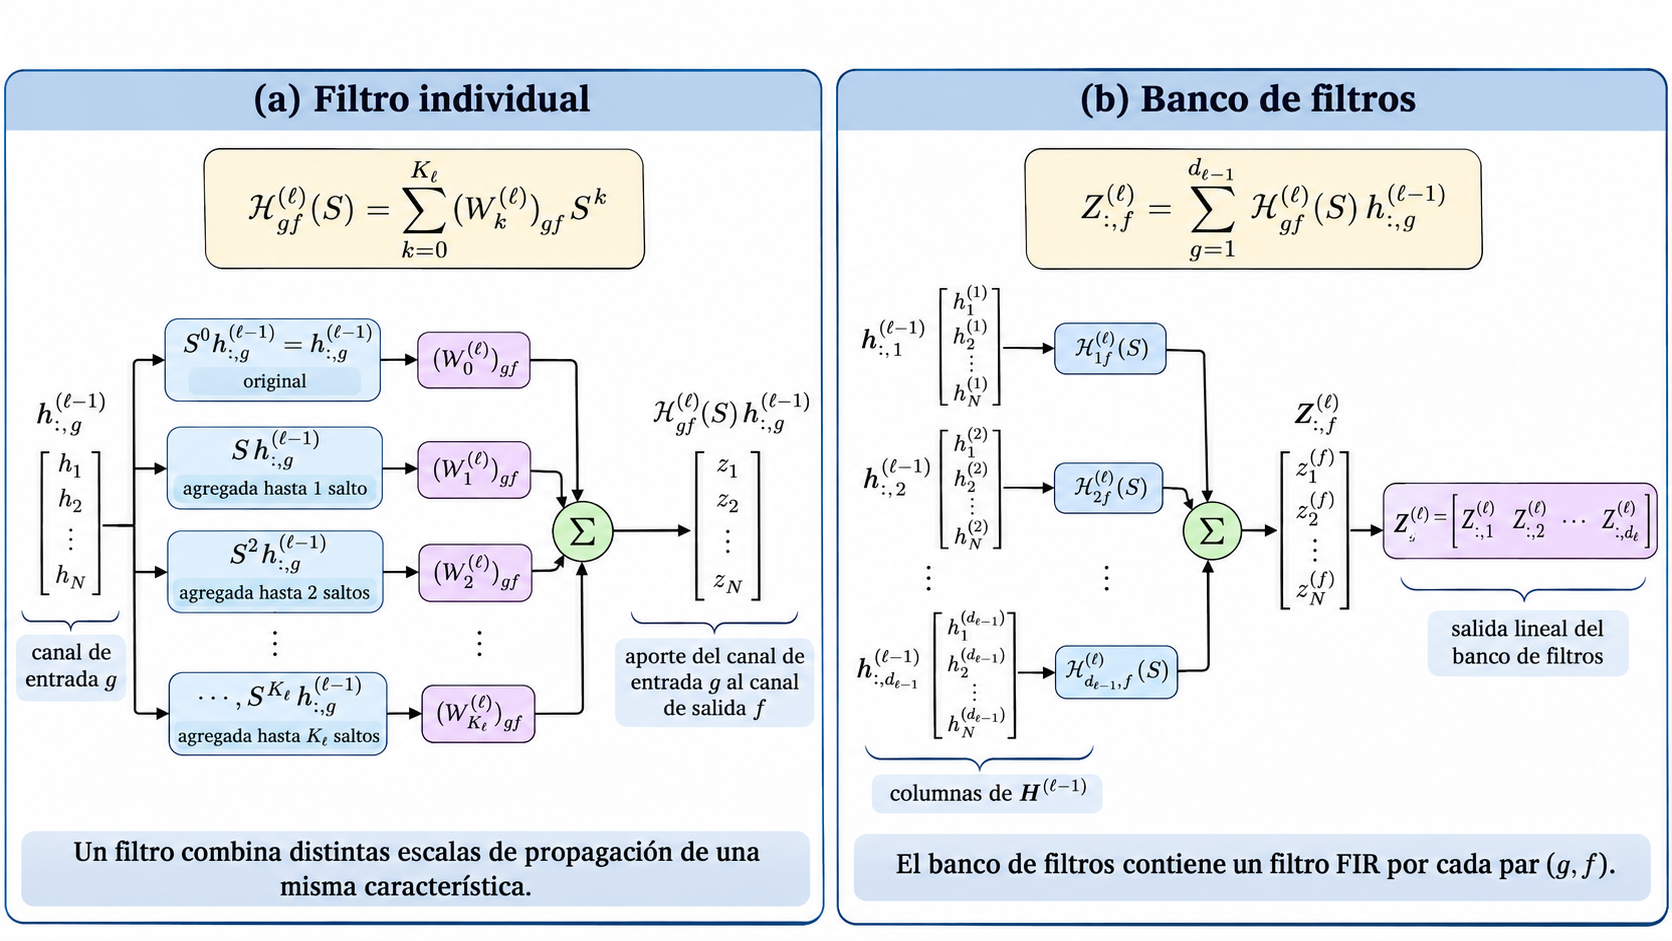
\includegraphics[width=1\linewidth]{infografía_de_filtros_fir_en_grafos.png}
    \caption{Filtro FIR individual y banco de filtros convolucionales multicanal sobre un grafo (en el diagrama, $N=n$ denota el número de vértices y $Z_*=Z^{(\ell)}$ la salida lineal de la capa).}
    \label{fig:filtros-fir-grafos}
\end{figure}

\begin{definicion}[Operador de actualización]
\label{def:gcnn-actualizacion}
Sea $\sigma_\ell:\mathbb R\to\mathbb R$ una función de activación, aplicada entrada a entrada a las matrices. Fijadas las matrices $W_0^{(\ell)},\ldots,W_{K_\ell}^{(\ell)}$, se define
\[
\begin{aligned}
\operatorname{UPDATE}_\ell:\bigl(\mathbb R^{n\times d_{\ell-1}}\bigr)^{K_\ell+1}
&\longrightarrow\mathbb R^{n\times d_\ell},\\
(M_0,\ldots,M_{K_\ell})
&\longmapsto\sigma_\ell\!\left(\sum_{k=0}^{K_\ell}M_kW_k^{(\ell)}\right).
\end{aligned}
\]
Al evaluar este operador en las matrices de agregación de la capa, se obtiene
\begin{equation}\label{eq:gcnn-actualizacion}
H^{(\ell)}:=\operatorname{UPDATE}_\ell\bigl(M_0^{(\ell)},\ldots,M_{K_\ell}^{(\ell)}\bigr)
=\sigma_\ell(Z^{(\ell)})
=\sigma_\ell\!\left(\sum_{k=0}^{K_\ell}M_k^{(\ell)}W_k^{(\ell)}\right).
\end{equation}
Para un vértice $v_i$, esta misma actualización se expresa mediante
\[
h_i^{(\ell)}=\sigma_\ell\!\left(\sum_{k=0}^{K_\ell}m_{k,i}^{(\ell)}W_k^{(\ell)}\right),
\qquad i=1,\ldots,n.
\]
Las expresiones matricial y por vértice describen la misma operación: la primera calcula todas las filas a la vez y la segunda corresponde únicamente al vértice $v_i$.
\end{definicion}

\begin{figure}[H]
    \centering
    \includegraphics[width=\textwidth]
    {\detokenize{infografía_del_operador_gcnn_en_español.png}}
    \caption{Operador de actualización en una capa GCNN:
    (a) actualización de las características de un vértice;
    (b) actualización matricial de toda la capa.}
    \label{fig:gcnn-update}
\end{figure}

\begin{definicion}[Aplicación de una capa convolucional sobre grafos]
\label{def:gcnn-capa}
Fijados el operador $S$, la función de activación $\sigma_\ell$ y los parámetros $W_0^{(\ell)},\ldots,W_{K_\ell}^{(\ell)}$, se define la aplicación asociada a la capa $\ell$ mediante
\begin{equation}\label{eq:gcnn-capa}
\begin{aligned}
\mathcal T_\ell:\mathbb R^{n\times d_{\ell-1}}&\longrightarrow\mathbb R^{n\times d_\ell},\\
H&\longmapsto\sigma_\ell\!\left(\sum_{k=0}^{K_\ell}S^kHW_k^{(\ell)}\right).
\end{aligned}
\end{equation}
En consecuencia, $H^{(\ell)}=\mathcal T_\ell(H^{(\ell-1)})$. En efecto, la aplicación $\mathcal T_\ell$ reúne la evaluación de las agregaciones multiescala y la posterior actualización de sus resultados.

\textbf{Verificación de las dimensiones.} Para $H\in\mathbb R^{n\times d_{\ell-1}}$, se tiene $S^kH\in\mathbb R^{n\times d_{\ell-1}}$ y $S^kHW_k^{(\ell)}\in\mathbb R^{n\times d_\ell}$. Por tanto, la suma finita de estos productos pertenece a $\mathbb R^{n\times d_\ell}$ y la activación conserva las dimensiones de la matriz.
\end{definicion}

\begin{definicion}[Capa de salida para clasificación binaria]
\label{def:gcnn-salida}
Para la clasificación binaria de los vértices del grafo se considera una GCNN cuya última capa satisface $d_{L_{\mathrm{net}}}=1$ y cuya activación es la función sigmoide,
\[
\sigma_{L_{\mathrm{net}}}(z)=\frac1{1+e^{-z}},\qquad z\in\mathbb R.
\]
En este caso, la última capa produce
\[
H^{(L_{\mathrm{net}})}=
\sigma_{L_{\mathrm{net}}}\!\left(
\sum_{k=0}^{K_{L_{\mathrm{net}}}}S^kH^{(L_{\mathrm{net}}-1)}W_k^{(L_{\mathrm{net}})}
\right)\in(0,1)^{n\times1}.
\]
Cada fila de $H^{(L_{\mathrm{net}})}$ contiene un único valor entre cero y uno correspondiente a un vértice.
\end{definicion}

\begin{definicion}[Red neuronal convolucional multicanal sobre grafos]
\label{def:gcnn-red}
Sean $\mathcal T_1,\ldots,\mathcal T_{L_{\mathrm{net}}}$ las aplicaciones de la Definición~\ref{def:gcnn-capa}. Se considera el conjunto de parámetros entrenables
\[
\theta=\bigl\{W_k^{(\ell)}:1\le\ell\le L_{\mathrm{net}},\ 0\le k\le K_\ell\bigr\}.
\]
La \emph{red neuronal convolucional multicanal sobre grafos} (GCNN) se define como la aplicación
\begin{equation}\label{eq:gcnn-red-completa}
\begin{aligned}
\Phi(\,\cdot\,;S,\theta):\mathbb R^{n\times d_0}&\longrightarrow\mathbb R^{n\times d_{L_{\mathrm{net}}}},\\
X&\longmapsto(\mathcal T_{L_{\mathrm{net}}}\circ\cdots\circ\mathcal T_1)(X).
\end{aligned}
\end{equation}
Por construcción, $\Phi(X;S,\theta)=H^{(L_{\mathrm{net}})}$.
\end{definicion}

\begin{figure}[H]
    \centering
    \includegraphics[width=\textwidth]
    {\detokenize{arquitectura_GCNN_composicion_sin_recuadros.png}}
    \caption{Arquitectura de una red neuronal convolucional
    multicanal sobre grafos, construida mediante la composición
    de capas convolucionales.}
    \label{fig:arquitectura-gcnn}
\end{figure}

\begin{definicion}[Probabilidad condicional de fraude y su estimación mediante una GCNN]
\label{def:probabilidad-fraude}

Sea $G=(V,E)$ un grafo que representa un conjunto de transacciones, con matriz de características $X$ y operador de desplazamiento $S$.

Para cada vértice $v_i\in V$, consideremos la variable aleatoria

\[
Y_i=
\begin{cases}
1, & \text{si la transacción asociada a }v_i\text{ es fraudulenta},\\
0, & \text{si la transacción asociada a }v_i\text{ es legítima}.
\end{cases}
\]

Considerando $X$ y $S$ como objetos aleatorios en la formulación poblacional, definimos la función

\[
\boxed{
\eta_i(x,s):=
\mathbb P(Y_i=1\mid X=x,S=s),
}
\]

que representa la probabilidad condicional verdadera de fraude, dadas las características $x$ y la estructura del grafo representada por $s$.

En consecuencia, $\mathbb P(Y_i=0\mid X=x,S=s)=1-\eta_i(x,s)$. Dado que la función $\eta_i$ es desconocida, consideramos una red neuronal convolucional sobre grafos $\Phi(\cdot;S,\theta)$, cuya salida correspondiente al vértice $v_i$ está dada por

\[
p_i(\theta;x,s):=
[\Phi(x;s,\theta)]_{i1}\in(0,1).
\]

El objetivo del modelo es determinar parámetros $\theta$ tales que

\[
\boxed{
p_i(\theta;x,s)\approx\eta_i(x,s).
}
\]

De este modo, interpretamos $p_i(\theta;x,s)$ como la probabilidad condicional de fraude estimada por la GCNN, mientras que $1-p_i(\theta;x,s)$ representa la probabilidad estimada de que la transacción sea legítima.

Finalmente, dado que durante el entrenamiento se consideran fijas las matrices observadas $x_{\mathrm{obs}}$ y $s_{\mathrm{obs}}$, \textbf{en adelante denotaremos simplemente por}

\[
\boxed{
p_i(\theta):=
p_i(\theta;x_{\mathrm{obs}},s_{\mathrm{obs}}).
}
\]

En consecuencia, identificando $X=x_{\mathrm{obs}}$ y $S=s_{\mathrm{obs}}$ en el conjunto de datos observado, la salida de la GCNN queda expresada por

\[
p(\theta):=\Phi(X;S,\theta)
=
\begin{pmatrix}
p_1(\theta)\\
\vdots\\
p_n(\theta)
\end{pmatrix}
\in(0,1)^{n\times 1}.
\]

\end{definicion}

\begin{proposicion}[Número de parámetros entrenables]
\label{prop:gcnn-parametros}
La red anterior contiene
\[
p=\sum_{\ell=1}^{L_{\mathrm{net}}}(K_\ell+1)d_{\ell-1}d_\ell
\]
parámetros escalares entrenables.
\end{proposicion}

\begin{proof}
Para cada capa $\ell$, existen $K_\ell+1$ matrices de parámetros $W_0^{(\ell)},\ldots,W_{K_\ell}^{(\ell)}$. Cada matriz pertenece a $\mathbb R^{d_{\ell-1}\times d_\ell}$ y contiene $d_{\ell-1}d_\ell$ entradas. Por tanto, la capa $\ell$ contiene $(K_\ell+1)d_{\ell-1}d_\ell$ parámetros escalares. Sumando sobre todas las capas se obtiene la expresión afirmada.
\end{proof}

\begin{ejemplo}[Capa multiescala de orden dos]
\label{ej:gcnn-multiescala-orden-dos}
Consideremos, para ilustrar el cálculo de una capa, el grafo de tres vértices con matriz de adyacencia
\[
A=\begin{pmatrix}
0&2&0\\2&0&1\\0&1&0
\end{pmatrix}.
\]
Se trata de un ejemplo independiente del grafo de nueve vértices utilizado en el capítulo anterior. Su operador normalizado, obtenido mediante la Definición~\ref{def:desplazamiento-normalizado}, y su matriz de características inicial son
\[
S=\begin{pmatrix}
\frac13&\frac1{\sqrt3}&0\\
\frac1{\sqrt3}&\frac14&\frac1{\sqrt8}\\
0&\frac1{\sqrt8}&\frac12
\end{pmatrix},
\qquad
H^{(0)}=\begin{pmatrix}1&0\\0&1\\1&1\end{pmatrix}.
\]
Tomemos $K_1=2$, $d_0=d_1=2$ y matrices de parámetros
\[
W_0^{(1)}=\begin{pmatrix}1&0\\0&1\end{pmatrix},\quad
W_1^{(1)}=\begin{pmatrix}1&0\\0&2\end{pmatrix},\quad
W_2^{(1)}=\begin{pmatrix}0&1\\1&0\end{pmatrix}.
\]
Se calculan las tres agregaciones $M_0^{(1)}=H^{(0)}$, $M_1^{(1)}=SH^{(0)}$ y $M_2^{(1)}=S^2H^{(0)}$. La salida lineal es $Z^{(1)}=M_0^{(1)}W_0^{(1)}+M_1^{(1)}W_1^{(1)}+M_2^{(1)}W_2^{(1)}$.

Calculando las dos matrices no triviales de agregación, obtenemos (con redondeo a cuatro decimales)
\[
M_1^{(1)}\approx\begin{pmatrix}
0.3333&0.5774\\0.9309&0.6036\\0.5000&0.8536
\end{pmatrix},\qquad
M_2^{(1)}\approx\begin{pmatrix}
0.6486&0.5409\\0.6020&0.7860\\0.5791&0.6402
\end{pmatrix}.
\]
Por tanto,
\[
Z^{(1)}\approx\begin{pmatrix}
1.8742&1.8033\\1.7169&2.8091\\2.1402&3.2862
\end{pmatrix}.
\]
Tomando $\sigma_1=\operatorname{ReLU}$, resulta $H^{(1)}=\operatorname{ReLU}(Z^{(1)})=Z^{(1)}$, pues todas las entradas de $Z^{(1)}$ son positivas.

El cálculo utiliza las escalas $k=0,1,2$ de la arquitectura general.
\end{ejemplo}

\chapter{Formulación del problema de optimización}

\section{Función de pérdida}\label{sec:funcion-perdida}

\subsection{Etiquetas observadas y datos de entrenamiento}

Sea $I_{\mathrm{tr}}\subseteq\{1,\ldots,n\}$ el conjunto de índices de los vértices etiquetados para entrenamiento, con

\[
m:=|I_{\mathrm{tr}}|>0.
\]

Para cada $i\in I_{\mathrm{tr}}$, sea $y_i\in\{0,1\}$ la realización observada de $Y_i$, asociada al vértice $v_i$ y, por tanto, a la fila $i$-ésima de $X$.

Considerando las matrices $X$ y $S$ fijadas, los datos de entrenamiento quedan representados por

\[
\boxed{
\mathcal D_{\mathrm{tr}}
=
\left(X,S,\{(i,y_i):i\in I_{\mathrm{tr}}\}\right).
}
\]

Dado que las probabilidades condicionales verdaderas $\eta_i$ son desconocidas, el ajuste de los parámetros $\theta$ se realizará a partir de las predicciones $p_i(\theta)$ y las etiquetas observadas $y_i$, para $i\in I_{\mathrm{tr}}$.

\subsection{Pérdida individual}

\begin{definicion}[Pérdida individual de entropía cruzada binaria]\label{def:perdida-individual}

Para cada $i\in I_{\mathrm{tr}}$, se define la función
$f_i:\mathbb{R}^p\to\mathbb{R}$ mediante

\[
\boxed{
f_i(\theta)
:=
-y_i\log p_i(\theta)
-(1-y_i)\log(1-p_i(\theta)).
}
\]

Esta función recibe el nombre de entropía cruzada binaria individual.

\end{definicion}

\begin{proposicion}[Caracterización de la pérdida individual]\label{prop:caracterizacion-perdida-individual}

Para cada $i\in I_{\mathrm{tr}}$ y todo $\theta\in\mathbb{R}^p$, se cumple

\[
f_i(\theta)
=
-\log\left(1-|p_i(\theta)-y_i|\right).
\]

En particular, $f_i(\theta)>0$. Además, para toda sucesión
$(\theta_r)_{r\in\mathbb{N}}\subseteq\mathbb{R}^p$,

\[
f_i(\theta_r)\longrightarrow 0
\quad\Longleftrightarrow\quad
p_i(\theta_r)\longrightarrow y_i.
\]

\end{proposicion}

\begin{proof}

Fijemos $i\in I_{\mathrm{tr}}$.

Si $y_i=1$, entonces $
f_i(\theta)=-\log p_i(\theta).
$ Como $0<p_i(\theta)<1$, se tiene $
1-|p_i(\theta)-1|=p_i(\theta),
$ y por tanto, $
f_i(\theta)
=
-\log\left(1-|p_i(\theta)-y_i|\right).
$ Si $y_i=0$, entonces $
f_i(\theta)=-\log(1-p_i(\theta)).
$ Dado que $|p_i(\theta)|=p_i(\theta)$, se obtiene la misma identidad. Además, $
0<1-|p_i(\theta)-y_i|<1,
$ de donde $f_i(\theta)>0$.

Para probar la equivalencia, la identidad anterior implica

\[
|p_i(\theta_r)-y_i|
=
1-e^{-f_i(\theta_r)}.
\]

Si $f_i(\theta_r)\to 0$, por continuidad de la función exponencial,

\[
|p_i(\theta_r)-y_i|\longrightarrow 0 \quad \text{por consiguiente} \quad p_i(\theta_r)\longrightarrow y_i.
\]

Recíprocamente, si $p_i(\theta_r)\to y_i$, entonces $
1-|p_i(\theta_r)-y_i|\longrightarrow 1.
$

Por continuidad del logaritmo en $1$,

\[
f_i(\theta_r)
=
-\log\left(1-|p_i(\theta_r)-y_i|\right)
\longrightarrow 0.\qedhere
\]
\end{proof}

% Procedencia: ejemplo construido (IA, Claude, 2026-11-23); números verificados
% con aritmética exacta en codigo/ejemplos_verificables.py (ejemplo A). review_pending.
\begin{ejemplo}[Valores de la pérdida individual]\label{ej:perdida-individual}
Supóngase que, para cierto $\theta$, la red asigna a un vértice $i\in I_{\mathrm{tr}}$ la probabilidad $p_i(\theta)=0{,}8$. Si $y_i=1$, la Proposición~\ref{prop:caracterizacion-perdida-individual} da
\[
f_i(\theta)=-\log(1-|0{,}8-1|)=-\log 0{,}8\approx 0{,}2231;
\]
si, en cambio, $y_i=0$, entonces
\[
f_i(\theta)=-\log(1-|0{,}8-0|)=-\log 0{,}2\approx 1{,}6094.
\]
La misma predicción se penaliza unas $7{,}2$ veces más cuando contradice la etiqueta observada. Además, si $y_i=0$ y $p_i(\theta_r)\to 1$, entonces $f_i(\theta_r)=-\log(1-p_i(\theta_r))\to\infty$: la pérdida no está acotada superiormente, aunque sí inferiormente por $0$.
\end{ejemplo}

\subsection{Función de pérdida empírica}

\begin{definicion}[Función de pérdida empírica]\label{def:perdida-empirica}

Se define la función de pérdida empírica
$F:\mathbb{R}^p\to\mathbb{R}$ mediante

\[
F(\theta):=\frac{1}{m}\sum_{i\in I_{\mathrm{tr}}}f_i(\theta).
\]

Por la Proposición~\ref{prop:caracterizacion-perdida-individual}, equivalentemente,

\[
\boxed{
F(\theta)
=-\frac{1}{m}\sum_{i\in I_{\mathrm{tr}}}
\log\left(1-|p_i(\theta)-y_i|\right).
}
\]

Esta función representa el promedio de las pérdidas individuales correspondientes a los vértices de entrenamiento.

\end{definicion}

\begin{proposicion}[Caracterización de la pérdida empírica]\label{prop:caracterizacion-perdida-empirica}

Para toda sucesión
$(\theta_r)_{r\in\mathbb{N}}\subseteq\mathbb{R}^p$,
se cumple

\[
\boxed{
\lim_{r\to\infty}F(\theta_r)=0
\quad\Longleftrightarrow\quad
\lim_{r\to\infty}p_i(\theta_r)=y_i,
\quad \forall i\in I_{\mathrm{tr}}.
}
\]

\end{proposicion}

\begin{proof}

Supongamos que

\[
\lim_{r\to\infty}F(\theta_r)=0.
\]

Por la Proposición~\ref{prop:caracterizacion-perdida-individual}, se tiene
$f_i(\theta_r)>0$ para todo $i\in I_{\mathrm{tr}}$.
En consecuencia, para cada $i\in I_{\mathrm{tr}}$,

\[
0\leq f_i(\theta_r)
\leq \sum_{j\in I_{\mathrm{tr}}}f_j(\theta_r)
=mF(\theta_r).
\]

Dado que $m>0$ es constante y
$F(\theta_r)\to 0$, por el teorema del sándwich,

\[
\lim_{r\to\infty}f_i(\theta_r)=0,
\qquad \forall i\in I_{\mathrm{tr}}.
\]

Aplicando nuevamente la Proposición~\ref{prop:caracterizacion-perdida-individual}, resulta

\[
\lim_{r\to\infty}p_i(\theta_r)=y_i,
\qquad \forall i\in I_{\mathrm{tr}}.
\]

Recíprocamente, supongamos que

\[
\lim_{r\to\infty}p_i(\theta_r)=y_i,
\qquad \forall i\in I_{\mathrm{tr}}.
\]

Por la Proposición~\ref{prop:caracterizacion-perdida-individual},

\[
\lim_{r\to\infty}f_i(\theta_r)=0,
\qquad \forall i\in I_{\mathrm{tr}}.
\]

Como $I_{\mathrm{tr}}$ es finito y $m>0$, se obtiene

\[
\begin{aligned}
\lim_{r\to\infty}F(\theta_r)
&=\lim_{r\to\infty}
\frac{1}{m}\sum_{i\in I_{\mathrm{tr}}}f_i(\theta_r)=\frac{1}{m}\sum_{i\in I_{\mathrm{tr}}}
\lim_{r\to\infty}f_i(\theta_r)=0.
\end{aligned}
\]

Esto concluye la demostración.
\end{proof}

% Procedencia: ejemplo construido (IA, Claude, 2026-11-23); números verificados
% con aritmética exacta en codigo/ejemplos_verificables.py (ejemplo B). review_pending.
\begin{ejemplo}[Un solo vértice mal ajustado impide que $F$ se anule]\label{ej:perdida-empirica}
Sean $I_{\mathrm{tr}}=\{1,2,3\}$, $m=3$, con etiquetas $(y_1,y_2,y_3)=(1,0,1)$, y supóngase que para cierto $\theta$ las predicciones son $(p_1,p_2,p_3)=(0{,}9;\,0{,}2;\,0{,}6)$. Entonces
\[
F(\theta)=-\tfrac13\bigl(\log 0{,}9+\log 0{,}8+\log 0{,}6\bigr)\approx 0{,}2798.
\]
Como cada $f_j$ es positiva, $F(\theta)\ge \frac13 f_i(\theta)$ para cada $i$; con $i=3$ resulta $F(\theta)\ge -\frac13\log 0{,}6\approx 0{,}1703$. En consecuencia, si una sucesión $(\theta_r)$ cumple $p_1(\theta_r)\to 1$ y $p_2(\theta_r)\to 0$, pero $p_3(\theta_r)=0{,}6$ para todo $r$, entonces $F(\theta_r)\ge 0{,}1703$ para todo $r$ y $F(\theta_r)\not\to 0$. Así, en la Proposición~\ref{prop:caracterizacion-perdida-empirica} la convergencia $p_i(\theta_r)\to y_i$ debe darse en \emph{todos} los vértices de entrenamiento.
\end{ejemplo}

\section{Problema de entrenamiento}\label{sec:problema-entrenamiento}

El entrenamiento de la GCNN se plantea como el siguiente problema de optimización no restringida:

\[
\boxed{
\min_{\theta\in\mathbb{R}^p}F(\theta),
}
\]
donde $F$ es la función de pérdida empírica definida en la Sección~\ref{sec:funcion-perdida}.

\section{Método de optimización L-BFGS}

% Integración de la parte de Daniel (convergencia y experimentos L-BFGS).
% Nota de coordinación: la subsección siguiente es una redacción breve de IA
% (Claude, 2026-11-23) a partir de Andrei (2020), §1.4.6, pp. 38--39,
% ecs. (1.97)--(1.99) y Algoritmo 1.6; review_pending. Puede sustituirse por la
% exposición de Francisco si se sube a Overleaf.
\subsection{El método L-BFGS}
\label{subsec:lbfgs-algoritmo}

Los métodos cuasi-Newton de memoria limitada están concebidos para problemas no
restringidos de gran escala cuya matriz hessiana no puede calcularse ni
almacenarse con un costo razonable~\cite[§1.4.6, p.~38]{andrei2020}. Este es el
caso del problema de la sección anterior: una aproximación densa de
$\nabla^2F(\theta)$ ocupa $p^2$ números, mientras que el método L-BFGS solo
guarda unos pocos pares de vectores de $\mathbb{R}^p$.

Denotemos por $\theta_k\in\mathbb{R}^p$ los iterados y $g_k:=\nabla F(\theta_k)$.
Cada paso del método BFGS tiene la forma~\cite[ecs.~(1.97)--(1.99), p.~38]{andrei2020}
\begin{equation}\label{eq:bfgs-paso}
\theta_{k+1}=\theta_k-\alpha_k H_k g_k,\qquad k=0,1,\ldots,
\end{equation}
donde $\alpha_k>0$ es el tamaño de paso y $H_k$ aproxima la inversa de la
hessiana, actualizada mediante
\begin{equation}\label{eq:bfgs-inversa}
H_{k+1}=V_k^\top H_k V_k+\rho_k s_k s_k^\top,
\qquad
\rho_k=\frac{1}{y_k^\top s_k},
\qquad
V_k=I-\rho_k y_k s_k^\top,
\end{equation}
con $s_k:=\theta_{k+1}-\theta_k$ e $y_k:=g_{k+1}-g_k$.

Como $H_k$ es en general densa, L-BFGS no la almacena: conserva únicamente los
$M$ pares $\{s_i,y_i\}$ más recientes y, tras calcular un nuevo iterado,
reemplaza el par más antiguo por el par $\{s_k,y_k\}$ recién obtenido. El
operador $H_k$ queda definido implícitamente como el resultado de aplicar la
actualización~\eqref{eq:bfgs-inversa}, en orden cronológico y con los pares
almacenados, a una matriz inicial $H_k^{(0)}$. Andrei indica que bastan entre
$3$ y $11$ pares en problemas de gran escala~\cite[p.~38]{andrei2020}. El
producto $H_k g_k$ se calcula sin formar $H_k$, mediante la recursión de dos
lazos del Algoritmo~\ref{alg:lbfgs-dos-lazos}~\cite[Algoritmo~1.6, p.~39]{andrei2020}.

\begin{algorithm}[H]
\caption{Recursión de dos lazos: cálculo de $r=H_k g_k$}
\label{alg:lbfgs-dos-lazos}
\begin{algorithmic}[1]
\Require $g_k$; los $\ell\le\min\{k,M\}$ pares aceptados más recientes $(s_{i_1},y_{i_1}),\ldots,(s_{i_\ell},y_{i_\ell})$ y $\rho_{i_j}=(y_{i_j}^\top s_{i_j})^{-1}$ (con $i_1=k-\ell,\ldots,i_\ell=k-1$ si ningún par fue descartado); escalado $\gamma_k>0$.
\State $q\gets g_k$
\For{$j=\ell,\ell-1,\ldots,1$}
  \State $a_j\gets\rho_{i_j}\, s_{i_j}^\top q$
  \State $q\gets q-a_j\, y_{i_j}$
\EndFor
\State $r\gets H_k^{(0)}q$, con $H_k^{(0)}=\gamma_k I$
\For{$j=1,2,\ldots,\ell$}
  \State $b\gets\rho_{i_j}\, y_{i_j}^\top r$
  \State $r\gets r+(a_j-b)\, s_{i_j}$
\EndFor
\State \Return $r$ \Comment{$r=H_k g_k$}
\end{algorithmic}
\end{algorithm}

Para la matriz inicial se adopta la elección usual
$H_k^{(0)}=\gamma_k I$ con
\begin{equation}\label{eq:lbfgs-escalado}
\gamma_k=\frac{s_{k-1}^\top y_{k-1}}{\|y_{k-1}\|_2^2},\qquad k\ge 1
\end{equation}
(o con el último par aceptado $(s_{i_\ell},y_{i_\ell})$ si la salvaguarda de curvatura descartó algún paso previo), factor que intenta estimar el tamaño de la hessiana a lo largo de la
dirección de búsqueda más reciente; con ello la dirección queda bien escalada
y el paso $\alpha_k=1$ se acepta en la mayoría de las
iteraciones~\cite[p.~39]{andrei2020}. En $k=0$ (o si la memoria está vacía) no hay pares almacenados y el
Algoritmo~\ref{alg:lbfgs-dos-lazos} devuelve $r=\gamma_0 g_0$; en la
implementación se toma $\gamma_0=1/\max\{1,\|g_0\|_2\}$. El método completo,
tal como se implementó en la Sección~\ref{subsec:lbfgs-experimentos-elliptic},
se resume en el Algoritmo~\ref{alg:lbfgs-wolfe}; las condiciones de Wolfe
fuertes se precisan en la Definición~\ref{def:lbfgs-wolfe}.

\begin{algorithm}[H]
\caption{L-BFGS con búsqueda lineal de Wolfe fuerte}
\label{alg:lbfgs-wolfe}
\begin{algorithmic}[1]
\Require $\theta_0\in\mathbb{R}^p$; memoria $M\in\mathbb{N}$; $0<c_1<c_2<1$;
tolerancias $\varepsilon_g,\varepsilon_\theta>0$; tope $k_{\max}$.
\State $k\gets 0$, $g_0\gets\nabla F(\theta_0)$
\While{$\|g_k\|_2>\varepsilon_g$ \textbf{y} $k<k_{\max}$}
  \State Calcular $r=H_k g_k$ con el Algoritmo~\ref{alg:lbfgs-dos-lazos} y tomar $d_k\gets -r$
  \State Elegir $\alpha_k>0$ que satisfaga las condiciones de Wolfe fuertes
  \State $\theta_{k+1}\gets\theta_k+\alpha_k d_k$, $g_{k+1}\gets\nabla F(\theta_{k+1})$
  \State $s_k\gets\theta_{k+1}-\theta_k$, $y_k\gets g_{k+1}-g_k$
  \If{$s_k^\top y_k>0$}
    \State Almacenar $(s_k,y_k,\rho_k)$, descartando el par más antiguo si ya hay $M$
  \EndIf
  \If{$\|s_k\|_2/\max\{1,\|\theta_{k+1}\|_2\}\le\varepsilon_\theta$ en dos iteraciones consecutivas}
    \State \Return $\theta_{k+1}$
  \EndIf
  \State $k\gets k+1$
\EndWhile
\State \Return $\theta_k$
\end{algorithmic}
\end{algorithm}

\begin{observacion}\label{obs:lbfgs-algoritmo}
\begin{enumerate}
\item Si $d_k$ es dirección de descenso, la condición de curvatura de Wolfe
$g_{k+1}^\top d_k\ge c_2\,g_k^\top d_k$ implica
\[
s_k^\top y_k=\alpha_k\,(g_{k+1}-g_k)^\top d_k
\ge \alpha_k\,(c_2-1)\,g_k^\top d_k>0,
\]
pues $c_2<1$ y $g_k^\top d_k<0$. Por tanto $\rho_k>0$ está bien definido y la
prueba $s_k^\top y_k>0$ del Algoritmo~\ref{alg:lbfgs-wolfe} solo actúa como
salvaguarda numérica. Que $H_k$ sea definida positiva y que $d_k$ sea, en
efecto, de descenso se demuestra en la
Proposición~\ref{prop:convergencia-lbfgs}.
\item Cada llamada al Algoritmo~\ref{alg:lbfgs-dos-lazos} requiere $\ell$
productos escalares y $\ell$ actualizaciones vectoriales en cada lazo, es
decir, $4\ell p+p+2\ell$ multiplicaciones escalares ($4\ell p+p+\mathcal{O}(\ell)$), y la memoria almacena $2Mp$ números;
ambos costos son lineales en $p$.
\item En la implementación se añade una salvaguarda: si la dirección calculada
no es numéricamente de descenso o la búsqueda lineal no reduce $F$, se vacía la
memoria y se reinicia con $d_k=-g_k$. Bajo las hipótesis de la
Proposición~\ref{prop:convergencia-lbfgs} la dirección $d_k$ es siempre de
descenso, de modo que el reinicio solo responde a errores de redondeo, a
fallos de la búsqueda lineal práctica o a la falta de diferenciabilidad
(por ejemplo, con $\operatorname{ReLU}$).
\end{enumerate}
\end{observacion}

% Procedencia: ejemplo construido (IA, Claude, 2026-11-23); números verificados
% con aritmética exacta en codigo/ejemplos_verificables.py (ejemplo H). review_pending.
\begin{ejemplo}[Recursión de dos lazos con memoria $M=1$]\label{ej:dos-lazos}
Sea $p=2$ y supóngase almacenado un único par $s=(1,0)^\top$, $y=(2,1)^\top$, de modo que $s^\top y=2$, $\rho=\frac12$ y, por~\eqref{eq:lbfgs-escalado}, $\gamma=s^\top y/\|y\|_2^2=\frac25$. Para $g=(1,1)^\top$, el Algoritmo~\ref{alg:lbfgs-dos-lazos} con $\ell=1$ realiza:
\[
a=\rho\,s^\top g=\tfrac12,\quad q=g-a\,y=\bigl(0,\tfrac12\bigr)^\top,\quad r=\gamma q=\bigl(0,\tfrac15\bigr)^\top,\quad b=\rho\,y^\top r=\tfrac1{10},\quad r\gets r+(a-b)s=\bigl(\tfrac25,\tfrac15\bigr)^\top.
\]
Por otra parte, la actualización explícita~\eqref{eq:bfgs-inversa} aplicada a $\gamma I$, con $V=I-\rho\,y s^\top=\begin{pmatrix}0&0\\-\frac12&1\end{pmatrix}$, da
\[
H=V^\top(\gamma I)V+\rho\,ss^\top=\begin{pmatrix}\frac35&-\frac15\\[2pt]-\frac15&\frac25\end{pmatrix},
\qquad Hg=\bigl(\tfrac25,\tfrac15\bigr)^\top=r.
\]
La recursión obtiene $Hg$ sin formar la matriz $H$.
\end{ejemplo}

\subsection{Análisis de convergencia global del método L-BFGS}
\label{subsec:lbfgs-convergencia}

Para analizar la convergencia de un método de búsqueda lineal aplicado al
problema de optimización no restringida $\min_{\theta\in\mathbb{R}^p} F(\theta)$
planteado en la sección anterior, seguimos el marco de~\cite{andrei2020}
(Capítulo~3, Sección~3.3, pp.~89 y~97--100). Para evitar colisiones de notación
con los capítulos previos del presente informe, los iterados de parámetros se
denotan por $\theta_k\in\mathbb{R}^p$ (en lugar de $x_k\in\mathbb{R}^n$), el
gradiente en $\theta_k$ por $g_k:=\nabla F(\theta_k)$, el tamaño de memoria de
L-BFGS por $M\in\mathbb{N}$ (distinto de $m=|I_{\mathrm{tr}}|$), el ángulo entre
$-g_k$ y la dirección de búsqueda $d_k$ por $\psi_k$ (en lugar de $\theta_k$), y
los parámetros de Wolfe por $0<c_1<c_2<1$ (en lugar de $\rho$ y $\sigma$,
reservados respectivamente para $\rho_k=(y_k^\top s_k)^{-1}$ y para las
funciones de activación $\sigma_\ell$).

\begin{definicion}[Dirección de descenso, ángulo de búsqueda y condiciones de Wolfe]
\label{def:lbfgs-wolfe}
Sea $F:\mathbb{R}^p\to\mathbb{R}$ continuamente diferenciable y considérese una
sucesión generada por búsqueda lineal
\begin{equation}\label{eq:iteracion-busqueda-lineal}
\theta_{k+1}=\theta_k+\alpha_k d_k,\qquad k=0,1,2,\ldots,
\end{equation}
con tamaño de paso $\alpha_k>0$ y dirección $d_k\in\mathbb{R}^p$.
\begin{enumerate}
\item Se dice que $d_k$ es una \emph{dirección de descenso} en $\theta_k$ si
\begin{equation}\label{eq:condicion-descenso}
g_k^\top d_k < 0.
\end{equation}
\item Cuando $g_k\neq 0$ y $d_k\neq 0$, el ángulo $\psi_k\in[0,\pi]$ entre la
dirección de máximo descenso $-g_k$ y la dirección de búsqueda $d_k$ queda
caracterizado por
\begin{equation}\label{eq:coseno-angulo}
\cos\psi_k := -\frac{g_k^\top d_k}{\|g_k\|_2\,\|d_k\|_2}.
\end{equation}
Si $d_k$ es dirección de descenso, entonces $\cos\psi_k\in(0,1]$.
\item Fijadas constantes $0<c_1<c_2<1$, se dice que el paso $\alpha_k>0$
satisface las \emph{condiciones estándar de Wolfe}~\cite[ecs.~(3.4)--(3.5), p.~89]{andrei2020} si
\begin{align}
F(\theta_k+\alpha_k d_k) &\le F(\theta_k)+c_1\alpha_k g_k^\top d_k,
\label{eq:wolfe-armijo}\\
\nabla F(\theta_k+\alpha_k d_k)^\top d_k &\ge c_2 g_k^\top d_k.
\label{eq:wolfe-curvatura}
\end{align}
Si además se cumple
$|\nabla F(\theta_k+\alpha_k d_k)^\top d_k|\le -c_2 g_k^\top d_k$, se dice que
$\alpha_k$ satisface las \emph{condiciones fuertes de Wolfe}~\cite[ec.~(3.6), p.~89]{andrei2020};
en particular, toda búsqueda lineal de Wolfe fuerte satisface~\eqref{eq:wolfe-armijo}--\eqref{eq:wolfe-curvatura}.
\end{enumerate}
\end{definicion}

% Procedencia: ejemplo construido (IA, Claude, 2026-11-23); números verificados
% con aritmética exacta en codigo/ejemplos_verificables.py (ejemplo D). review_pending.
\begin{ejemplo}[Pasos que cumplen y que violan las condiciones de Wolfe]\label{ej:wolfe}
Sea $F(\theta)=\frac12\theta^\top A\theta$ con $A=\operatorname{diag}(1,4)$, $\theta_0=(1,1)^\top$ y $d_0=-g_0=(-1,-4)^\top$, de modo que $F(\theta_0)=\frac52$ y $g_0^\top d_0=-17$; tómense $c_1=10^{-4}$ y $c_2=0{,}9$. La función $\varphi(\alpha):=F(\theta_0+\alpha d_0)$ vale
\[
\varphi(\alpha)=\tfrac52-17\alpha+\tfrac{65}{2}\alpha^2,\qquad \varphi'(\alpha)=\nabla F(\theta_0+\alpha d_0)^\top d_0=-17+65\alpha.
\]
\begin{enumerate}
\item $\alpha=1$: $\varphi(1)=18>\frac52-17c_1$; se viola~\eqref{eq:wolfe-armijo}. El paso es demasiado largo.
\item $\alpha=\frac1{100}$: $\varphi(\frac1{100})=\frac{9333}{4000}\approx 2{,}3333$ cumple~\eqref{eq:wolfe-armijo}, pero $\varphi'(\frac1{100})=-16{,}35<c_2\,g_0^\top d_0=-15{,}3$; se viola~\eqref{eq:wolfe-curvatura}. El paso es demasiado corto.
\item $\alpha=\frac14$: $\theta_0+\frac14 d_0=(\frac34,0)^\top$, $\varphi(\frac14)=\frac{9}{32}$ y $|\varphi'(\frac14)|=\frac34\le 15{,}3$; se cumplen las condiciones fuertes de Wolfe.
\end{enumerate}
En general, la condición fuerte de curvatura $|\varphi'(\alpha)|\le 15{,}3$ equivale a $\alpha\in[\frac{17}{650},\frac{323}{650}]\approx[0{,}0262;\,0{,}4969]$, y en ese intervalo también se cumple~\eqref{eq:wolfe-armijo}, que vale para $\alpha\le\frac{34(1-c_1)}{65}\approx 0{,}5230$. El paso exacto $\alpha^*=\frac{17}{65}$, raíz de $\varphi'$, pertenece al intervalo; la búsqueda de Wolfe no necesita calcularlo.
\end{ejemplo}

El resultado fundamental para el análisis de convergencia global de los métodos
de búsqueda lineal con condiciones de Wolfe es el criterio de Zoutendijk.

% Corrección editorial (IA, 2026-11-23): en Andrei (2020), p. 98, ec. (3.33),
% aparece una errata tipográfica de signo: escribe f_{k+1} <= f_k + c cos^2(theta_k)||g_k||^2
% con c = rho(1-sigma)/L > 0, cuando de (3.32) sigue el signo menos (-c).
% Además se unifica el índice inicial a k >= 0 (coherente con el conjunto de nivel S en theta_0)
% y se explicita la pertenencia de los iterados a S \subset N.
\begin{teorema}[Condición de Zoutendijk~\cite{andrei2020}, Teorema~3.1, p.~98]
\label{thm:zoutendijk}
Supóngase que $F:\mathbb{R}^p\to\mathbb{R}$ satisface las hipótesis siguientes:
\begin{enumerate}
\item $F$ está acotada inferiormente en $\mathbb{R}^p$, es decir, existe
$F_{\inf}\in\mathbb{R}$ tal que $F(\theta)\ge F_{\inf}$ para todo
$\theta\in\mathbb{R}^p$.
\item $F$ es continuamente diferenciable en una vecindad abierta $\mathcal{N}$
del conjunto de nivel
\[
\mathcal{S}:=\{\theta\in\mathbb{R}^p : F(\theta)\le F(\theta_0)\}.
\]
\item El gradiente $\nabla F$ es Lipschitz continuo en $\mathcal{N}$, esto es,
existe una constante $L>0$ tal que
\begin{equation}\label{eq:gradiente-lipschitz}
\|\nabla F(\theta)-\nabla F(\tilde\theta)\|_2
\le L\|\theta-\tilde\theta\|_2,
\qquad \forall\,\theta,\tilde\theta\in\mathcal{N}.
\end{equation}
\end{enumerate}
Considérese una iteración de la forma~\eqref{eq:iteracion-busqueda-lineal} tal
que, para todo $k\ge 0$, se tiene $g_k\neq 0$, $d_k$ es una dirección de
descenso~\eqref{eq:condicion-descenso} y $\alpha_k>0$ satisface las condiciones
estándar de Wolfe~\eqref{eq:wolfe-armijo}--\eqref{eq:wolfe-curvatura} con
$0<c_1<c_2<1$. Entonces se cumple la \emph{condición de Zoutendijk}:
\begin{equation}\label{eq:zoutendijk}
\sum_{k=0}^{\infty}\cos^2\psi_k\,\|g_k\|_2^2 < \infty,
\end{equation}
o, equivalentemente,
\begin{equation}\label{eq:zoutendijk-equiv}
\sum_{k=0}^{\infty}\frac{(g_k^\top d_k)^2}{\|d_k\|_2^2} < \infty.
\end{equation}
\end{teorema}

\begin{proof}
En primer lugar verificamos por inducción que $\theta_k\in\mathcal{S}\subset\mathcal{N}$
para todo $k\ge 0$. Para $k=0$ la pertenencia $\theta_0\in\mathcal{S}$ es
inmediata. Si $\theta_k\in\mathcal{S}$, como $c_1>0$, $\alpha_k>0$ y
$g_k^\top d_k<0$, la condición~\eqref{eq:wolfe-armijo} implica
\[
F(\theta_{k+1}) \le F(\theta_k)+c_1\alpha_k g_k^\top d_k < F(\theta_k) \le F(\theta_0),
\]
de modo que $\theta_{k+1}\in\mathcal{S}\subset\mathcal{N}$.

Restando $g_k^\top d_k$ en ambos miembros de la condición de
curvatura~\eqref{eq:wolfe-curvatura}, se obtiene
\begin{equation}\label{eq:zout-paso1}
(g_{k+1}-g_k)^\top d_k \ge (c_2-1)g_k^\top d_k.
\end{equation}
Por otra parte, aplicando la desigualdad de Cauchy--Schwarz y la condición de
Lipschitz~\eqref{eq:gradiente-lipschitz} al par $\theta_k,\theta_{k+1}\in\mathcal{N}$,
resulta
\begin{equation}\label{eq:zout-paso2}
(g_{k+1}-g_k)^\top d_k
\le \|g_{k+1}-g_k\|_2\,\|d_k\|_2
\le L\|\theta_{k+1}-\theta_k\|_2\,\|d_k\|_2
= \alpha_k L\|d_k\|_2^2.
\end{equation}
Como $g_k^\top d_k<0$, necesariamente $d_k\neq 0$ y $L\|d_k\|_2^2>0$.
Combinando~\eqref{eq:zout-paso1} y~\eqref{eq:zout-paso2}, se deduce la cota
inferior sobre el tamaño de paso~\cite[ec.~(3.31), p.~98]{andrei2020}:
\begin{equation}\label{eq:cota-paso-wolfe}
\alpha_k \ge \frac{c_2-1}{L}\,\frac{g_k^\top d_k}{\|d_k\|_2^2}
= \frac{1-c_2}{L}\,\frac{(-g_k^\top d_k)}{\|d_k\|_2^2} > 0.
\end{equation}
Al multiplicar~\eqref{eq:cota-paso-wolfe} por $c_1 g_k^\top d_k<0$ se invierte
el sentido de la desigualdad y, sustituyendo en la condición de
Armijo~\eqref{eq:wolfe-armijo}, se obtiene
\[
F(\theta_{k+1})
\le F(\theta_k) + c_1\alpha_k g_k^\top d_k
\le F(\theta_k) + c_1\frac{c_2-1}{L}\,\frac{(g_k^\top d_k)^2}{\|d_k\|_2^2}.
\]
Usando la definición~\eqref{eq:coseno-angulo} de $\cos\psi_k$ y definiendo la
constante positiva $c:=c_1(1-c_2)/L>0$ (ya que $0<c_1<c_2<1$), la desigualdad
anterior se reescribe como
\begin{equation}\label{eq:descenso-zoutendijk}
F(\theta_{k+1}) \le F(\theta_k) - c\cos^2\psi_k\,\|g_k\|_2^2,
\qquad \forall\,k\ge 0.
\end{equation}
Reordenando~\eqref{eq:descenso-zoutendijk} y sumando desde $k=0$ hasta cualquier
$N\in\mathbb{N}$, la suma telescópica junto con la cota inferior $F(\theta_{N+1})\ge F_{\inf}$
produce
\[
c\sum_{k=0}^{N}\cos^2\psi_k\,\|g_k\|_2^2
\le \sum_{k=0}^{N}\bigl(F(\theta_k)-F(\theta_{k+1})\bigr)
= F(\theta_0)-F(\theta_{N+1})
\le F(\theta_0)-F_{\inf}.
\]
Dividiendo entre $c>0$, las sumas parciales de la serie de términos no negativos
quedan uniformemente acotadas por $(F(\theta_0)-F_{\inf})/c$, lo que establece
la convergencia~\eqref{eq:zoutendijk} y, por~\eqref{eq:coseno-angulo}, su forma
equivalente~\eqref{eq:zoutendijk-equiv}.
\end{proof}

Bajo una hipótesis adicional que impida que las direcciones de búsqueda tiendan
a hacerse ortogonales al gradiente, la condición de Zoutendijk implica el límite
de convergencia global a puntos estacionarios~\cite[ecs.~(3.35)--(3.36), p.~99]{andrei2020}.

\begin{corolario}[Convergencia global a puntos estacionarios~\cite{andrei2020}, ecs.~(3.35)--(3.36), p.~99]
\label{cor:convergencia-global-limite}
Bajo las hipótesis del Teorema~\ref{thm:zoutendijk}, supóngase además que existe
una constante $\delta>0$ tal que
\begin{equation}\label{eq:acotacion-coseno}
\cos\psi_k \ge \delta > 0, \qquad \forall\,k\ge 0.
\end{equation}
Entonces
\begin{equation}\label{eq:limite-gradiente-cero}
\lim_{k\to\infty}\|g_k\|_2 = 0.
\end{equation}
\end{corolario}

\begin{proof}
Por~\eqref{eq:acotacion-coseno}, para todo $k\ge 0$ se tiene
\[
0 \le \delta^2\|g_k\|_2^2 \le \cos^2\psi_k\,\|g_k\|_2^2.
\]
Como la serie~\eqref{eq:zoutendijk} converge, su término general tiende a cero:
$\lim_{k\to\infty}\cos^2\psi_k\|g_k\|_2^2=0$. Dado que $\delta^2>0$, se deduce
$\lim_{k\to\infty}\|g_k\|_2^2=0$ y, por continuidad de la raíz cuadrada,
$\lim_{k\to\infty}\|g_k\|_2=0$.
\end{proof}

A continuación mostramos cómo se verifican las condiciones de descenso y de
acotación angular~\eqref{eq:acotacion-coseno} en los métodos cuasi-Newton y en
particular en L-BFGS~\cite[Sección~1.4.6, pp.~38--39 y Sección~3.3, ítem~2, pp.~99--100]{andrei2020}.

\begin{proposicion}[Preservación de positividad y convergencia global de L-BFGS]
\label{prop:convergencia-lbfgs}
Considérese una iteración de tipo cuasi-Newton $d_k=-H_k g_k$ (con $H_k=B_k^{-1}$
simétrica en $\mathbb{R}^{p\times p}$) y paso $\alpha_k>0$ elegido según las
condiciones estándar de Wolfe~\eqref{eq:wolfe-armijo}--\eqref{eq:wolfe-curvatura}.
\begin{enumerate}
\item \textbf{Preservación de definición positiva en L-BFGS:} sean
$s_k:=\theta_{k+1}-\theta_k$ e $y_k:=g_{k+1}-g_k$. Si $d_k$ es de descenso,
entonces la condición de curvatura~\eqref{eq:wolfe-curvatura} garantiza
$s_k^\top y_k>0$. Además, si una matriz simétrica $H$ es definida positiva y
$s_k^\top y_k>0$, entonces la actualización inversa BFGS
$H^+ = V_k^\top H V_k + \rho_k s_k s_k^\top$ (con $\rho_k=(s_k^\top y_k)^{-1}$ y
$V_k = I - \rho_k y_k s_k^\top$) es también simétrica definida positiva. En
consecuencia, partiendo de $H_k^{(0)}=\gamma_k I\succ 0$ con
$\gamma_k=(s_{k-1}^\top y_{k-1})/\|y_{k-1}\|_2^2>0$ para $k\ge 1$ (o el último par aceptado si alguno fue omitido) y un
$\gamma_0>0$ fijado (en la implementación, $\gamma_0=1/\max\{1,\|g_0\|_2\}$), el operador implícito $H_k$
del algoritmo L-BFGS con memoria $M$ es simétrico definido positivo y genera una
dirección de descenso $d_k=-H_k g_k$ en cada iteración mientras $g_k\neq 0$.
\item \textbf{Criterio de convergencia global~\cite[pp.~99--100]{andrei2020}:}
si $F$ satisface las hipótesis del Teorema~\ref{thm:zoutendijk}, $H_k=B_k^{-1}\succ 0$
para todo $k\ge 0$ y el número de condición espectral está uniformemente acotado,
esto es, existe una constante $\Delta\ge 1$ tal que
\begin{equation}\label{eq:condicion-uniforme-lbfgs}
\kappa_2(B_k) := \|B_k\|_2\,\|B_k^{-1}\|_2 = \|H_k^{-1}\|_2\,\|H_k\|_2 \le \Delta,
\qquad \forall\,k\ge 0,
\end{equation}
entonces
\begin{equation}\label{eq:cota-coseno-cuasinewton}
\cos\psi_k \ge \frac{1}{\Delta} > 0, \qquad \forall\,k\ge 0,
\end{equation}
y, por el Corolario~\ref{cor:convergencia-global-limite}, se verifica
$\lim_{k\to\infty}\|g_k\|_2 = 0$.
\end{enumerate}
\end{proposicion}

\begin{proof}
\emph{Parte~1.} Por~\eqref{eq:wolfe-curvatura}, $\alpha_k>0$, $c_2<1$ y
$g_k^\top d_k<0$, resulta
\[
s_k^\top y_k = \alpha_k (g_{k+1}-g_k)^\top d_k
\ge \alpha_k (c_2-1) g_k^\top d_k
= \alpha_k (1-c_2)(-g_k^\top d_k) > 0.
\]
En particular $\rho_k=(s_k^\top y_k)^{-1}>0$. La simetría de $H^+$ es inmediata
a partir de la simetría de $H$. Para todo $v\in\mathbb{R}^p\setminus\{0\}$,
\[
v^\top H^+ v = (V_k v)^\top H (V_k v) + \rho_k (s_k^\top v)^2 \ge 0.
\]
Si se tuviera $v^\top H^+ v=0$, la definición positiva de $H$ y $\rho_k>0$
forzarían $s_k^\top v=0$ y $V_k v=0$; pero cuando $s_k^\top v=0$ se cumple
$V_k v = v - \rho_k(s_k^\top v)y_k = v$, contradiciendo $v\neq 0$. Luego
$H^+\succ 0$. Aplicando inductivamente esta propiedad a las actualizaciones con
los últimos $\min\{k,M\}$ pares almacenados a partir de $H_k^{(0)}=\gamma_k I\succ 0$,
se concluye que $H_k\succ 0$ y, por tanto, $g_k^\top d_k=-g_k^\top H_k g_k<0$ para
todo $g_k\neq 0$.

\emph{Parte~2.} Como $H_k=B_k^{-1}$ es simétrica definida positiva, sus valores
propios son reales y estrictamente positivos, de modo que en la norma espectral
inducida por la norma euclidiana se tiene $\|H_k\|_2=\lambda_{\max}(H_k)$ y
$\|H_k^{-1}\|_2=\|B_k\|_2=1/\lambda_{\min}(H_k)$. Por el cociente de Rayleigh,
para todo $g_k\neq 0$:
\[
-g_k^\top d_k = g_k^\top H_k g_k \ge \lambda_{\min}(H_k)\|g_k\|_2^2
= \frac{\|g_k\|_2^2}{\|B_k\|_2} > 0,
\]
mientras que la submultiplicatividad de la norma espectral implica
\[
\|d_k\|_2 = \|H_k g_k\|_2 \le \|H_k\|_2\|g_k\|_2 = \|B_k^{-1}\|_2\|g_k\|_2.
\]
Sustituyendo ambas acotaciones en~\eqref{eq:coseno-angulo} y usando~\eqref{eq:condicion-uniforme-lbfgs}:
\[
\cos\psi_k
= \frac{g_k^\top H_k g_k}{\|g_k\|_2\,\|H_k g_k\|_2}
\ge \frac{\|g_k\|_2^2 / \|B_k\|_2}{\|g_k\|_2\,\|B_k^{-1}\|_2\,\|g_k\|_2}
= \frac{1}{\|B_k\|_2\,\|B_k^{-1}\|_2}
\ge \frac{1}{\Delta} > 0.
\]
Aplicando el Corolario~\ref{cor:convergencia-global-limite} con $\delta:=1/\Delta$,
se obtiene finalmente $\lim_{k\to\infty}\|g_k\|_2=0$.
\end{proof}

% Procedencia: ejemplo construido (IA, Claude, 2026-11-23); números verificados
% con aritmética exacta en codigo/ejemplos_verificables.py (ejemplo E). review_pending.
\begin{ejemplo}[La cota angular es válida pero no ajustada]\label{ej:cota-coseno}
Sean $H=\operatorname{diag}(1,\frac14)$, de modo que $B=H^{-1}=\operatorname{diag}(1,4)$ y $\kappa_2(B)=4$, y $g=(1,1)^\top$. Entonces $d=-Hg=(-1,-\frac14)^\top$, $-g^\top d=\frac54$, $\|g\|_2=\sqrt2$, $\|d\|_2=\frac{\sqrt{17}}4$ y
\[
\cos\psi=\frac{5/4}{\sqrt2\,\sqrt{17}/4}=\frac{5}{\sqrt{34}}\approx 0{,}857\ \ge\ \frac1{\kappa_2(B)}=\frac14 .
\]
La cota~\eqref{eq:cota-coseno-cuasinewton} con $\Delta=4$ se cumple con amplio margen: es una garantía del peor caso, no una estimación del ángulo efectivo.
\end{ejemplo}

% Procedencia: ejemplo construido (IA, Claude, 2026-11-23); números verificados
% con aritmética exacta en codigo/ejemplos_verificables.py (ejemplo F). review_pending.
\begin{ejemplo}[La actualización BFGS preserva la definición positiva]\label{ej:bfgs-positiva}
Con el par $s=(1,0)^\top$, $y=(2,1)^\top$ del Ejemplo~\ref{ej:dos-lazos} ($s^\top y=2>0$) y $H=I$, la actualización de la Proposición~\ref{prop:convergencia-lbfgs} da
\[
H^+=V^\top V+\tfrac12 ss^\top=\begin{pmatrix}\frac34&-\frac12\\[2pt]-\frac12&1\end{pmatrix}.
\]
Se verifica la ecuación secante $H^+y=s$, y $H^+\succ 0$, pues $H^+_{11}=\frac34>0$ y $\det H^+=\frac12>0$.
\end{ejemplo}

% Procedencia: ejemplo construido (IA, Claude, 2026-11-23); números verificados
% con aritmética exacta en codigo/ejemplos_verificables.py (ejemplo G). review_pending.
\begin{ejemplo}[Contraejemplo: sin curvatura positiva se pierde la definición positiva]\label{ej:contraejemplo-curvatura}
Sean $s=(1,0)^\top$, $y=(-1,1)^\top$, con $s^\top y=-1<0$, y $H=I$. La misma fórmula, con $\rho=-1$ y $V=I-\rho\,ys^\top=\begin{pmatrix}0&0\\1&1\end{pmatrix}$, produce
\[
H^+=V^\top V-ss^\top=\begin{pmatrix}0&1\\1&1\end{pmatrix},\qquad \det H^+=-1,
\]
y para $v=(1,-1)^\top$ se tiene $v^\top H^+v=-1<0$: $H^+$ es indefinida y $-H^+g$ puede no ser dirección de descenso. Un par así surge en una función no convexa: para $F(\theta)=-\frac12\theta^2$ en $\mathbb{R}$, con $\theta_0=1$, $d_0=1$ (dirección de descenso, $g_0d_0=-1$) y $\alpha=1$, resulta $s_0=1$, $y_0=g_1-g_0=-1$ y $s_0y_0=-1$. La condición~\eqref{eq:wolfe-curvatura} rechaza ese paso, pues $g_1d_0=-2<c_2\,g_0d_0=-0{,}9$; de hecho, $\nabla F(\theta_0+\alpha d_0)\,d_0=-(1+\alpha)<-0{,}9$ para todo $\alpha>0$, de modo que ningún paso cumple~\eqref{eq:wolfe-curvatura}, lo que es compatible con que esta $F$ no está acotada inferiormente. Este es el papel de la salvaguarda de la Observación~\ref{obs:lbfgs-algoritmo}: descartar pares con $s_k^\top y_k\le 0$.
\end{ejemplo}

\begin{observacion}[Alcance de las hipótesis teóricas en el entrenamiento de la GCNN]
\label{obs:hipotesis-gcnn-lbfgs}
El Teorema~\ref{thm:zoutendijk} y el Corolario~\ref{cor:convergencia-global-limite}
\emph{no} exigen convexidad de la función objetivo, lo que los hace pertinentes
para el entrenamiento de redes neuronales. Sin embargo, al contrastarlos con la
función de pérdida empírica $F(\theta)$ de la GCNN conviene precisar cuatro
aspectos:
\begin{enumerate}
\item \textbf{Acotación inferior:} por la caracterización de la pérdida
individual, $f_i(\theta)>0$ para todo $i\in I_{\mathrm{tr}}$ y todo
$\theta\in\mathbb{R}^p$, luego $F(\theta)>0$ y la hipótesis~1 del
Teorema~\ref{thm:zoutendijk} se satisface con $F_{\inf}=0$.
\item \textbf{Diferenciabilidad y regularidad Lipschitz del gradiente:} si las
activaciones ocultas $\sigma_\ell$ son de clase $C^2$, la composición de las
aplicaciones polinomiales en $\theta$, $\sigma_\ell$, la sigmoide final y la
entropía cruzada binaria produce $F\in C^2(\mathbb{R}^p)$; si $\sigma_\ell$ es de
clase $C^\infty$ (por ejemplo $\tanh$ o $\operatorname{softplus}$), entonces
$F\in C^\infty(\mathbb{R}^p)$.
Si además se agrega regularización cuadrática
$F_\lambda(\theta)=F(\theta)+\frac{\lambda}{2}\|\theta\|_2^2$ con $\lambda>0$,
entonces $F_\lambda(\theta)\to\infty$ cuando $\|\theta\|_2\to\infty$, por lo que
el conjunto de nivel $\mathcal{S}$ es compacto; tomando como $\mathcal{N}$ una bola
abierta que contenga a $\mathcal{S}$, la continuidad de $\nabla^2 F_\lambda$ en la
clausura de $\mathcal{N}$ y el teorema del valor medio garantizan que
$\nabla F_\lambda$ es $L$-Lipschitz en $\mathcal{N}$, con
$L=\max_{\theta\in\overline{\mathcal{N}}}\|\nabla^2F_\lambda(\theta)\|_2$. Para
$\lambda=0$ este argumento no se aplica, pues $\mathcal{S}$ puede no ser acotado,
y la hipótesis~3 del Teorema~\ref{thm:zoutendijk} queda sin verificar. En cambio, si una capa oculta usa $\operatorname{ReLU}$
(como en el ejemplo del Capítulo~2 y en el prototipo inicial), $F$ deja de ser
diferenciable en los hiperplanos donde alguna preactivación se anula.
\item \textbf{Acotación uniforme del número de condición:} en problemas no
convexos no existe una garantía \emph{a priori} de que $\kappa_2(B_k)\le\Delta$
se mantenga acotado sin hipótesis adicionales (como convexidad fuerte); en la
práctica se incorpora una salvaguarda que reinicia la memoria a $-g_k$ si
falla la curvatura positiva $s_k^\top y_k>0$ o el descenso.
\item \textbf{Tipo de solución:} el límite~\eqref{eq:limite-gradiente-cero}
garantiza convergencia a puntos estacionarios, no necesariamente a minimizadores
globales~\cite[p.~99]{andrei2020}. Por ello, el desempeño de L-BFGS sobre la GCNN
se verifica numéricamente en la subsección siguiente.
\end{enumerate}
\end{observacion}

% Procedencia: ejemplo construido (IA, Claude, 2026-11-23); números verificados
% con aritmética exacta en codigo/ejemplos_verificables.py (ejemplo C). review_pending.
\begin{ejemplo}[Gradiente Lipschitz global en el modelo logístico]\label{ej:logistico-lipschitz}
En el caso más simple, sin capas ocultas y con un solo vértice de entrenamiento cuya fila propagada es $x$, el modelo es logístico: $p(w)=\sigma(w^\top x)$, donde $\sigma(z)=1/(1+e^{-z})$. Para $x=(1,2)^\top$ e $y=1$, sea $f(w)=-y\log p(w)-(1-y)\log(1-p(w))$. Como $\sigma'=\sigma(1-\sigma)$, se obtiene
\[
\nabla f(w)=(p(w)-y)\,x,\qquad \nabla^2 f(w)=p(w)(1-p(w))\,xx^\top .
\]
En $w=0$, $p=\frac12$ y $\nabla f(0)=(-\frac12,-1)^\top$. Como $p(1-p)\le\frac14$, se cumple $\|\nabla^2 f(w)\|_2\le\frac14\|x\|_2^2=\frac54$ para todo $w\in\mathbb{R}^2$, con igualdad en $w=0$; por el teorema del valor medio, $\nabla f$ es Lipschitz en todo $\mathbb{R}^2$ con la constante óptima $L=\frac54$. Aquí la hipótesis~3 del Teorema~\ref{thm:zoutendijk} se cumple sin regularización, aunque $f$ no tiene minimizador: $f(w)\to 0$ cuando $w^\top x\to\infty$. Con capas ocultas no se dispone en general de una cota global de este tipo; por eso en la Observación~\ref{obs:hipotesis-gcnn-lbfgs} se recurre a $F_\lambda$.
\end{ejemplo}

% Procedencia: proposición y demostración añadidas por IA (Antigravity, 2026-11-24)
% para formalizar el contraste entre el régimen convexo de óptimo global (L_net=1),
% la barrera de simetría de convexificación directa (L_net=2) y la suavización
% C^\infty mediante softplus_\beta. review_pending.
\begin{proposicion}[Régimen convexo de óptimo global ($L_{\mathrm{net}}=1$), barrera de simetría ($L_{\mathrm{net}}=2$) y suavización $\operatorname{softplus}_\beta$]
\label{prop:convexidad-una-capa-vs-simetria}
Considérese la GCNN de la Definición~\ref{def:gcnn-red} con capa final sigmoide $\sigma_{\mathrm{sig}}(z)=(1+e^{-z})^{-1}$ ($d_{L_{\mathrm{net}}}=1$, Definición~\ref{def:gcnn-salida}) y la familia de objetivos ponderados y regularizados
\begin{equation}\label{eq:objetivo-ponderado-l2}
F_{\omega,\lambda}(\theta)
:= -\frac{1}{m}\sum_{i\in I_{\mathrm{tr}}}
\bigl[\omega_1 y_i\log p_i(\theta)+\omega_0(1-y_i)\log(1-p_i(\theta))\bigr]
+\frac{\lambda}{2}\|\theta\|_2^2,
\end{equation}
con pesos de clase $\omega_1,\omega_0>0$ y $\lambda\ge 0$ (para $\omega_1=\omega_0=1$ se recupera $F_\lambda$ de la Observación~\ref{obs:hipotesis-gcnn-lbfgs}, y para $\lambda=0$, la pérdida $F$ de la Sección~\ref{sec:funcion-perdida}). Entonces:
\begin{enumerate}
\item \textbf{Convergencia al único minimizador global para $L_{\mathrm{net}}=1$:} si $L_{\mathrm{net}}=1$ y $K_1\in\mathbb{N}_0$, sea $\widetilde{X}:=[X,SX,\ldots,S^{K_1}X]\in\mathbb{R}^{n\times p}$ ($p=(K_1+1)d_0$) y sea $\widetilde{X}_{I_{\mathrm{tr}}}\in\mathbb{R}^{m\times p}$ la submatriz de entrenamiento. Para todo $\theta\in\mathbb{R}^p$ se cumple
\[
\lambda I_p \preceq \nabla^2 F_{\omega,\lambda}(\theta) \preceq L I_p,
\qquad
L := \frac{\max\{\omega_1,\omega_0\}}{4m}\|\widetilde{X}_{I_{\mathrm{tr}}}\|_2^2 + \lambda.
\]
En particular, $\nabla F_{\omega,\lambda}$ es globalmente $L$-Lipschitz en $\mathbb{R}^p$. Si además $\lambda>0$, $F_{\omega,\lambda}$ es $\lambda$-fuertemente convexa, posee un único minimizador global $\theta^*\in\mathbb{R}^p$, el Algoritmo~\ref{alg:lbfgs-wolfe} verifica automáticamente la cota uniforme~\eqref{eq:condicion-uniforme-lbfgs} sin salvaguardas y genera iterados que convergen globalmente al óptimo exacto: $\lim_{k\to\infty}\theta_k=\theta^*$.
\item \textbf{Colapso por simetría de la envolvente convexa para $L_{\mathrm{net}}=2$:} si $L_{\mathrm{net}}=2$ y la activación oculta $\sigma_1$ es impar ($\sigma_1(-u)=-\sigma_1(u)$, como $\tanh$), entonces $F_{\omega,\lambda}(-\theta^{(1)},-\theta^{(2)})=F_{\omega,\lambda}(\theta^{(1)},\theta^{(2)})$ para todo $\theta=(\theta^{(1)},\theta^{(2)})\in\mathbb{R}^p$. En consecuencia, si $\theta^*$ minimiza globalmente $F_{\omega,\lambda}$, toda cota inferior convexa $g\le F_{\omega,\lambda}$ (en particular la biconjugada de Fenchel $F_{\omega,\lambda}^{**}$) alcanza su mínimo global en $\theta=0$, donde la red original predice $p_i(0)=\frac12$.
\item \textbf{Suavización $C^\infty$ unilateral mediante $\operatorname{softplus}_\beta$:} para todo $\beta>0$, la función $\operatorname{softplus}_\beta(u):=\frac1\beta\log(1+e^{\beta u})$ pertenece a $C^\infty(\mathbb{R})$, satisface $0<\operatorname{softplus}_\beta'(u)=\sigma_{\mathrm{sig}}(\beta u)<1$, $0<\operatorname{softplus}_\beta''(u)\le\frac\beta4$ y aproxima uniformemente a $\operatorname{ReLU}(u)=\max\{0,u\}$ en todo $\mathbb{R}$ con error exacto
\[
\sup_{u\in\mathbb{R}}\bigl|\operatorname{softplus}_\beta(u)-\operatorname{ReLU}(u)\bigr|=\frac{\log 2}{\beta},
\]
garantizando todas las hipótesis del Teorema~\ref{thm:zoutendijk} para $F_{\omega,\lambda}$ ($\lambda>0$) sin saturación en $(0,\infty)$.
\end{enumerate}
\end{proposicion}

\begin{proof}
\emph{Parte~1.} Para $L_{\mathrm{net}}=1$, las preactivaciones son $z(\theta)=\widetilde{X}\theta$, con filas $\tilde x_i^\top$ de $\widetilde{X}$. Definiendo $\omega_{(i)}:=\omega_1 y_i+\omega_0(1-y_i)>0$ para $y_i\in\{0,1\}$ y usando $\sigma_{\mathrm{sig}}'=\sigma_{\mathrm{sig}}(1-\sigma_{\mathrm{sig}})$, la derivación directa da
\[
\nabla F_{\omega,\lambda}(\theta)=\frac{1}{m}\sum_{i\in I_{\mathrm{tr}}}\omega_{(i)}\bigl(p_i(\theta)-y_i\bigr)\tilde x_i+\lambda\theta,
\qquad
\nabla^2 F_{\omega,\lambda}(\theta)=\frac{1}{m}\sum_{i\in I_{\mathrm{tr}}}\omega_{(i)}p_i(\theta)\bigl(1-p_i(\theta)\bigr)\tilde x_i\tilde x_i^\top+\lambda I_p.
\]
Como $0<p_i(1-p_i)\le\frac14$ y $\omega_{(i)}\le\max\{\omega_1,\omega_0\}$, para todo $v\in\mathbb{R}^p$ se obtiene
\[
\lambda\|v\|_2^2 \le v^\top\nabla^2 F_{\omega,\lambda}(\theta)v
\le \frac{\max\{\omega_1,\omega_0\}}{4m}\|\widetilde{X}_{I_{\mathrm{tr}}}v\|_2^2+\lambda\|v\|_2^2 \le L\|v\|_2^2,
\]
lo que prueba $\lambda I_p\preceq\nabla^2 F_{\omega,\lambda}(\theta)\preceq LI_p$ y la $L$-Lipschitzianidad global de $\nabla F_{\omega,\lambda}$. Si $\lambda>0$, la $\lambda$-fuerte convexidad implica coercividad y existencia de un único minimizador global $\theta^*$ caracterizado por $\nabla F_{\omega,\lambda}(\theta^*)=0$. Además, para todo paso $s_i\neq 0$, $y_i=\overline{G}_i s_i$ con $\overline{G}_i:=\int_0^1\nabla^2 F_{\omega,\lambda}(\theta_i+ts_i)\,\dd t$ simétrica y $\lambda I_p\preceq\overline{G}_i\preceq LI_p$; luego $\lambda\|s_i\|_2^2\le s_i^\top y_i\le L\|s_i\|_2^2$, $\|y_i\|_2\le L\|s_i\|_2$ y $\lambda(s_i^\top y_i)\le s_i^\top\overline{G}_i^2 s_i=\|y_i\|_2^2\le L(s_i^\top y_i)$, de donde $\gamma_k\in[L^{-1},\lambda^{-1}]$ para todo $k\ge 1$. En cada actualización~\eqref{eq:bfgs-inversa}, $\|V_i\|_2\le 1+\rho_i\|y_i\|_2\|s_i\|_2\le 1+\frac{L}{\lambda}$ y $\rho_i\|s_i\|_2^2\le\frac1\lambda$, mientras que la inversa $B^+=B-\frac{Bs_is_i^\top B}{s_i^\top Bs_i}+\frac{y_iy_i^\top}{s_i^\top y_i}$ cumple $\tr(B^+)\le\tr(B)+\frac{\|y_i\|_2^2}{s_i^\top y_i}\le\tr(B)+L$. Aplicando a lo sumo $M$ actualizaciones desde $H_k^{(0)}=\gamma_k I_p$, tanto $\|H_k\|_2$ como $\|B_k\|_2\le\tr(B_k)\le (p+M)L$ (para $k\ge 1$, y $\gamma_0^{-1}$ en $k=0$) quedan uniformemente acotadas, verificando~\eqref{eq:condicion-uniforme-lbfgs}. Por la Proposición~\ref{prop:convergencia-lbfgs} se tiene $\|\nabla F_{\omega,\lambda}(\theta_k)\|_2\to 0$, y de $\lambda\|\theta_k-\theta^*\|_2\le\|\nabla F_{\omega,\lambda}(\theta_k)-\nabla F_{\omega,\lambda}(\theta^*)\|_2=\|\nabla F_{\omega,\lambda}(\theta_k)\|_2$ se concluye $\theta_k\to\theta^*$.

\emph{Parte~2.} Como $\sigma_1$ es impar y las sumas polinomiales en $S^k$ son lineales en cada bloque $\theta^{(\ell)}$, al cambiar $(\theta^{(1)},\theta^{(2)})\mapsto(-\theta^{(1)},-\theta^{(2)})$ la salida oculta cambia de signo ($H^{(1)}\mapsto -H^{(1)}$) y la preactivación de la segunda capa permanece idéntica ($-H^{(1)}(-W_k^{(2)})=H^{(1)}W_k^{(2)}$), igual que $\|(-\theta^{(1)},-\theta^{(2)})\|_2^2=\|\theta\|_2^2$. Por convexidad de $g\le F_{\omega,\lambda}$,
\[
\inf_{\mathbb{R}^p} g \le g(0)=g\bigl(\tfrac12\theta^*+\tfrac12(-\theta^*)\bigr)\le \tfrac12 F_{\omega,\lambda}(\theta^*)+\tfrac12 F_{\omega,\lambda}(-\theta^*)=\inf_{\mathbb{R}^p} F_{\omega,\lambda}\le \inf_{\mathbb{R}^p} F_{\omega,\lambda}^{**},
\]
y para $g=F_{\omega,\lambda}^{**}$ todas las desigualdades son igualdades.

\emph{Parte~3.} Las derivadas $\operatorname{softplus}_\beta'(u)=\sigma_{\mathrm{sig}}(\beta u)\in(0,1)$ y $\operatorname{softplus}_\beta''(u)=\beta\sigma_{\mathrm{sig}}(\beta u)(1-\sigma_{\mathrm{sig}}(\beta u))\in(0,\frac\beta4]$ son inmediatas. Para $u\ge 0$, $\operatorname{softplus}_\beta(u)-\operatorname{ReLU}(u)=\frac1\beta\log(1+e^{-\beta u})$ es decreciente con máximo $\frac{\log 2}{\beta}$ en $u=0$; para $u\le 0$, $\operatorname{softplus}_\beta(u)-\operatorname{ReLU}(u)=\frac1\beta\log(1+e^{\beta u})$ es creciente con el mismo máximo $\frac{\log 2}{\beta}$ en $u=0$.
\end{proof}

% Procedencia: ejemplo construido (IA, Claude, 2026-11-23); números verificados
% con aritmética exacta en codigo/ejemplos_verificables.py (ejemplo I). review_pending.
\begin{ejemplo}[Máximo descenso frente a L-BFGS en una cuadrática]\label{ej:md-frente-lbfgs}
Sean $F$ y $A$ como en el Ejemplo~\ref{ej:wolfe}, ahora con $\theta_0=(4,1)^\top$, $F(\theta_0)=10$, y búsqueda lineal exacta, $\alpha_k=-g_k^\top d_k/(d_k^\top A d_k)$, que cumple las condiciones fuertes de Wolfe.

\emph{Máximo descenso.} Con $g_0=(4,4)^\top$ se obtiene $\alpha_0=\frac25$ y $\theta_1=(\frac{12}5,-\frac35)^\top$. Por inducción, $\theta_k=(\frac35)^k\bigl(4,(-1)^k\bigr)^\top$ y $F(\theta_{k+1})/F(\theta_k)=\frac9{25}$ para todo $k$: los iterados zigzaguean y nunca alcanzan el minimizador $\theta^*=0$.

\emph{L-BFGS con $M=1$.} Como $d_0=-\gamma_0g_0$ es colineal con $-g_0$, el primer paso coincide con el anterior. El par $s_0=(-\frac85,-\frac85)^\top$, $y_0=As_0=(-\frac85,-\frac{32}5)^\top$ da $s_0^\top y_0=\frac{64}5>0$ y $\gamma_1=\frac5{17}$; con $g_1=(\frac{12}5,-\frac{12}5)^\top$, el Algoritmo~\ref{alg:lbfgs-dos-lazos} produce
\[
d_1=\bigl(-\tfrac{96}{85},\tfrac{24}{85}\bigr)^\top,\qquad \alpha_1=\tfrac{17}{8},\qquad \theta_2=\theta_1+\alpha_1d_1=(0,0)^\top=\theta^*.
\]
L-BFGS alcanza el minimizador en dos pasos. En este cálculo, $s_0^\top A d_1=0$: la segunda dirección es $A$-conjugada de la primera, y es esa conjugación la que elimina el zigzag.
\end{ejemplo}

\subsection{Implementación numérica y resultados experimentales sobre Elliptic}
\label{subsec:lbfgs-experimentos-elliptic}

Para comprobar empíricamente la viabilidad computacional y la convergencia del
método L-BFGS determinista sobre un grafo financiero real de gran escala, se
implementó explícitamente la recursión de dos bucles~\cite[Algoritmo~1.6, p.~39]{andrei2020}
acoplada con búsqueda lineal de Wolfe fuerte ($c_1=10^{-4}$, $c_2=0{,}9$),
memoria $M=10$, escalado inicial $H_k^{(0)}=\gamma_k I$ y precisión aritmética
de doble precisión (\texttt{float64}) en \texttt{gcn\_elliptic\_lbfgs.py}.

\paragraph{Conjunto de datos, partición temporal y costo computacional.}
Se utilizaron los tres archivos CSV originales del conjunto de datos
\emph{Elliptic} de transacciones Bitcoin: $n=203\,769$ vértices (transacciones), $234\,355$
aristas dirigidas de flujo UTXO (donde una salida de $v_i$ se gasta directamente como entrada de $v_j$ dentro del mismo paso temporal) y $d_0=165$ atributos numéricos por transacción distribuidos
en $49$ pasos temporales. Siguiendo la partición cronológica sin fuga de
información futura del prototipo del equipo, los $46\,564$ vértices etiquetados
se dividen en:
\begin{itemize}
\item \textbf{Entrenamiento} ($t\le 34$): $m=|I_{\mathrm{tr}}|=29\,894$ vértices
($3\,462$ ilícitos y $26\,432$ lícitos; prevalencia $11{,}58$\%).
\item \textbf{Validación} ($35\le t\le 39$): $5\,486$ vértices ($447$ ilícitos,
$5\,039$ lícitos; prevalencia $8{,}15$\%), usada para elegir el umbral de
decisión óptimo en $F_1$.
\item \textbf{Prueba temporal} ($40\le t\le 49$): $11\,184$ vértices ($636$
ilícitos, $10\,548$ lícitos; prevalencia $5{,}69$\%).
\end{itemize}
Para aplicar el marco espectral simétrico del Capítulo~\ref{cap:fundamentos-grafos} sin fuga temporal, en cada corte $t$ se define la matriz de adyacencia binaria simétrica $A_t\in\{0,1\}^{n\times n}$ tomando $(A_t)_{ij}=1$ ($i\neq j$) si y solo si ambos vértices pertenecen a pasos $\le t$ y existe una arista dirigida entre $v_i$ y $v_j$ en algún sentido (eliminando duplicados y fijando $(A_t)_{ii}=0$). Los $157\,205$ nodos sin etiqueta (\texttt{unknown}) permanecen en el grafo y
participan como puentes topológicos en la propagación semisupervisada a través del operador normalizado
simétrico $S_t=\widehat{D}_t^{-1/2}(A_t+I_n)\widehat{D}_t^{-1/2}$. Para entrenamiento,
$S_{34}$ posee solo $517\,455$ entradas no nulas (densidad $1{,}25\times 10^{-5}$).
La arquitectura \texttt{ExplicitGCN} implementada consta de dos capas tipo Kipf--Welling~\cite{kipf2017} ($165\to 32\to 1$) con un único término desplazado $S_t$ por capa —pues el lazo propio ya está incorporado en $A_t+I_n$— y vectores de sesgo $b^{(1)}\in\mathbb{R}^{32}$, $b^{(2)}\in\mathbb{R}$:
\[
H^{(1)}=\sigma_1\bigl(S_t X W^{(1)}+\mathbf{1}_n(b^{(1)})^\top\bigr),\qquad
p(\theta)=\sigma_2\bigl(S_t H^{(1)}W^{(2)}+b^{(2)}\mathbf{1}_n\bigr),
\]
donde $\sigma_2(z)=(1+e^{-z})^{-1}$. De este modo, frente al modelo polinomial sin sesgos de la Proposición~\ref{prop:gcnn-parametros}, el vector $\theta\in\mathbb{R}^p$ reúne exactamente
$p=165\times 32+32+32\times 1+1=5\,345$ parámetros entrenables. Al precalcular una única vez
$S_{34}X$ sobre el grafo completo y restringir la segunda capa a la vecindad
activa de $I_{\mathrm{tr}}$ ($|U|=61\,080$ vértices), cada evaluación exacta de
la función objetivo y su gradiente en CPU toma alrededor de $110$--$130\,$ms,
descartando la hipótesis de que L-BFGS de lote completo resulte inviable en este
grafo. La exactitud del gradiente analítico se verificó contra diferencias
finitas centrales ($\varepsilon=10^{-6}$), obteniendo errores relativos máximos
de $1{,}71\times 10^{-10}$ ($\tanh$) y $1{,}08\times 10^{-10}$ ($\operatorname{ReLU}$).

\paragraph{Criterios de parada y configuraciones evaluadas.}
Para abarcar de forma unificada la pérdida empírica de la Sección~\ref{sec:funcion-perdida}, la corrección del desbalance de clases y la regularización cuadrática discutidas en la Observación~\ref{obs:hipotesis-gcnn-lbfgs} y la Proposición~\ref{prop:convexidad-una-capa-vs-simetria}, las corridas minimizan la función objetivo $F_{\omega,\lambda}(\theta)$ definida en~\eqref{eq:objetivo-ponderado-l2}, donde $\omega_1,\omega_0>0$ son los pesos de clase (denotados con $\omega$ para distinguirlos de los parámetros $c_1,c_2$ de Wolfe) y el término $\frac{\lambda}{2}\|\theta\|_2^2$ penaliza todas las coordenadas de $\theta\in\mathbb{R}^p$, incluidos los sesgos; para $\omega_1=\omega_0=1$ y $\lambda=0$ se recupera $F_{1,0}=F$.
Atendiendo a la exigencia de no detener el algoritmo únicamente por conteo de
iteraciones, se impuso parada cuando $\|\nabla F_{\omega,\lambda}(\theta_k)\|_2\le 10^{-4}$ o
cuando el cambio relativo
$\|\theta_k-\theta_{k-1}\|_2/\max(1,\|\theta_k\|_2)\le 10^{-5}$ durante dos
iteraciones consecutivas, con un tope inicial de $300$ iteraciones (en los cuadros y figuras siguientes escribimos abreviadamente $F$ por $F_{\omega,\lambda}$). Partiendo de un
mismo punto inicial $\theta_0$ (semilla $42$), se compararon cinco
configuraciones y una validación cruzada con \texttt{SciPy L-BFGS-B}:
(i)~\textbf{L-BFGS ($\tanh$, BCE informe, $\lambda=0$)}, exactamente $\omega_1=\omega_0=1$ y $\lambda=0$ con activación $C^\infty$;
(ii)~\textbf{L-BFGS ($\tanh$, BCE + L2, $\lambda=5\times 10^{-3}$)}, con $\omega_1=\omega_0=1$, que además
compactifica los conjuntos de nivel;
(iii)~\textbf{L-BFGS ($\tanh$, costo + L2)}, con ponderación balanceada
$\omega_1=26\,432/3\,462\approx 7{,}635$, $\omega_0=1$ y $\lambda=5\times 10^{-3}$;
(iv)~\textbf{L-BFGS ($\operatorname{ReLU}$, costo + L2)}, arquitectura no suave
del prototipo inicial con los mismos $\omega_1,\omega_0,\lambda$; y
(v)~\textbf{Gradiente con Wolfe ($\tanh$, BCE + L2)} como línea base de primer orden.

\begin{table}[H]
\centering
\renewcommand{\arraystretch}{1.18}
\caption{Convergencia numérica y magnitudes de Zoutendijk sobre Elliptic ($n=203\,769$, $p=5\,345$, memoria $M=10$).}
\label{tab:lbfgs-elliptic-opt}
\small
\resizebox{\linewidth}{!}{%
\begin{tabular}{lrrrrrrrrl}
\toprule
\textbf{Configuración} & \textbf{Iters} & \textbf{Evals} & \textbf{Tiempo (s)} & $F(\theta_0)$ & $F_{\mathrm{fin}}$ & $\|\nabla F_{\mathrm{fin}}\|_2$ & \textbf{Paso rel.} & $\min\cos\psi_k$ & \textbf{Parada} \\
\midrule
L-BFGS ($\tanh$, BCE, $\lambda=0$) & 300 & 320 & 32,56 & 0,7045 & 0,000107 & $1{,}18\times 10^{-4}$ & $3{,}43\times 10^{-3}$ & 0,0216 & Tope \\
L-BFGS ($\tanh$, BCE + L2) & 213 & 227 & 23,50 & 0,7358 & 0,179115 & $7{,}48\times 10^{-5}$ & $1{,}52\times 10^{-4}$ & 0,1145 & $\|g_k\|_2\le 10^{-4}$ \\
L-BFGS ($\tanh$, costo + L2) & 300 & 324 & 39,34 & 1,2625 & 0,391048 & $1{,}76\times 10^{-3}$ & $1{,}08\times 10^{-3}$ & 0,0915 & Tope \\
L-BFGS ($\operatorname{ReLU}$, costo + L2) & 300 & 305 & 37,91 & 1,2080 & 0,340042 & $6{,}10\times 10^{-3}$ & $1{,}36\times 10^{-4}$ & 0,0989 & Tope \\
Gradiente Wolfe ($\tanh$, BCE + L2) & 300 & 686 & 80,36 & 0,7358 & 0,180996 & $1{,}05\times 10^{-3}$ & $2{,}07\times 10^{-4}$ & 1,0000 & Tope \\
\midrule
SciPy L-BFGS-B ($\tanh$, BCE + L2) & 116 & 122 & 13,03 & 0,7358 & 0,180249 & $4{,}42\times 10^{-4}$ & --- & --- & $\|g_k\|_\infty\le 10^{-4}$ \\
\bottomrule
\end{tabular}%
}
\end{table}

El historial completo por iteración de $F(\theta_k)$ y
$\|\nabla F(\theta_k)\|_2$ figura en el Cuadro~\ref{tab:lbfgs-elliptic-historial}
del Apéndice~\ref{app:historial-elliptic}.

\begin{figure}[H]
\centering
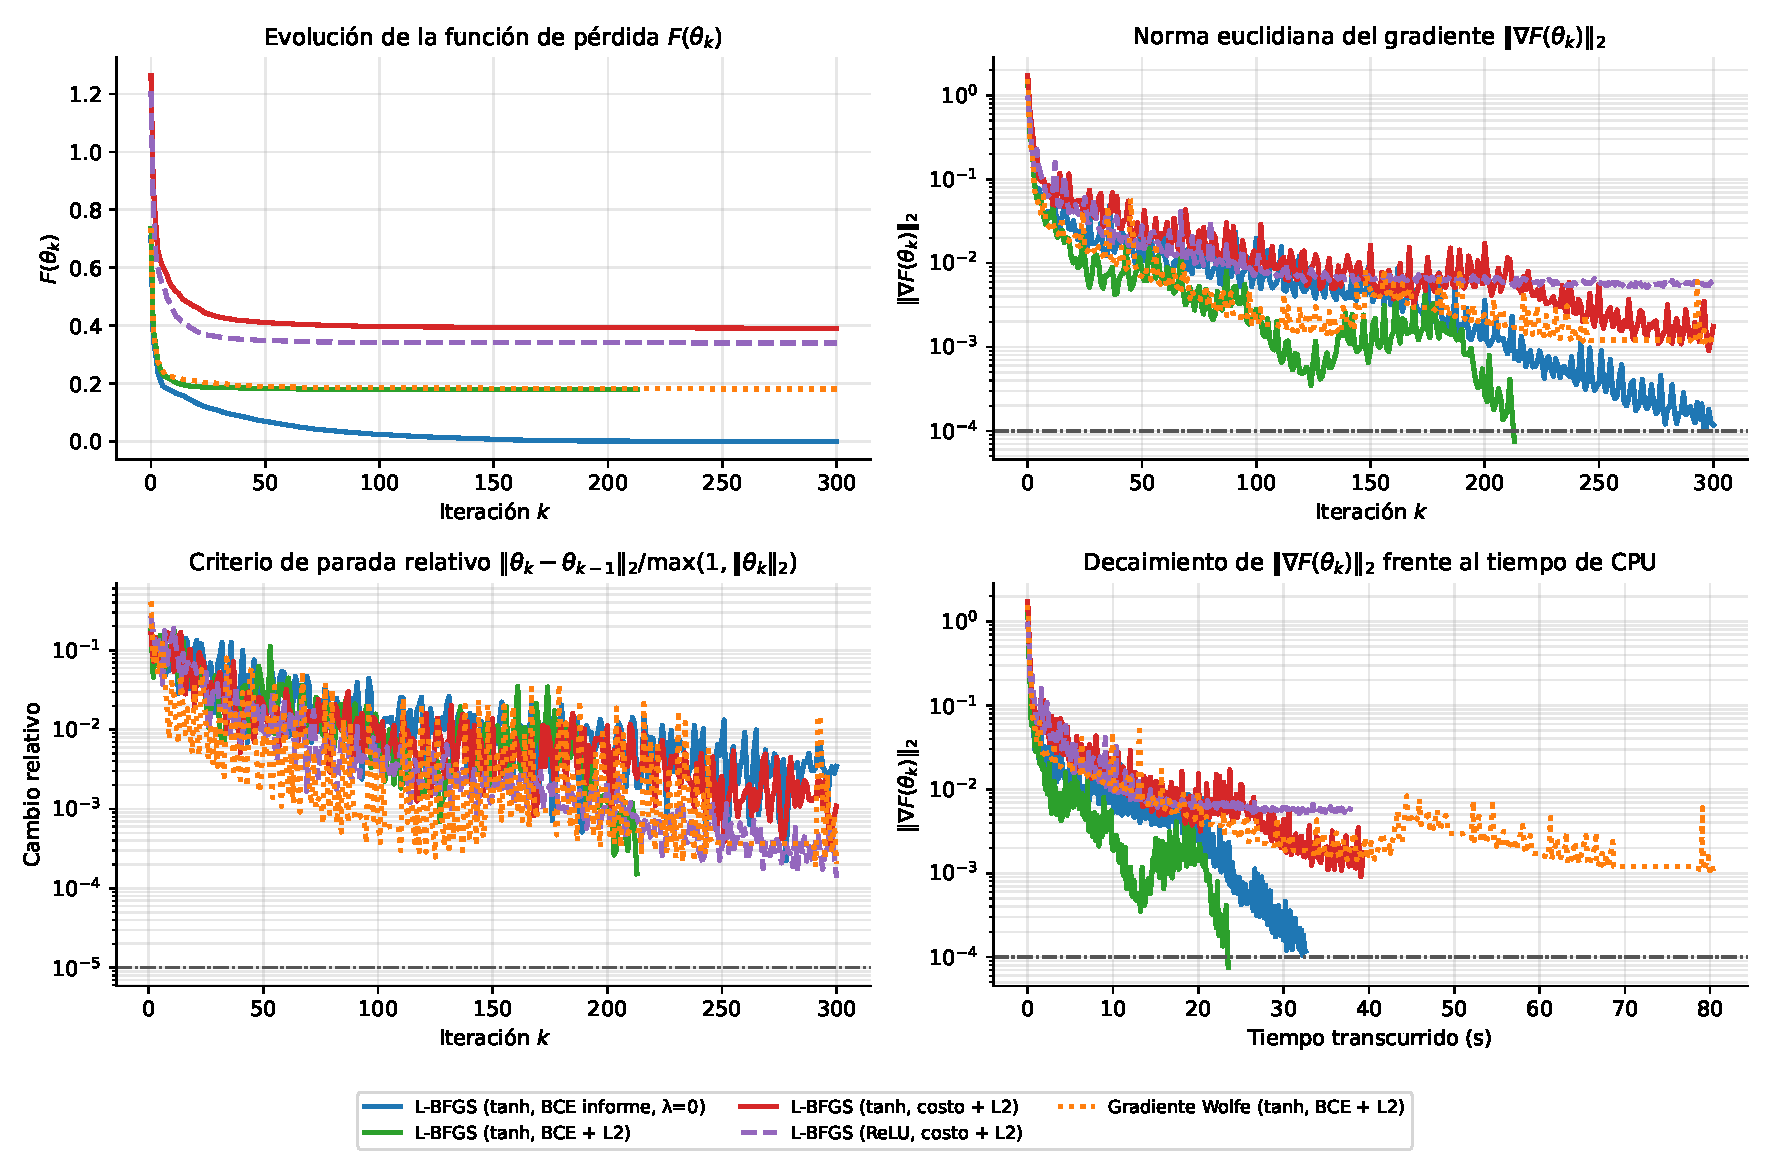
\includegraphics[width=\textwidth]{lbfgs_elliptic_convergencia.pdf}
\caption{Convergencia de L-BFGS frente al método del gradiente con búsqueda lineal de Wolfe sobre el dataset real Elliptic ($203\,769$ nodos): evolución de $F(\theta_k)$, norma del gradiente $\|\nabla F(\theta_k)\|_2$, paso relativo y tiempo de CPU.}
\label{fig:lbfgs-elliptic-convergencia}
\end{figure}

\begin{figure}[H]
\centering
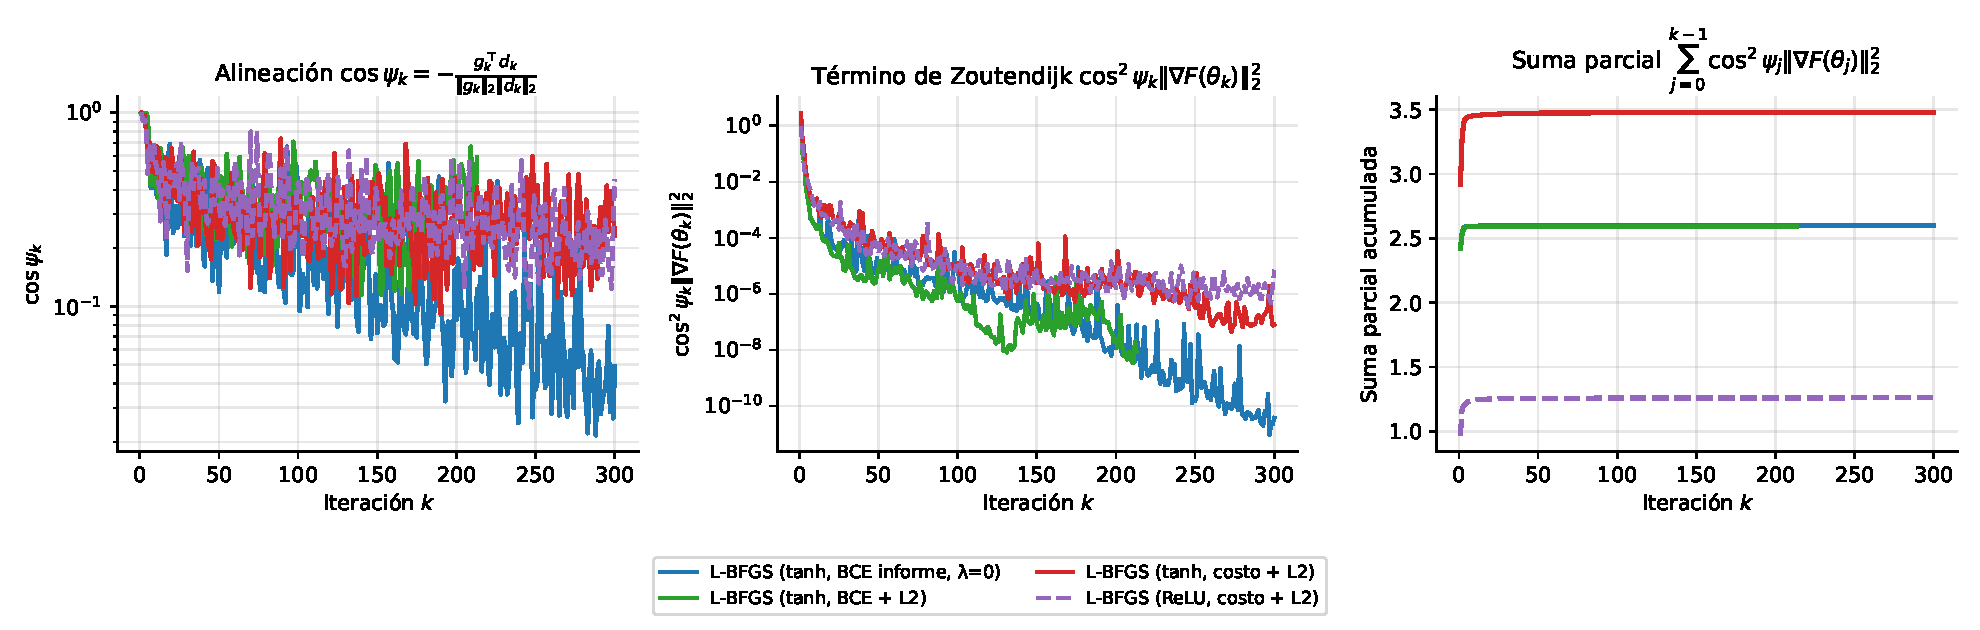
\includegraphics[width=\textwidth]{lbfgs_elliptic_zoutendijk.pdf}
\caption{Verificación numérica del Teorema~\ref{thm:zoutendijk} y del Corolario~\ref{cor:convergencia-global-limite} en Elliptic: evolución de $\cos\psi_k$, decaimiento del término $\cos^2\psi_k\|\nabla F(\theta_k)\|_2^2$ y estabilización de la suma parcial acumulada.}
\label{fig:lbfgs-elliptic-zoutendijk}
\end{figure}

\begin{table}[H]
\centering
\renewcommand{\arraystretch}{1.18}
\caption{Desempeño predictivo temporal en Elliptic (umbral elegido por máximo $F_1$ en validación, pasos 35--39; evaluación en prueba, pasos 40--49).}
\label{tab:lbfgs-elliptic-metricas}
\small
\resizebox{\linewidth}{!}{%
\begin{tabular}{lrrrrrr}
\toprule
\textbf{Configuración} & \textbf{Val PR-AUC} & \textbf{Val $F_1$} & \textbf{Test PR-AUC} & \textbf{Test $F_1$} & \textbf{Precisión} & \textbf{Exhaustividad} \\
\midrule
L-BFGS ($\tanh$, BCE, $\lambda=0$) & 0,5603 & 0,5638 & 0,2467 & 0,3076 & 0,2619 & 0,3726 \\
L-BFGS ($\tanh$, BCE + L2) & 0,5488 & 0,5677 & 0,3435 & 0,3534 & 0,2867 & 0,4607 \\
L-BFGS ($\tanh$, costo + L2) & 0,6405 & 0,6563 & 0,4083 & 0,4465 & 0,4345 & 0,4591 \\
L-BFGS ($\operatorname{ReLU}$, costo + L2) & 0,7550 & 0,7388 & 0,4509 & 0,4833 & 0,6771 & 0,3758 \\
Gradiente Wolfe ($\tanh$, BCE + L2) & 0,5433 & 0,5886 & 0,3309 & 0,3589 & 0,2947 & 0,4591 \\
\midrule
SciPy L-BFGS-B ($\tanh$, BCE + L2) & --- & --- & 0,3506 & 0,3690 & 0,3129 & 0,4497 \\
\bottomrule
\end{tabular}%
}
\end{table}

\begin{figure}[H]
\centering
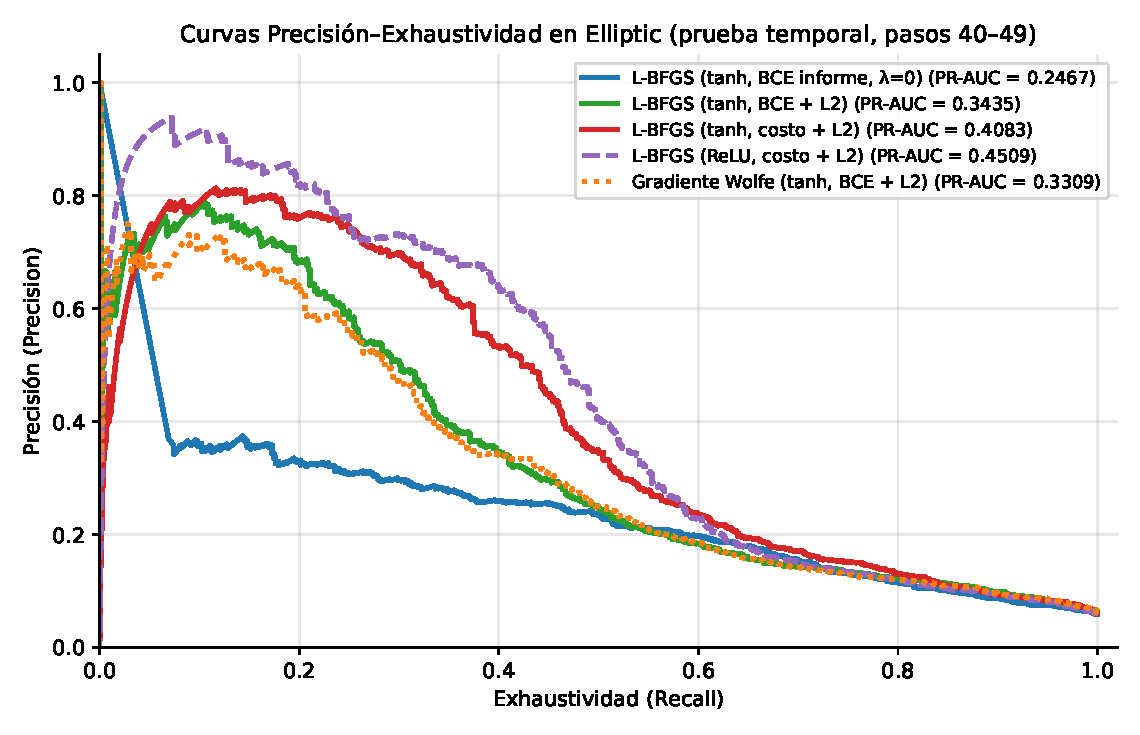
\includegraphics[width=0.82\textwidth]{lbfgs_elliptic_pr_curvas.pdf}
\caption{Curvas Precisión--Exhaustividad sobre los pasos temporales de prueba ($40$--$49$) en el conjunto de datos real Elliptic.}
\label{fig:lbfgs-elliptic-pr}
\end{figure}

\paragraph{Discusión de resultados.}
Los cuadros~\ref{tab:lbfgs-elliptic-opt}--\ref{tab:lbfgs-elliptic-metricas} y
las figuras~\ref{fig:lbfgs-elliptic-convergencia}--\ref{fig:lbfgs-elliptic-pr}
permiten extraer cuatro conclusiones verificables:
\begin{enumerate}
\item \textbf{Convergencia real y eficiencia de L-BFGS:} sobre la pérdida suave
y regularizada ($\tanh$, BCE + L2), el algoritmo L-BFGS de dos bucles satisface
el criterio de estacionariedad $\|\nabla F(\theta_k)\|_2\le 10^{-4}$ en $213$
iteraciones ($227$ evaluaciones, $23{,}50\,$s, con cero reinicios de memoria y
cero fallos de Wolfe), reduciendo en $3{,}4\times$ el tiempo y en $3{,}0\times$
las evaluaciones frente al método del gradiente con Wolfe ($80{,}36\,$s, $686$
evaluaciones, sin alcanzar la tolerancia). La validación cruzada con
\texttt{SciPy L-BFGS-B} confirma una trayectoria equivalente ($F_{\mathrm{fin}}=0{,}1802$
al detenerse por norma $\|g_k\|_\infty\le 10^{-4}$).
\item \textbf{Contraste directo con el Teorema~\ref{thm:zoutendijk}:} en todas
las corridas de L-BFGS el término de Zoutendijk $\cos^2\psi_k\|g_k\|_2^2$ decae
varios órdenes de magnitud y la suma parcial se estabiliza en un valor finito
($2{,}595$--$3{,}477$ con $\tanh$; $1{,}259$ con $\operatorname{ReLU}$). Sin
regularización ($\lambda=0$), L-BFGS lleva $F(\theta_k)$ desde $0{,}7045$ hasta
$1{,}07\times 10^{-4}$ en $32{,}56\,$s, pero el conjunto de nivel deja de ser
acotado y $\cos\psi_k$ desciende hasta $0{,}0216$, evidenciando mal
condicionamiento progresivo y sobreajuste temporal (PR-AUC en prueba $0{,}2467$).
Con regularización L2 ($\lambda=5\times 10^{-3}$), $\cos\psi_k$ se mantiene
acotado inferiormente por encima de $0{,}09$--$0{,}11$ y la generalización en
prueba aumenta notablemente (PR-AUC $0{,}3435$--$0{,}4509$).
\item \textbf{Efecto de la no diferenciabilidad de $\operatorname{ReLU}$:} con
$\operatorname{ReLU}$ y ponderación por costos se obtiene el mejor desempeño
predictivo temporal (Val PR-AUC $0{,}7550$, Test PR-AUC $0{,}4509$, Test $F_1=0{,}4833$,
precisión $67{,}71$\%), pero $\|\nabla F(\theta_k)\|_2$ se estanca en una
meseta alrededor de $6{,}1\times 10^{-3}$ pese a que el paso relativo baja a
$1{,}36\times 10^{-4}$, comportamiento típico de los quiebres no diferenciables
de $\operatorname{ReLU}$, donde falla la hipótesis de clase $C^1$ del
Teorema~\ref{thm:zoutendijk}. En cambio, con $\tanh$ ($C^\infty$) la norma del
gradiente desciende limpiamente hasta $7{,}48\times 10^{-5}$.
\item \textbf{Impacto del desbalance de clases:} incorporar el peso balanceado
$\omega_1=7{,}635$ ($\omega_0=1$) junto con $\lambda=5\times 10^{-3}$ eleva el PR-AUC de prueba con
$\tanh$ de $0{,}3435$ a $0{,}4083$ (y $F_1$ de $0{,}3534$ a $0{,}4465$),
confirmando su utilidad práctica en detección de fraude.
\end{enumerate}

% review_pending: corrida con tope de 1000 iteraciones (codigo/gcn_elliptic_lbfgs.py
% --max-iter 1000 --sufijo _1000, semilla 42); datos en
% resultados/resultados_elliptic_lbfgs_1000.json y resultados/historial_elliptic_1000/.
\paragraph{Extensión del tope a $1000$ iteraciones.}
Para distinguir las corridas detenidas por el tope de aquellas que no satisfacen
el criterio de estacionariedad, se repitió el experimento con idéntico
$\theta_0$ y un tope de $1000$ iteraciones
(Cuadro~\ref{tab:lbfgs-elliptic-opt-1000}).

\begin{table}[H]
\centering
\renewcommand{\arraystretch}{1.18}
\caption{Convergencia numérica en Elliptic con tope de $1000$ iteraciones (mismo $\theta_0$, memoria $M=10$).}
\label{tab:lbfgs-elliptic-opt-1000}
\small
\resizebox{\linewidth}{!}{%
\begin{tabular}{lrrrrrrl}
\toprule
\textbf{Configuración} & \textbf{Iters} & \textbf{Evals} & \textbf{Tiempo (s)} & $F_{\mathrm{fin}}$ & $\|\nabla F_{\mathrm{fin}}\|_2$ & \textbf{Test PR-AUC} & \textbf{Parada} \\
\midrule
L-BFGS ($\tanh$, BCE, $\lambda=0$) & 306 & 326 & 32,55 & 0,000099 & $9{,}21\times 10^{-5}$ & 0,2505 & $\|g_k\|_2\le 10^{-4}$ \\
L-BFGS ($\tanh$, BCE + L2) & 213 & 227 & 22,38 & 0,179115 & $7{,}48\times 10^{-5}$ & 0,3435 & $\|g_k\|_2\le 10^{-4}$ \\
L-BFGS ($\tanh$, costo + L2) & 570 & 610 & 60,53 & 0,390933 & $8{,}62\times 10^{-5}$ & 0,4093 & $\|g_k\|_2\le 10^{-4}$ \\
L-BFGS ($\operatorname{ReLU}$, costo + L2) & 960 & 965 & 77,21 & 0,339712 & $4{,}97\times 10^{-3}$ & 0,4454 & Paso rel.\ $\le 10^{-5}$ \\
Gradiente Wolfe ($\tanh$, BCE + L2) & 1000 & 2265 & 230,62 & 0,180387 & $4{,}10\times 10^{-4}$ & 0,3518 & Tope \\
\bottomrule
\end{tabular}%
}
\end{table}

Con $\tanh$, las tres corridas de L-BFGS satisfacen
$\|\nabla F(\theta_k)\|_2\le 10^{-4}$. En la configuración con costo y L2, que
con tope de $300$ quedaba en $1{,}76\times 10^{-3}$, la norma del gradiente
toma los valores $8{,}30\times 10^{-3}$, $1{,}76\times 10^{-3}$,
$6{,}78\times 10^{-4}$ y $8{,}62\times 10^{-5}$ en $k=100$, $300$, $500$ y
$570$. Con $\operatorname{ReLU}$ la norma del gradiente permanece en torno a
$5\times 10^{-3}$ desde $k\approx 300$ y la corrida se detiene por paso
relativo, no por estacionariedad. El método del gradiente no alcanza la
tolerancia en $1000$ iteraciones ($230{,}62\,$s), mientras que L-BFGS lo logra
sobre la misma función en $213$ iteraciones ($22{,}38\,$s). En la corrida sin
regularización la parada por gradiente no indica proximidad a un minimizador:
como el ínfimo $0$ de $F$ no se alcanza, $\|\nabla F(\theta_k)\|_2$ puede
tender a cero sin que $(\theta_k)$ converja.
% review_pending: la divergencia de \|\theta_k\| con \lambda=0 es conjetura; no se midió \|\theta_k\|.

% Procedencia: experimento adicional Nivel 2 (IA, Antigravity, 2026-11-24;
% codigo/gcn_elliptic_nivel2.py y resultados/resultados_elliptic_nivel2.json),
% tope 300 iteraciones. review_pending.
\paragraph{Contraste entre óptimo global convexo ($L_{\mathrm{net}}=1$), arquitectura ego-separada ($L_{\mathrm{net}}=2$) y suavización $\operatorname{softplus}_\beta$ con \emph{multi-start}.}
Con el fin de evaluar directamente la Proposición~\ref{prop:convexidad-una-capa-vs-simetria} usando la arquitectura polinomial exacta sin sesgos de la Definición~\ref{def:gcnn-red} y el conteo de parámetros de la Proposición~\ref{prop:gcnn-parametros} ($\omega_1\approx 7{,}635$, $\omega_0=1$, $\lambda=5\times 10^{-3}$, memoria $M=10$ y tope de $300$ iteraciones; \texttt{gcn\_elliptic\_nivel2.py}), se ejecutaron tres regímenes adicionales cuyos gradientes analíticos se verificaron contra diferencias finitas centrales ($\varepsilon=10^{-6}$, error relativo máximo $6{,}57\times 10^{-8}$ en $L_{\mathrm{net}}=1$ y $\le 6{,}12\times 10^{-6}$ en $L_{\mathrm{net}}=2$):
\begin{enumerate}
\item \textbf{Modelo FIR convexo de óptimo global ($L_{\mathrm{net}}=1$, $K_1=2$, $p=3\times 165=495$):} precalculando $\widetilde{X}_{34}=[X,S_{34}X,S_{34}^2X]$, se obtiene $\|\widetilde{X}_{I_{\mathrm{tr}}}\|_2=2\,113{,}33$ y constante Lipschitz global exacta $L=285{,}17$ ($\kappa\le L/\lambda\approx 5{,}70\times 10^4$). L-BFGS alcanza $\|\nabla F_{\omega,\lambda}(\theta_k)\|_2=9{,}58\times 10^{-5}\le 10^{-4}$ en solo $79$ iteraciones ($3{,}32\,$s). Para verificar empíricamente la unicidad del minimizador global $\theta^*$, se repitió la corrida desde $\theta_0=0$ ($77$ iteraciones, $3{,}45\,$s), obteniéndose $|F_{\omega,\lambda}(\hat\theta_{\mathrm{aleat}})-F_{\omega,\lambda}(\hat\theta_0)|=6{,}93\times 10^{-9}$ y $\|\hat\theta_{\mathrm{aleat}}-\hat\theta_0\|_2=4{,}89\times 10^{-3}$. Sin embargo, en dicho único mínimo global el desempeño predictivo temporal se limita a Test PR-AUC $0{,}1725$ ($F_1=0{,}2835$), probando empíricamente que las combinaciones no lineales de una capa oculta ($L_{\mathrm{net}}=2$) son indispensables en detección de fraude.
\item \textbf{GCNN ego-separada ($L_{\mathrm{net}}=2$, $K_1=K_2=1$, $d_1=32$, $p=2\cdot 165\cdot 32+2\cdot 32=10\,624$):} al separar los pesos del propio vértice ($X W_0^{(1)}$) de los de su vecindad ($S_t X W_1^{(1)}$) para evitar diluir atributos bajo heterofilia, el valor objetivo desciende de $0{,}3910$ (\texttt{ExplicitGCN}) a $0{,}2067$ con $\tanh$ y a $0{,}2010$--$0{,}2020$ con $\operatorname{softplus}_2$ ($\beta=2$, error uniforme $\frac{\log 2}{2}\approx 0{,}3466$ frente a $\operatorname{ReLU}$). Sobre la misma semilla $42$, sustituir $\tanh$ por $\operatorname{softplus}_2$ evita la saturación positiva y eleva el Val PR-AUC de $0{,}6799$ a $0{,}7401$ y el Test PR-AUC de $0{,}3335$ a $0{,}3964$.
\item \textbf{Exploración de cuencas locales mediante \emph{multi-start} ($R=5$ semillas $42$--$46$) y ensamblado:} las cinco corridas independientes con $\operatorname{softplus}_2$ convergen hacia cuencas locales geométricamente separadas ($\|\hat\theta^{(r)}-\hat\theta^{(s)}\|_2\in[8{,}16;\,9{,}09]$, frente a $4{,}89\times 10^{-3}$ en el modelo convexo), todas con valores objetivos casi equivalentes ($F_{\mathrm{fin}}\in[0{,}201041;\,0{,}202032]$) y Test $F_1$ individual de hasta $0{,}5128$ (semilla $45$). El ensamble promedio $\bar p_i=\frac15\sum_{r=1}^5 p_i(\hat\theta^{(r)})$ alcanza el mayor PR-AUC de validación de todo el estudio ($0{,}7594$) y eleva el puntaje $F_1$ en prueba temporal a $0{,}5023$ (precisión $60{,}22$\%, exhaustividad $43{,}08$\%), superando en $F_1$ a todas las variantes de un solo modelo del Cuadro~\ref{tab:lbfgs-elliptic-metricas}.
\end{enumerate}

\begin{table}[H]
\centering
\renewcommand{\arraystretch}{1.18}
\caption{Comparación en Elliptic (tope de $300$ iteraciones, $\omega_1\approx 7{,}635$, $\lambda=5\times 10^{-3}$) entre el óptimo global convexo ($L_{\mathrm{net}}=1$) y la GCNN ego-separada ($L_{\mathrm{net}}=2$, Definición~\ref{def:gcnn-red}) con $\operatorname{softplus}_2$ y \emph{multi-start}.}
\label{tab:lbfgs-elliptic-nivel2}
\small
\resizebox{\linewidth}{!}{%
\begin{tabular}{lrrrrrrrrr}
\toprule
\textbf{Arquitectura y régimen} & $p$ & \textbf{Iters} & \textbf{Tiempo (s)} & $F_{\mathrm{fin}}$ & $\|\nabla F_{\mathrm{fin}}\|_2$ & \textbf{Val PR-AUC} & \textbf{Test PR-AUC} & \textbf{Test $F_1$} & \textbf{Precisión} \\
\midrule
FIR convexo ($L_{\mathrm{net}}=1, K_1=2$, óptimo global) & 495 & 79 & 3,32 & 0,425522 & $9{,}58\times 10^{-5}$ & 0,3291 & 0,1725 & 0,2835 & 0,1915 \\
GCNN ego-sep.\ ($L_{\mathrm{net}}=2, K_\ell=1$, $\tanh$, s42) & 10\,624 & 300 & 244,20 & 0,206731 & $3{,}05\times 10^{-3}$ & 0,6799 & 0,3335 & 0,4766 & 0,4662 \\
GCNN ego-sep.\ ($L_{\mathrm{net}}=2, K_\ell=1$, $\operatorname{softplus}_2$, s42) & 10\,624 & 300 & 313,29 & 0,201041 & $2{,}45\times 10^{-3}$ & 0,7401 & 0,3964 & 0,4829 & 0,5865 \\
GCNN ego-sep.\ ($\operatorname{softplus}_2$, mejor val.\ s44) & 10\,624 & 300 & 177,21 & 0,201577 & $7{,}10\times 10^{-3}$ & 0,7480 & 0,3850 & 0,5014 & 0,5935 \\
GCNN ego-sep.\ ($\operatorname{softplus}_2$, s45 máx.\ Test) & 10\,624 & 300 & 192,92 & 0,201833 & $2{,}36\times 10^{-3}$ & 0,7066 & 0,4159 & 0,5128 & 0,5832 \\
\midrule
Ensamble \emph{multi-start} ($R=5$, $\operatorname{softplus}_2$) & $5\times 10\,624$ & $5\times 300$ & 982,33 & --- & --- & \textbf{0,7594} & 0,4022 & \textbf{0,5023} & 0,6022 \\
\bottomrule
\end{tabular}%
}
\end{table}

\appendix

% Historiales generados por codigo/gcn_elliptic_lbfgs.py (semilla 42): --max-iter 300
% (resultados/historial_elliptic/) y --max-iter 1000 --sufijo _1000
% (resultados/historial_elliptic_1000/). Valores redondeados a 12 decimales
% (F en coma fija; la norma del gradiente, en notación científica). review_pending
\chapter{Historial de iteraciones de la experimentación en Elliptic}
\label{app:historial-elliptic}

El Cuadro~\ref{tab:lbfgs-elliptic-historial} recoge, para cada iteración $k\in\{0,\ldots,1000\}$, el valor de la función objetivo $F_{\omega,\lambda}(\theta_k)$ (abreviada como $F(\theta_k)$) y la norma del gradiente $\|\nabla F(\theta_k)\|_2$ en las cinco configuraciones de los cuadros~\ref{tab:lbfgs-elliptic-opt} y~\ref{tab:lbfgs-elliptic-opt-1000}, todas iniciadas en el mismo $\theta_0$ (semilla $42$); los valores se redondean a $12$ decimales ($F(\theta_k)$ en coma fija y $\|\nabla F(\theta_k)\|_2$ en notación científica).
Dado que ambas corridas comparten exactamente la misma trayectoria hasta $k=300$, se presentan en un único cuadro continuo con una línea divisoria tras $k=300$ que señala el corte del experimento base (Cuadro~\ref{tab:lbfgs-elliptic-opt}): en dicho corte la configuración (ii) ya se había detenido en $k=213$ al cumplirse $\|\nabla F(\theta_k)\|_2\le 10^{-4}$, mientras que al extender el tope a $1000$ iteraciones (Cuadro~\ref{tab:lbfgs-elliptic-opt-1000}) las configuraciones (i) y (iii) alcanzan también $\|\nabla F(\theta_k)\|_2\le 10^{-4}$ en $k=306$ y $k=570$, (iv) se detiene por paso relativo en $k=960$ y (v) alcanza $k=1000$.
\begin{landscape}
{\fontsize{4.6pt}{5.2pt}\selectfont
\setlength{\tabcolsep}{2.5pt}
\setlength{\LTcapwidth}{\textwidth}
\begin{longtable}{r*{10}{r}}
\caption{Historial completo de $F(\theta_k)$ y $\|\nabla F(\theta_k)\|_2$ en Elliptic (memoria $M=10$, $k=0,\ldots,1000$; la línea horizontal tras $k=300$ marca el corte del Cuadro~\ref{tab:lbfgs-elliptic-opt}).}
\label{tab:lbfgs-elliptic-historial}\label{tab:lbfgs-elliptic-historial-1000}\\
\toprule
\multicolumn{1}{c}{} & \multicolumn{2}{c}{\textbf{(i)} $\tanh$, BCE, $\lambda=0$} & \multicolumn{2}{c}{\textbf{(ii)} $\tanh$, BCE + L2} & \multicolumn{2}{c}{\textbf{(iii)} $\tanh$, costo + L2} & \multicolumn{2}{c}{\textbf{(iv)} $\operatorname{ReLU}$, costo + L2} & \multicolumn{2}{c}{\textbf{(v)} Gradiente, BCE + L2} \\
\cmidrule(lr){2-3}\cmidrule(lr){4-5}\cmidrule(lr){6-7}\cmidrule(lr){8-9}\cmidrule(lr){10-11}
$k$ & $F(\theta_k)$ & $\|\nabla F(\theta_k)\|_2$ & $F(\theta_k)$ & $\|\nabla F(\theta_k)\|_2$ & $F(\theta_k)$ & $\|\nabla F(\theta_k)\|_2$ & $F(\theta_k)$ & $\|\nabla F(\theta_k)\|_2$ & $F(\theta_k)$ & $\|\nabla F(\theta_k)\|_2$ \\
\midrule
\endfirsthead
\multicolumn{11}{l}{\textit{Continuación del Cuadro~\ref{tab:lbfgs-elliptic-historial-1000}}}\\
\toprule
\multicolumn{1}{c}{} & \multicolumn{2}{c}{\textbf{(i)} $\tanh$, BCE, $\lambda=0$} & \multicolumn{2}{c}{\textbf{(ii)} $\tanh$, BCE + L2} & \multicolumn{2}{c}{\textbf{(iii)} $\tanh$, costo + L2} & \multicolumn{2}{c}{\textbf{(iv)} $\operatorname{ReLU}$, costo + L2} & \multicolumn{2}{c}{\textbf{(v)} Gradiente, BCE + L2} \\
\cmidrule(lr){2-3}\cmidrule(lr){4-5}\cmidrule(lr){6-7}\cmidrule(lr){8-9}\cmidrule(lr){10-11}
$k$ & $F(\theta_k)$ & $\|\nabla F(\theta_k)\|_2$ & $F(\theta_k)$ & $\|\nabla F(\theta_k)\|_2$ & $F(\theta_k)$ & $\|\nabla F(\theta_k)\|_2$ & $F(\theta_k)$ & $\|\nabla F(\theta_k)\|_2$ & $F(\theta_k)$ & $\|\nabla F(\theta_k)\|_2$ \\
\midrule
\endhead
\midrule
\multicolumn{11}{r}{\textit{Continúa en la página siguiente}}\\
\endfoot
\bottomrule
\endlastfoot
0 & 0,704450448372 & 1,555786108617·10\textsuperscript{0} & 0,735770085555 & 1,556062234995·10\textsuperscript{0} & 1,262528428648 & 1,707717621988·10\textsuperscript{0} & 1,207967219951 & 9,841975885814·10\textsuperscript{−1} & 0,735770085555 & 1,556062234995·10\textsuperscript{0} \\
1 & 0,352548483664 & 3,359522184354·10\textsuperscript{−1} & 0,384759253619 & 3,345631668264·10\textsuperscript{−1} & 0,883266145972 & 6,246753507128·10\textsuperscript{−1} & 0,813072172488 & 4,903191451500·10\textsuperscript{−1} & 0,389759484502 & 2,901998729134·10\textsuperscript{−1} \\
2 & 0,306963755641 & 2,334159993778·10\textsuperscript{−1} & 0,339814817529 & 2,317199770621·10\textsuperscript{−1} & 0,761586701466 & 3,754293746888·10\textsuperscript{−1} & 0,654342271321 & 1,968570649981·10\textsuperscript{−1} & 0,325245735561 & 1,888190416229·10\textsuperscript{−1} \\
3 & 0,239261147324 & 8,794403325615·10\textsuperscript{−2} & 0,274354105418 & 8,613324161332·10\textsuperscript{−2} & 0,658063271207 & 2,051927764468·10\textsuperscript{−1} & 0,600231063326 & 1,283871436329·10\textsuperscript{−1} & 0,275151164476 & 7,387557584550·10\textsuperscript{−2} \\
4 & 0,216251249872 & 5,955195389324·10\textsuperscript{−2} & 0,252850908362 & 5,776491257868·10\textsuperscript{−2} & 0,629067105518 & 1,942447214548·10\textsuperscript{−1} & 0,566457964316 & 2,283299680162·10\textsuperscript{−1} & 0,262746355416 & 5,967280508771·10\textsuperscript{−2} \\
5 & 0,193128383366 & 7,650929083370·10\textsuperscript{−2} & 0,231552072138 & 6,222389141387·10\textsuperscript{−2} & 0,606316291279 & 1,031826121591·10\textsuperscript{−1} & 0,541294632066 & 1,356574669745·10\textsuperscript{−1} & 0,248393099880 & 4,703033468813·10\textsuperscript{−2} \\
6 & 0,186369379702 & 5,450703604764·10\textsuperscript{−2} & 0,225819139424 & 5,602866717725·10\textsuperscript{−2} & 0,591090173119 & 9,401980228980·10\textsuperscript{−2} & 0,528174480321 & 1,065768377984·10\textsuperscript{−1} & 0,231064402104 & 3,648470950896·10\textsuperscript{−2} \\
7 & 0,183018285582 & 3,564902127387·10\textsuperscript{−2} & 0,221888254958 & 3,596681995410·10\textsuperscript{−2} & 0,575829800965 & 9,905542578324·10\textsuperscript{−2} & 0,495482839887 & 9,544497960309·10\textsuperscript{−2} & 0,228012915900 & 6,318975294466·10\textsuperscript{−2} \\
8 & 0,179384280102 & 2,950365230641·10\textsuperscript{−2} & 0,218000060261 & 2,854367616420·10\textsuperscript{−2} & 0,552561817574 & 6,873482072155·10\textsuperscript{−2} & 0,482459820399 & 6,313583482883·10\textsuperscript{−2} & 0,225712464058 & 2,990613688923·10\textsuperscript{−2} \\
9 & 0,175892955941 & 4,112741400528·10\textsuperscript{−2} & 0,213960372124 & 3,888607002016·10\textsuperscript{−2} & 0,537646829250 & 8,341949458703·10\textsuperscript{−2} & 0,465443044332 & 6,357510572311·10\textsuperscript{−2} & 0,224904927810 & 2,752942012482·10\textsuperscript{−2} \\
10 & 0,170965120526 & 4,070738191575·10\textsuperscript{−2} & 0,208241306395 & 3,517878036955·10\textsuperscript{−2} & 0,526964362178 & 7,545304488906·10\textsuperscript{−2} & 0,448263522593 & 6,047041936778·10\textsuperscript{−2} & 0,221166339218 & 2,585787786281·10\textsuperscript{−2} \\
11 & 0,165884353181 & 3,862106618180·10\textsuperscript{−2} & 0,203467089891 & 4,640523068054·10\textsuperscript{−2} & 0,518696350973 & 5,011161908317·10\textsuperscript{−2} & 0,432042065063 & 7,576112610025·10\textsuperscript{−2} & 0,219019856696 & 2,974240740917·10\textsuperscript{−2} \\
12 & 0,163201448617 & 4,775623619821·10\textsuperscript{−2} & 0,199912361705 & 2,618210623610·10\textsuperscript{−2} & 0,511693650694 & 4,920466379988·10\textsuperscript{−2} & 0,427225071884 & 1,593770072682·10\textsuperscript{−1} & 0,218095365679 & 2,372160222437·10\textsuperscript{−2} \\
13 & 0,160818561814 & 2,322907265405·10\textsuperscript{−2} & 0,198285138445 & 2,014296310492·10\textsuperscript{−2} & 0,500077150852 & 7,248564977842·10\textsuperscript{−2} & 0,417198134497 & 4,994036608763·10\textsuperscript{−2} & 0,217541532850 & 2,203682677685·10\textsuperscript{−2} \\
14 & 0,159224738977 & 2,356385885162·10\textsuperscript{−2} & 0,196461551084 & 2,177542694014·10\textsuperscript{−2} & 0,491433909491 & 1,181789840883·10\textsuperscript{−1} & 0,413820775163 & 4,769026645770·10\textsuperscript{−2} & 0,213894376203 & 2,305390648895·10\textsuperscript{−2} \\
15 & 0,153939145116 & 3,577514709439·10\textsuperscript{−2} & 0,194214104642 & 2,446081585481·10\textsuperscript{−2} & 0,484971488909 & 6,484286821837·10\textsuperscript{−2} & 0,405116775988 & 5,630092802785·10\textsuperscript{−2} & 0,213035575407 & 3,525261710772·10\textsuperscript{−2} \\
16 & 0,149226703310 & 4,834559726790·10\textsuperscript{−2} & 0,192600593907 & 1,748810580078·10\textsuperscript{−2} & 0,481159241340 & 4,716376482882·10\textsuperscript{−2} & 0,401312646923 & 1,079295976098·10\textsuperscript{−1} & 0,212304187304 & 1,902679616631·10\textsuperscript{−2} \\
17 & 0,145291935217 & 3,649611051788·10\textsuperscript{−2} & 0,191385799864 & 1,999538584466·10\textsuperscript{−2} & 0,475752985992 & 5,851348509099·10\textsuperscript{−2} & 0,394902187840 & 6,336969040906·10\textsuperscript{−2} & 0,211086262167 & 1,893328567450·10\textsuperscript{−2} \\
18 & 0,141776738372 & 2,571202401163·10\textsuperscript{−2} & 0,190649643593 & 1,952966911656·10\textsuperscript{−2} & 0,471089037514 & 1,156345125536·10\textsuperscript{−1} & 0,389727319272 & 4,014524797823·10\textsuperscript{−2} & 0,210482283575 & 1,869305310996·10\textsuperscript{−2} \\
19 & 0,137548380072 & 2,528934904477·10\textsuperscript{−2} & 0,189949995074 & 1,201376901105·10\textsuperscript{−2} & 0,465872379634 & 5,687555425499·10\textsuperscript{−2} & 0,384961648864 & 4,264950559459·10\textsuperscript{−2} & 0,210156021738 & 1,762409671645·10\textsuperscript{−2} \\
20 & 0,132757154872 & 3,198772943736·10\textsuperscript{−2} & 0,189367010645 & 1,003170656797·10\textsuperscript{−2} & 0,463407040170 & 4,720943575568·10\textsuperscript{−2} & 0,379871990210 & 4,069078809700·10\textsuperscript{−2} & 0,208087371582 & 1,952234617208·10\textsuperscript{−2} \\
21 & 0,128289564513 & 2,302263519045·10\textsuperscript{−2} & 0,188746661057 & 1,123475656104·10\textsuperscript{−2} & 0,458954771092 & 5,358573460748·10\textsuperscript{−2} & 0,377327871619 & 4,949201941167·10\textsuperscript{−2} & 0,207633222523 & 2,130991199886·10\textsuperscript{−2} \\
22 & 0,125931095826 & 1,908738276551·10\textsuperscript{−2} & 0,188120607744 & 8,799075773098·10\textsuperscript{−3} & 0,452711883834 & 5,565969700822·10\textsuperscript{−2} & 0,373805070917 & 3,832306455014·10\textsuperscript{−2} & 0,207347145097 & 1,604232680061·10\textsuperscript{−2} \\
23 & 0,121506085890 & 2,388395565852·10\textsuperscript{−2} & 0,187698005133 & 9,290715207992·10\textsuperscript{−3} & 0,447315013301 & 5,508130408973·10\textsuperscript{−2} & 0,371104914693 & 3,814389339004·10\textsuperscript{−2} & 0,204269579740 & 1,593761477003·10\textsuperscript{−2} \\
24 & 0,118829310529 & 2,287232271278·10\textsuperscript{−2} & 0,187398652740 & 2,050668670210·10\textsuperscript{−2} & 0,443025331719 & 4,511372599113·10\textsuperscript{−2} & 0,368454506110 & 3,988018197769·10\textsuperscript{−2} & 0,203650135372 & 4,061558669198·10\textsuperscript{−2} \\
25 & 0,116597819765 & 1,705799437424·10\textsuperscript{−2} & 0,187150841538 & 1,138651896406·10\textsuperscript{−2} & 0,440374248005 & 3,587471833314·10\textsuperscript{−2} & 0,367108649046 & 6,105641738830·10\textsuperscript{−2} & 0,202740785868 & 1,665241437751·10\textsuperscript{−2} \\
26 & 0,114332207323 & 1,421695752214·10\textsuperscript{−2} & 0,187027039314 & 6,782732048738·10\textsuperscript{−3} & 0,437595654151 & 4,957439735995·10\textsuperscript{−2} & 0,365519627673 & 3,026116893966·10\textsuperscript{−2} & 0,202536345563 & 1,371788090225·10\textsuperscript{−2} \\
27 & 0,112318685284 & 3,919459393076·10\textsuperscript{−2} & 0,186837249026 & 5,136122575877·10\textsuperscript{−3} & 0,435550980185 & 7,400121652198·10\textsuperscript{−2} & 0,364525918129 & 3,061433389839·10\textsuperscript{−2} & 0,201996154219 & 1,501700638390·10\textsuperscript{−2} \\
28 & 0,110155736396 & 1,719654584644·10\textsuperscript{−2} & 0,186631242377 & 6,786652326528·10\textsuperscript{−3} & 0,433252955297 & 4,188964793188·10\textsuperscript{−2} & 0,362771967763 & 3,724983047295·10\textsuperscript{−2} & 0,201820991215 & 1,327935604174·10\textsuperscript{−2} \\
29 & 0,108876682231 & 1,719464918671·10\textsuperscript{−2} & 0,186411513787 & 1,177026912213·10\textsuperscript{−2} & 0,431367079109 & 3,523072207170·10\textsuperscript{−2} & 0,361641899800 & 5,746065092946·10\textsuperscript{−2} & 0,201333885061 & 1,419901631259·10\textsuperscript{−2} \\
30 & 0,105651021201 & 1,793342233504·10\textsuperscript{−2} & 0,186227897803 & 1,248729205408·10\textsuperscript{−2} & 0,429125287430 & 3,520569480725·10\textsuperscript{−2} & 0,360277213699 & 3,352579922359·10\textsuperscript{−2} & 0,201177703196 & 1,288741583270·10\textsuperscript{−2} \\
31 & 0,102342962222 & 1,931684872850·10\textsuperscript{−2} & 0,186118418492 & 1,004618369288·10\textsuperscript{−2} & 0,427043834973 & 6,020466413248·10\textsuperscript{−2} & 0,359207271569 & 2,638975183081·10\textsuperscript{−2} & 0,200273416812 & 1,571047820451·10\textsuperscript{−2} \\
32 & 0,099890962984 & 3,004478759962·10\textsuperscript{−2} & 0,186062465072 & 5,805542567618·10\textsuperscript{−3} & 0,425852305528 & 6,821645768776·10\textsuperscript{−2} & 0,358335933530 & 2,332338229113·10\textsuperscript{−2} & 0,200095556351 & 1,294040907062·10\textsuperscript{−2} \\
33 & 0,097877589289 & 1,388706332858·10\textsuperscript{−2} & 0,186005113434 & 5,023220642275·10\textsuperscript{−3} & 0,424581092109 & 2,730052224957·10\textsuperscript{−2} & 0,357224367789 & 2,114110096113·10\textsuperscript{−2} & 0,199984179464 & 1,223042489316·10\textsuperscript{−2} \\
34 & 0,096492641093 & 1,276851769969·10\textsuperscript{−2} & 0,185891335249 & 6,997256146275·10\textsuperscript{−3} & 0,423830037583 & 2,966321540119·10\textsuperscript{−2} & 0,356233793510 & 3,418094727152·10\textsuperscript{−2} & 0,196793551778 & 1,082583103949·10\textsuperscript{−2} \\
35 & 0,094606298592 & 1,226125025003·10\textsuperscript{−2} & 0,185765143721 & 7,219972470031·10\textsuperscript{−3} & 0,422836466134 & 3,726945822546·10\textsuperscript{−2} & 0,355565047754 & 3,770159512309·10\textsuperscript{−2} & 0,195859384593 & 4,763367655565·10\textsuperscript{−2} \\
36 & 0,093798772170 & 4,903945898429·10\textsuperscript{−2} & 0,185556956313 & 7,622341229227·10\textsuperscript{−3} & 0,420985457742 & 3,984381846871·10\textsuperscript{−2} & 0,354905460810 & 1,895484095374·10\textsuperscript{−2} & 0,195026439928 & 1,325185808416·10\textsuperscript{−2} \\
37 & 0,090841772528 & 1,624872332135·10\textsuperscript{−2} & 0,185482933072 & 8,924434794059·10\textsuperscript{−3} & 0,420114482871 & 6,906212519802·10\textsuperscript{−2} & 0,354354406378 & 1,576308290067·10\textsuperscript{−2} & 0,194933051483 & 9,755629595427·10\textsuperscript{−3} \\
38 & 0,089607756113 & 1,353494621872·10\textsuperscript{−2} & 0,185373860033 & 4,236938997455·10\textsuperscript{−3} & 0,418324814311 & 4,276960008802·10\textsuperscript{−2} & 0,353766417455 & 3,048993670880·10\textsuperscript{−2} & 0,194448915421 & 1,199754828288·10\textsuperscript{−2} \\
39 & 0,088003039130 & 1,954815458114·10\textsuperscript{−2} & 0,185305748443 & 4,354418820420·10\textsuperscript{−3} & 0,417931800413 & 6,239224132847·10\textsuperscript{−2} & 0,353403358630 & 3,557280243760·10\textsuperscript{−2} & 0,194331230928 & 9,701766074186·10\textsuperscript{−3} \\
40 & 0,086325235246 & 1,618402295254·10\textsuperscript{−2} & 0,185195461754 & 6,491740937071·10\textsuperscript{−3} & 0,417318711205 & 2,669529140323·10\textsuperscript{−2} & 0,352985034726 & 1,979272422837·10\textsuperscript{−2} & 0,194256422130 & 9,317084364818·10\textsuperscript{−3} \\
41 & 0,084525373738 & 2,427396091640·10\textsuperscript{−2} & 0,185063767610 & 7,442624771635·10\textsuperscript{−3} & 0,416893878736 & 2,570972637993·10\textsuperscript{−2} & 0,352651680782 & 1,815809309854·10\textsuperscript{−2} & 0,193392805581 & 1,552140270821·10\textsuperscript{−2} \\
42 & 0,082356084634 & 2,103452175402·10\textsuperscript{−2} & 0,184925478682 & 7,590538429970·10\textsuperscript{−3} & 0,416318762089 & 3,207588660040·10\textsuperscript{−2} & 0,352360406446 & 2,302777609155·10\textsuperscript{−2} & 0,193281109117 & 1,051785153051·10\textsuperscript{−2} \\
43 & 0,081192607499 & 1,512539354333·10\textsuperscript{−2} & 0,184861398746 & 1,574605346017·10\textsuperscript{−2} & 0,415360404372 & 3,304061971315·10\textsuperscript{−2} & 0,351889736131 & 2,190997380460·10\textsuperscript{−2} & 0,193222191431 & 8,713824878097·10\textsuperscript{−3} \\
44 & 0,078567153553 & 1,343253019486·10\textsuperscript{−2} & 0,184745065052 & 7,786818539025·10\textsuperscript{−3} & 0,414728602952 & 5,482341150316·10\textsuperscript{−2} & 0,351342964877 & 1,633814210166·10\textsuperscript{−2} & 0,191767361014 & 8,128431205149·10\textsuperscript{−3} \\
45 & 0,077159721895 & 1,631462717618·10\textsuperscript{−2} & 0,184659532047 & 4,905007365613·10\textsuperscript{−3} & 0,413830730540 & 2,393410257727·10\textsuperscript{−2} & 0,350877494751 & 1,703822116127·10\textsuperscript{−2} & 0,191668002784 & 5,826132775962·10\textsuperscript{−2} \\
46 & 0,075293903616 & 1,388810411248·10\textsuperscript{−2} & 0,184552237699 & 5,384408098526·10\textsuperscript{−3} & 0,413385068852 & 1,956745009256·10\textsuperscript{−2} & 0,350403607160 & 2,007169588040·10\textsuperscript{−2} & 0,190448699728 & 2,389132033480·10\textsuperscript{−2} \\
47 & 0,073586620063 & 1,029212309105·10\textsuperscript{−2} & 0,184384657063 & 7,075532623142·10\textsuperscript{−3} & 0,412774845633 & 2,293722057529·10\textsuperscript{−2} & 0,349900014059 & 1,945588164565·10\textsuperscript{−2} & 0,190247859172 & 9,251608562363·10\textsuperscript{−3} \\
48 & 0,071887122062 & 9,406453621777·10\textsuperscript{−3} & 0,184142092156 & 9,256571356873·10\textsuperscript{−3} & 0,412010140506 & 3,025169353146·10\textsuperscript{−2} & 0,349464802391 & 1,558292702639·10\textsuperscript{−2} & 0,190201394960 & 7,760448103396·10\textsuperscript{−3} \\
49 & 0,071169544830 & 2,364960466011·10\textsuperscript{−2} & 0,183960244673 & 1,160700693776·10\textsuperscript{−2} & 0,411278118465 & 2,229379816894·10\textsuperscript{−2} & 0,349124607996 & 1,528596321727·10\textsuperscript{−2} & 0,190150666419 & 7,106372236860·10\textsuperscript{−3} \\
50 & 0,069922947159 & 1,483154642922·10\textsuperscript{−2} & 0,183757415131 & 8,296176529343·10\textsuperscript{−3} & 0,410618061595 & 1,982584294461·10\textsuperscript{−2} & 0,348837623674 & 2,769531030855·10\textsuperscript{−2} & 0,189962389977 & 6,951292227827·10\textsuperscript{−3} \\
51 & 0,068517939179 & 1,075451700799·10\textsuperscript{−2} & 0,183608744574 & 6,155555449652·10\textsuperscript{−3} & 0,410254946474 & 4,251042097728·10\textsuperscript{−2} & 0,348579364858 & 1,492058076086·10\textsuperscript{−2} & 0,189856634918 & 6,586046034924·10\textsuperscript{−3} \\
52 & 0,067287411994 & 1,354062982709·10\textsuperscript{−2} & 0,183451546566 & 6,164296082437·10\textsuperscript{−3} & 0,409779554173 & 2,420532975839·10\textsuperscript{−2} & 0,348372349479 & 1,909960565869·10\textsuperscript{−2} & 0,189514276227 & 8,252406059985·10\textsuperscript{−3} \\
53 & 0,065542468761 & 1,282987013321·10\textsuperscript{−2} & 0,183111027575 & 1,487831693992·10\textsuperscript{−2} & 0,409358193316 & 1,757591959947·10\textsuperscript{−2} & 0,348120529931 & 1,815841559954·10\textsuperscript{−2} & 0,189465410055 & 7,756097029180·10\textsuperscript{−3} \\
54 & 0,064517012858 & 2,276147786811·10\textsuperscript{−2} & 0,182814897314 & 1,133804473702·10\textsuperscript{−2} & 0,408900825470 & 2,081809516550·10\textsuperscript{−2} & 0,347722790514 & 2,287339369391·10\textsuperscript{−2} & 0,189434654980 & 6,263663423998·10\textsuperscript{−3} \\
55 & 0,062930283115 & 9,786773322214·10\textsuperscript{−3} & 0,182644367375 & 9,555935489475·10\textsuperscript{−3} & 0,408488063582 & 2,078520532582·10\textsuperscript{−2} & 0,347571967657 & 2,362181229582·10\textsuperscript{−2} & 0,188732779606 & 8,807675822202·10\textsuperscript{−3} \\
56 & 0,062011496281 & 9,914109165595·10\textsuperscript{−3} & 0,182449117133 & 6,640850963078·10\textsuperscript{−3} & 0,408176137312 & 3,407117382057·10\textsuperscript{−2} & 0,347353188569 & 1,825150661163·10\textsuperscript{−2} & 0,188716073724 & 1,689044500021·10\textsuperscript{−2} \\
57 & 0,060206118117 & 1,036887557416·10\textsuperscript{−2} & 0,182274880704 & 1,202581633477·10\textsuperscript{−2} & 0,407795654837 & 1,753679515366·10\textsuperscript{−2} & 0,347002321080 & 1,776403420063·10\textsuperscript{−2} & 0,188616273632 & 6,117355902381·10\textsuperscript{−3} \\
58 & 0,058103486668 & 1,594009892818·10\textsuperscript{−2} & 0,182043048588 & 7,372220085829·10\textsuperscript{−3} & 0,407421488848 & 2,048636032359·10\textsuperscript{−2} & 0,346750210687 & 1,515248274683·10\textsuperscript{−2} & 0,188595015132 & 5,612824932848·10\textsuperscript{−3} \\
59 & 0,057460761081 & 2,265069250318·10\textsuperscript{−2} & 0,181863038810 & 5,884754696458·10\textsuperscript{−3} & 0,407068880063 & 2,273063033548·10\textsuperscript{−2} & 0,346427840786 & 1,356469979565·10\textsuperscript{−2} & 0,188285382492 & 7,405496758133·10\textsuperscript{−3} \\
60 & 0,055647087944 & 1,209799632376·10\textsuperscript{−2} & 0,181597670409 & 6,029047670366·10\textsuperscript{−3} & 0,406273152742 & 2,247563046624·10\textsuperscript{−2} & 0,346165001189 & 1,528691718740·10\textsuperscript{−2} & 0,188234547663 & 6,389126217237·10\textsuperscript{−3} \\
61 & 0,055034571472 & 9,239315582422·10\textsuperscript{−3} & 0,181429441481 & 8,931089814378·10\textsuperscript{−3} & 0,405942576274 & 3,034671910124·10\textsuperscript{−2} & 0,345880172039 & 1,243663227151·10\textsuperscript{−2} & 0,188203707823 & 5,304189501359·10\textsuperscript{−3} \\
62 & 0,054446643126 & 7,762184615142·10\textsuperscript{−3} & 0,181271777138 & 4,942531176681·10\textsuperscript{−3} & 0,405459723997 & 1,638374783208·10\textsuperscript{−2} & 0,345630108985 & 2,438104627361·10\textsuperscript{−2} & 0,188117304025 & 6,231857607123·10\textsuperscript{−3} \\
63 & 0,052934257939 & 7,507906559242·10\textsuperscript{−3} & 0,181214407024 & 8,394533597148·10\textsuperscript{−3} & 0,405101179207 & 1,619121266064·10\textsuperscript{−2} & 0,345423634441 & 1,323756861784·10\textsuperscript{−2} & 0,188095930630 & 5,173995679938·10\textsuperscript{−3} \\
64 & 0,050945100117 & 1,028716249764·10\textsuperscript{−2} & 0,181141401390 & 4,403499568803·10\textsuperscript{−3} & 0,404941692664 & 3,425641525478·10\textsuperscript{−2} & 0,345315969963 & 1,251055601023·10\textsuperscript{−2} & 0,187865170116 & 8,762977859555·10\textsuperscript{−3} \\
65 & 0,049506689982 & 1,083009822437·10\textsuperscript{−2} & 0,181084640765 & 4,870383263605·10\textsuperscript{−3} & 0,404705129654 & 2,223289395012·10\textsuperscript{−2} & 0,345054154797 & 1,239978285708·10\textsuperscript{−2} & 0,187832570569 & 5,449021070777·10\textsuperscript{−3} \\
66 & 0,048582202416 & 9,540886124496·10\textsuperscript{−3} & 0,180990824708 & 5,846025883950·10\textsuperscript{−3} & 0,404430878734 & 1,354784932564·10\textsuperscript{−2} & 0,344785421308 & 1,346650627795·10\textsuperscript{−2} & 0,187816804362 & 4,890894236576·10\textsuperscript{−3} \\
67 & 0,047925585497 & 7,549780440136·10\textsuperscript{−3} & 0,180902433953 & 1,226151823023·10\textsuperscript{−2} & 0,404198798288 & 1,702387560135·10\textsuperscript{−2} & 0,344756571348 & 4,131139201586·10\textsuperscript{−2} & 0,186995251716 & 4,405575148725·10\textsuperscript{−3} \\
68 & 0,046936595949 & 7,468851564648·10\textsuperscript{−3} & 0,180805427892 & 4,519230771562·10\textsuperscript{−3} & 0,403847448680 & 2,020683412447·10\textsuperscript{−2} & 0,344489190233 & 1,121074232140·10\textsuperscript{−2} & 0,186894820925 & 9,475710187567·10\textsuperscript{−3} \\
69 & 0,045277921489 & 8,202722589786·10\textsuperscript{−3} & 0,180763919183 & 3,176961895013·10\textsuperscript{−3} & 0,403654861384 & 4,320226059974·10\textsuperscript{−2} & 0,344442243433 & 1,039964530325·10\textsuperscript{−2} & 0,186809168913 & 5,839998862701·10\textsuperscript{−3} \\
70 & 0,044286215031 & 1,463461069024·10\textsuperscript{−2} & 0,180695992705 & 3,557459136893·10\textsuperscript{−3} & 0,403227446739 & 2,599560510924·10\textsuperscript{−2} & 0,344271772794 & 1,369553240616·10\textsuperscript{−2} & 0,186791291912 & 6,466033436039·10\textsuperscript{−3} \\
71 & 0,043276937409 & 8,414932631516·10\textsuperscript{−3} & 0,180662360576 & 5,113345286772·10\textsuperscript{−3} & 0,402902754272 & 1,325521770430·10\textsuperscript{−2} & 0,344103416868 & 1,296835883077·10\textsuperscript{−2} & 0,186774298074 & 3,808812093548·10\textsuperscript{−3} \\
72 & 0,042453272565 & 7,483541475997·10\textsuperscript{−3} & 0,180619937202 & 3,824733044642·10\textsuperscript{−3} & 0,402643437926 & 1,408234885214·10\textsuperscript{−2} & 0,343982936398 & 2,084750196378·10\textsuperscript{−2} & 0,186710842541 & 4,755943163265·10\textsuperscript{−3} \\
73 & 0,041943110004 & 1,894763976309·10\textsuperscript{−2} & 0,180540503515 & 2,757126316425·10\textsuperscript{−3} & 0,402411446388 & 1,606700890625·10\textsuperscript{−2} & 0,343830317458 & 9,925395784308·10\textsuperscript{−3} & 0,186697366912 & 3,808011256623·10\textsuperscript{−3} \\
74 & 0,041266730871 & 9,213364325202·10\textsuperscript{−3} & 0,180496843588 & 4,320582879220·10\textsuperscript{−3} & 0,401886760060 & 1,821612960896·10\textsuperscript{−2} & 0,343748543589 & 1,031924864461·10\textsuperscript{−2} & 0,186680536773 & 3,825372368768·10\textsuperscript{−3} \\
75 & 0,040496766268 & 9,010317235514·10\textsuperscript{−3} & 0,180454759216 & 5,256366526835·10\textsuperscript{−3} & 0,401689231794 & 2,424745300050·10\textsuperscript{−2} & 0,343650798642 & 1,812604996579·10\textsuperscript{−2} & 0,186664404293 & 3,836548448213·10\textsuperscript{−3} \\
76 & 0,039998375321 & 9,853203332356·10\textsuperscript{−3} & 0,180412737178 & 3,136273739996·10\textsuperscript{−3} & 0,401298634249 & 1,313428514710·10\textsuperscript{−2} & 0,343549120462 & 1,185595464692·10\textsuperscript{−2} & 0,186656106841 & 3,640555264607·10\textsuperscript{−3} \\
77 & 0,038694665696 & 9,111606097215·10\textsuperscript{−3} & 0,180370244677 & 2,471565738502·10\textsuperscript{−3} & 0,401165390187 & 2,670328402770·10\textsuperscript{−2} & 0,343447385755 & 9,404885326773·10\textsuperscript{−3} & 0,186197277319 & 3,749881491715·10\textsuperscript{−3} \\
78 & 0,038093802866 & 1,443103208348·10\textsuperscript{−2} & 0,180331758379 & 4,878458428736·10\textsuperscript{−3} & 0,400968215887 & 1,296222219149·10\textsuperscript{−2} & 0,343326687269 & 1,099502934406·10\textsuperscript{−2} & 0,186185076893 & 5,331173008649·10\textsuperscript{−3} \\
79 & 0,037325634116 & 6,891320931011·10\textsuperscript{−3} & 0,180303798209 & 4,114575334710·10\textsuperscript{−3} & 0,400843005519 & 1,509873845513·10\textsuperscript{−2} & 0,343192756342 & 1,134987304473·10\textsuperscript{−2} & 0,186174230228 & 3,040459451103·10\textsuperscript{−3} \\
80 & 0,036817068752 & 6,793926260567·10\textsuperscript{−3} & 0,180281542333 & 2,446745210341·10\textsuperscript{−3} & 0,400589940430 & 1,543910721187·10\textsuperscript{−2} & 0,343188001438 & 3,262297939097·10\textsuperscript{−2} & 0,185866160814 & 4,536381935094·10\textsuperscript{−3} \\
81 & 0,036141005027 & 8,179350120986·10\textsuperscript{−3} & 0,180261926080 & 2,104880613760·10\textsuperscript{−3} & 0,400245462831 & 2,309719242456·10\textsuperscript{−2} & 0,343000571132 & 9,761908201687·10\textsuperscript{−3} & 0,185855035130 & 3,385374080075·10\textsuperscript{−3} \\
82 & 0,034917554365 & 9,095127809033·10\textsuperscript{−3} & 0,180228500511 & 2,442449324896·10\textsuperscript{−3} & 0,400037179241 & 2,053595261756·10\textsuperscript{−2} & 0,342952326973 & 9,132127523123·10\textsuperscript{−3} & 0,185849067592 & 2,620136679634·10\textsuperscript{−3} \\
83 & 0,034417520383 & 1,137394439874·10\textsuperscript{−2} & 0,180197173537 & 4,591627934609·10\textsuperscript{−3} & 0,399838039769 & 1,269581298738·10\textsuperscript{−2} & 0,342893405369 & 1,070956407067·10\textsuperscript{−2} & 0,185834233533 & 2,925618883419·10\textsuperscript{−3} \\
84 & 0,033566399857 & 5,756076691119·10\textsuperscript{−3} & 0,180161794114 & 3,126235095832·10\textsuperscript{−3} & 0,399649710486 & 1,217980011049·10\textsuperscript{−2} & 0,342799257672 & 1,096815979176·10\textsuperscript{−2} & 0,185829613055 & 2,550466449437·10\textsuperscript{−3} \\
85 & 0,033026538598 & 5,627872678834·10\textsuperscript{−3} & 0,180134206963 & 2,751680062088·10\textsuperscript{−3} & 0,399431977739 & 1,202804233322·10\textsuperscript{−2} & 0,342699891666 & 1,027595936152·10\textsuperscript{−2} & 0,185719459276 & 4,839417773233·10\textsuperscript{−3} \\
86 & 0,032766050996 & 1,534904144410·10\textsuperscript{−2} & 0,180070165475 & 4,145785395776·10\textsuperscript{−3} & 0,399061351293 & 1,516185681189·10\textsuperscript{−2} & 0,342594698040 & 9,234056606542·10\textsuperscript{−3} & 0,185711481149 & 4,076687773519·10\textsuperscript{−3} \\
87 & 0,032212248276 & 1,154210457988·10\textsuperscript{−2} & 0,180049035245 & 7,981766118755·10\textsuperscript{−3} & 0,399009757070 & 3,045906592355·10\textsuperscript{−2} & 0,342538967121 & 1,654395186788·10\textsuperscript{−2} & 0,185705086852 & 2,365592211072·10\textsuperscript{−3} \\
88 & 0,031419957397 & 6,951083541134·10\textsuperscript{−3} & 0,179990030476 & 3,568834948208·10\textsuperscript{−3} & 0,398630478208 & 9,570227132965·10\textsuperscript{−3} & 0,342481123933 & 8,823289156113·10\textsuperscript{−3} & 0,185609194065 & 3,525598038523·10\textsuperscript{−3} \\
89 & 0,030581015448 & 6,957311139736·10\textsuperscript{−3} & 0,179941838268 & 3,136222781732·10\textsuperscript{−3} & 0,398500878833 & 1,046270062197·10\textsuperscript{−2} & 0,342438581155 & 1,041802276007·10\textsuperscript{−2} & 0,185603444360 & 4,403829428191·10\textsuperscript{−3} \\
90 & 0,029955206637 & 9,038396805710·10\textsuperscript{−3} & 0,179897752385 & 5,111029982994·10\textsuperscript{−3} & 0,398358910774 & 2,748898903323·10\textsuperscript{−2} & 0,342393206358 & 1,023037430438·10\textsuperscript{−2} & 0,185596067414 & 2,274724132012·10\textsuperscript{−3} \\
91 & 0,029782853100 & 2,312537585244·10\textsuperscript{−2} & 0,179873812579 & 5,268525004479·10\textsuperscript{−3} & 0,398178849586 & 1,252672564987·10\textsuperscript{−2} & 0,342328859258 & 9,767807222873·10\textsuperscript{−3} & 0,185590368657 & 2,244169154528·10\textsuperscript{−3} \\
92 & 0,028880033510 & 7,574595821029·10\textsuperscript{−3} & 0,179842380728 & 3,354773269243·10\textsuperscript{−3} & 0,398074609160 & 1,030097993399·10\textsuperscript{−2} & 0,342255167096 & 7,472931203057·10\textsuperscript{−3} & 0,185584068047 & 2,269001194243·10\textsuperscript{−3} \\
93 & 0,028505056130 & 5,291918423671·10\textsuperscript{−3} & 0,179799955820 & 3,298478726241·10\textsuperscript{−3} & 0,397871948027 & 9,990517722638·10\textsuperscript{−3} & 0,342182242814 & 9,171207214596·10\textsuperscript{−3} & 0,185578392858 & 2,280262610565·10\textsuperscript{−3} \\
94 & 0,028087868707 & 7,563925849607·10\textsuperscript{−3} & 0,179754179394 & 3,736389606279·10\textsuperscript{−3} & 0,397812856826 & 1,848345337435·10\textsuperscript{−2} & 0,342138021632 & 1,441280276390·10\textsuperscript{−2} & 0,185572921088 & 2,283220878166·10\textsuperscript{−3} \\
95 & 0,027520845685 & 8,023795140776·10\textsuperscript{−3} & 0,179726793107 & 5,538431567856·10\textsuperscript{−3} & 0,397700436094 & 1,288846332902·10\textsuperscript{−2} & 0,342084084860 & 7,906452922148·10\textsuperscript{−3} & 0,185570066506 & 2,161793289636·10\textsuperscript{−3} \\
96 & 0,026369329639 & 1,156663300802·10\textsuperscript{−2} & 0,179688356456 & 2,028773266782·10\textsuperscript{−3} & 0,397539850351 & 8,827308961855·10\textsuperscript{−3} & 0,342044172385 & 8,073795729621·10\textsuperscript{−3} & 0,185408392313 & 2,118930744347·10\textsuperscript{−3} \\
97 & 0,025696855340 & 1,094403615960·10\textsuperscript{−2} & 0,179673007259 & 1,876791028001·10\textsuperscript{−3} & 0,397377668935 & 9,366668665986·10\textsuperscript{−3} & 0,342005039824 & 8,787030114073·10\textsuperscript{−3} & 0,185400993628 & 4,601367690513·10\textsuperscript{−3} \\
98 & 0,025006909007 & 5,267057121418·10\textsuperscript{−3} & 0,179639311594 & 2,232217277861·10\textsuperscript{−3} & 0,397185292218 & 1,110940545967·10\textsuperscript{−2} & 0,341955283772 & 8,237946095910·10\textsuperscript{−3} & 0,185393935647 & 1,905500272358·10\textsuperscript{−3} \\
99 & 0,024632376391 & 7,025986943883·10\textsuperscript{−3} & 0,179604574368 & 2,285566846261·10\textsuperscript{−3} & 0,397065954469 & 1,393118230660·10\textsuperscript{−2} & 0,341899812746 & 7,043121740173·10\textsuperscript{−3} & 0,185363213122 & 2,729945949885·10\textsuperscript{−3} \\
100 & 0,024580723383 & 1,980071325043·10\textsuperscript{−2} & 0,179589532566 & 2,827989056662·10\textsuperscript{−3} & 0,396933639190 & 8,298840352316·10\textsuperscript{−3} & 0,341847296519 & 8,010543852024·10\textsuperscript{−3} & 0,185358840084 & 2,040887779545·10\textsuperscript{−3} \\
101 & 0,024087152071 & 7,204070126495·10\textsuperscript{−3} & 0,179576144027 & 2,381992660455·10\textsuperscript{−3} & 0,396809464192 & 8,442810537796·10\textsuperscript{−3} & 0,341812117588 & 1,241112502908·10\textsuperscript{−2} & 0,185356380600 & 1,849934658547·10\textsuperscript{−3} \\
102 & 0,023793939728 & 4,927598632897·10\textsuperscript{−3} & 0,179569482843 & 2,036210149707·10\textsuperscript{−3} & 0,396759481254 & 2,912401168441·10\textsuperscript{−2} & 0,341773012960 & 8,045846896914·10\textsuperscript{−3} & 0,185327131625 & 2,851811631983·10\textsuperscript{−3} \\
103 & 0,023474393574 & 7,579845262935·10\textsuperscript{−3} & 0,179564353867 & 1,422385042035·10\textsuperscript{−3} & 0,396646557130 & 1,142457216255·10\textsuperscript{−2} & 0,341749904441 & 7,830602852886·10\textsuperscript{−3} & 0,185323561138 & 1,871699226904·10\textsuperscript{−3} \\
104 & 0,023043346970 & 7,007846002702·10\textsuperscript{−3} & 0,179556740964 & 1,329081626941·10\textsuperscript{−3} & 0,396577037380 & 7,956966175236·10\textsuperscript{−3} & 0,341718428316 & 7,512771401866·10\textsuperscript{−3} & 0,185319897421 & 1,867466778750·10\textsuperscript{−3} \\
105 & 0,022729327865 & 1,413828295497·10\textsuperscript{−2} & 0,179544480177 & 2,173802786794·10\textsuperscript{−3} & 0,396522214699 & 1,010361298784·10\textsuperscript{−2} & 0,341680650027 & 7,868415199714·10\textsuperscript{−3} & 0,185316203500 & 1,867825258691·10\textsuperscript{−3} \\
106 & 0,022131451173 & 6,082751123774·10\textsuperscript{−3} & 0,179538035779 & 1,210679185425·10\textsuperscript{−3} & 0,396457846380 & 9,342846365968·10\textsuperscript{−3} & 0,341634178850 & 7,367925153949·10\textsuperscript{−3} & 0,185312533863 & 1,868257475249·10\textsuperscript{−3} \\
107 & 0,021769850450 & 5,050331880245·10\textsuperscript{−3} & 0,179534754839 & 9,736294592147·10\textsuperscript{−4} & 0,396394814313 & 1,582162416933·10\textsuperscript{−2} & 0,341604616232 & 7,170772145943·10\textsuperscript{−3} & 0,185308888308 & 1,868637415438·10\textsuperscript{−3} \\
108 & 0,021325071116 & 5,474885114054·10\textsuperscript{−3} & 0,179529626299 & 9,225127464320·10\textsuperscript{−4} & 0,396311217466 & 8,593491807667·10\textsuperscript{−3} & 0,341570593164 & 7,590149963002·10\textsuperscript{−3} & 0,185305265879 & 1,868971032568·10\textsuperscript{−3} \\
109 & 0,020599743665 & 5,902509392484·10\textsuperscript{−3} & 0,179524373452 & 2,018222080666·10\textsuperscript{−3} & 0,396219292469 & 8,606906129850·10\textsuperscript{−3} & 0,341536111626 & 7,005038223841·10\textsuperscript{−3} & 0,185301665318 & 1,869287876130·10\textsuperscript{−3} \\
110 & 0,020118684176 & 8,142380485794·10\textsuperscript{−3} & 0,179519697197 & 8,306301619834·10\textsuperscript{−4} & 0,396154163221 & 8,919314189847·10\textsuperscript{−3} & 0,341506074398 & 7,073502811117·10\textsuperscript{−3} & 0,185299772198 & 1,769724536765·10\textsuperscript{−3} \\
111 & 0,019685665380 & 1,572586506741·10\textsuperscript{−2} & 0,179517009698 & 6,527091047245·10\textsuperscript{−4} & 0,395977032945 & 1,082746630901·10\textsuperscript{−2} & 0,341473044409 & 7,203883646858·10\textsuperscript{−3} & 0,185152420424 & 1,706103393225·10\textsuperscript{−3} \\
112 & 0,019240105944 & 4,897338610818·10\textsuperscript{−3} & 0,179515065909 & 7,268113877016·10\textsuperscript{−4} & 0,395913240072 & 1,170092582580·10\textsuperscript{−2} & 0,341445176657 & 8,209320790987·10\textsuperscript{−3} & 0,185146339124 & 4,296671469095·10\textsuperscript{−3} \\
113 & 0,019058951829 & 4,643042046460·10\textsuperscript{−3} & 0,179511058626 & 1,141312018572·10\textsuperscript{−3} & 0,395818724638 & 6,399123351607·10\textsuperscript{−3} & 0,341418414385 & 9,881995878442·10\textsuperscript{−3} & 0,185140390996 & 1,581198015375·10\textsuperscript{−3} \\
114 & 0,018597525730 & 1,007355553641·10\textsuperscript{−2} & 0,179509689515 & 1,181959261595·10\textsuperscript{−3} & 0,395749200133 & 6,261158082317·10\textsuperscript{−3} & 0,341397870254 & 6,669534685175·10\textsuperscript{−3} & 0,185098618628 & 2,999356646537·10\textsuperscript{−3} \\
115 & 0,018251163885 & 6,228152470475·10\textsuperscript{−3} & 0,179507975911 & 6,165901610873·10\textsuperscript{−4} & 0,395697866502 & 1,411781225089·10\textsuperscript{−2} & 0,341377377454 & 7,200588288748·10\textsuperscript{−3} & 0,185093822165 & 1,790008781941·10\textsuperscript{−3} \\
116 & 0,017965131899 & 4,817241937728·10\textsuperscript{−3} & 0,179506729255 & 5,332385781904·10\textsuperscript{−4} & 0,395643224990 & 1,123876320766·10\textsuperscript{−2} & 0,341355021552 & 7,403806267878·10\textsuperscript{−3} & 0,185091803191 & 1,572609793439·10\textsuperscript{−3} \\
117 & 0,017374078997 & 4,040958898457·10\textsuperscript{−3} & 0,179505484614 & 8,329565064835·10\textsuperscript{−4} & 0,395607964817 & 6,850475144527·10\textsuperscript{−3} & 0,341334026440 & 7,623097874382·10\textsuperscript{−3} & 0,185086539985 & 1,790273322412·10\textsuperscript{−3} \\
118 & 0,016896017029 & 8,705090109164·10\textsuperscript{−3} & 0,179504161971 & 8,109562090275·10\textsuperscript{−4} & 0,395556362726 & 6,352205099419·10\textsuperscript{−3} & 0,341308151396 & 6,999669583313·10\textsuperscript{−3} & 0,185084929005 & 1,538974966552·10\textsuperscript{−3} \\
119 & 0,016589592289 & 1,211479061866·10\textsuperscript{−2} & 0,179503075690 & 5,021218064625·10\textsuperscript{−4} & 0,395516144900 & 7,825596038238·10\textsuperscript{−3} & 0,341289332084 & 7,128246072670·10\textsuperscript{−3} & 0,184971876383 & 3,007500369237·10\textsuperscript{−3} \\
120 & 0,016171678175 & 5,018370548947·10\textsuperscript{−3} & 0,179502177261 & 4,785232853774·10\textsuperscript{−4} & 0,395432104052 & 1,324236196511·10\textsuperscript{−2} & 0,341268469276 & 7,000445024151·10\textsuperscript{−3} & 0,184968306035 & 1,768916638374·10\textsuperscript{−3} \\
121 & 0,015937050983 & 4,526824726195·10\textsuperscript{−3} & 0,179501173504 & 5,000593467852·10\textsuperscript{−4} & 0,395388671862 & 1,392693962723·10\textsuperscript{−2} & 0,341250617160 & 6,107693373596·10\textsuperscript{−3} & 0,184966761350 & 1,470568967023·10\textsuperscript{−3} \\
122 & 0,015638992960 & 4,923786375838·10\textsuperscript{−3} & 0,179499021706 & 5,731059087573·10\textsuperscript{−4} & 0,395344201213 & 5,430767340855·10\textsuperscript{−3} & 0,341235224306 & 6,469493517946·10\textsuperscript{−3} & 0,184930461095 & 2,489912990791·10\textsuperscript{−3} \\
123 & 0,015092472121 & 5,787161930326·10\textsuperscript{−3} & 0,179498335233 & 5,046753035930·10\textsuperscript{−4} & 0,395319130280 & 5,857550728705·10\textsuperscript{−3} & 0,341214105113 & 6,618827818695·10\textsuperscript{−3} & 0,184926114733 & 2,420813569245·10\textsuperscript{−3} \\
124 & 0,014902349211 & 8,940007936510·10\textsuperscript{−3} & 0,179497284876 & 3,495222106033·10\textsuperscript{−4} & 0,395286783103 & 8,603610238918·10\textsuperscript{−3} & 0,341197625695 & 8,370350031440·10\textsuperscript{−3} & 0,184923549533 & 1,561277291323·10\textsuperscript{−3} \\
125 & 0,014569819294 & 4,419657543631·10\textsuperscript{−3} & 0,179496243844 & 7,055847285573·10\textsuperscript{−4} & 0,395227639173 & 9,631094068087·10\textsuperscript{−3} & 0,341172496922 & 7,355370682096·10\textsuperscript{−3} & 0,184922250045 & 1,439870464213·10\textsuperscript{−3} \\
126 & 0,014364392413 & 3,835066572817·10\textsuperscript{−3} & 0,179495578467 & 1,175084608210·10\textsuperscript{−3} & 0,395134985364 & 1,251285989098·10\textsuperscript{−2} & 0,341154414979 & 6,710760140306·10\textsuperscript{−3} & 0,184852470149 & 3,013633667797·10\textsuperscript{−3} \\
127 & 0,014042795419 & 6,388096888978·10\textsuperscript{−3} & 0,179494717699 & 5,375842162600·10\textsuperscript{−4} & 0,395088316449 & 1,020290136357·10\textsuperscript{−2} & 0,341136724328 & 6,494499664221·10\textsuperscript{−3} & 0,184845068955 & 2,635736168019·10\textsuperscript{−3} \\
128 & 0,013669292510 & 5,772536575700·10\textsuperscript{−3} & 0,179494080507 & 4,153162286632·10\textsuperscript{−4} & 0,395045302479 & 4,939310814302·10\textsuperscript{−3} & 0,341117433919 & 6,842234251337·10\textsuperscript{−3} & 0,184841841774 & 1,992441842144·10\textsuperscript{−3} \\
129 & 0,013301834952 & 4,731079437714·10\textsuperscript{−3} & 0,179493638299 & 4,548836379422·10\textsuperscript{−4} & 0,395021364621 & 5,394353805455·10\textsuperscript{−3} & 0,341094278433 & 6,753233472302·10\textsuperscript{−3} & 0,184840011308 & 1,443717408401·10\textsuperscript{−3} \\
130 & 0,012689863086 & 3,932502862931·10\textsuperscript{−3} & 0,179492687242 & 6,703599555037·10\textsuperscript{−4} & 0,394984584054 & 6,833635705422·10\textsuperscript{−3} & 0,341073203455 & 7,648038077035·10\textsuperscript{−3} & 0,184831049011 & 1,797243121500·10\textsuperscript{−3} \\
131 & 0,012378196175 & 8,306735545135·10\textsuperscript{−3} & 0,179491974002 & 8,531819629495·10\textsuperscript{−4} & 0,394925748220 & 7,809676929672·10\textsuperscript{−3} & 0,341052353095 & 6,989776986114·10\textsuperscript{−3} & 0,184829399835 & 1,441624395976·10\textsuperscript{−3} \\
132 & 0,011978061231 & 6,869438358038·10\textsuperscript{−3} & 0,179491076693 & 5,688754564863·10\textsuperscript{−4} & 0,394887665276 & 1,132484787888·10\textsuperscript{−2} & 0,341033280586 & 6,253538798721·10\textsuperscript{−3} & 0,184812104120 & 2,660607160288·10\textsuperscript{−3} \\
133 & 0,011724294015 & 5,000932520137·10\textsuperscript{−3} & 0,179489658534 & 5,738324830427·10\textsuperscript{−4} & 0,394834277843 & 5,063296508707·10\textsuperscript{−3} & 0,341016974053 & 6,862140679289·10\textsuperscript{−3} & 0,184809458570 & 1,462288579351·10\textsuperscript{−3} \\
134 & 0,011523346219 & 4,120016856445·10\textsuperscript{−3} & 0,179488311331 & 6,886544362433·10\textsuperscript{−4} & 0,394797741936 & 4,983656653885·10\textsuperscript{−3} & 0,341000972438 & 6,592629495345·10\textsuperscript{−3} & 0,184791631048 & 2,315549868524·10\textsuperscript{−3} \\
135 & 0,011172160350 & 3,689609654518·10\textsuperscript{−3} & 0,179484667470 & 8,721716753316·10\textsuperscript{−4} & 0,394743366996 & 5,325343921699·10\textsuperscript{−3} & 0,340987043270 & 6,931753122107·10\textsuperscript{−3} & 0,184788382174 & 1,519936119037·10\textsuperscript{−3} \\
136 & 0,010700370046 & 5,655253202162·10\textsuperscript{−3} & 0,179480457463 & 1,389402420837·10\textsuperscript{−3} & 0,394683949392 & 9,250343436540·10\textsuperscript{−3} & 0,340971908581 & 6,447844365272·10\textsuperscript{−3} & 0,184784936732 & 1,609552868683·10\textsuperscript{−3} \\
137 & 0,010497829464 & 7,365728220766·10\textsuperscript{−3} & 0,179474492013 & 1,512871534049·10\textsuperscript{−3} & 0,394616314115 & 5,323535769814·10\textsuperscript{−3} & 0,340951053953 & 6,955785768400·10\textsuperscript{−3} & 0,184783544434 & 1,472700514620·10\textsuperscript{−3} \\
138 & 0,010239247820 & 4,199310375259·10\textsuperscript{−3} & 0,179467073671 & 1,360812758641·10\textsuperscript{−3} & 0,394564388594 & 7,160191644490·10\textsuperscript{−3} & 0,340934864838 & 6,890720137332·10\textsuperscript{−3} & 0,184673308180 & 2,985666464631·10\textsuperscript{−3} \\
139 & 0,010029635556 & 3,785955746454·10\textsuperscript{−3} & 0,179463103882 & 2,603217009902·10\textsuperscript{−3} & 0,394504246936 & 8,833999025873·10\textsuperscript{−3} & 0,340921135495 & 6,353474031498·10\textsuperscript{−3} & 0,184668935413 & 2,466326867973·10\textsuperscript{−3} \\
140 & 0,009625681034 & 4,469982423379·10\textsuperscript{−3} & 0,179458370041 & 1,233654476500·10\textsuperscript{−3} & 0,394458838105 & 1,217219871089·10\textsuperscript{−2} & 0,340906487194 & 6,624789630123·10\textsuperscript{−3} & 0,184666232554 & 1,762380524149·10\textsuperscript{−3} \\
141 & 0,009240990387 & 3,867587388139·10\textsuperscript{−3} & 0,179455917474 & 1,088687022991·10\textsuperscript{−3} & 0,394418747800 & 9,197655289064·10\textsuperscript{−3} & 0,340892515012 & 6,767956301430·10\textsuperscript{−3} & 0,184652929991 & 1,835276356186·10\textsuperscript{−3} \\
142 & 0,009057731044 & 8,000309095726·10\textsuperscript{−3} & 0,179451395318 & 2,446514359295·10\textsuperscript{−3} & 0,394335891629 & 6,937333790875·10\textsuperscript{−3} & 0,340881965443 & 7,172029549483·10\textsuperscript{−3} & 0,184647721671 & 2,121436891691·10\textsuperscript{−3} \\
143 & 0,008776945913 & 3,784581729959·10\textsuperscript{−3} & 0,179445234115 & 1,068074408782·10\textsuperscript{−3} & 0,394296141670 & 6,929312952397·10\textsuperscript{−3} & 0,340868807363 & 5,915926073690·10\textsuperscript{−3} & 0,184645512650 & 1,735476661781·10\textsuperscript{−3} \\
144 & 0,008601176484 & 3,611707756833·10\textsuperscript{−3} & 0,179442092509 & 8,877174976865·10\textsuperscript{−4} & 0,394242467928 & 9,189810404550·10\textsuperscript{−3} & 0,340858130878 & 6,244436211132·10\textsuperscript{−3} & 0,184496291809 & 5,530087479426·10\textsuperscript{−3} \\
145 & 0,008404379474 & 7,326249881471·10\textsuperscript{−3} & 0,179438019863 & 9,333944141519·10\textsuperscript{−4} & 0,394199053727 & 1,021062711438·10\textsuperscript{−2} & 0,340847640288 & 6,564113568047·10\textsuperscript{−3} & 0,184486360018 & 2,746433864481·10\textsuperscript{−3} \\
146 & 0,008213059979 & 4,587723847098·10\textsuperscript{−3} & 0,179432024340 & 1,049798868933·10\textsuperscript{−3} & 0,394160413593 & 7,318258201909·10\textsuperscript{−3} & 0,340835255315 & 6,964038201887·10\textsuperscript{−3} & 0,184482265800 & 2,455243112179·10\textsuperscript{−3} \\
147 & 0,008061257298 & 4,649561582913·10\textsuperscript{−3} & 0,179429484165 & 2,403921368264·10\textsuperscript{−3} & 0,394089272497 & 6,417682823278·10\textsuperscript{−3} & 0,340821718052 & 7,518949161575·10\textsuperscript{−3} & 0,184473222903 & 2,292908690460·10\textsuperscript{−3} \\
148 & 0,007807753809 & 4,167717439322·10\textsuperscript{−3} & 0,179422462988 & 9,493302228128·10\textsuperscript{−4} & 0,394014224646 & 6,764992988295·10\textsuperscript{−3} & 0,340808084702 & 7,123663585481·10\textsuperscript{−3} & 0,184312263235 & 8,309725260050·10\textsuperscript{−3} \\
149 & 0,007703478842 & 9,043855127017·10\textsuperscript{−3} & 0,179419522220 & 6,565302683396·10\textsuperscript{−4} & 0,393927472853 & 6,077884629740·10\textsuperscript{−3} & 0,340796003267 & 7,122077819569·10\textsuperscript{−3} & 0,184278012295 & 5,581710799706·10\textsuperscript{−3} \\
150 & 0,007526933833 & 5,719882871129·10\textsuperscript{−3} & 0,179415458007 & 9,046098662798·10\textsuperscript{−4} & 0,393909463435 & 1,633896476536·10\textsuperscript{−2} & 0,340781939520 & 6,455573510219·10\textsuperscript{−3} & 0,184254790088 & 4,658493242033·10\textsuperscript{−3} \\
151 & 0,007308833702 & 3,478867259519·10\textsuperscript{−3} & 0,179410299372 & 1,823319651098·10\textsuperscript{−3} & 0,393835274730 & 5,678155121161·10\textsuperscript{−3} & 0,340770495704 & 6,403082301422·10\textsuperscript{−3} & 0,184221094082 & 3,933188786812·10\textsuperscript{−3} \\
152 & 0,007181493798 & 4,171959996527·10\textsuperscript{−3} & 0,179404883259 & 2,181426266865·10\textsuperscript{−3} & 0,393815481782 & 5,475407240746·10\textsuperscript{−3} & 0,340757930988 & 6,461246540130·10\textsuperscript{−3} & 0,184148782574 & 4,581612377726·10\textsuperscript{−3} \\
153 & 0,006930290864 & 4,740132371246·10\textsuperscript{−3} & 0,179399633673 & 1,082636224459·10\textsuperscript{−3} & 0,393793700772 & 4,157657335825·10\textsuperscript{−3} & 0,340745577048 & 6,597591057707·10\textsuperscript{−3} & 0,184130227790 & 4,513913377776·10\textsuperscript{−3} \\
154 & 0,006513822993 & 5,038640187158·10\textsuperscript{−3} & 0,179396639395 & 9,859025933217·10\textsuperscript{−4} & 0,393762388497 & 3,962879411343·10\textsuperscript{−3} & 0,340735331117 & 6,796052784683·10\textsuperscript{−3} & 0,184119501378 & 3,977475777946·10\textsuperscript{−3} \\
155 & 0,006271440103 & 5,457513123366·10\textsuperscript{−3} & 0,179390604726 & 1,173406465637·10\textsuperscript{−3} & 0,393744717766 & 7,753055613134·10\textsuperscript{−3} & 0,340723334785 & 6,314613288614·10\textsuperscript{−3} & 0,183836965154 & 4,751702959359·10\textsuperscript{−3} \\
156 & 0,005977440453 & 3,039392424644·10\textsuperscript{−3} & 0,179388204398 & 3,123871209323·10\textsuperscript{−3} & 0,393717029857 & 4,418422729446·10\textsuperscript{−3} & 0,340713507668 & 6,739569596814·10\textsuperscript{−3} & 0,183796363776 & 7,574781022904·10\textsuperscript{−3} \\
157 & 0,005814660651 & 5,537122738439·10\textsuperscript{−3} & 0,179381046052 & 9,815177197971·10\textsuperscript{−4} & 0,393688748835 & 4,596775206257·10\textsuperscript{−3} & 0,340703429570 & 6,018037662869·10\textsuperscript{−3} & 0,183772871265 & 4,570213867272·10\textsuperscript{−3} \\
158 & 0,005672779232 & 5,342731130211·10\textsuperscript{−3} & 0,179378581014 & 8,766829009251·10\textsuperscript{−4} & 0,393665557967 & 8,164981339793·10\textsuperscript{−3} & 0,340693727581 & 8,104553700544·10\textsuperscript{−3} & 0,183762269114 & 3,809636499323·10\textsuperscript{−3} \\
159 & 0,005579496966 & 3,187230613509·10\textsuperscript{−3} & 0,179371830417 & 1,283177930367·10\textsuperscript{−3} & 0,393637859240 & 6,490922049266·10\textsuperscript{−3} & 0,340683163527 & 6,182485474940·10\textsuperscript{−3} & 0,183505940230 & 4,689055703611·10\textsuperscript{−3} \\
160 & 0,005376161135 & 4,654466095206·10\textsuperscript{−3} & 0,179362414752 & 1,513393387895·10\textsuperscript{−3} & 0,393591887702 & 3,738256680772·10\textsuperscript{−3} & 0,340674005109 & 6,408015205732·10\textsuperscript{−3} & 0,183487773566 & 5,650820963702·10\textsuperscript{−3} \\
161 & 0,005269700440 & 4,039485600201·10\textsuperscript{−3} & 0,179358415388 & 4,084081136222·10\textsuperscript{−3} & 0,393565900988 & 4,888879637181·10\textsuperscript{−3} & 0,340661841512 & 6,333735885773·10\textsuperscript{−3} & 0,183473804109 & 3,539143755523·10\textsuperscript{−3} \\
162 & 0,005154242693 & 8,673941277772·10\textsuperscript{−3} & 0,179342426062 & 1,575803022630·10\textsuperscript{−3} & 0,393541542773 & 4,346678115104·10\textsuperscript{−3} & 0,340650819099 & 7,282335948016·10\textsuperscript{−3} & 0,183446567501 & 4,004970077471·10\textsuperscript{−3} \\
163 & 0,004948767468 & 3,795954572886·10\textsuperscript{−3} & 0,179335719762 & 1,112987785278·10\textsuperscript{−3} & 0,393520096760 & 9,926702216326·10\textsuperscript{−3} & 0,340636371656 & 6,175937222746·10\textsuperscript{−3} & 0,183437492244 & 3,428827069466·10\textsuperscript{−3} \\
164 & 0,004842015950 & 2,675690507554·10\textsuperscript{−3} & 0,179330509092 & 2,175427334506·10\textsuperscript{−3} & 0,393495004542 & 4,276039879947·10\textsuperscript{−3} & 0,340625501064 & 6,875301729267·10\textsuperscript{−3} & 0,183334291904 & 5,641264474985·10\textsuperscript{−3} \\
165 & 0,004712752013 & 3,597054430879·10\textsuperscript{−3} & 0,179326173784 & 2,065478375084·10\textsuperscript{−3} & 0,393478630593 & 4,237138113499·10\textsuperscript{−3} & 0,340612905252 & 6,157310110121·10\textsuperscript{−3} & 0,183319919403 & 3,648921544021·10\textsuperscript{−3} \\
166 & 0,004553355505 & 3,777442300211·10\textsuperscript{−3} & 0,179322528723 & 1,446688000700·10\textsuperscript{−3} & 0,393453101891 & 4,087698680405·10\textsuperscript{−3} & 0,340601600251 & 6,180884817561·10\textsuperscript{−3} & 0,183312704484 & 3,278878932443·10\textsuperscript{−3} \\
167 & 0,004251890927 & 4,281888283297·10\textsuperscript{−3} & 0,179314543288 & 1,495249424478·10\textsuperscript{−3} & 0,393446850747 & 1,537906876796·10\textsuperscript{−2} & 0,340589106285 & 6,437997186902·10\textsuperscript{−3} & 0,182939133808 & 4,912041339979·10\textsuperscript{−3} \\
168 & 0,004073612478 & 4,391862332548·10\textsuperscript{−3} & 0,179309822268 & 1,526908820712·10\textsuperscript{−3} & 0,393409774523 & 4,748514708229·10\textsuperscript{−3} & 0,340575196452 & 6,374005014675·10\textsuperscript{−3} & 0,182924568177 & 3,883522801830·10\textsuperscript{−3} \\
169 & 0,003915972947 & 4,769433054475·10\textsuperscript{−3} & 0,179303466948 & 4,486254777288·10\textsuperscript{−3} & 0,393399121399 & 3,184222339331·10\textsuperscript{−3} & 0,340561831500 & 6,851424603646·10\textsuperscript{−3} & 0,182916432650 & 2,956681400323·10\textsuperscript{−3} \\
170 & 0,003810519765 & 3,054982528795·10\textsuperscript{−3} & 0,179290178962 & 1,560792051355·10\textsuperscript{−3} & 0,393386911276 & 4,255842315865·10\textsuperscript{−3} & 0,340546258272 & 6,074404826146·10\textsuperscript{−3} & 0,182906441597 & 2,947510444374·10\textsuperscript{−3} \\
171 & 0,003701735915 & 2,739720268781·10\textsuperscript{−3} & 0,179285088338 & 1,217980223398·10\textsuperscript{−3} & 0,393365152686 & 5,180646443096·10\textsuperscript{−3} & 0,340534645316 & 7,267549023784·10\textsuperscript{−3} & 0,182896274749 & 2,957602543885·10\textsuperscript{−3} \\
172 & 0,003553594748 & 2,698071388347·10\textsuperscript{−3} & 0,179278525735 & 1,510151473321·10\textsuperscript{−3} & 0,393311433485 & 7,096088542274·10\textsuperscript{−3} & 0,340521692725 & 6,266686878492·10\textsuperscript{−3} & 0,182886445303 & 2,961319262012·10\textsuperscript{−3} \\
173 & 0,003419844241 & 2,451321991423·10\textsuperscript{−3} & 0,179266935317 & 1,659647716376·10\textsuperscript{−3} & 0,393297015429 & 7,012911254408·10\textsuperscript{−3} & 0,340508585592 & 6,549349177827·10\textsuperscript{−3} & 0,182876755282 & 2,962579819563·10\textsuperscript{−3} \\
174 & 0,003237393853 & 4,538298868559·10\textsuperscript{−3} & 0,179257903287 & 4,610430931085·10\textsuperscript{−3} & 0,393260844008 & 4,748450791424·10\textsuperscript{−3} & 0,340495486630 & 6,746572573713·10\textsuperscript{−3} & 0,182867143989 & 2,963358685830·10\textsuperscript{−3} \\
175 & 0,003153637008 & 6,608590220365·10\textsuperscript{−3} & 0,179235910426 & 1,592757661661·10\textsuperscript{−3} & 0,393236564175 & 1,168183825272·10\textsuperscript{−2} & 0,340486322212 & 6,542901623455·10\textsuperscript{−3} & 0,182857601320 & 2,963916952833·10\textsuperscript{−3} \\
176 & 0,003039602109 & 2,194393367748·10\textsuperscript{−3} & 0,179225560094 & 1,298347915359·10\textsuperscript{−3} & 0,393203468022 & 6,465448354424·10\textsuperscript{−3} & 0,340475619216 & 6,181168453627·10\textsuperscript{−3} & 0,182848119954 & 2,964451792034·10\textsuperscript{−3} \\
177 & 0,002998224578 & 2,004906293034·10\textsuperscript{−3} & 0,179219550737 & 3,190598303961·10\textsuperscript{−3} & 0,393177493001 & 5,568087724890·10\textsuperscript{−3} & 0,340461615694 & 6,830195244857·10\textsuperscript{−3} & 0,182838700390 & 2,964881548825·10\textsuperscript{−3} \\
178 & 0,002936377122 & 2,478134709824·10\textsuperscript{−3} & 0,179211388543 & 3,295104486592·10\textsuperscript{−3} & 0,393137259563 & 4,636933709494·10\textsuperscript{−3} & 0,340452249133 & 6,291362233720·10\textsuperscript{−3} & 0,182833744427 & 2,804987258904·10\textsuperscript{−3} \\
179 & 0,002802017954 & 2,579939786418·10\textsuperscript{−3} & 0,179205422583 & 1,673472912601·10\textsuperscript{−3} & 0,393095626715 & 6,654259745584·10\textsuperscript{−3} & 0,340442351435 & 5,968907095796·10\textsuperscript{−3} & 0,182465610834 & 2,626474139132·10\textsuperscript{−3} \\
180 & 0,002692355724 & 7,674738106047·10\textsuperscript{−3} & 0,179197252347 & 1,277894757562·10\textsuperscript{−3} & 0,393062943211 & 7,516049836736·10\textsuperscript{−3} & 0,340434687393 & 6,797774115719·10\textsuperscript{−3} & 0,182448063860 & 7,241329800564·10\textsuperscript{−3} \\
181 & 0,002557209277 & 2,462539007020·10\textsuperscript{−3} & 0,179190743234 & 1,919634304418·10\textsuperscript{−3} & 0,393033565958 & 6,323583746434·10\textsuperscript{−3} & 0,340426767561 & 6,104221194545·10\textsuperscript{−3} & 0,182430971465 & 2,445866141134·10\textsuperscript{−3} \\
182 & 0,002504176512 & 1,828388947245·10\textsuperscript{−3} & 0,179182042306 & 1,864695637029·10\textsuperscript{−3} & 0,393006137231 & 5,280905711279·10\textsuperscript{−3} & 0,340418685392 & 6,308803509838·10\textsuperscript{−3} & 0,182328463063 & 4,756076315243·10\textsuperscript{−3} \\
183 & 0,002389600339 & 1,760027925104·10\textsuperscript{−3} & 0,179173473961 & 1,510194834648·10\textsuperscript{−3} & 0,392969248263 & 5,157691249883·10\textsuperscript{−3} & 0,340410381339 & 6,217828073324·10\textsuperscript{−3} & 0,182318687440 & 3,492455231234·10\textsuperscript{−3} \\
184 & 0,002284652114 & 2,254677770021·10\textsuperscript{−3} & 0,179165684814 & 1,468808172150·10\textsuperscript{−3} & 0,392909332486 & 9,181106826987·10\textsuperscript{−3} & 0,340403134397 & 6,467084152696·10\textsuperscript{−3} & 0,182313195049 & 2,361083588479·10\textsuperscript{−3} \\
185 & 0,002196462114 & 1,705911829838·10\textsuperscript{−3} & 0,179156416971 & 1,425523945413·10\textsuperscript{−3} & 0,392882069462 & 1,510814429671·10\textsuperscript{−2} & 0,340393801093 & 6,996646635551·10\textsuperscript{−3} & 0,182288161266 & 2,735687383417·10\textsuperscript{−3} \\
186 & 0,002113920836 & 1,595354950219·10\textsuperscript{−3} & 0,179145389981 & 2,219350186651·10\textsuperscript{−3} & 0,392824148520 & 5,595845942539·10\textsuperscript{−3} & 0,340385090357 & 6,344679362716·10\textsuperscript{−3} & 0,182282669762 & 2,457045428534·10\textsuperscript{−3} \\
187 & 0,002062841380 & 5,236036034652·10\textsuperscript{−3} & 0,179141373930 & 1,343041594558·10\textsuperscript{−3} & 0,392792607685 & 5,081880338376·10\textsuperscript{−3} & 0,340378003230 & 6,296679700862·10\textsuperscript{−3} & 0,182279253655 & 2,302371765434·10\textsuperscript{−3} \\
188 & 0,001972206393 & 1,611680581474·10\textsuperscript{−3} & 0,179137309653 & 1,211880737580·10\textsuperscript{−3} & 0,392756365150 & 7,059979448125·10\textsuperscript{−3} & 0,340371916591 & 6,512790128393·10\textsuperscript{−3} & 0,182093311917 & 3,724225020300·10\textsuperscript{−3} \\
189 & 0,001943451089 & 1,577859739405·10\textsuperscript{−3} & 0,179133392949 & 1,410947942176·10\textsuperscript{−3} & 0,392710318471 & 1,429231368001·10\textsuperscript{−2} & 0,340365218940 & 6,849266132799·10\textsuperscript{−3} & 0,182087896728 & 7,484976534292·10\textsuperscript{−3} \\
190 & 0,001851849136 & 1,838572185115·10\textsuperscript{−3} & 0,179131006324 & 1,627569308496·10\textsuperscript{−3} & 0,392656292777 & 6,183103182969·10\textsuperscript{−3} & 0,340358886213 & 5,852240619880·10\textsuperscript{−3} & 0,182071774150 & 4,840502137357·10\textsuperscript{−3} \\
191 & 0,001748978119 & 1,783120845888·10\textsuperscript{−3} & 0,179128500843 & 8,235232511157·10\textsuperscript{−4} & 0,392623612446 & 5,039481057472·10\textsuperscript{−3} & 0,340353797865 & 6,149809910691·10\textsuperscript{−3} & 0,182063340913 & 2,210069209422·10\textsuperscript{−3} \\
192 & 0,001702519964 & 2,903104084827·10\textsuperscript{−3} & 0,179126322687 & 8,201615882903·10\textsuperscript{−4} & 0,392573414612 & 6,102421120273·10\textsuperscript{−3} & 0,340346977671 & 5,991852581639·10\textsuperscript{−3} & 0,182052633762 & 2,100653300769·10\textsuperscript{−3} \\
193 & 0,001649099320 & 1,306279644505·10\textsuperscript{−3} & 0,179124067311 & 8,016871176413·10\textsuperscript{−4} & 0,392545844831 & 1,213555011737·10\textsuperscript{−2} & 0,340339238045 & 6,423368414187·10\textsuperscript{−3} & 0,182038750439 & 2,658785678209·10\textsuperscript{−3} \\
194 & 0,001615338433 & 1,216351637690·10\textsuperscript{−3} & 0,179121014167 & 9,592593397932·10\textsuperscript{−4} & 0,392500810396 & 9,345299852174·10\textsuperscript{−3} & 0,340331769320 & 6,210583244597·10\textsuperscript{−3} & 0,182035199087 & 2,055098628356·10\textsuperscript{−3} \\
195 & 0,001574353901 & 1,457634027345·10\textsuperscript{−3} & 0,179119986723 & 6,111948397884·10\textsuperscript{−4} & 0,392435580854 & 5,292706327851·10\textsuperscript{−3} & 0,340324604376 & 7,031856723327·10\textsuperscript{−3} & 0,181997788123 & 3,152673655400·10\textsuperscript{−3} \\
196 & 0,001500282969 & 1,795272792735·10\textsuperscript{−3} & 0,179119279985 & 3,970309591178·10\textsuperscript{−4} & 0,392385840229 & 5,323544702932·10\textsuperscript{−3} & 0,340316435993 & 6,420082972137·10\textsuperscript{−3} & 0,181993099394 & 2,120111122539·10\textsuperscript{−3} \\
197 & 0,001450369484 & 1,933557702541·10\textsuperscript{−3} & 0,179118589127 & 3,265456334257·10\textsuperscript{−4} & 0,392336921004 & 1,064957780036·10\textsuperscript{−2} & 0,340308336672 & 6,121598667559·10\textsuperscript{−3} & 0,181990565906 & 2,005784448173·10\textsuperscript{−3} \\
198 & 0,001377586538 & 1,242018196675·10\textsuperscript{−3} & 0,179117841768 & 3,420690678011·10\textsuperscript{−4} & 0,392292168186 & 6,532127391872·10\textsuperscript{−3} & 0,340302689889 & 6,125194803278·10\textsuperscript{−3} & 0,181916131681 & 2,427925415769·10\textsuperscript{−3} \\
199 & 0,001322249003 & 1,263154775672·10\textsuperscript{−3} & 0,179117441182 & 5,469781425904·10\textsuperscript{−4} & 0,392245922628 & 5,638748606475·10\textsuperscript{−3} & 0,340295481872 & 5,717077637251·10\textsuperscript{−3} & 0,181904075464 & 2,314407528918·10\textsuperscript{−3} \\
200 & 0,001294880780 & 3,622042230391·10\textsuperscript{−3} & 0,179116919085 & 2,706311402111·10\textsuperscript{−4} & 0,392210461894 & 1,713222463242·10\textsuperscript{−2} & 0,340290391363 & 6,866046535393·10\textsuperscript{−3} & 0,181897772359 & 2,426149887768·10\textsuperscript{−3} \\
201 & 0,001244166023 & 1,166142233273·10\textsuperscript{−3} & 0,179116635813 & 2,256869190792·10\textsuperscript{−4} & 0,392171078207 & 8,364489885494·10\textsuperscript{−3} & 0,340282716894 & 5,838812339821·10\textsuperscript{−3} & 0,181894431824 & 1,940732764739·10\textsuperscript{−3} \\
202 & 0,001225010494 & 1,034832748312·10\textsuperscript{−3} & 0,179116520078 & 7,907870627164·10\textsuperscript{−4} & 0,392155484172 & 5,890205518083·10\textsuperscript{−3} & 0,340277260198 & 6,580358305637·10\textsuperscript{−3} & 0,181886294075 & 2,258722904657·10\textsuperscript{−3} \\
203 & 0,001190360921 & 1,161085896382·10\textsuperscript{−3} & 0,179116252758 & 2,344085551168·10\textsuperscript{−4} & 0,392118735462 & 4,131318138882·10\textsuperscript{−3} & 0,340271290133 & 5,932226111265·10\textsuperscript{−3} & 0,181883670022 & 1,884762985184·10\textsuperscript{−3} \\
204 & 0,001138208491 & 1,299162666501·10\textsuperscript{−3} & 0,179116142865 & 1,805713933505·10\textsuperscript{−4} & 0,392091202622 & 5,212544661670·10\textsuperscript{−3} & 0,340264467304 & 6,098871634512·10\textsuperscript{−3} & 0,181758598422 & 3,715810943907·10\textsuperscript{−3} \\
205 & 0,001092383879 & 2,262776051753·10\textsuperscript{−3} & 0,179115979695 & 2,154732484822·10\textsuperscript{−4} & 0,392030224234 & 6,264571979863·10\textsuperscript{−3} & 0,340258921921 & 6,748635807364·10\textsuperscript{−3} & 0,181753038074 & 2,071049848320·10\textsuperscript{−3} \\
206 & 0,001027646206 & 1,202346700097·10\textsuperscript{−3} & 0,179115765704 & 3,180115948663·10\textsuperscript{−4} & 0,392000206540 & 8,709148718090·10\textsuperscript{−3} & 0,340252673854 & 6,633756103083·10\textsuperscript{−3} & 0,181750806338 & 1,733637655900·10\textsuperscript{−3} \\
207 & 0,000999878705 & 1,245506801347·10\textsuperscript{−3} & 0,179115633635 & 2,468482786627·10\textsuperscript{−4} & 0,391964632651 & 4,627032950395·10\textsuperscript{−3} & 0,340246457383 & 6,160086573785·10\textsuperscript{−3} & 0,181697106641 & 2,818388323889·10\textsuperscript{−3} \\
208 & 0,000971832845 & 1,273998329277·10\textsuperscript{−3} & 0,179115530199 & 1,356419673361·10\textsuperscript{−4} & 0,391924654416 & 5,790592606112·10\textsuperscript{−3} & 0,340241407086 & 5,870798539967·10\textsuperscript{−3} & 0,181692341587 & 2,623988150080·10\textsuperscript{−3} \\
209 & 0,000945749735 & 9,888685761828·10\textsuperscript{−4} & 0,179115447445 & 1,504554224585·10\textsuperscript{−4} & 0,391891519585 & 7,426346301710·10\textsuperscript{−3} & 0,340235796872 & 5,947741658605·10\textsuperscript{−3} & 0,181689149354 & 1,718236896249·10\textsuperscript{−3} \\
210 & 0,000906489803 & 8,275097959353·10\textsuperscript{−4} & 0,179115300487 & 1,761323644070·10\textsuperscript{−4} & 0,391834026493 & 1,154861935275·10\textsuperscript{−2} & 0,340230642178 & 5,896420295253·10\textsuperscript{−3} & 0,181685835495 & 1,707648845657·10\textsuperscript{−3} \\
211 & 0,000854520463 & 1,191267308771·10\textsuperscript{−3} & 0,179115277770 & 4,141672225835·10\textsuperscript{−4} & 0,391794879208 & 1,095794662962·10\textsuperscript{−2} & 0,340225929678 & 6,034788440455·10\textsuperscript{−3} & 0,181682421219 & 1,719595841562·10\textsuperscript{−3} \\
212 & 0,000831864724 & 2,321425328654·10\textsuperscript{−3} & 0,179115128726 & 1,573428703763·10\textsuperscript{−4} & 0,391757871345 & 5,865208670646·10\textsuperscript{−3} & 0,340221609367 & 5,593609577184·10\textsuperscript{−3} & 0,181679174874 & 1,722149634802·10\textsuperscript{−3} \\
213 & 0,000798806350 & 7,286329892077·10\textsuperscript{−4} & 0,179115089854 & 7,476010944694·10\textsuperscript{−5} & 0,391736071217 & 5,856944926334·10\textsuperscript{−3} & 0,340217253637 & 5,283788736864·10\textsuperscript{−3} & 0,181675969852 & 1,722629044969·10\textsuperscript{−3} \\
214 & 0,000788156836 & 7,471414365129·10\textsuperscript{−4} & --- & --- & 0,391722191191 & 5,700255637255·10\textsuperscript{−3} & 0,340214309931 & 6,946593276387·10\textsuperscript{−3} & 0,181672784367 & 1,722883932613·10\textsuperscript{−3} \\
215 & 0,000767440239 & 6,897002918913·10\textsuperscript{−4} & --- & --- & 0,391705036846 & 4,989666048832·10\textsuperscript{−3} & 0,340210149214 & 5,465399584972·10\textsuperscript{−3} & 0,181671109422 & 1,631676407494·10\textsuperscript{−3} \\
216 & 0,000741803005 & 1,344173268121·10\textsuperscript{−3} & --- & --- & 0,391659805836 & 4,457134363132·10\textsuperscript{−3} & 0,340205906423 & 6,242924948781·10\textsuperscript{−3} & 0,181544978789 & 1,554283311443·10\textsuperscript{−3} \\
217 & 0,000710967353 & 9,579766678311·10\textsuperscript{−4} & --- & --- & 0,391638841139 & 6,865698045918·10\textsuperscript{−3} & 0,340201824301 & 6,618998513240·10\textsuperscript{−3} & 0,181537866031 & 4,620615510601·10\textsuperscript{−3} \\
218 & 0,000680329900 & 5,883351795361·10\textsuperscript{−4} & --- & --- & 0,391612321362 & 4,861678537224·10\textsuperscript{−3} & 0,340197755357 & 6,362745984607·10\textsuperscript{−3} & 0,181530894007 & 1,458774935072·10\textsuperscript{−3} \\
219 & 0,000652584209 & 7,294825202857·10\textsuperscript{−4} & --- & --- & 0,391585214273 & 7,976030611675·10\textsuperscript{−3} & 0,340194663671 & 6,091606172961·10\textsuperscript{−3} & 0,181492990591 & 2,577834728335·10\textsuperscript{−3} \\
220 & 0,000637917339 & 9,004545316181·10\textsuperscript{−4} & --- & --- & 0,391562666914 & 4,976277327928·10\textsuperscript{−3} & 0,340191638397 & 5,685010012150·10\textsuperscript{−3} & 0,181490041233 & 1,897983714549·10\textsuperscript{−3} \\
221 & 0,000626079817 & 5,787696376590·10\textsuperscript{−4} & --- & --- & 0,391547653124 & 4,146512368534·10\textsuperscript{−3} & 0,340187931296 & 5,818606541697·10\textsuperscript{−3} & 0,181488352143 & 1,416249406665·10\textsuperscript{−3} \\
222 & 0,000608960495 & 5,852699829191·10\textsuperscript{−4} & --- & --- & 0,391504386234 & 4,106303945886·10\textsuperscript{−3} & 0,340184756690 & 5,886075944505·10\textsuperscript{−3} & 0,181453202292 & 2,112988583133·10\textsuperscript{−3} \\
223 & 0,000586133209 & 6,587505562933·10\textsuperscript{−4} & --- & --- & 0,391481679850 & 4,788500468590·10\textsuperscript{−3} & 0,340182173307 & 5,987767671413·10\textsuperscript{−3} & 0,181450453654 & 3,061692940645·10\textsuperscript{−3} \\
224 & 0,000557297403 & 8,972639843410·10\textsuperscript{−4} & --- & --- & 0,391460499766 & 3,694829692404·10\textsuperscript{−3} & 0,340179575900 & 5,483335576796·10\textsuperscript{−3} & 0,181447028759 & 1,402078734945·10\textsuperscript{−3} \\
225 & 0,000531838588 & 7,262421941795·10\textsuperscript{−4} & --- & --- & 0,391446682211 & 5,524300837660·10\textsuperscript{−3} & 0,340176486100 & 6,028615516864·10\textsuperscript{−3} & 0,181442713501 & 1,539846848771·10\textsuperscript{−3} \\
226 & 0,000516504250 & 4,234406337388·10\textsuperscript{−4} & --- & --- & 0,391433830498 & 3,824460121276·10\textsuperscript{−3} & 0,340174335590 & 5,947153192222·10\textsuperscript{−3} & 0,181441285433 & 1,360183340447·10\textsuperscript{−3} \\
227 & 0,000502158353 & 7,069251090661·10\textsuperscript{−4} & --- & --- & 0,391412813285 & 3,284552249911·10\textsuperscript{−3} & 0,340171309919 & 5,752870912518·10\textsuperscript{−3} & 0,181425226087 & 2,377390154705·10\textsuperscript{−3} \\
228 & 0,000488647786 & 7,685302944835·10\textsuperscript{−4} & --- & --- & 0,391391480247 & 3,378790226774·10\textsuperscript{−3} & 0,340168653754 & 6,381444262018·10\textsuperscript{−3} & 0,181422922720 & 1,354892147457·10\textsuperscript{−3} \\
229 & 0,000477738638 & 5,529716514755·10\textsuperscript{−4} & --- & --- & 0,391374138095 & 3,490729260095·10\textsuperscript{−3} & 0,340165441846 & 6,010161092494·10\textsuperscript{−3} & 0,181418853346 & 1,500280015012·10\textsuperscript{−3} \\
230 & 0,000462789600 & 4,493960390092·10\textsuperscript{−4} & --- & --- & 0,391360057564 & 3,964797474123·10\textsuperscript{−3} & 0,340161625348 & 5,554413476342·10\textsuperscript{−3} & 0,181417626699 & 1,327713578694·10\textsuperscript{−3} \\
231 & 0,000450776026 & 7,281642502320·10\textsuperscript{−4} & --- & --- & 0,391347851673 & 3,072799447779·10\textsuperscript{−3} & 0,340158335252 & 6,059339434652·10\textsuperscript{−3} & 0,181334672507 & 2,805738098530·10\textsuperscript{−3} \\
232 & 0,000437536619 & 6,087685954143·10\textsuperscript{−4} & --- & --- & 0,391336851400 & 3,324178089417·10\textsuperscript{−3} & 0,340154997047 & 5,729595640939·10\textsuperscript{−3} & 0,181331761618 & 1,399087860599·10\textsuperscript{−3} \\
233 & 0,000426459771 & 4,317961940391·10\textsuperscript{−4} & --- & --- & 0,391322713857 & 3,018096220578·10\textsuperscript{−3} & 0,340152498995 & 5,826153023013·10\textsuperscript{−3} & 0,181330722921 & 1,245232381689·10\textsuperscript{−3} \\
234 & 0,000416154936 & 5,759789963865·10\textsuperscript{−4} & --- & --- & 0,391307252792 & 5,436667628337·10\textsuperscript{−3} & 0,340149838465 & 5,566208734473·10\textsuperscript{−3} & 0,181277333936 & 1,929593539984·10\textsuperscript{−3} \\
235 & 0,000404889532 & 5,809903660751·10\textsuperscript{−4} & --- & --- & 0,391295878458 & 2,893513805877·10\textsuperscript{−3} & 0,340146989078 & 5,631312742248·10\textsuperscript{−3} & 0,181268676087 & 1,986249491849·10\textsuperscript{−3} \\
236 & 0,000394642278 & 4,758214219295·10\textsuperscript{−4} & --- & --- & 0,391288936982 & 2,438507125658·10\textsuperscript{−3} & 0,340144909575 & 5,343701021206·10\textsuperscript{−3} & 0,181267314563 & 3,077595716326·10\textsuperscript{−3} \\
237 & 0,000380389737 & 4,482443857091·10\textsuperscript{−4} & --- & --- & 0,391282766570 & 5,919270705207·10\textsuperscript{−3} & 0,340142826837 & 5,561748759088·10\textsuperscript{−3} & 0,181263749409 & 1,359225776633·10\textsuperscript{−3} \\
238 & 0,000369631749 & 7,696722897071·10\textsuperscript{−4} & --- & --- & 0,391274752329 & 4,322156182159·10\textsuperscript{−3} & 0,340140335230 & 5,396002719802·10\textsuperscript{−3} & 0,181262726623 & 1,194600716150·10\textsuperscript{−3} \\
239 & 0,000360714529 & 4,182194539234·10\textsuperscript{−4} & --- & --- & 0,391257945167 & 2,567511332848·10\textsuperscript{−3} & 0,340138245685 & 5,868566658819·10\textsuperscript{−3} & 0,181249188593 & 1,721481585084·10\textsuperscript{−3} \\
240 & 0,000353535014 & 3,578535861798·10\textsuperscript{−4} & --- & --- & 0,391251280894 & 2,500999656476·10\textsuperscript{−3} & 0,340135690672 & 5,637009516499·10\textsuperscript{−3} & 0,181247067894 & 1,248148869080·10\textsuperscript{−3} \\
241 & 0,000342387371 & 4,218368379591·10\textsuperscript{−4} & --- & --- & 0,391237639991 & 3,701631921708·10\textsuperscript{−3} & 0,340134024649 & 6,056610904810·10\textsuperscript{−3} & 0,181245852955 & 1,192513319684·10\textsuperscript{−3} \\
242 & 0,000334865764 & 1,123823554940·10\textsuperscript{−3} & --- & --- & 0,391231268268 & 3,222434268896·10\textsuperscript{−3} & 0,340132177579 & 5,868671743852·10\textsuperscript{−3} & 0,181239542679 & 1,668460851202·10\textsuperscript{−3} \\
243 & 0,000322388289 & 4,693448131780·10\textsuperscript{−4} & --- & --- & 0,391225991545 & 2,014709906575·10\textsuperscript{−3} & 0,340130357636 & 6,123910206414·10\textsuperscript{−3} & 0,181238270868 & 1,177713728904·10\textsuperscript{−3} \\
244 & 0,000314675838 & 3,137402053445·10\textsuperscript{−4} & --- & --- & 0,391219360996 & 2,211045979694·10\textsuperscript{−3} & 0,340128195422 & 5,780076669480·10\textsuperscript{−3} & 0,181213662796 & 2,396323543027·10\textsuperscript{−3} \\
245 & 0,000307272879 & 3,981345395279·10\textsuperscript{−4} & --- & --- & 0,391212922569 & 2,380124675566·10\textsuperscript{−3} & 0,340125973554 & 5,837984036646·10\textsuperscript{−3} & 0,181211469153 & 1,209379271493·10\textsuperscript{−3} \\
246 & 0,000300204604 & 9,742799528281·10\textsuperscript{−4} & --- & --- & 0,391208476310 & 4,364295492132·10\textsuperscript{−3} & 0,340123936739 & 5,726785869180·10\textsuperscript{−3} & 0,181209835037 & 1,201229178640·10\textsuperscript{−3} \\
247 & 0,000289986097 & 4,211742614191·10\textsuperscript{−4} & --- & --- & 0,391201106995 & 2,283454334968·10\textsuperscript{−3} & 0,340121630116 & 5,947220136994·10\textsuperscript{−3} & 0,181208120459 & 1,207486571731·10\textsuperscript{−3} \\
248 & 0,000283874499 & 3,055878837238·10\textsuperscript{−4} & --- & --- & 0,391197548330 & 1,770663940365·10\textsuperscript{−3} & 0,340119428057 & 6,472380642960·10\textsuperscript{−3} & 0,181206484078 & 1,209616447147·10\textsuperscript{−3} \\
249 & 0,000278305461 & 3,358274842492·10\textsuperscript{−4} & --- & --- & 0,391192248673 & 2,722245277069·10\textsuperscript{−3} & 0,340117393702 & 5,837171471210·10\textsuperscript{−3} & 0,181204870077 & 1,210131694572·10\textsuperscript{−3} \\
250 & 0,000270028780 & 3,743350079050·10\textsuperscript{−4} & --- & --- & 0,391190583915 & 5,606581041311·10\textsuperscript{−3} & 0,340115538202 & 5,938050019214·10\textsuperscript{−3} & 0,181203261962 & 1,210302569193·10\textsuperscript{−3} \\
251 & 0,000264268115 & 9,017507689443·10\textsuperscript{−4} & --- & --- & 0,391186052321 & 2,110616929224·10\textsuperscript{−3} & 0,340113165382 & 5,720622330317·10\textsuperscript{−3} & 0,181201656469 & 1,210364154970·10\textsuperscript{−3} \\
252 & 0,000253078823 & 3,995468175871·10\textsuperscript{−4} & --- & --- & 0,391182986641 & 1,668721860550·10\textsuperscript{−3} & 0,340111616085 & 5,719525087990·10\textsuperscript{−3} & 0,181200052382 & 1,210387301233·10\textsuperscript{−3} \\
253 & 0,000248370249 & 2,938924005759·10\textsuperscript{−4} & --- & --- & 0,391180209409 & 2,200669797421·10\textsuperscript{−3} & 0,340109134185 & 5,417937158641·10\textsuperscript{−3} & 0,181198449462 & 1,210393918524·10\textsuperscript{−3} \\
254 & 0,000240526713 & 3,685576370094·10\textsuperscript{−4} & --- & --- & 0,391174228325 & 2,603402439328·10\textsuperscript{−3} & 0,340106869302 & 5,824082035230·10\textsuperscript{−3} & 0,181196847408 & 1,210395061279·10\textsuperscript{−3} \\
255 & 0,000232710905 & 7,128967700313·10\textsuperscript{−4} & --- & --- & 0,391168044726 & 2,929933058191·10\textsuperscript{−3} & 0,340104696248 & 5,105121597888·10\textsuperscript{−3} & 0,181195246314 & 1,210392385072·10\textsuperscript{−3} \\
256 & 0,000225730805 & 2,824405609549·10\textsuperscript{−4} & --- & --- & 0,391162070743 & 1,740476660490·10\textsuperscript{−3} & 0,340103116929 & 5,900942556402·10\textsuperscript{−3} & 0,181193646004 & 1,210389114110·10\textsuperscript{−3} \\
257 & 0,000222075960 & 2,422566286431·10\textsuperscript{−4} & --- & --- & 0,391158618222 & 1,902185595641·10\textsuperscript{−3} & 0,340101327990 & 5,477798079633·10\textsuperscript{−3} & 0,181192046626 & 1,210383966898·10\textsuperscript{−3} \\
258 & 0,000217493756 & 2,642958850399·10\textsuperscript{−4} & --- & --- & 0,391155538071 & 2,755659121331·10\textsuperscript{−3} & 0,340099497433 & 5,873968722238·10\textsuperscript{−3} & 0,181190448023 & 1,210379035275·10\textsuperscript{−3} \\
259 & 0,000210988839 & 4,559705073583·10\textsuperscript{−4} & --- & --- & 0,391153012323 & 1,612700730809·10\textsuperscript{−3} & 0,340097439361 & 5,612803340092·10\textsuperscript{−3} & 0,181188850359 & 1,210372555825·10\textsuperscript{−3} \\
260 & 0,000207377901 & 6,130623964793·10\textsuperscript{−4} & --- & --- & 0,391150576462 & 1,559126093650·10\textsuperscript{−3} & 0,340096020295 & 5,562726883877·10\textsuperscript{−3} & 0,181187253481 & 1,210366492142·10\textsuperscript{−3} \\
261 & 0,000202091404 & 2,228988942772·10\textsuperscript{−4} & --- & --- & 0,391148073357 & 2,042806320905·10\textsuperscript{−3} & 0,340094042755 & 5,232059442271·10\textsuperscript{−3} & 0,181185657558 & 1,210358960135·10\textsuperscript{−3} \\
262 & 0,000199453806 & 1,980656264269·10\textsuperscript{−4} & --- & --- & 0,391144474411 & 1,735118416142·10\textsuperscript{−3} & 0,340092606415 & 5,665442887884·10\textsuperscript{−3} & 0,181184062440 & 1,210351960644·10\textsuperscript{−3} \\
263 & 0,000196185438 & 2,446769448180·10\textsuperscript{−4} & --- & --- & 0,391143468621 & 3,684687648221·10\textsuperscript{−3} & 0,340090657288 & 5,256666963984·10\textsuperscript{−3} & 0,181182468303 & 1,210343531694·10\textsuperscript{−3} \\
264 & 0,000190532850 & 3,590908716324·10\textsuperscript{−4} & --- & --- & 0,391140037734 & 1,980369812473·10\textsuperscript{−3} & 0,340088353560 & 5,638498247496·10\textsuperscript{−3} & 0,181180874996 & 1,210335747944·10\textsuperscript{−3} \\
265 & 0,000185983588 & 3,974514867022·10\textsuperscript{−4} & --- & --- & 0,391137715795 & 1,239810268337·10\textsuperscript{−3} & 0,340086539025 & 5,380400848791·10\textsuperscript{−3} & 0,181179282702 & 1,210326563220·10\textsuperscript{−3} \\
266 & 0,000182456260 & 1,745800392414·10\textsuperscript{−4} & --- & --- & 0,391134921531 & 1,540760172116·10\textsuperscript{−3} & 0,340084645801 & 5,234117679226·10\textsuperscript{−3} & 0,181177691268 & 1,210318141964·10\textsuperscript{−3} \\
267 & 0,000180260849 & 1,883624821968·10\textsuperscript{−4} & --- & --- & 0,391131505705 & 1,891305139235·10\textsuperscript{−3} & 0,340083398005 & 6,615045425838·10\textsuperscript{−3} & 0,181176100886 & 1,210308340904·10\textsuperscript{−3} \\
268 & 0,000177141616 & 2,374727092140·10\textsuperscript{−4} & --- & --- & 0,391126690681 & 2,696410491055·10\textsuperscript{−3} & 0,340081806789 & 5,666986323496·10\textsuperscript{−3} & 0,181174511401 & 1,210299426262·10\textsuperscript{−3} \\
269 & 0,000174446977 & 4,107356116990·10\textsuperscript{−4} & --- & --- & 0,391123349403 & 2,593464773374·10\textsuperscript{−3} & 0,340080043873 & 5,335325010729·10\textsuperscript{−3} & 0,181172923010 & 1,210289145000·10\textsuperscript{−3} \\
270 & 0,000170885398 & 2,122019448515·10\textsuperscript{−4} & --- & --- & 0,391120163801 & 1,463826634707·10\textsuperscript{−3} & 0,340079012079 & 5,478835984973·10\textsuperscript{−3} & 0,181171335557 & 1,210279875603·10\textsuperscript{−3} \\
271 & 0,000168409581 & 1,831233686472·10\textsuperscript{−4} & --- & --- & 0,391118279975 & 1,327595415913·10\textsuperscript{−3} & 0,340077573650 & 5,135191312147·10\textsuperscript{−3} & 0,181169749244 & 1,210269243897·10\textsuperscript{−3} \\
272 & 0,000164914197 & 2,118460876165·10\textsuperscript{−4} & --- & --- & 0,391116681561 & 1,852678814360·10\textsuperscript{−3} & 0,340076233146 & 5,527499929393·10\textsuperscript{−3} & 0,181168163914 & 1,210259749929·10\textsuperscript{−3} \\
273 & 0,000161915896 & 3,532018168418·10\textsuperscript{−4} & --- & --- & 0,391114557708 & 1,714666342825·10\textsuperscript{−3} & 0,340075026031 & 5,863896688976·10\textsuperscript{−3} & 0,181166579774 & 1,210248888447·10\textsuperscript{−3} \\
274 & 0,000158835259 & 2,081197815042·10\textsuperscript{−4} & --- & --- & 0,391109571611 & 1,950562789754·10\textsuperscript{−3} & 0,340073193755 & 5,468020307244·10\textsuperscript{−3} & 0,181164996666 & 1,210239289237·10\textsuperscript{−3} \\
275 & 0,000156873595 & 1,597619294149·10\textsuperscript{−4} & --- & --- & 0,391108021980 & 2,053333289408·10\textsuperscript{−3} & 0,340072030226 & 5,583655133694·10\textsuperscript{−3} & 0,181163414801 & 1,210228307428·10\textsuperscript{−3} \\
276 & 0,000153435804 & 1,763022383790·10\textsuperscript{−4} & --- & --- & 0,391106507049 & 1,097012644313·10\textsuperscript{−3} & 0,340070744383 & 5,619053592507·10\textsuperscript{−3} & 0,181161834016 & 1,210218709653·10\textsuperscript{−3} \\
277 & 0,000152837033 & 4,599837427588·10\textsuperscript{−4} & --- & --- & 0,391105329293 & 1,179777556546·10\textsuperscript{−3} & 0,340069673855 & 5,778648607511·10\textsuperscript{−3} & 0,181160254530 & 1,210207704224·10\textsuperscript{−3} \\
278 & 0,000150434061 & 1,893224683030·10\textsuperscript{−4} & --- & --- & 0,391103625127 & 1,403946436279·10\textsuperscript{−3} & 0,340068565816 & 5,301221932361·10\textsuperscript{−3} & 0,181158676175 & 1,210198200733·10\textsuperscript{−3} \\
279 & 0,000148788855 & 1,205508792503·10\textsuperscript{−4} & --- & --- & 0,391100068719 & 1,582077345463·10\textsuperscript{−3} & 0,340067504576 & 5,904487448989·10\textsuperscript{−3} & 0,181157099176 & 1,210187254731·10\textsuperscript{−3} \\
280 & 0,000146744849 & 1,838338860771·10\textsuperscript{−4} & --- & --- & 0,391097139312 & 3,183920703351·10\textsuperscript{−3} & 0,340066454102 & 5,713087657193·10\textsuperscript{−3} & 0,181155523361 & 1,210177923976·10\textsuperscript{−3} \\
281 & 0,000144214131 & 1,916558694895·10\textsuperscript{−4} & --- & --- & 0,391092535418 & 1,300839128712·10\textsuperscript{−3} & 0,340065230732 & 5,519867430676·10\textsuperscript{−3} & 0,181153948959 & 1,210167106459·10\textsuperscript{−3} \\
282 & 0,000142918179 & 3,549578615498·10\textsuperscript{−4} & --- & --- & 0,391089837890 & 1,108377385363·10\textsuperscript{−3} & 0,340064186354 & 6,193663240027·10\textsuperscript{−3} & 0,181152375794 & 1,210158012497·10\textsuperscript{−3} \\
283 & 0,000140173851 & 1,678549669420·10\textsuperscript{−4} & --- & --- & 0,391086814289 & 1,708314054630·10\textsuperscript{−3} & 0,340062655816 & 5,529018857892·10\textsuperscript{−3} & 0,181150804100 & 1,210147378748·10\textsuperscript{−3} \\
284 & 0,000138627234 & 1,224770511842·10\textsuperscript{−4} & --- & --- & 0,391085684519 & 2,179054162707·10\textsuperscript{−3} & 0,340061441892 & 5,806364167770·10\textsuperscript{−3} & 0,181149233695 & 1,210138571766·10\textsuperscript{−3} \\
285 & 0,000136550006 & 1,603018532072·10\textsuperscript{−4} & --- & --- & 0,391083628972 & 1,539016350829·10\textsuperscript{−3} & 0,340060183264 & 5,481418277537·10\textsuperscript{−3} & 0,181147664820 & 1,210128163992·10\textsuperscript{−3} \\
286 & 0,000134041652 & 1,677903783183·10\textsuperscript{−4} & --- & --- & 0,391080375069 & 1,087656831706·10\textsuperscript{−3} & 0,340058895713 & 5,383393054721·10\textsuperscript{−3} & 0,181146097287 & 1,210119681275·10\textsuperscript{−3} \\
287 & 0,000132343712 & 2,876836700156·10\textsuperscript{−4} & --- & --- & 0,391077455315 & 1,506042062738·10\textsuperscript{−3} & 0,340057788891 & 6,054376225329·10\textsuperscript{−3} & 0,181144531340 & 1,210109529706·10\textsuperscript{−3} \\
288 & 0,000129445595 & 1,558725328052·10\textsuperscript{−4} & --- & --- & 0,391076079552 & 2,780442429420·10\textsuperscript{−3} & 0,340056395366 & 5,670275184761·10\textsuperscript{−3} & 0,181142966787 & 1,210101396967·10\textsuperscript{−3} \\
289 & 0,000127399458 & 1,645190228021·10\textsuperscript{−4} & --- & --- & 0,391073541705 & 1,760156300839·10\textsuperscript{−3} & 0,340055274037 & 5,935505687250·10\textsuperscript{−3} & 0,181141403879 & 1,210091521270·10\textsuperscript{−3} \\
290 & 0,000125252733 & 1,933682847886·10\textsuperscript{−4} & --- & --- & 0,391070643986 & 1,216173332902·10\textsuperscript{−3} & 0,340053964866 & 5,653239131434·10\textsuperscript{−3} & 0,181139842416 & 1,210083754229·10\textsuperscript{−3} \\
291 & 0,000123282738 & 1,507185008377·10\textsuperscript{−4} & --- & --- & 0,391067849102 & 1,267670061587·10\textsuperscript{−3} & 0,340052675756 & 5,547965302837·10\textsuperscript{−3} & 0,181139019068 & 1,147805146101·10\textsuperscript{−3} \\
292 & 0,000120425670 & 1,250473980303·10\textsuperscript{−4} & --- & --- & 0,391064726071 & 1,958788948916·10\textsuperscript{−3} & 0,340051560659 & 5,982538321312·10\textsuperscript{−3} & 0,181074317317 & 1,110721222949·10\textsuperscript{−3} \\
293 & 0,000118374877 & 2,181524633136·10\textsuperscript{−4} & --- & --- & 0,391061396972 & 1,378258023174·10\textsuperscript{−3} & 0,340050299087 & 5,516422447075·10\textsuperscript{−3} & 0,181025058984 & 6,011949096709·10\textsuperscript{−3} \\
294 & 0,000115813250 & 1,385739651466·10\textsuperscript{−4} & --- & --- & 0,391058613018 & 1,151902289144·10\textsuperscript{−3} & 0,340049126909 & 5,314169262150·10\textsuperscript{−3} & 0,181013900824 & 1,506984953724·10\textsuperscript{−3} \\
295 & 0,000114256274 & 2,094734411320·10\textsuperscript{−4} & --- & --- & 0,391055104995 & 2,411890231484·10\textsuperscript{−3} & 0,340047975938 & 5,750381626830·10\textsuperscript{−3} & 0,181012865346 & 1,078875806711·10\textsuperscript{−3} \\
296 & 0,000113007989 & 1,056666699011·10\textsuperscript{−4} & --- & --- & 0,391054055020 & 3,484619058953·10\textsuperscript{−3} & 0,340046588223 & 5,447450110525·10\textsuperscript{−3} & 0,181002655233 & 1,576451312532·10\textsuperscript{−3} \\
297 & 0,000112178410 & 1,067411624882·10\textsuperscript{−4} & --- & --- & 0,391052047833 & 1,304793726610·10\textsuperscript{−3} & 0,340045340963 & 5,561434901787·10\textsuperscript{−3} & 0,181000629613 & 1,144454958803·10\textsuperscript{−3} \\
298 & 0,000110888688 & 1,808556907801·10\textsuperscript{−4} & --- & --- & 0,391050915848 & 9,074189466333·10\textsuperscript{−4} & 0,340044068881 & 5,382755505173·10\textsuperscript{−3} & 0,180999497614 & 1,071675442273·10\textsuperscript{−3} \\
299 & 0,000109409615 & 1,253767279287·10\textsuperscript{−4} & --- & --- & 0,391049792080 & 1,212610276018·10\textsuperscript{−3} & 0,340042865487 & 5,885373447695·10\textsuperscript{−3} & 0,180996368291 & 1,245677031965·10\textsuperscript{−3} \\
300 & 0,000107362191 & 1,179540068306·10\textsuperscript{−4} & --- & --- & 0,391048448106 & 1,761879187001·10\textsuperscript{−3} & 0,340041822993 & 6,100597779862·10\textsuperscript{−3} & 0,180995528100 & 1,050847716712·10\textsuperscript{−3} \\
\midrule
301 & 0,000105854872 & 1,345133834431·10\textsuperscript{−4} & --- & --- & 0,391047135469 & 1,748197008092·10\textsuperscript{−3} & 0,340040487072 & 5,536427578450·10\textsuperscript{−3} & 0,180975752195 & 2,055742539729·10\textsuperscript{−3} \\
302 & 0,000104095689 & 1,333700193891·10\textsuperscript{−4} & --- & --- & 0,391045978536 & 9,204036285545·10\textsuperscript{−4} & 0,340039310061 & 5,715758280139·10\textsuperscript{−3} & 0,180974090060 & 1,087214439703·10\textsuperscript{−3} \\
303 & 0,000102695483 & 1,547695438344·10\textsuperscript{−4} & --- & --- & 0,391044783027 & 1,088347150969·10\textsuperscript{−3} & 0,340038207981 & 5,204693470055·10\textsuperscript{−3} & 0,180972817004 & 1,084154271977·10\textsuperscript{−3} \\
304 & 0,000101538196 & 1,837606934806·10\textsuperscript{−4} & --- & --- & 0,391043663310 & 1,011935781054·10\textsuperscript{−3} & 0,340036931520 & 5,489231014895·10\textsuperscript{−3} & 0,180971533959 & 1,086654749823·10\textsuperscript{−3} \\
305 & 0,000100512591 & 1,052311780451·10\textsuperscript{−4} & --- & --- & 0,391040856094 & 1,409673925089·10\textsuperscript{−3} & 0,340035590757 & 5,061007209949·10\textsuperscript{−3} & 0,180970865693 & 1,030661708432·10\textsuperscript{−3} \\
306 & 0,000099461363 & 9,208903095459·10\textsuperscript{−5} & --- & --- & 0,391040274326 & 2,255773881475·10\textsuperscript{−3} & 0,340034318053 & 5,742620737174·10\textsuperscript{−3} & 0,180919211960 & 1,042144969025·10\textsuperscript{−3} \\
307 & --- & --- & --- & --- & 0,391038106313 & 9,392607980027·10\textsuperscript{−4} & 0,340032851011 & 5,732255205755·10\textsuperscript{−3} & 0,180913808175 & 3,645800058510·10\textsuperscript{−3} \\
308 & --- & --- & --- & --- & 0,391037062159 & 8,185056167725·10\textsuperscript{−4} & 0,340031652351 & 5,792860513704·10\textsuperscript{−3} & 0,180909432897 & 1,432847232612·10\textsuperscript{−3} \\
309 & --- & --- & --- & --- & 0,391035463584 & 1,148190638391·10\textsuperscript{−3} & 0,340030429227 & 5,925675689201·10\textsuperscript{−3} & 0,180908475429 & 1,042817994417·10\textsuperscript{−3} \\
310 & --- & --- & --- & --- & 0,391034696210 & 1,900293797040·10\textsuperscript{−3} & 0,340029357265 & 5,839067750568·10\textsuperscript{−3} & 0,180905947403 & 9,755354944479·10\textsuperscript{−4} \\
311 & --- & --- & --- & --- & 0,391033559674 & 1,241690244377·10\textsuperscript{−3} & 0,340028266475 & 5,721438905255·10\textsuperscript{−3} & 0,180898424422 & 1,349694120047·10\textsuperscript{−3} \\
312 & --- & --- & --- & --- & 0,391032059924 & 8,298893695525·10\textsuperscript{−4} & 0,340026922972 & 5,407401301478·10\textsuperscript{−3} & 0,180897216360 & 1,113033778107·10\textsuperscript{−3} \\
313 & --- & --- & --- & --- & 0,391031221233 & 2,595351312513·10\textsuperscript{−3} & 0,340025747232 & 5,684530489215·10\textsuperscript{−3} & 0,180896511651 & 9,617293552907·10\textsuperscript{−4} \\
314 & --- & --- & --- & --- & 0,391030076792 & 1,343260873197·10\textsuperscript{−3} & 0,340024611375 & 6,122251824176·10\textsuperscript{−3} & 0,180888239747 & 1,436107694506·10\textsuperscript{−3} \\
315 & --- & --- & --- & --- & 0,391029101669 & 1,026817900330·10\textsuperscript{−3} & 0,340023737290 & 5,522325823880·10\textsuperscript{−3} & 0,180887098625 & 1,118687580187·10\textsuperscript{−3} \\
316 & --- & --- & --- & --- & 0,391028140448 & 1,137060432429·10\textsuperscript{−3} & 0,340022682121 & 5,859666330759·10\textsuperscript{−3} & 0,180886438063 & 9,511728702246·10\textsuperscript{−4} \\
317 & --- & --- & --- & --- & 0,391026386214 & 1,171248435219·10\textsuperscript{−3} & 0,340021591079 & 5,631560406120·10\textsuperscript{−3} & 0,180878178590 & 1,131107416458·10\textsuperscript{−3} \\
318 & --- & --- & --- & --- & 0,391024272675 & 1,323446801277·10\textsuperscript{−3} & 0,340020405095 & 5,536838425032·10\textsuperscript{−3} & 0,180876349838 & 1,137364306097·10\textsuperscript{−3} \\
319 & --- & --- & --- & --- & 0,391023645788 & 1,837368174854·10\textsuperscript{−3} & 0,340019668666 & 5,492096419482·10\textsuperscript{−3} & 0,180875462927 & 1,000152805402·10\textsuperscript{−3} \\
320 & --- & --- & --- & --- & 0,391022255528 & 6,296071413777·10\textsuperscript{−4} & 0,340018571410 & 5,137233508460·10\textsuperscript{−3} & 0,180874912264 & 9,249401909470·10\textsuperscript{−4} \\
321 & --- & --- & --- & --- & 0,391021737628 & 5,941991920882·10\textsuperscript{−4} & 0,340017334972 & 5,979353389106·10\textsuperscript{−3} & 0,180833954570 & 9,679281488307·10\textsuperscript{−4} \\
322 & --- & --- & --- & --- & 0,391020837047 & 7,499812449914·10\textsuperscript{−4} & 0,340016407119 & 5,603093736438·10\textsuperscript{−3} & 0,180827621406 & 2,534354251759·10\textsuperscript{−3} \\
323 & --- & --- & --- & --- & 0,391020015425 & 1,440295479443·10\textsuperscript{−3} & 0,340015332728 & 5,820912754739·10\textsuperscript{−3} & 0,180824200486 & 3,727396782595·10\textsuperscript{−3} \\
324 & --- & --- & --- & --- & 0,391019068523 & 7,200143083479·10\textsuperscript{−4} & 0,340014346709 & 5,803903187928·10\textsuperscript{−3} & 0,180820190412 & 1,764192268412·10\textsuperscript{−3} \\
325 & --- & --- & --- & --- & 0,391018632408 & 9,498656560474·10\textsuperscript{−4} & 0,340013236206 & 5,413511538141·10\textsuperscript{−3} & 0,180819022026 & 8,980527165434·10\textsuperscript{−4} \\
326 & --- & --- & --- & --- & 0,391018290506 & 5,937850050357·10\textsuperscript{−4} & 0,340011954223 & 5,449262741241·10\textsuperscript{−3} & 0,180815515603 & 8,772252545742·10\textsuperscript{−4} \\
327 & --- & --- & --- & --- & 0,391018024811 & 1,104816357447·10\textsuperscript{−3} & 0,340011220015 & 5,565862261957·10\textsuperscript{−3} & 0,180813602013 & 9,698366313346·10\textsuperscript{−4} \\
328 & --- & --- & --- & --- & 0,391017649207 & 5,991008437405·10\textsuperscript{−4} & 0,340009987802 & 4,969641073841·10\textsuperscript{−3} & 0,180812933299 & 8,641155508251·10\textsuperscript{−4} \\
329 & --- & --- & --- & --- & 0,391017157436 & 6,042651870809·10\textsuperscript{−4} & 0,340008959639 & 5,930962877374·10\textsuperscript{−3} & 0,180812066878 & 8,656798998078·10\textsuperscript{−4} \\
330 & --- & --- & --- & --- & 0,391016794775 & 6,263988600595·10\textsuperscript{−4} & 0,340007600512 & 5,142005505852·10\textsuperscript{−3} & 0,180811217095 & 8,671173199029·10\textsuperscript{−4} \\
331 & --- & --- & --- & --- & 0,391015887146 & 6,538511326386·10\textsuperscript{−4} & 0,340006574660 & 5,915845204205·10\textsuperscript{−3} & 0,180810379859 & 8,673506546472·10\textsuperscript{−4} \\
332 & --- & --- & --- & --- & 0,391015370810 & 8,660743160037·10\textsuperscript{−4} & 0,340005589508 & 5,841061618612·10\textsuperscript{−3} & 0,180809546278 & 8,674207734508·10\textsuperscript{−4} \\
333 & --- & --- & --- & --- & 0,391014761595 & 4,597783708259·10\textsuperscript{−4} & 0,340004746346 & 5,616522267554·10\textsuperscript{−3} & 0,180808715277 & 8,674654221092·10\textsuperscript{−4} \\
334 & --- & --- & --- & --- & 0,391014298649 & 4,961578595915·10\textsuperscript{−4} & 0,340003776837 & 5,695399704852·10\textsuperscript{−3} & 0,180807886620 & 8,675069831031·10\textsuperscript{−4} \\
335 & --- & --- & --- & --- & 0,391013845383 & 7,865888459025·10\textsuperscript{−4} & 0,340002643789 & 5,748960416867·10\textsuperscript{−3} & 0,180807060320 & 8,675433625103·10\textsuperscript{−4} \\
336 & --- & --- & --- & --- & 0,391013358472 & 8,583766140903·10\textsuperscript{−4} & 0,340001646836 & 5,956588286693·10\textsuperscript{−3} & 0,180806236274 & 8,675806015161·10\textsuperscript{−4} \\
337 & --- & --- & --- & --- & 0,391012960353 & 1,030810691017·10\textsuperscript{−3} & 0,340000547751 & 5,705145852112·10\textsuperscript{−3} & 0,180805414525 & 8,676138751591·10\textsuperscript{−4} \\
338 & --- & --- & --- & --- & 0,391012586294 & 5,391809323143·10\textsuperscript{−4} & 0,339999788142 & 6,235422872602·10\textsuperscript{−3} & 0,180804594977 & 8,676486257784·10\textsuperscript{−4} \\
339 & --- & --- & --- & --- & 0,391012306123 & 5,234335605443·10\textsuperscript{−4} & 0,339998858847 & 5,074797636061·10\textsuperscript{−3} & 0,180803777686 & 8,676796844753·10\textsuperscript{−4} \\
340 & --- & --- & --- & --- & 0,391011982605 & 1,310300089745·10\textsuperscript{−3} & 0,339997948776 & 5,087514169237·10\textsuperscript{−3} & 0,180802962552 & 8,677124709733·10\textsuperscript{−4} \\
341 & --- & --- & --- & --- & 0,391011519734 & 9,172592773428·10\textsuperscript{−4} & 0,339997113569 & 5,623013304952·10\textsuperscript{−3} & 0,180802149637 & 8,677416755314·10\textsuperscript{−4} \\
342 & --- & --- & --- & --- & 0,391010986560 & 5,061663484845·10\textsuperscript{−4} & 0,339996206484 & 5,646968300498·10\textsuperscript{−3} & 0,180801338841 & 8,677727733729·10\textsuperscript{−4} \\
343 & --- & --- & --- & --- & 0,391010630385 & 5,416244167393·10\textsuperscript{−4} & 0,339995135683 & 5,453062869976·10\textsuperscript{−3} & 0,180800530233 & 8,678003551482·10\textsuperscript{−4} \\
344 & --- & --- & --- & --- & 0,391010148656 & 6,876393206221·10\textsuperscript{−4} & 0,339994463182 & 5,663882558526·10\textsuperscript{−3} & 0,180800104510 & 8,231722982701·10\textsuperscript{−4} \\
345 & --- & --- & --- & --- & 0,391009560623 & 8,309074336232·10\textsuperscript{−4} & 0,339993646567 & 5,365538221911·10\textsuperscript{−3} & 0,180767178893 & 7,881778014284·10\textsuperscript{−4} \\
346 & --- & --- & --- & --- & 0,391009159399 & 1,085312440886·10\textsuperscript{−3} & 0,339992751644 & 5,361697467379·10\textsuperscript{−3} & 0,180759131873 & 5,090326700065·10\textsuperscript{−3} \\
347 & --- & --- & --- & --- & 0,391008551630 & 4,336756554847·10\textsuperscript{−4} & 0,339992012847 & 5,003719851337·10\textsuperscript{−3} & 0,180751354261 & 7,805151617108·10\textsuperscript{−4} \\
348 & --- & --- & --- & --- & 0,391008237839 & 4,371063202798·10\textsuperscript{−4} & 0,339991240542 & 5,127928257927·10\textsuperscript{−3} & 0,180750041072 & 8,793023244548·10\textsuperscript{−4} \\
349 & --- & --- & --- & --- & 0,391007846141 & 5,157290841786·10\textsuperscript{−4} & 0,339990694683 & 6,009431094368·10\textsuperscript{−3} & 0,180749607419 & 7,599104288131·10\textsuperscript{−4} \\
350 & --- & --- & --- & --- & 0,391007780407 & 2,026961841260·10\textsuperscript{−3} & 0,339989694929 & 5,125227043188·10\textsuperscript{−3} & 0,180739455197 & 1,681068146000·10\textsuperscript{−3} \\
351 & --- & --- & --- & --- & 0,391007043454 & 7,374852615621·10\textsuperscript{−4} & 0,339988802685 & 5,808335462595·10\textsuperscript{−3} & 0,180738354360 & 8,412113380572·10\textsuperscript{−4} \\
352 & --- & --- & --- & --- & 0,391006758822 & 4,091698621552·10\textsuperscript{−4} & 0,339987911808 & 4,999514850514·10\textsuperscript{−3} & 0,180737965873 & 7,473150043385·10\textsuperscript{−4} \\
353 & --- & --- & --- & --- & 0,391006449664 & 7,066021111507·10\textsuperscript{−4} & 0,339987010376 & 4,945733328501·10\textsuperscript{−3} & 0,180727819591 & 1,340412603680·10\textsuperscript{−3} \\
354 & --- & --- & --- & --- & 0,391006243102 & 1,074701441900·10\textsuperscript{−3} & 0,339986139049 & 5,388763493723·10\textsuperscript{−3} & 0,180726640206 & 8,983888382040·10\textsuperscript{−4} \\
355 & --- & --- & --- & --- & 0,391005963052 & 5,398800748733·10\textsuperscript{−4} & 0,339985657484 & 5,847468331463·10\textsuperscript{−3} & 0,180726091899 & 7,656541601930·10\textsuperscript{−4} \\
356 & --- & --- & --- & --- & 0,391005593515 & 5,505049395123·10\textsuperscript{−4} & 0,339984236494 & 5,537904967596·10\textsuperscript{−3} & 0,180725411753 & 7,691485123788·10\textsuperscript{−4} \\
357 & --- & --- & --- & --- & 0,391005338206 & 5,882669596882·10\textsuperscript{−4} & 0,339983158128 & 5,135364990175·10\textsuperscript{−3} & 0,180725065344 & 7,295823528757·10\textsuperscript{−4} \\
358 & --- & --- & --- & --- & 0,391004523538 & 1,440378462209·10\textsuperscript{−3} & 0,339982562984 & 4,797448656687·10\textsuperscript{−3} & 0,180705756760 & 1,105984749383·10\textsuperscript{−3} \\
359 & --- & --- & --- & --- & 0,391003916237 & 6,319105407582·10\textsuperscript{−4} & 0,339981519931 & 4,902789620292·10\textsuperscript{−3} & 0,180704905229 & 1,198127925579·10\textsuperscript{−3} \\
360 & --- & --- & --- & --- & 0,391003646968 & 4,756896942830·10\textsuperscript{−4} & 0,339980747781 & 5,416507492337·10\textsuperscript{−3} & 0,180704287924 & 7,440416795690·10\textsuperscript{−4} \\
361 & --- & --- & --- & --- & 0,391003266705 & 5,941054538117·10\textsuperscript{−4} & 0,339979937182 & 5,237638575462·10\textsuperscript{−3} & 0,180703036495 & 7,403371904791·10\textsuperscript{−4} \\
362 & --- & --- & --- & --- & 0,391002716541 & 7,960199393099·10\textsuperscript{−4} & 0,339979126937 & 5,908839116347·10\textsuperscript{−3} & 0,180702425441 & 7,456776916715·10\textsuperscript{−4} \\
363 & --- & --- & --- & --- & 0,391002370613 & 1,806643577677·10\textsuperscript{−3} & 0,339978544993 & 5,726984407149·10\textsuperscript{−3} & 0,180702109873 & 6,960524696950·10\textsuperscript{−4} \\
364 & --- & --- & --- & --- & 0,391001741397 & 7,254860166339·10\textsuperscript{−4} & 0,339977866430 & 5,559280977151·10\textsuperscript{−3} & 0,180684623614 & 9,253589921587·10\textsuperscript{−4} \\
365 & --- & --- & --- & --- & 0,391001479293 & 4,433427807795·10\textsuperscript{−4} & 0,339977335855 & 5,701817119891·10\textsuperscript{−3} & 0,180683745946 & 1,339267273841·10\textsuperscript{−3} \\
366 & --- & --- & --- & --- & 0,391001209376 & 5,448219393092·10\textsuperscript{−4} & 0,339976678080 & 5,223893723466·10\textsuperscript{−3} & 0,180683043843 & 7,000340092099·10\textsuperscript{−4} \\
367 & --- & --- & --- & --- & 0,391000800260 & 6,988870060925·10\textsuperscript{−4} & 0,339975949239 & 5,300623692596·10\textsuperscript{−3} & 0,180682489593 & 6,864327069489·10\textsuperscript{−4} \\
368 & --- & --- & --- & --- & 0,391000091053 & 6,064888410825·10\textsuperscript{−4} & 0,339975399317 & 5,159201965432·10\textsuperscript{−3} & 0,180681837020 & 6,943816296150·10\textsuperscript{−4} \\
369 & --- & --- & --- & --- & 0,390999871024 & 1,085357044042·10\textsuperscript{−3} & 0,339974781294 & 5,464958695730·10\textsuperscript{−3} & 0,180681531031 & 6,609334839224·10\textsuperscript{−4} \\
370 & --- & --- & --- & --- & 0,390999511681 & 4,975285648288·10\textsuperscript{−4} & 0,339974088964 & 5,314914965720·10\textsuperscript{−3} & 0,180673645053 & 1,118875738564·10\textsuperscript{−3} \\
371 & --- & --- & --- & --- & 0,390999283733 & 4,806715348408·10\textsuperscript{−4} & 0,339973462045 & 6,120206018742·10\textsuperscript{−3} & 0,180673170391 & 1,315578416794·10\textsuperscript{−3} \\
372 & --- & --- & --- & --- & 0,390999048643 & 6,984624661395·10\textsuperscript{−4} & 0,339972732076 & 5,406073009228·10\textsuperscript{−3} & 0,180672527380 & 6,549380673473·10\textsuperscript{−4} \\
373 & --- & --- & --- & --- & 0,390998595326 & 8,620129463647·10\textsuperscript{−4} & 0,339972049457 & 5,640531389359·10\textsuperscript{−3} & 0,180668733591 & 6,734263512464·10\textsuperscript{−4} \\
374 & --- & --- & --- & --- & 0,390998128228 & 1,242454243152·10\textsuperscript{−3} & 0,339971430333 & 5,546328992243·10\textsuperscript{−3} & 0,180667378255 & 1,127772757847·10\textsuperscript{−3} \\
375 & --- & --- & --- & --- & 0,390997709208 & 5,892325798319·10\textsuperscript{−4} & 0,339970814359 & 5,634488692590·10\textsuperscript{−3} & 0,180666857786 & 6,409202623233·10\textsuperscript{−4} \\
376 & --- & --- & --- & --- & 0,390997441899 & 6,119386534409·10\textsuperscript{−4} & 0,339970045521 & 6,072773361988·10\textsuperscript{−3} & 0,180666399035 & 6,395201737450·10\textsuperscript{−4} \\
377 & --- & --- & --- & --- & 0,390997154118 & 7,009229392297·10\textsuperscript{−4} & 0,339969247634 & 5,655522606717·10\textsuperscript{−3} & 0,180665933591 & 6,398044718448·10\textsuperscript{−4} \\
378 & --- & --- & --- & --- & 0,390996382747 & 9,463061811927·10\textsuperscript{−4} & 0,339968742933 & 6,586884804319·10\textsuperscript{−3} & 0,180665471638 & 6,399546249294·10\textsuperscript{−4} \\
379 & --- & --- & --- & --- & 0,390996126108 & 1,558905127285·10\textsuperscript{−3} & 0,339967742333 & 5,582604559955·10\textsuperscript{−3} & 0,180665012225 & 6,400515457001·10\textsuperscript{−4} \\
380 & --- & --- & --- & --- & 0,390995276174 & 6,244028431609·10\textsuperscript{−4} & 0,339966777822 & 5,694768924106·10\textsuperscript{−3} & 0,180664554957 & 6,401292093487·10\textsuperscript{−4} \\
381 & --- & --- & --- & --- & 0,390994898582 & 3,905799086668·10\textsuperscript{−4} & 0,339965842520 & 5,098907642710·10\textsuperscript{−3} & 0,180664099704 & 6,401933539923·10\textsuperscript{−4} \\
382 & --- & --- & --- & --- & 0,390994550766 & 8,410261843682·10\textsuperscript{−4} & 0,339964616854 & 5,095552297677·10\textsuperscript{−3} & 0,180663646343 & 6,402520227736·10\textsuperscript{−4} \\
383 & --- & --- & --- & --- & 0,390994217044 & 6,484880276745·10\textsuperscript{−4} & 0,339963473293 & 5,382851804980·10\textsuperscript{−3} & 0,180663194846 & 6,403036845962·10\textsuperscript{−4} \\
384 & --- & --- & --- & --- & 0,390993843817 & 8,099172159550·10\textsuperscript{−4} & 0,339962480306 & 5,445806298478·10\textsuperscript{−3} & 0,180662745137 & 6,403534997984·10\textsuperscript{−4} \\
385 & --- & --- & --- & --- & 0,390993464417 & 4,585230279232·10\textsuperscript{−4} & 0,339961452099 & 5,351191076410·10\textsuperscript{−3} & 0,180662297216 & 6,403983677855·10\textsuperscript{−4} \\
386 & --- & --- & --- & --- & 0,390993220207 & 8,698006621073·10\textsuperscript{−4} & 0,339960276491 & 5,423067863358·10\textsuperscript{−3} & 0,180661851021 & 6,404427861995·10\textsuperscript{−4} \\
387 & --- & --- & --- & --- & 0,390993047507 & 5,024247931831·10\textsuperscript{−4} & 0,339959107933 & 5,352864630636·10\textsuperscript{−3} & 0,180661406566 & 6,404830848299·10\textsuperscript{−4} \\
388 & --- & --- & --- & --- & 0,390992907456 & 4,417920021847·10\textsuperscript{−4} & 0,339958147940 & 5,095969349185·10\textsuperscript{−3} & 0,180660963794 & 6,405236208155·10\textsuperscript{−4} \\
389 & --- & --- & --- & --- & 0,390992519532 & 3,585897475335·10\textsuperscript{−4} & 0,339957268019 & 5,427480405837·10\textsuperscript{−3} & 0,180660522726 & 6,405604363732·10\textsuperscript{−4} \\
390 & --- & --- & --- & --- & 0,390992246269 & 3,685349960745·10\textsuperscript{−4} & 0,339956440606 & 5,288821205998·10\textsuperscript{−3} & 0,180660290625 & 6,072401220052·10\textsuperscript{−4} \\
391 & --- & --- & --- & --- & 0,390991977904 & 6,450313962554·10\textsuperscript{−4} & 0,339955448994 & 5,336876018912·10\textsuperscript{−3} & 0,180642588041 & 5,771192675988·10\textsuperscript{−4} \\
392 & --- & --- & --- & --- & 0,390991704323 & 3,540193519715·10\textsuperscript{−4} & 0,339954653995 & 5,554056727981·10\textsuperscript{−3} & 0,180640873381 & 2,321517781519·10\textsuperscript{−3} \\
393 & --- & --- & --- & --- & 0,390991518691 & 3,438187804630·10\textsuperscript{−4} & 0,339953792276 & 4,990965390879·10\textsuperscript{−3} & 0,180639193989 & 5,530785032870·10\textsuperscript{−4} \\
394 & --- & --- & --- & --- & 0,390991208130 & 3,871708455964·10\textsuperscript{−4} & 0,339952945724 & 5,286576650105·10\textsuperscript{−3} & 0,180633956130 & 1,273480232590·10\textsuperscript{−3} \\
395 & --- & --- & --- & --- & 0,390991023395 & 7,102573639870·10\textsuperscript{−4} & 0,339952266735 & 5,464736693207·10\textsuperscript{−3} & 0,180633351681 & 6,172385383929·10\textsuperscript{−4} \\
396 & --- & --- & --- & --- & 0,390990796046 & 3,721368177618·10\textsuperscript{−4} & 0,339951423782 & 4,901541028017·10\textsuperscript{−3} & 0,180633149319 & 5,369487433379·10\textsuperscript{−4} \\
397 & --- & --- & --- & --- & 0,390990624063 & 3,314248347704·10\textsuperscript{−4} & 0,339950669990 & 5,534123304297·10\textsuperscript{−3} & 0,180627905283 & 8,475064747093·10\textsuperscript{−4} \\
398 & --- & --- & --- & --- & 0,390990533275 & 1,313314807360·10\textsuperscript{−3} & 0,339949860754 & 4,984868039539·10\textsuperscript{−3} & 0,180627359742 & 6,415104383328·10\textsuperscript{−4} \\
399 & --- & --- & --- & --- & 0,390990333920 & 5,452758408536·10\textsuperscript{−4} & 0,339948974138 & 5,703832252617·10\textsuperscript{−3} & 0,180627066213 & 5,419199730053·10\textsuperscript{−4} \\
400 & --- & --- & --- & --- & 0,390990194651 & 3,963682483011·10\textsuperscript{−4} & 0,339948055560 & 5,520869012381·10\textsuperscript{−3} & 0,180626701297 & 5,535004613117·10\textsuperscript{−4} \\
401 & --- & --- & --- & --- & 0,390990028561 & 5,441256920359·10\textsuperscript{−4} & 0,339947133773 & 5,261236469516·10\textsuperscript{−3} & 0,180626526439 & 5,175414587780·10\textsuperscript{−4} \\
402 & --- & --- & --- & --- & 0,390989827981 & 5,199392246685·10\textsuperscript{−4} & 0,339946338482 & 5,462360370825·10\textsuperscript{−3} & 0,180613926794 & 7,903331867604·10\textsuperscript{−4} \\
403 & --- & --- & --- & --- & 0,390989502974 & 6,923959543284·10\textsuperscript{−4} & 0,339945298547 & 5,154349604654·10\textsuperscript{−3} & 0,180613543542 & 7,609214502425·10\textsuperscript{−4} \\
404 & --- & --- & --- & --- & 0,390989225310 & 7,309928122719·10\textsuperscript{−4} & 0,339944735356 & 5,176354742751·10\textsuperscript{−3} & 0,180613283234 & 5,070683874576·10\textsuperscript{−4} \\
405 & --- & --- & --- & --- & 0,390988986813 & 4,130894074448·10\textsuperscript{−4} & 0,339943923685 & 4,896033034812·10\textsuperscript{−3} & 0,180612694644 & 4,986767643662·10\textsuperscript{−4} \\
406 & --- & --- & --- & --- & 0,390988694368 & 4,585870917480·10\textsuperscript{−4} & 0,339943087603 & 5,938254223503·10\textsuperscript{−3} & 0,180612369154 & 5,133582368895·10\textsuperscript{−4} \\
407 & --- & --- & --- & --- & 0,390988408217 & 5,687528564436·10\textsuperscript{−4} & 0,339942097879 & 5,445327068583·10\textsuperscript{−3} & 0,180612218639 & 4,769789743071·10\textsuperscript{−4} \\
408 & --- & --- & --- & --- & 0,390987759607 & 8,711921659543·10\textsuperscript{−4} & 0,339941183378 & 5,980910875111·10\textsuperscript{−3} & 0,180604018792 & 7,088689741607·10\textsuperscript{−4} \\
409 & --- & --- & --- & --- & 0,390987611336 & 1,522421027770·10\textsuperscript{−3} & 0,339940264431 & 5,121479530173·10\textsuperscript{−3} & 0,180603703215 & 7,170888226790·10\textsuperscript{−4} \\
410 & --- & --- & --- & --- & 0,390986979565 & 5,855618711803·10\textsuperscript{−4} & 0,339939441046 & 4,924940141464·10\textsuperscript{−3} & 0,180603475634 & 4,781075163074·10\textsuperscript{−4} \\
411 & --- & --- & --- & --- & 0,390986740405 & 4,636620213078·10\textsuperscript{−4} & 0,339938598052 & 4,993132951463·10\textsuperscript{−3} & 0,180602457947 & 4,875658425527·10\textsuperscript{−4} \\
412 & --- & --- & --- & --- & 0,390986479916 & 9,235516391642·10\textsuperscript{−4} & 0,339937828140 & 5,495076231751·10\textsuperscript{−3} & 0,180602091996 & 6,566531180018·10\textsuperscript{−4} \\
413 & --- & --- & --- & --- & 0,390986164821 & 7,354013834868·10\textsuperscript{−4} & 0,339936976391 & 5,459255502129·10\textsuperscript{−3} & 0,180601902655 & 4,462889110405·10\textsuperscript{−4} \\
414 & --- & --- & --- & --- & 0,390985847232 & 6,475138482292·10\textsuperscript{−4} & 0,339936324905 & 5,656744088981·10\textsuperscript{−3} & 0,180595038641 & 1,158227102068·10\textsuperscript{−3} \\
415 & --- & --- & --- & --- & 0,390985342947 & 4,814343354164·10\textsuperscript{−4} & 0,339935645450 & 5,297864622777·10\textsuperscript{−3} & 0,180594509313 & 8,281999103274·10\textsuperscript{−4} \\
416 & --- & --- & --- & --- & 0,390984880356 & 5,289828415066·10\textsuperscript{−4} & 0,339934941067 & 5,175034459645·10\textsuperscript{−3} & 0,180594233521 & 4,502209152172·10\textsuperscript{−4} \\
417 & --- & --- & --- & --- & 0,390984224875 & 8,911495931243·10\textsuperscript{−4} & 0,339934186718 & 5,069516242815·10\textsuperscript{−3} & 0,180594118505 & 4,262313994505·10\textsuperscript{−4} \\
418 & --- & --- & --- & --- & 0,390983727702 & 1,059128648967·10\textsuperscript{−3} & 0,339933222450 & 5,119028209561·10\textsuperscript{−3} & 0,180590728088 & 5,314193051900·10\textsuperscript{−4} \\
419 & --- & --- & --- & --- & 0,390983280478 & 6,077977377237·10\textsuperscript{−4} & 0,339932222668 & 5,315135993640·10\textsuperscript{−3} & 0,180590283110 & 6,778532504079·10\textsuperscript{−4} \\
420 & --- & --- & --- & --- & 0,390982714742 & 5,953222889799·10\textsuperscript{−4} & 0,339931489632 & 5,503057719675·10\textsuperscript{−3} & 0,180589971324 & 4,351820942857·10\textsuperscript{−4} \\
421 & --- & --- & --- & --- & 0,390982214687 & 7,961012678300·10\textsuperscript{−4} & 0,339930471280 & 5,018822067577·10\textsuperscript{−3} & 0,180589813741 & 4,180758143059·10\textsuperscript{−4} \\
422 & --- & --- & --- & --- & 0,390980921781 & 9,980550788395·10\textsuperscript{−4} & 0,339929607215 & 5,263245611730·10\textsuperscript{−3} & 0,180589413702 & 4,626150207448·10\textsuperscript{−4} \\
423 & --- & --- & --- & --- & 0,390980450163 & 1,519184666616·10\textsuperscript{−3} & 0,339928481075 & 5,602996540000·10\textsuperscript{−3} & 0,180589295477 & 4,098087095130·10\textsuperscript{−4} \\
424 & --- & --- & --- & --- & 0,390979527524 & 9,242925471994·10\textsuperscript{−4} & 0,339927262675 & 5,452800660131·10\textsuperscript{−3} & 0,180583257401 & 8,292675366042·10\textsuperscript{−4} \\
425 & --- & --- & --- & --- & 0,390978769113 & 1,576620574507·10\textsuperscript{−3} & 0,339926143627 & 5,327162387788·10\textsuperscript{−3} & 0,180583079365 & 8,714495716444·10\textsuperscript{−4} \\
426 & --- & --- & --- & --- & 0,390978093558 & 1,058979962310·10\textsuperscript{−3} & 0,339924948492 & 5,937209958980·10\textsuperscript{−3} & 0,180582807028 & 3,979639225805·10\textsuperscript{−4} \\
427 & --- & --- & --- & --- & 0,390977449247 & 9,355167355609·10\textsuperscript{−4} & 0,339923892391 & 5,684514475982·10\textsuperscript{−3} & 0,180580010656 & 4,424697989910·10\textsuperscript{−4} \\
428 & --- & --- & --- & --- & 0,390975115290 & 9,136832828742·10\textsuperscript{−4} & 0,339922740077 & 5,326660974459·10\textsuperscript{−3} & 0,180579323504 & 7,527239913701·10\textsuperscript{−4} \\
429 & --- & --- & --- & --- & 0,390973453826 & 1,189714526336·10\textsuperscript{−3} & 0,339921600181 & 5,281796801784·10\textsuperscript{−3} & 0,180579055578 & 5,326702090593·10\textsuperscript{−4} \\
430 & --- & --- & --- & --- & 0,390972065424 & 1,348687362272·10\textsuperscript{−3} & 0,339920720919 & 5,408210468731·10\textsuperscript{−3} & 0,180578917842 & 3,849474965339·10\textsuperscript{−4} \\
431 & --- & --- & --- & --- & 0,390970811836 & 8,913288688345·10\textsuperscript{−4} & 0,339919666024 & 5,554196593817·10\textsuperscript{−3} & 0,180578261580 & 5,061579042720·10\textsuperscript{−4} \\
432 & --- & --- & --- & --- & 0,390969083656 & 1,031171826930·10\textsuperscript{−3} & 0,339918865307 & 6,069462045143·10\textsuperscript{−3} & 0,180578137332 & 3,799119562671·10\textsuperscript{−4} \\
433 & --- & --- & --- & --- & 0,390967675178 & 1,788813100333·10\textsuperscript{−3} & 0,339917960694 & 5,627553110354·10\textsuperscript{−3} & 0,180575597983 & 8,231409863513·10\textsuperscript{−4} \\
434 & --- & --- & --- & --- & 0,390965965662 & 1,311496038694·10\textsuperscript{−3} & 0,339917002481 & 5,232104793767·10\textsuperscript{−3} & 0,180575345111 & 3,928008376905·10\textsuperscript{−4} \\
435 & --- & --- & --- & --- & 0,390963655129 & 2,006804019097·10\textsuperscript{−3} & 0,339916101376 & 5,103988235229·10\textsuperscript{−3} & 0,180575179768 & 3,914098858691·10\textsuperscript{−4} \\
436 & --- & --- & --- & --- & 0,390962807727 & 2,034397366919·10\textsuperscript{−3} & 0,339915128148 & 5,591417815773·10\textsuperscript{−3} & 0,180575091594 & 3,715527306160·10\textsuperscript{−4} \\
437 & --- & --- & --- & --- & 0,390962026896 & 1,011183229423·10\textsuperscript{−3} & 0,339914282690 & 5,594089158610·10\textsuperscript{−3} & 0,180568392208 & 4,603029409320·10\textsuperscript{−4} \\
438 & --- & --- & --- & --- & 0,390961085228 & 6,984876306065·10\textsuperscript{−4} & 0,339913521865 & 5,699517823566·10\textsuperscript{−3} & 0,180568207525 & 6,047669609655·10\textsuperscript{−4} \\
439 & --- & --- & --- & --- & 0,390960197447 & 1,351489912248·10\textsuperscript{−3} & 0,339912564266 & 5,515100687649·10\textsuperscript{−3} & 0,180568054903 & 3,598637676498·10\textsuperscript{−4} \\
440 & --- & --- & --- & --- & 0,390959673528 & 2,025851351192·10\textsuperscript{−3} & 0,339911516889 & 5,799466975143·10\textsuperscript{−3} & 0,180567481737 & 4,637823281540·10\textsuperscript{−4} \\
441 & --- & --- & --- & --- & 0,390958922442 & 9,547689284150·10\textsuperscript{−4} & 0,339910320807 & 5,555479512519·10\textsuperscript{−3} & 0,180567361445 & 3,610014552055·10\textsuperscript{−4} \\
442 & --- & --- & --- & --- & 0,390958199272 & 9,658647643461·10\textsuperscript{−4} & 0,339909189303 & 5,780479753557·10\textsuperscript{−3} & 0,180567066305 & 4,174927520040·10\textsuperscript{−4} \\
443 & --- & --- & --- & --- & 0,390957402673 & 1,266662086453·10\textsuperscript{−3} & 0,339907887793 & 5,454779609729·10\textsuperscript{−3} & 0,180566973235 & 3,527241262999·10\textsuperscript{−4} \\
444 & --- & --- & --- & --- & 0,390956302691 & 1,058113355693·10\textsuperscript{−3} & 0,339906527522 & 5,756009568793·10\textsuperscript{−3} & 0,180564720298 & 6,373234669458·10\textsuperscript{−4} \\
445 & --- & --- & --- & --- & 0,390955362462 & 1,462212179274·10\textsuperscript{−3} & 0,339905544738 & 5,373004756079·10\textsuperscript{−3} & 0,180564523411 & 3,989002273306·10\textsuperscript{−4} \\
446 & --- & --- & --- & --- & 0,390954128551 & 8,028861255413·10\textsuperscript{−4} & 0,339904484098 & 5,336504725205·10\textsuperscript{−3} & 0,180564432452 & 3,475958673766·10\textsuperscript{−4} \\
447 & --- & --- & --- & --- & 0,390953231319 & 9,050243379486·10\textsuperscript{−4} & 0,339903531621 & 5,899322934469·10\textsuperscript{−3} & 0,180562319739 & 8,174358297341·10\textsuperscript{−4} \\
448 & --- & --- & --- & --- & 0,390952276045 & 8,982280061749·10\textsuperscript{−4} & 0,339902530302 & 5,529483653788·10\textsuperscript{−3} & 0,180562066140 & 3,770887483082·10\textsuperscript{−4} \\
449 & --- & --- & --- & --- & 0,390952119797 & 2,026633294512·10\textsuperscript{−3} & 0,339901431730 & 5,612487449635·10\textsuperscript{−3} & 0,180561985934 & 3,432206181599·10\textsuperscript{−4} \\
450 & --- & --- & --- & --- & 0,390951137572 & 6,710675255636·10\textsuperscript{−4} & 0,339900604507 & 5,827921240854·10\textsuperscript{−3} & 0,180559817578 & 7,157349273173·10\textsuperscript{−4} \\
451 & --- & --- & --- & --- & 0,390950795744 & 6,074734849251·10\textsuperscript{−4} & 0,339899609290 & 5,661003934934·10\textsuperscript{−3} & 0,180559507411 & 3,741213366338·10\textsuperscript{−4} \\
452 & --- & --- & --- & --- & 0,390950243898 & 1,407638434885·10\textsuperscript{−3} & 0,339898687505 & 5,386576231553·10\textsuperscript{−3} & 0,180559395526 & 3,478502224186·10\textsuperscript{−4} \\
453 & --- & --- & --- & --- & 0,390949835865 & 1,121639410754·10\textsuperscript{−3} & 0,339897760272 & 5,427346909602·10\textsuperscript{−3} & 0,180559254680 & 3,484528133808·10\textsuperscript{−4} \\
454 & --- & --- & --- & --- & 0,390949462722 & 6,584364972501·10\textsuperscript{−4} & 0,339896721661 & 5,495540366199·10\textsuperscript{−3} & 0,180559116634 & 3,493049845400·10\textsuperscript{−4} \\
455 & --- & --- & --- & --- & 0,390948910174 & 6,219383673608·10\textsuperscript{−4} & 0,339895772243 & 5,211040403538·10\textsuperscript{−3} & 0,180558981299 & 3,495813641679·10\textsuperscript{−4} \\
456 & --- & --- & --- & --- & 0,390948365366 & 7,687733983491·10\textsuperscript{−4} & 0,339894986403 & 5,130004155441·10\textsuperscript{−3} & 0,180558846922 & 3,496834487023·10\textsuperscript{−4} \\
457 & --- & --- & --- & --- & 0,390947968256 & 1,542241780407·10\textsuperscript{−3} & 0,339894198967 & 4,870941522587·10\textsuperscript{−3} & 0,180558713024 & 3,497294141536·10\textsuperscript{−4} \\
458 & --- & --- & --- & --- & 0,390947347769 & 5,433033497720·10\textsuperscript{−4} & 0,339893404309 & 4,646411229640·10\textsuperscript{−3} & 0,180558579446 & 3,497534308787·10\textsuperscript{−4} \\
459 & --- & --- & --- & --- & 0,390947107318 & 5,132330183527·10\textsuperscript{−4} & 0,339892703356 & 5,123292340066·10\textsuperscript{−3} & 0,180558446129 & 3,497672423324·10\textsuperscript{−4} \\
460 & --- & --- & --- & --- & 0,390946693723 & 5,954753844447·10\textsuperscript{−4} & 0,339892212424 & 5,513064612091·10\textsuperscript{−3} & 0,180558313039 & 3,497766717368·10\textsuperscript{−4} \\
461 & --- & --- & --- & --- & 0,390946160228 & 8,220519376407·10\textsuperscript{−4} & 0,339891330424 & 5,347671612146·10\textsuperscript{−3} & 0,180558180167 & 3,497835391092·10\textsuperscript{−4} \\
462 & --- & --- & --- & --- & 0,390945631189 & 9,197560355739·10\textsuperscript{−4} & 0,339890459346 & 5,606867283835·10\textsuperscript{−3} & 0,180558047501 & 3,497894634819·10\textsuperscript{−4} \\
463 & --- & --- & --- & --- & 0,390945209401 & 4,718234895393·10\textsuperscript{−4} & 0,339889543245 & 5,451066412623·10\textsuperscript{−3} & 0,180557915042 & 3,497944653240·10\textsuperscript{−4} \\
464 & --- & --- & --- & --- & 0,390944893644 & 5,942889886878·10\textsuperscript{−4} & 0,339888406214 & 5,556826316613·10\textsuperscript{−3} & 0,180557782781 & 3,497993163183·10\textsuperscript{−4} \\
465 & --- & --- & --- & --- & 0,390944783766 & 7,044792171168·10\textsuperscript{−4} & 0,339887339244 & 5,021623750604·10\textsuperscript{−3} & 0,180557650720 & 3,498036507998·10\textsuperscript{−4} \\
466 & --- & --- & --- & --- & 0,390944656235 & 5,333917932144·10\textsuperscript{−4} & 0,339886348752 & 5,490006259122·10\textsuperscript{−3} & 0,180557518854 & 3,498080460356·10\textsuperscript{−4} \\
467 & --- & --- & --- & --- & 0,390944303158 & 5,037869734806·10\textsuperscript{−4} & 0,339885254258 & 5,750260255217·10\textsuperscript{−3} & 0,180557387185 & 3,498120421295·10\textsuperscript{−4} \\
468 & --- & --- & --- & --- & 0,390944040244 & 5,743724520636·10\textsuperscript{−4} & 0,339884257163 & 5,307536022014·10\textsuperscript{−3} & 0,180557255707 & 3,498161661966·10\textsuperscript{−4} \\
469 & --- & --- & --- & --- & 0,390943815862 & 1,377625824632·10\textsuperscript{−3} & 0,339883284339 & 5,131169918763·10\textsuperscript{−3} & 0,180557124423 & 3,498199316717·10\textsuperscript{−4} \\
470 & --- & --- & --- & --- & 0,390943422031 & 4,534350207553·10\textsuperscript{−4} & 0,339882369240 & 5,194408675333·10\textsuperscript{−3} & 0,180556993328 & 3,498238513041·10\textsuperscript{−4} \\
471 & --- & --- & --- & --- & 0,390943246239 & 3,707048020259·10\textsuperscript{−4} & 0,339881641397 & 5,798625643894·10\textsuperscript{−3} & 0,180556862424 & 3,498274295225·10\textsuperscript{−4} \\
472 & --- & --- & --- & --- & 0,390942965666 & 5,449638313622·10\textsuperscript{−4} & 0,339880771011 & 5,692891969777·10\textsuperscript{−3} & 0,180556793394 & 3,316932764015·10\textsuperscript{−4} \\
473 & --- & --- & --- & --- & 0,390942618872 & 5,361486486575·10\textsuperscript{−4} & 0,339879939681 & 5,434504148504·10\textsuperscript{−3} & 0,180551373099 & 3,239010783207·10\textsuperscript{−4} \\
474 & --- & --- & --- & --- & 0,390942392460 & 1,052330881134·10\textsuperscript{−3} & 0,339879226276 & 5,069836281302·10\textsuperscript{−3} & 0,180548145317 & 2,561367060993·10\textsuperscript{−3} \\
475 & --- & --- & --- & --- & 0,390941957578 & 5,114583250726·10\textsuperscript{−4} & 0,339878513014 & 5,037638555747·10\textsuperscript{−3} & 0,180546179106 & 3,291333238446·10\textsuperscript{−4} \\
476 & --- & --- & --- & --- & 0,390941647916 & 3,927570049402·10\textsuperscript{−4} & 0,339877734448 & 5,195949777614·10\textsuperscript{−3} & 0,180546060685 & 3,255591004066·10\textsuperscript{−4} \\
477 & --- & --- & --- & --- & 0,390941273485 & 5,084263584184·10\textsuperscript{−4} & 0,339876988321 & 5,733363838151·10\textsuperscript{−3} & 0,180545935043 & 3,285725142969·10\textsuperscript{−4} \\
478 & --- & --- & --- & --- & 0,390941045734 & 1,593675336169·10\textsuperscript{−3} & 0,339876123574 & 5,264107963291·10\textsuperscript{−3} & 0,180545816962 & 3,287885196854·10\textsuperscript{−4} \\
479 & --- & --- & --- & --- & 0,390940699994 & 5,604377896587·10\textsuperscript{−4} & 0,339875537603 & 5,389964290983·10\textsuperscript{−3} & 0,180545699429 & 3,288096204629·10\textsuperscript{−4} \\
480 & --- & --- & --- & --- & 0,390940538849 & 3,579703945359·10\textsuperscript{−4} & 0,339874961240 & 5,217384426270·10\textsuperscript{−3} & 0,180545582049 & 3,288160148462·10\textsuperscript{−4} \\
481 & --- & --- & --- & --- & 0,390940389758 & 4,841922184518·10\textsuperscript{−4} & 0,339874233159 & 4,849061301071·10\textsuperscript{−3} & 0,180545464796 & 3,288197752284·10\textsuperscript{−4} \\
482 & --- & --- & --- & --- & 0,390940174804 & 5,132063521465·10\textsuperscript{−4} & 0,339873531401 & 4,971760054450·10\textsuperscript{−3} & 0,180545347657 & 3,288226518061·10\textsuperscript{−4} \\
483 & --- & --- & --- & --- & 0,390940048420 & 9,081313351527·10\textsuperscript{−4} & 0,339872922401 & 5,876323802765·10\textsuperscript{−3} & 0,180545230635 & 3,288248557563·10\textsuperscript{−4} \\
484 & --- & --- & --- & --- & 0,390939763630 & 5,093860679660·10\textsuperscript{−4} & 0,339872322441 & 5,081917146772·10\textsuperscript{−3} & 0,180545113723 & 3,288269047834·10\textsuperscript{−4} \\
485 & --- & --- & --- & --- & 0,390939546584 & 3,401802720767·10\textsuperscript{−4} & 0,339871882006 & 5,336749439333·10\textsuperscript{−3} & 0,180544996923 & 3,288286338083·10\textsuperscript{−4} \\
486 & --- & --- & --- & --- & 0,390939331944 & 4,379809211045·10\textsuperscript{−4} & 0,339871406612 & 4,965166631778·10\textsuperscript{−3} & 0,180544880232 & 3,288303889511·10\textsuperscript{−4} \\
487 & --- & --- & --- & --- & 0,390939114226 & 6,370132221216·10\textsuperscript{−4} & 0,339871064966 & 5,562644738213·10\textsuperscript{−3} & 0,180544763652 & 3,288319230763·10\textsuperscript{−4} \\
488 & --- & --- & --- & --- & 0,390938900256 & 5,387491637527·10\textsuperscript{−4} & 0,339870585827 & 4,818533189736·10\textsuperscript{−3} & 0,180544647178 & 3,288335378887·10\textsuperscript{−4} \\
489 & --- & --- & --- & --- & 0,390938722553 & 3,198151589720·10\textsuperscript{−4} & 0,339870073676 & 5,456248567111·10\textsuperscript{−3} & 0,180544530814 & 3,288349637829·10\textsuperscript{−4} \\
490 & --- & --- & --- & --- & 0,390938559093 & 3,408309085176·10\textsuperscript{−4} & 0,339869661402 & 5,431596765867·10\textsuperscript{−3} & 0,180544414554 & 3,288364891283·10\textsuperscript{−4} \\
491 & --- & --- & --- & --- & 0,390938468419 & 6,395753631036·10\textsuperscript{−4} & 0,339869131860 & 4,933704151592·10\textsuperscript{−3} & 0,180544298404 & 3,288378375541·10\textsuperscript{−4} \\
492 & --- & --- & --- & --- & 0,390938338822 & 3,649405136016·10\textsuperscript{−4} & 0,339868654775 & 5,694272568743·10\textsuperscript{−3} & 0,180544182357 & 3,288392928942·10\textsuperscript{−4} \\
493 & --- & --- & --- & --- & 0,390938246856 & 3,284556847270·10\textsuperscript{−4} & 0,339868220082 & 5,566655575399·10\textsuperscript{−3} & 0,180544066418 & 3,288405766529·10\textsuperscript{−4} \\
494 & --- & --- & --- & --- & 0,390938064131 & 2,485486141056·10\textsuperscript{−4} & 0,339867668005 & 4,955797862462·10\textsuperscript{−3} & 0,180543950582 & 3,288419708722·10\textsuperscript{−4} \\
495 & --- & --- & --- & --- & 0,390938046365 & 1,000861765171·10\textsuperscript{−3} & 0,339866903276 & 5,108204031524·10\textsuperscript{−3} & 0,180543834852 & 3,288431964216·10\textsuperscript{−4} \\
496 & --- & --- & --- & --- & 0,390937876114 & 2,894479625612·10\textsuperscript{−4} & 0,339866380552 & 5,953818734553·10\textsuperscript{−3} & 0,180543719224 & 3,288445344791·10\textsuperscript{−4} \\
497 & --- & --- & --- & --- & 0,390937830399 & 2,045629434264·10\textsuperscript{−4} & 0,339865647905 & 5,483530100166·10\textsuperscript{−3} & 0,180543658242 & 3,119113797869·10\textsuperscript{−4} \\
498 & --- & --- & --- & --- & 0,390937775518 & 2,666856970455·10\textsuperscript{−4} & 0,339864883926 & 5,113679309298·10\textsuperscript{−3} & 0,180538839364 & 3,067296039355·10\textsuperscript{−4} \\
499 & --- & --- & --- & --- & 0,390937681491 & 3,067867240177·10\textsuperscript{−4} & 0,339864321650 & 5,375416877714·10\textsuperscript{−3} & 0,180534712862 & 1,361215585635·10\textsuperscript{−3} \\
500 & --- & --- & --- & --- & 0,390937595873 & 6,783433333767·10\textsuperscript{−4} & 0,339863543916 & 5,236565623212·10\textsuperscript{−3} & 0,180534132855 & 3,215525473213·10\textsuperscript{−4} \\
501 & --- & --- & --- & --- & 0,390937445630 & 2,634530761720·10\textsuperscript{−4} & 0,339862948439 & 5,641748370311·10\textsuperscript{−3} & 0,180534074929 & 3,018304585463·10\textsuperscript{−4} \\
502 & --- & --- & --- & --- & 0,390937382298 & 1,992972322496·10\textsuperscript{−4} & 0,339862219998 & 5,294332143141·10\textsuperscript{−3} & 0,180530720959 & 6,455590205574·10\textsuperscript{−4} \\
503 & --- & --- & --- & --- & 0,390937292101 & 2,511323409938·10\textsuperscript{−4} & 0,339861581438 & 5,341389720329·10\textsuperscript{−3} & 0,180530452860 & 3,245918738282·10\textsuperscript{−4} \\
504 & --- & --- & --- & --- & 0,390937263450 & 5,147574156783·10\textsuperscript{−4} & 0,339860827063 & 5,308745901364·10\textsuperscript{−3} & 0,180530354400 & 3,008952057324·10\textsuperscript{−4} \\
505 & --- & --- & --- & --- & 0,390937201567 & 3,608267900075·10\textsuperscript{−4} & 0,339860099052 & 5,392545923242·10\textsuperscript{−3} & 0,180529005980 & 5,163778383477·10\textsuperscript{−4} \\
506 & --- & --- & --- & --- & 0,390937112667 & 2,163663938742·10\textsuperscript{−4} & 0,339859358567 & 5,783774149157·10\textsuperscript{−3} & 0,180528878631 & 4,536613240561·10\textsuperscript{−4} \\
507 & --- & --- & --- & --- & 0,390937032628 & 2,508123206440·10\textsuperscript{−4} & 0,339858697505 & 5,604218194762·10\textsuperscript{−3} & 0,180528788579 & 3,052695862839·10\textsuperscript{−4} \\
508 & --- & --- & --- & --- & 0,390936938805 & 2,642140638438·10\textsuperscript{−4} & 0,339857982092 & 4,914312473782·10\textsuperscript{−3} & 0,180527972190 & 3,442633871897·10\textsuperscript{−4} \\
509 & --- & --- & --- & --- & 0,390936899263 & 4,642328497364·10\textsuperscript{−4} & 0,339857295852 & 5,004409373463·10\textsuperscript{−3} & 0,180527743264 & 4,582785256880·10\textsuperscript{−4} \\
510 & --- & --- & --- & --- & 0,390936808238 & 2,845634353231·10\textsuperscript{−4} & 0,339856637505 & 5,770959293601·10\textsuperscript{−3} & 0,180527641462 & 3,182950270735·10\textsuperscript{−4} \\
511 & --- & --- & --- & --- & 0,390936724421 & 1,844813164510·10\textsuperscript{−4} & 0,339855892845 & 5,580458660146·10\textsuperscript{−3} & 0,180527585371 & 2,957168315703·10\textsuperscript{−4} \\
512 & --- & --- & --- & --- & 0,390936639392 & 2,358641526497·10\textsuperscript{−4} & 0,339855212273 & 4,971641717531·10\textsuperscript{−3} & 0,180523394919 & 4,083563853907·10\textsuperscript{−4} \\
513 & --- & --- & --- & --- & 0,390936573088 & 5,716230266641·10\textsuperscript{−4} & 0,339854609257 & 5,262593386952·10\textsuperscript{−3} & 0,180522967188 & 3,432539801474·10\textsuperscript{−4} \\
514 & --- & --- & --- & --- & 0,390936477520 & 3,245868866286·10\textsuperscript{−4} & 0,339853935050 & 5,195216154233·10\textsuperscript{−3} & 0,180522755820 & 4,175833417491·10\textsuperscript{−4} \\
515 & --- & --- & --- & --- & 0,390936379432 & 2,017324521565·10\textsuperscript{−4} & 0,339853260621 & 5,128511430406·10\textsuperscript{−3} & 0,180522661179 & 3,208523771180·10\textsuperscript{−4} \\
516 & --- & --- & --- & --- & 0,390936321481 & 2,464608262139·10\textsuperscript{−4} & 0,339852614710 & 5,178367869467·10\textsuperscript{−3} & 0,180522605333 & 2,905444813319·10\textsuperscript{−4} \\
517 & --- & --- & --- & --- & 0,390936295764 & 4,944694076280·10\textsuperscript{−4} & 0,339852019354 & 5,055054058909·10\textsuperscript{−3} & 0,180518526687 & 4,264754179947·10\textsuperscript{−4} \\
518 & --- & --- & --- & --- & 0,390936236792 & 3,356795820984·10\textsuperscript{−4} & 0,339851267493 & 5,030687743900·10\textsuperscript{−3} & 0,180518248913 & 3,911722376931·10\textsuperscript{−4} \\
519 & --- & --- & --- & --- & 0,390936163888 & 1,941336024362·10\textsuperscript{−4} & 0,339850655639 & 5,930525150452·10\textsuperscript{−3} & 0,180518119392 & 4,030632985043·10\textsuperscript{−4} \\
520 & --- & --- & --- & --- & 0,390936094331 & 1,997227668387·10\textsuperscript{−4} & 0,339849767049 & 5,181922368398·10\textsuperscript{−3} & 0,180518037845 & 2,921715691922·10\textsuperscript{−4} \\
521 & --- & --- & --- & --- & 0,390936024345 & 2,444889753274·10\textsuperscript{−4} & 0,339848792969 & 4,880783916534·10\textsuperscript{−3} & 0,180517845919 & 3,246152014497·10\textsuperscript{−4} \\
522 & --- & --- & --- & --- & 0,390935939880 & 4,507615863419·10\textsuperscript{−4} & 0,339847994425 & 5,396944086055·10\textsuperscript{−3} & 0,180517786329 & 2,862363889519·10\textsuperscript{−4} \\
523 & --- & --- & --- & --- & 0,390935838304 & 3,084209093541·10\textsuperscript{−4} & 0,339847250514 & 5,659841299503·10\textsuperscript{−3} & 0,180514950464 & 9,217223420733·10\textsuperscript{−4} \\
524 & --- & --- & --- & --- & 0,390935777725 & 1,987495047408·10\textsuperscript{−4} & 0,339846392635 & 4,795583219567·10\textsuperscript{−3} & 0,180514650916 & 3,778609649529·10\textsuperscript{−4} \\
525 & --- & --- & --- & --- & 0,390935705525 & 2,136233041524·10\textsuperscript{−4} & 0,339845683931 & 5,143507556081·10\textsuperscript{−3} & 0,180514580222 & 2,914533682912·10\textsuperscript{−4} \\
526 & --- & --- & --- & --- & 0,390935670692 & 5,023360856801·10\textsuperscript{−4} & 0,339845097978 & 5,425512058941·10\textsuperscript{−3} & 0,180514185214 & 3,216399609623·10\textsuperscript{−4} \\
527 & --- & --- & --- & --- & 0,390935616085 & 2,971665105546·10\textsuperscript{−4} & 0,339844439243 & 5,198106615873·10\textsuperscript{−3} & 0,180514070892 & 3,013397766216·10\textsuperscript{−4} \\
528 & --- & --- & --- & --- & 0,390935522750 & 2,305556369178·10\textsuperscript{−4} & 0,339843661619 & 5,110743880843·10\textsuperscript{−3} & 0,180514003010 & 2,843382534016·10\textsuperscript{−4} \\
529 & --- & --- & --- & --- & 0,390935476768 & 2,487278309461·10\textsuperscript{−4} & 0,339843160506 & 5,930158497199·10\textsuperscript{−3} & 0,180513628165 & 3,860473723925·10\textsuperscript{−4} \\
530 & --- & --- & --- & --- & 0,390935432113 & 6,375024486021·10\textsuperscript{−4} & 0,339842473892 & 5,155017119950·10\textsuperscript{−3} & 0,180513558808 & 2,819554272917·10\textsuperscript{−4} \\
531 & --- & --- & --- & --- & 0,390935345401 & 3,250775645536·10\textsuperscript{−4} & 0,339841725722 & 4,955990163882·10\textsuperscript{−3} & 0,180510757828 & 7,614213681840·10\textsuperscript{−4} \\
532 & --- & --- & --- & --- & 0,390935281838 & 2,195391075077·10\textsuperscript{−4} & 0,339841114392 & 5,969551324821·10\textsuperscript{−3} & 0,180510508012 & 3,883204979793·10\textsuperscript{−4} \\
533 & --- & --- & --- & --- & 0,390935199304 & 2,876934461179·10\textsuperscript{−4} & 0,339840467908 & 5,978580168647·10\textsuperscript{−3} & 0,180510431216 & 2,858527348892·10\textsuperscript{−4} \\
534 & --- & --- & --- & --- & 0,390935094710 & 3,217543211715·10\textsuperscript{−4} & 0,339839830782 & 5,396338255157·10\textsuperscript{−3} & 0,180510245353 & 3,101163012893·10\textsuperscript{−4} \\
535 & --- & --- & --- & --- & 0,390934953203 & 6,733806472906·10\textsuperscript{−4} & 0,339839084457 & 5,996144761324·10\textsuperscript{−3} & 0,180510182893 & 2,803460019089·10\textsuperscript{−4} \\
536 & --- & --- & --- & --- & 0,390934776099 & 2,997544954746·10\textsuperscript{−4} & 0,339838223077 & 5,951264743120·10\textsuperscript{−3} & 0,180509827066 & 3,610512395971·10\textsuperscript{−4} \\
537 & --- & --- & --- & --- & 0,390934655872 & 2,735047138981·10\textsuperscript{−4} & 0,339837480531 & 5,423807456597·10\textsuperscript{−3} & 0,180509763677 & 2,783242893224·10\textsuperscript{−4} \\
538 & --- & --- & --- & --- & 0,390934479308 & 4,386367058779·10\textsuperscript{−4} & 0,339836772206 & 4,959938552636·10\textsuperscript{−3} & 0,180507012285 & 7,179845773573·10\textsuperscript{−4} \\
539 & --- & --- & --- & --- & 0,390934333211 & 8,603863069475·10\textsuperscript{−4} & 0,339835757381 & 5,792197758380·10\textsuperscript{−3} & 0,180506798439 & 3,913711528896·10\textsuperscript{−4} \\
540 & --- & --- & --- & --- & 0,390934127157 & 4,581318078635·10\textsuperscript{−4} & 0,339834725881 & 5,901900865591·10\textsuperscript{−3} & 0,180506723142 & 2,841396572617·10\textsuperscript{−4} \\
541 & --- & --- & --- & --- & 0,390933961762 & 2,915433307686·10\textsuperscript{−4} & 0,339833712455 & 5,264214404822·10\textsuperscript{−3} & 0,180506535211 & 2,899741584593·10\textsuperscript{−4} \\
542 & --- & --- & --- & --- & 0,390933859729 & 3,322488085394·10\textsuperscript{−4} & 0,339832567663 & 5,364744372577·10\textsuperscript{−3} & 0,180506454557 & 2,828565615796·10\textsuperscript{−4} \\
543 & --- & --- & --- & --- & 0,390933778675 & 8,483964504628·10\textsuperscript{−4} & 0,339831626232 & 5,426800370480·10\textsuperscript{−3} & 0,180506362291 & 2,836034290934·10\textsuperscript{−4} \\
544 & --- & --- & --- & --- & 0,390933635797 & 4,532839376398·10\textsuperscript{−4} & 0,339830741944 & 5,111453177252·10\textsuperscript{−3} & 0,180506272103 & 2,837639190519·10\textsuperscript{−4} \\
545 & --- & --- & --- & --- & 0,390933548778 & 2,154106815863·10\textsuperscript{−4} & 0,339829613090 & 5,393021113823·10\textsuperscript{−3} & 0,180506182355 & 2,837804392484·10\textsuperscript{−4} \\
546 & --- & --- & --- & --- & 0,390933496835 & 2,064666090478·10\textsuperscript{−4} & 0,339828563487 & 5,215035400297·10\textsuperscript{−3} & 0,180506092699 & 2,837828895054·10\textsuperscript{−4} \\
547 & --- & --- & --- & --- & 0,390933437247 & 2,183942277506·10\textsuperscript{−4} & 0,339827398524 & 5,429468622648·10\textsuperscript{−3} & 0,180506003102 & 2,837836759354·10\textsuperscript{−4} \\
548 & --- & --- & --- & --- & 0,390933346082 & 2,645718883201·10\textsuperscript{−4} & 0,339826272586 & 5,735387325331·10\textsuperscript{−3} & 0,180505913559 & 2,837843202433·10\textsuperscript{−4} \\
549 & --- & --- & --- & --- & 0,390933298315 & 2,504097571940·10\textsuperscript{−4} & 0,339825155779 & 5,531118798312·10\textsuperscript{−3} & 0,180505824071 & 2,837848714683·10\textsuperscript{−4} \\
550 & --- & --- & --- & --- & 0,390933258358 & 1,488844364717·10\textsuperscript{−4} & 0,339824146895 & 5,459060201669·10\textsuperscript{−3} & 0,180505734635 & 2,837854657113·10\textsuperscript{−4} \\
551 & --- & --- & --- & --- & 0,390933229612 & 1,945528777215·10\textsuperscript{−4} & 0,339823161347 & 5,198298743171·10\textsuperscript{−3} & 0,180505645254 & 2,837859902214·10\textsuperscript{−4} \\
552 & --- & --- & --- & --- & 0,390933207280 & 1,975636254858·10\textsuperscript{−4} & 0,339821972340 & 5,178790159347·10\textsuperscript{−3} & 0,180505555926 & 2,837865626924·10\textsuperscript{−4} \\
553 & --- & --- & --- & --- & 0,390933182197 & 1,397019360049·10\textsuperscript{−4} & 0,339820792259 & 5,269915045624·10\textsuperscript{−3} & 0,180505466652 & 2,837870671214·10\textsuperscript{−4} \\
554 & --- & --- & --- & --- & 0,390933146792 & 1,957806840468·10\textsuperscript{−4} & 0,339819758327 & 5,237557594302·10\textsuperscript{−3} & 0,180505377430 & 2,837876212358·10\textsuperscript{−4} \\
555 & --- & --- & --- & --- & 0,390933133570 & 2,278103861530·10\textsuperscript{−4} & 0,339818642912 & 5,112139766744·10\textsuperscript{−3} & 0,180505288263 & 2,837881080151·10\textsuperscript{−4} \\
556 & --- & --- & --- & --- & 0,390933113852 & 1,648788662370·10\textsuperscript{−4} & 0,339817376025 & 5,061602797097·10\textsuperscript{−3} & 0,180505199147 & 2,837886455767·10\textsuperscript{−4} \\
557 & --- & --- & --- & --- & 0,390933095178 & 1,956978733659·10\textsuperscript{−4} & 0,339816454578 & 6,372935458405·10\textsuperscript{−3} & 0,180505110086 & 2,837891160972·10\textsuperscript{−4} \\
558 & --- & --- & --- & --- & 0,390933066948 & 1,643108012575·10\textsuperscript{−4} & 0,339815183937 & 4,978148457656·10\textsuperscript{−3} & 0,180505021076 & 2,837896381841·10\textsuperscript{−4} \\
559 & --- & --- & --- & --- & 0,390933020705 & 1,642515066700·10\textsuperscript{−4} & 0,339813831639 & 5,071018661404·10\textsuperscript{−3} & 0,180504932120 & 2,837900933316·10\textsuperscript{−4} \\
560 & --- & --- & --- & --- & 0,390932992748 & 1,605671293177·10\textsuperscript{−4} & 0,339812733178 & 6,238259795196·10\textsuperscript{−3} & 0,180504843215 & 2,837906006728·10\textsuperscript{−4} \\
561 & --- & --- & --- & --- & 0,390932954606 & 1,169044388304·10\textsuperscript{−4} & 0,339811252458 & 5,347087115766·10\textsuperscript{−3} & 0,180504754364 & 2,837910410906·10\textsuperscript{−4} \\
562 & --- & --- & --- & --- & 0,390932933005 & 2,297577337572·10\textsuperscript{−4} & 0,339810031373 & 5,403990275490·10\textsuperscript{−3} & 0,180504665564 & 2,837915342457·10\textsuperscript{−4} \\
563 & --- & --- & --- & --- & 0,390932904782 & 1,080615807133·10\textsuperscript{−4} & 0,339809026930 & 5,432182663122·10\textsuperscript{−3} & 0,180504576818 & 2,837919604564·10\textsuperscript{−4} \\
564 & --- & --- & --- & --- & 0,390932886915 & 1,314070213536·10\textsuperscript{−4} & 0,339807900715 & 5,167762991712·10\textsuperscript{−3} & 0,180504488122 & 2,837924398975·10\textsuperscript{−4} \\
565 & --- & --- & --- & --- & 0,390932867606 & 1,393613778605·10\textsuperscript{−4} & 0,339806443310 & 5,013384444394·10\textsuperscript{−3} & 0,180504399480 & 2,837928523579·10\textsuperscript{−4} \\
566 & --- & --- & --- & --- & 0,390932849777 & 1,206153559213·10\textsuperscript{−4} & 0,339805260990 & 5,265465742882·10\textsuperscript{−3} & 0,180504310888 & 2,837933185068·10\textsuperscript{−4} \\
567 & --- & --- & --- & --- & 0,390932828137 & 1,480545467252·10\textsuperscript{−4} & 0,339803626793 & 5,048259866256·10\textsuperscript{−3} & 0,180504222350 & 2,837937176339·10\textsuperscript{−4} \\
568 & --- & --- & --- & --- & 0,390932818641 & 1,938271054400·10\textsuperscript{−4} & 0,339802597657 & 5,293219724275·10\textsuperscript{−3} & 0,180504133861 & 2,837941708797·10\textsuperscript{−4} \\
569 & --- & --- & --- & --- & 0,390932805147 & 1,212196253526·10\textsuperscript{−4} & 0,339801504937 & 5,225973304936·10\textsuperscript{−3} & 0,180504045426 & 2,837945570622·10\textsuperscript{−4} \\
570 & --- & --- & --- & --- & 0,390932791048 & 8,618560861490·10\textsuperscript{−5} & 0,339800329085 & 5,120323533571·10\textsuperscript{−3} & 0,180503957040 & 2,837949977699·10\textsuperscript{−4} \\
571 & --- & --- & --- & --- & --- & --- & 0,339799272588 & 5,272786470193·10\textsuperscript{−3} & 0,180503868708 & 2,837953713755·10\textsuperscript{−4} \\
572 & --- & --- & --- & --- & --- & --- & 0,339798259849 & 5,377203209798·10\textsuperscript{−3} & 0,180503780425 & 2,837957998909·10\textsuperscript{−4} \\
573 & --- & --- & --- & --- & --- & --- & 0,339797232482 & 5,494629066961·10\textsuperscript{−3} & 0,180503692194 & 2,837961612691·10\textsuperscript{−4} \\
574 & --- & --- & --- & --- & --- & --- & 0,339796246345 & 5,824798180790·10\textsuperscript{−3} & 0,180503604013 & 2,837965779212·10\textsuperscript{−4} \\
575 & --- & --- & --- & --- & --- & --- & 0,339795081341 & 5,304257496253·10\textsuperscript{−3} & 0,180503515884 & 2,837969274058·10\textsuperscript{−4} \\
576 & --- & --- & --- & --- & --- & --- & 0,339793964594 & 5,286196287611·10\textsuperscript{−3} & 0,180503427805 & 2,837973325088·10\textsuperscript{−4} \\
577 & --- & --- & --- & --- & --- & --- & 0,339793146223 & 5,145434110862·10\textsuperscript{−3} & 0,180503339778 & 2,837976704194·10\textsuperscript{−4} \\
578 & --- & --- & --- & --- & --- & --- & 0,339792142981 & 5,474883735333·10\textsuperscript{−3} & 0,180503251799 & 2,837980642740·10\textsuperscript{−4} \\
579 & --- & --- & --- & --- & --- & --- & 0,339791196658 & 5,474708026079·10\textsuperscript{−3} & 0,180503163873 & 2,837983909172·10\textsuperscript{−4} \\
580 & --- & --- & --- & --- & --- & --- & 0,339790267471 & 5,836240153159·10\textsuperscript{−3} & 0,180503075995 & 2,837987738115·10\textsuperscript{−4} \\
581 & --- & --- & --- & --- & --- & --- & 0,339789221907 & 5,296082198185·10\textsuperscript{−3} & 0,180502988168 & 2,837990894819·10\textsuperscript{−4} \\
582 & --- & --- & --- & --- & --- & --- & 0,339788382372 & 5,350387093658·10\textsuperscript{−3} & 0,180502900391 & 2,837994616922·10\textsuperscript{−4} \\
583 & --- & --- & --- & --- & --- & --- & 0,339787458743 & 5,354025526661·10\textsuperscript{−3} & 0,180502812664 & 2,837997666730·10\textsuperscript{−4} \\
584 & --- & --- & --- & --- & --- & --- & 0,339786896344 & 5,357459393321·10\textsuperscript{−3} & 0,180502724986 & 2,838001284650·10\textsuperscript{−4} \\
585 & --- & --- & --- & --- & --- & --- & 0,339786234175 & 5,215798411496·10\textsuperscript{−3} & 0,180502637359 & 2,838004230287·10\textsuperscript{−4} \\
586 & --- & --- & --- & --- & --- & --- & 0,339785530391 & 5,104716049416·10\textsuperscript{−3} & 0,180502549780 & 2,838007746576·10\textsuperscript{−4} \\
587 & --- & --- & --- & --- & --- & --- & 0,339784775254 & 5,461818029573·10\textsuperscript{−3} & 0,180502462252 & 2,838010590669·10\textsuperscript{−4} \\
588 & --- & --- & --- & --- & --- & --- & 0,339783963662 & 5,182618477065·10\textsuperscript{−3} & 0,180502374771 & 2,838014007783·10\textsuperscript{−4} \\
589 & --- & --- & --- & --- & --- & --- & 0,339783266888 & 5,382515561910·10\textsuperscript{−3} & 0,180502287341 & 2,838016752865·10\textsuperscript{−4} \\
590 & --- & --- & --- & --- & --- & --- & 0,339782404547 & 5,790689145800·10\textsuperscript{−3} & 0,180502199959 & 2,838020073167·10\textsuperscript{−4} \\
591 & --- & --- & --- & --- & --- & --- & 0,339781715914 & 5,426606122117·10\textsuperscript{−3} & 0,180502112627 & 2,838022721683·10\textsuperscript{−4} \\
592 & --- & --- & --- & --- & --- & --- & 0,339781057967 & 5,173067974421·10\textsuperscript{−3} & 0,180502025342 & 2,838025947451·10\textsuperscript{−4} \\
593 & --- & --- & --- & --- & --- & --- & 0,339780503844 & 5,991794645637·10\textsuperscript{−3} & 0,180501938108 & 2,838028501760·10\textsuperscript{−4} \\
594 & --- & --- & --- & --- & --- & --- & 0,339779843693 & 5,048432847553·10\textsuperscript{−3} & 0,180501850920 & 2,838031635191·10\textsuperscript{−4} \\
595 & --- & --- & --- & --- & --- & --- & 0,339779103374 & 5,246257825403·10\textsuperscript{−3} & 0,180501763782 & 2,838034097574·10\textsuperscript{−4} \\
596 & --- & --- & --- & --- & --- & --- & 0,339778441944 & 5,340364257369·10\textsuperscript{−3} & 0,180501676691 & 2,838037140785·10\textsuperscript{−4} \\
597 & --- & --- & --- & --- & --- & --- & 0,339777857611 & 5,869325430965·10\textsuperscript{−3} & 0,180501589649 & 2,838039513449·10\textsuperscript{−4} \\
598 & --- & --- & --- & --- & --- & --- & 0,339777164342 & 4,807921442250·10\textsuperscript{−3} & 0,180501502654 & 2,838042468486·10\textsuperscript{−4} \\
599 & --- & --- & --- & --- & --- & --- & 0,339776653497 & 4,907423453396·10\textsuperscript{−3} & 0,180501415709 & 2,838044753564·10\textsuperscript{−4} \\
600 & --- & --- & --- & --- & --- & --- & 0,339776073002 & 4,685927983637·10\textsuperscript{−3} & 0,180501328809 & 2,838047622401·10\textsuperscript{−4} \\
601 & --- & --- & --- & --- & --- & --- & 0,339775554163 & 5,172244339151·10\textsuperscript{−3} & 0,180501241959 & 2,838049821960·10\textsuperscript{−4} \\
602 & --- & --- & --- & --- & --- & --- & 0,339775077027 & 5,023812731488·10\textsuperscript{−3} & 0,180501155154 & 2,838052606507·10\textsuperscript{−4} \\
603 & --- & --- & --- & --- & --- & --- & 0,339774471730 & 4,975154389966·10\textsuperscript{−3} & 0,180501068398 & 2,838054722549·10\textsuperscript{−4} \\
604 & --- & --- & --- & --- & --- & --- & 0,339774092667 & 5,214334270075·10\textsuperscript{−3} & 0,180500981688 & 2,838057424651·10\textsuperscript{−4} \\
605 & --- & --- & --- & --- & --- & --- & 0,339773609147 & 5,149065872331·10\textsuperscript{−3} & 0,180500895027 & 2,838059459117·10\textsuperscript{−4} \\
606 & --- & --- & --- & --- & --- & --- & 0,339773153831 & 5,397850227765·10\textsuperscript{−3} & 0,180500808410 & 2,838062080560·10\textsuperscript{−4} \\
607 & --- & --- & --- & --- & --- & --- & 0,339772677965 & 4,735601967866·10\textsuperscript{−3} & 0,180500721842 & 2,838064035334·10\textsuperscript{−4} \\
608 & --- & --- & --- & --- & --- & --- & 0,339772216612 & 5,502117938195·10\textsuperscript{−3} & 0,180500635320 & 2,838066577846·10\textsuperscript{−4} \\
609 & --- & --- & --- & --- & --- & --- & 0,339771784966 & 5,697383317774·10\textsuperscript{−3} & 0,180500548845 & 2,838068454754·10\textsuperscript{−4} \\
610 & --- & --- & --- & --- & --- & --- & 0,339771350610 & 5,237209088910·10\textsuperscript{−3} & 0,180500462415 & 2,838070920009·10\textsuperscript{−4} \\
611 & --- & --- & --- & --- & --- & --- & 0,339770902021 & 4,880271506222·10\textsuperscript{−3} & 0,180500376032 & 2,838072720826·10\textsuperscript{−4} \\
612 & --- & --- & --- & --- & --- & --- & 0,339770604794 & 5,559570205393·10\textsuperscript{−3} & 0,180500289694 & 2,838075110448·10\textsuperscript{−4} \\
613 & --- & --- & --- & --- & --- & --- & 0,339770151634 & 4,979181051446·10\textsuperscript{−3} & 0,180500203404 & 2,838076836898·10\textsuperscript{−4} \\
614 & --- & --- & --- & --- & --- & --- & 0,339769795758 & 4,949067963050·10\textsuperscript{−3} & 0,180500117158 & 2,838079152458·10\textsuperscript{−4} \\
615 & --- & --- & --- & --- & --- & --- & 0,339769435509 & 5,059816695700·10\textsuperscript{−3} & 0,180500071658 & 2,692133658258·10\textsuperscript{−4} \\
616 & --- & --- & --- & --- & --- & --- & 0,339769082917 & 5,398160987153·10\textsuperscript{−3} & 0,180496469197 & 2,663136810852·10\textsuperscript{−4} \\
617 & --- & --- & --- & --- & --- & --- & 0,339768812589 & 4,985550870479·10\textsuperscript{−3} & 0,180493074748 & 7,095157407836·10\textsuperscript{−4} \\
618 & --- & --- & --- & --- & --- & --- & 0,339768514210 & 4,797006993997·10\textsuperscript{−3} & 0,180492900076 & 2,831867250697·10\textsuperscript{−4} \\
619 & --- & --- & --- & --- & --- & --- & 0,339768227175 & 5,548018434552·10\textsuperscript{−3} & 0,180492855357 & 2,638055998075·10\textsuperscript{−4} \\
620 & --- & --- & --- & --- & --- & --- & 0,339767899320 & 5,096413234066·10\textsuperscript{−3} & 0,180489515045 & 5,479121831395·10\textsuperscript{−4} \\
621 & --- & --- & --- & --- & --- & --- & 0,339767482970 & 5,302263708400·10\textsuperscript{−3} & 0,180489321183 & 2,755972129254·10\textsuperscript{−4} \\
622 & --- & --- & --- & --- & --- & --- & 0,339767112705 & 5,829150842400·10\textsuperscript{−3} & 0,180489183752 & 2,822189086485·10\textsuperscript{−4} \\
623 & --- & --- & --- & --- & --- & --- & 0,339766680364 & 4,923194346088·10\textsuperscript{−3} & 0,180489118698 & 2,646604532832·10\textsuperscript{−4} \\
624 & --- & --- & --- & --- & --- & --- & 0,339766341468 & 5,197737813607·10\textsuperscript{−3} & 0,180488765905 & 4,113571407757·10\textsuperscript{−4} \\
625 & --- & --- & --- & --- & --- & --- & 0,339765941841 & 5,113430739301·10\textsuperscript{−3} & 0,180488694097 & 2,620048929618·10\textsuperscript{−4} \\
626 & --- & --- & --- & --- & --- & --- & 0,339765555171 & 5,072064354019·10\textsuperscript{−3} & 0,180486328229 & 8,040445703146·10\textsuperscript{−4} \\
627 & --- & --- & --- & --- & --- & --- & 0,339765144222 & 5,323883080962·10\textsuperscript{−3} & 0,180486053525 & 3,526750952458·10\textsuperscript{−4} \\
628 & --- & --- & --- & --- & --- & --- & 0,339764787834 & 4,937956304824·10\textsuperscript{−3} & 0,180485987272 & 2,667278056906·10\textsuperscript{−4} \\
629 & --- & --- & --- & --- & --- & --- & 0,339764359732 & 4,926088192810·10\textsuperscript{−3} & 0,180485822962 & 2,958805920974·10\textsuperscript{−4} \\
630 & --- & --- & --- & --- & --- & --- & 0,339763946904 & 5,158689673974·10\textsuperscript{−3} & 0,180485771098 & 2,615685581133·10\textsuperscript{−4} \\
631 & --- & --- & --- & --- & --- & --- & 0,339763534824 & 4,722455788669·10\textsuperscript{−3} & 0,180485141920 & 3,987477919767·10\textsuperscript{−4} \\
632 & --- & --- & --- & --- & --- & --- & 0,339763199221 & 5,479970165640·10\textsuperscript{−3} & 0,180485068409 & 2,651690838013·10\textsuperscript{−4} \\
633 & --- & --- & --- & --- & --- & --- & 0,339762764519 & 5,497911476179·10\textsuperscript{−3} & 0,180484904687 & 2,841426085366·10\textsuperscript{−4} \\
634 & --- & --- & --- & --- & --- & --- & 0,339762310809 & 5,239676783490·10\textsuperscript{−3} & 0,180484850774 & 2,619047024328·10\textsuperscript{−4} \\
635 & --- & --- & --- & --- & --- & --- & 0,339761986947 & 5,121467006030·10\textsuperscript{−3} & 0,180484213224 & 4,737706292319·10\textsuperscript{−4} \\
636 & --- & --- & --- & --- & --- & --- & 0,339761705510 & 4,857522454598·10\textsuperscript{−3} & 0,180484120528 & 2,667833491721·10\textsuperscript{−4} \\
637 & --- & --- & --- & --- & --- & --- & 0,339761379505 & 4,680543962763·10\textsuperscript{−3} & 0,180483958327 & 2,879418471820·10\textsuperscript{−4} \\
638 & --- & --- & --- & --- & --- & --- & 0,339761052637 & 5,126149036082·10\textsuperscript{−3} & 0,180483900966 & 2,626503986767·10\textsuperscript{−4} \\
639 & --- & --- & --- & --- & --- & --- & 0,339760717163 & 5,358877246225·10\textsuperscript{−3} & 0,180483565972 & 3,568503009503·10\textsuperscript{−4} \\
640 & --- & --- & --- & --- & --- & --- & 0,339760387300 & 5,508866269171·10\textsuperscript{−3} & 0,180483504886 & 2,620078523939·10\textsuperscript{−4} \\
641 & --- & --- & --- & --- & --- & --- & 0,339760088030 & 5,390423629082·10\textsuperscript{−3} & 0,180482884768 & 4,044742646086·10\textsuperscript{−4} \\
642 & --- & --- & --- & --- & --- & --- & 0,339759713140 & 5,174502783602·10\textsuperscript{−3} & 0,180482795015 & 2,752699624716·10\textsuperscript{−4} \\
643 & --- & --- & --- & --- & --- & --- & 0,339759370654 & 4,579451927967·10\textsuperscript{−3} & 0,180482745163 & 2,611349923829·10\textsuperscript{−4} \\
644 & --- & --- & --- & --- & --- & --- & 0,339759063264 & 5,092323145421·10\textsuperscript{−3} & 0,180481457395 & 5,739287315964·10\textsuperscript{−4} \\
645 & --- & --- & --- & --- & --- & --- & 0,339758721456 & 5,529522385087·10\textsuperscript{−3} & 0,180481323495 & 2,831991654320·10\textsuperscript{−4} \\
646 & --- & --- & --- & --- & --- & --- & 0,339758334129 & 5,312152990841·10\textsuperscript{−3} & 0,180481275685 & 2,622538583087·10\textsuperscript{−4} \\
647 & --- & --- & --- & --- & --- & --- & 0,339757930979 & 5,137772995208·10\textsuperscript{−3} & 0,180480559027 & 4,034101108554·10\textsuperscript{−4} \\
648 & --- & --- & --- & --- & --- & --- & 0,339757578824 & 5,231377131636·10\textsuperscript{−3} & 0,180480449322 & 2,684825319069·10\textsuperscript{−4} \\
649 & --- & --- & --- & --- & --- & --- & 0,339757212719 & 5,103698969641·10\textsuperscript{−3} & 0,180480330405 & 2,900417265296·10\textsuperscript{−4} \\
650 & --- & --- & --- & --- & --- & --- & 0,339756892364 & 4,883166310398·10\textsuperscript{−3} & 0,180480284729 & 2,608771406815·10\textsuperscript{−4} \\
651 & --- & --- & --- & --- & --- & --- & 0,339756517393 & 4,860700187632·10\textsuperscript{−3} & 0,180476900979 & 3,465007554536·10\textsuperscript{−4} \\
652 & --- & --- & --- & --- & --- & --- & 0,339756213474 & 5,664984700135·10\textsuperscript{−3} & 0,180476829575 & 2,689764880715·10\textsuperscript{−4} \\
653 & --- & --- & --- & --- & --- & --- & 0,339755848895 & 5,000687346997·10\textsuperscript{−3} & 0,180476613427 & 3,095008282118·10\textsuperscript{−4} \\
654 & --- & --- & --- & --- & --- & --- & 0,339755580428 & 5,159595074868·10\textsuperscript{−3} & 0,180476542777 & 2,671008784069·10\textsuperscript{−4} \\
655 & --- & --- & --- & --- & --- & --- & 0,339755270285 & 4,892276696226·10\textsuperscript{−3} & 0,180476350583 & 3,269370135536·10\textsuperscript{−4} \\
656 & --- & --- & --- & --- & --- & --- & 0,339754921688 & 5,109429994999·10\textsuperscript{−3} & 0,180476297141 & 2,625977919946·10\textsuperscript{−4} \\
657 & --- & --- & --- & --- & --- & --- & 0,339754599750 & 5,058067174725·10\textsuperscript{−3} & 0,180473796692 & 6,283160254205·10\textsuperscript{−4} \\
658 & --- & --- & --- & --- & --- & --- & 0,339754302760 & 5,560999991424·10\textsuperscript{−3} & 0,180473602193 & 3,045898102304·10\textsuperscript{−4} \\
659 & --- & --- & --- & --- & --- & --- & 0,339753992665 & 5,697379428761·10\textsuperscript{−3} & 0,180473540422 & 2,676023248889·10\textsuperscript{−4} \\
660 & --- & --- & --- & --- & --- & --- & 0,339753713914 & 5,723007068806·10\textsuperscript{−3} & 0,180473367722 & 2,976359543185·10\textsuperscript{−4} \\
661 & --- & --- & --- & --- & --- & --- & 0,339753456845 & 5,084324513533·10\textsuperscript{−3} & 0,180473319062 & 2,642905699690·10\textsuperscript{−4} \\
662 & --- & --- & --- & --- & --- & --- & 0,339753162214 & 4,665028429478·10\textsuperscript{−3} & 0,180469989866 & 6,933911374140·10\textsuperscript{−4} \\
663 & --- & --- & --- & --- & --- & --- & 0,339752954793 & 5,428434182304·10\textsuperscript{−3} & 0,180469772493 & 3,147516440821·10\textsuperscript{−4} \\
664 & --- & --- & --- & --- & --- & --- & 0,339752692219 & 5,055858394095·10\textsuperscript{−3} & 0,180469709396 & 2,702243802742·10\textsuperscript{−4} \\
665 & --- & --- & --- & --- & --- & --- & 0,339752438974 & 5,223382955288·10\textsuperscript{−3} & 0,180469338942 & 3,884603385027·10\textsuperscript{−4} \\
666 & --- & --- & --- & --- & --- & --- & 0,339752146374 & 5,095464543298·10\textsuperscript{−3} & 0,180469262367 & 2,742879335217·10\textsuperscript{−4} \\
667 & --- & --- & --- & --- & --- & --- & 0,339751917850 & 4,869022853835·10\textsuperscript{−3} & 0,180469087265 & 3,124184999398·10\textsuperscript{−4} \\
668 & --- & --- & --- & --- & --- & --- & 0,339751701145 & 5,133160544903·10\textsuperscript{−3} & 0,180469029770 & 2,692693125398·10\textsuperscript{−4} \\
669 & --- & --- & --- & --- & --- & --- & 0,339751419422 & 5,297954149600·10\textsuperscript{−3} & 0,180468373766 & 4,858914554857·10\textsuperscript{−4} \\
670 & --- & --- & --- & --- & --- & --- & 0,339751186805 & 5,707051169666·10\textsuperscript{−3} & 0,180468272202 & 2,788601746640·10\textsuperscript{−4} \\
671 & --- & --- & --- & --- & --- & --- & 0,339750943440 & 4,824368055465·10\textsuperscript{−3} & 0,180468180259 & 2,738362932523·10\textsuperscript{−4} \\
672 & --- & --- & --- & --- & --- & --- & 0,339750675610 & 4,797223042760·10\textsuperscript{−3} & 0,180467979500 & 3,416856138743·10\textsuperscript{−4} \\
673 & --- & --- & --- & --- & --- & --- & 0,339750440662 & 5,267926023235·10\textsuperscript{−3} & 0,180467922574 & 2,688355862016·10\textsuperscript{−4} \\
674 & --- & --- & --- & --- & --- & --- & 0,339750173331 & 4,913148629472·10\textsuperscript{−3} & 0,180464468602 & 6,698679065440·10\textsuperscript{−4} \\
675 & --- & --- & --- & --- & --- & --- & 0,339749903481 & 4,933554696814·10\textsuperscript{−3} & 0,180464239627 & 3,062573427184·10\textsuperscript{−4} \\
676 & --- & --- & --- & --- & --- & --- & 0,339749619241 & 4,944978538751·10\textsuperscript{−3} & 0,180464168793 & 2,760219979680·10\textsuperscript{−4} \\
677 & --- & --- & --- & --- & --- & --- & 0,339749323568 & 4,854031676503·10\textsuperscript{−3} & 0,180463965690 & 3,171759050726·10\textsuperscript{−4} \\
678 & --- & --- & --- & --- & --- & --- & 0,339749101842 & 5,768298728343·10\textsuperscript{−3} & 0,180463912497 & 2,728273442785·10\textsuperscript{−4} \\
679 & --- & --- & --- & --- & --- & --- & 0,339748817641 & 5,771525200197·10\textsuperscript{−3} & 0,180460342323 & 6,738581872965·10\textsuperscript{−4} \\
680 & --- & --- & --- & --- & --- & --- & 0,339748545642 & 5,016213521348·10\textsuperscript{−3} & 0,180460121424 & 3,163356424447·10\textsuperscript{−4} \\
681 & --- & --- & --- & --- & --- & --- & 0,339748316863 & 5,261734835229·10\textsuperscript{−3} & 0,180460050100 & 2,797701533428·10\textsuperscript{−4} \\
682 & --- & --- & --- & --- & --- & --- & 0,339748042249 & 5,267401782227·10\textsuperscript{−3} & 0,180459627008 & 4,285091503327·10\textsuperscript{−4} \\
683 & --- & --- & --- & --- & --- & --- & 0,339747668711 & 5,165088480584·10\textsuperscript{−3} & 0,180459543424 & 2,818206679112·10\textsuperscript{−4} \\
684 & --- & --- & --- & --- & --- & --- & 0,339747248110 & 5,280358759474·10\textsuperscript{−3} & 0,180459189434 & 3,827418975637·10\textsuperscript{−4} \\
685 & --- & --- & --- & --- & --- & --- & 0,339747046998 & 5,485711021515·10\textsuperscript{−3} & 0,180459106068 & 2,867190604634·10\textsuperscript{−4} \\
686 & --- & --- & --- & --- & --- & --- & 0,339746691544 & 5,220630785981·10\textsuperscript{−3} & 0,180459002952 & 2,878177588970·10\textsuperscript{−4} \\
687 & --- & --- & --- & --- & --- & --- & 0,339746337931 & 5,236028907366·10\textsuperscript{−3} & 0,180458903574 & 2,912253738268·10\textsuperscript{−4} \\
688 & --- & --- & --- & --- & --- & --- & 0,339746121819 & 5,224126309185·10\textsuperscript{−3} & 0,180458811149 & 2,915309028208·10\textsuperscript{−4} \\
689 & --- & --- & --- & --- & --- & --- & 0,339745782141 & 5,338167338012·10\textsuperscript{−3} & 0,180458719150 & 2,915495373786·10\textsuperscript{−4} \\
690 & --- & --- & --- & --- & --- & --- & 0,339745531860 & 5,308019713620·10\textsuperscript{−3} & 0,180458627114 & 2,915504921529·10\textsuperscript{−4} \\
691 & --- & --- & --- & --- & --- & --- & 0,339745246330 & 4,904198381532·10\textsuperscript{−3} & 0,180458535014 & 2,915509405946·10\textsuperscript{−4} \\
692 & --- & --- & --- & --- & --- & --- & 0,339744984868 & 5,246343080473·10\textsuperscript{−3} & 0,180458442847 & 2,915512901519·10\textsuperscript{−4} \\
693 & --- & --- & --- & --- & --- & --- & 0,339744756958 & 5,363210927809·10\textsuperscript{−3} & 0,180458350615 & 2,915517279335·10\textsuperscript{−4} \\
694 & --- & --- & --- & --- & --- & --- & 0,339744521906 & 4,892661155878·10\textsuperscript{−3} & 0,180458258317 & 2,915520828722·10\textsuperscript{−4} \\
695 & --- & --- & --- & --- & --- & --- & 0,339744245810 & 4,781668250943·10\textsuperscript{−3} & 0,180458165954 & 2,915525275614·10\textsuperscript{−4} \\
696 & --- & --- & --- & --- & --- & --- & 0,339744056433 & 5,234475894159·10\textsuperscript{−3} & 0,180458073524 & 2,915528902249·10\textsuperscript{−4} \\
697 & --- & --- & --- & --- & --- & --- & 0,339743848790 & 4,954367810234·10\textsuperscript{−3} & 0,180457981029 & 2,915533420432·10\textsuperscript{−4} \\
698 & --- & --- & --- & --- & --- & --- & 0,339743657422 & 4,964394432873·10\textsuperscript{−3} & 0,180457888468 & 2,915537126235·10\textsuperscript{−4} \\
699 & --- & --- & --- & --- & --- & --- & 0,339743466067 & 5,090728307319·10\textsuperscript{−3} & 0,180457795843 & 2,915541716572·10\textsuperscript{−4} \\
700 & --- & --- & --- & --- & --- & --- & 0,339743249205 & 5,337011899092·10\textsuperscript{−3} & 0,180457703150 & 2,915545502426·10\textsuperscript{−4} \\
701 & --- & --- & --- & --- & --- & --- & 0,339743046346 & 5,301138047163·10\textsuperscript{−3} & 0,180457610393 & 2,915550165558·10\textsuperscript{−4} \\
702 & --- & --- & --- & --- & --- & --- & 0,339742810461 & 4,919665749605·10\textsuperscript{−3} & 0,180457517570 & 2,915554032239·10\textsuperscript{−4} \\
703 & --- & --- & --- & --- & --- & --- & 0,339742610038 & 5,126498944623·10\textsuperscript{−3} & 0,180457424682 & 2,915558768767·10\textsuperscript{−4} \\
704 & --- & --- & --- & --- & --- & --- & 0,339742411993 & 4,940004133467·10\textsuperscript{−3} & 0,180457331728 & 2,915562717031·10\textsuperscript{−4} \\
705 & --- & --- & --- & --- & --- & --- & 0,339742219217 & 4,600844251759·10\textsuperscript{−3} & 0,180457238710 & 2,915567527546·10\textsuperscript{−4} \\
706 & --- & --- & --- & --- & --- & --- & 0,339742019884 & 4,643493343824·10\textsuperscript{−3} & 0,180457145625 & 2,915571558142·10\textsuperscript{−4} \\
707 & --- & --- & --- & --- & --- & --- & 0,339741837738 & 5,226581169068·10\textsuperscript{−3} & 0,180457052477 & 2,915576443234·10\textsuperscript{−4} \\
708 & --- & --- & --- & --- & --- & --- & 0,339741668774 & 5,450170807672·10\textsuperscript{−3} & 0,180456959261 & 2,915580556911·10\textsuperscript{−4} \\
709 & --- & --- & --- & --- & --- & --- & 0,339741477420 & 5,098221140838·10\textsuperscript{−3} & 0,180456865983 & 2,915585517177·10\textsuperscript{−4} \\
710 & --- & --- & --- & --- & --- & --- & 0,339741294722 & 5,252570403198·10\textsuperscript{−3} & 0,180456772637 & 2,915589714693·10\textsuperscript{−4} \\
711 & --- & --- & --- & --- & --- & --- & 0,339741151720 & 4,934937700052·10\textsuperscript{−3} & 0,180456679229 & 2,915594750744·10\textsuperscript{−4} \\
712 & --- & --- & --- & --- & --- & --- & 0,339740994402 & 4,566841797685·10\textsuperscript{−3} & 0,180456585754 & 2,915599032871·10\textsuperscript{−4} \\
713 & --- & --- & --- & --- & --- & --- & 0,339740834093 & 5,596299093328·10\textsuperscript{−3} & 0,180456492215 & 2,915604145338·10\textsuperscript{−4} \\
714 & --- & --- & --- & --- & --- & --- & 0,339740690241 & 4,858624923314·10\textsuperscript{−3} & 0,180456398611 & 2,915608512867·10\textsuperscript{−4} \\
715 & --- & --- & --- & --- & --- & --- & 0,339740515929 & 5,040799713422·10\textsuperscript{−3} & 0,180456304943 & 2,915613702407·10\textsuperscript{−4} \\
716 & --- & --- & --- & --- & --- & --- & 0,339740405190 & 5,508197851773·10\textsuperscript{−3} & 0,180456211209 & 2,915618156154·10\textsuperscript{−4} \\
717 & --- & --- & --- & --- & --- & --- & 0,339740299979 & 5,279261125242·10\textsuperscript{−3} & 0,180456117413 & 2,915623423451·10\textsuperscript{−4} \\
718 & --- & --- & --- & --- & --- & --- & 0,339740165067 & 5,106539755362·10\textsuperscript{−3} & 0,180456023550 & 2,915627964262·10\textsuperscript{−4} \\
719 & --- & --- & --- & --- & --- & --- & 0,339740051533 & 4,796885826169·10\textsuperscript{−3} & 0,180455929625 & 2,915633310036·10\textsuperscript{−4} \\
720 & --- & --- & --- & --- & --- & --- & 0,339739957566 & 4,671545599784·10\textsuperscript{−3} & 0,180455835634 & 2,915637938788·10\textsuperscript{−4} \\
721 & --- & --- & --- & --- & --- & --- & 0,339739842316 & 4,588195338645·10\textsuperscript{−3} & 0,180455741581 & 2,915643363796·10\textsuperscript{−4} \\
722 & --- & --- & --- & --- & --- & --- & 0,339739720324 & 4,932497695002·10\textsuperscript{−3} & 0,180455647462 & 2,915648081405·10\textsuperscript{−4} \\
723 & --- & --- & --- & --- & --- & --- & 0,339739594920 & 5,456254390066·10\textsuperscript{−3} & 0,180455553281 & 2,915653586446·10\textsuperscript{−4} \\
724 & --- & --- & --- & --- & --- & --- & 0,339739454265 & 4,888105999949·10\textsuperscript{−3} & 0,180455459034 & 2,915658393868·10\textsuperscript{−4} \\
725 & --- & --- & --- & --- & --- & --- & 0,339739325401 & 5,067803154936·10\textsuperscript{−3} & 0,180455364725 & 2,915663979786·10\textsuperscript{−4} \\
726 & --- & --- & --- & --- & --- & --- & 0,339739197657 & 4,886618851980·10\textsuperscript{−3} & 0,180455270352 & 2,915668878020·10\textsuperscript{−4} \\
727 & --- & --- & --- & --- & --- & --- & 0,339739040793 & 4,989482921106·10\textsuperscript{−3} & 0,180455175916 & 2,915674545710·10\textsuperscript{−4} \\
728 & --- & --- & --- & --- & --- & --- & 0,339738880410 & 5,461665442102·10\textsuperscript{−3} & 0,180455081417 & 2,915679535807·10\textsuperscript{−4} \\
729 & --- & --- & --- & --- & --- & --- & 0,339738747543 & 5,219113183735·10\textsuperscript{−3} & 0,180454986854 & 2,915685286217·10\textsuperscript{−4} \\
730 & --- & --- & --- & --- & --- & --- & 0,339738577934 & 4,979981721262·10\textsuperscript{−3} & 0,180454892228 & 2,915690369277·10\textsuperscript{−4} \\
731 & --- & --- & --- & --- & --- & --- & 0,339738494223 & 4,811280347963·10\textsuperscript{−3} & 0,180454797540 & 2,915696203415·10\textsuperscript{−4} \\
732 & --- & --- & --- & --- & --- & --- & 0,339738340369 & 5,056361200683·10\textsuperscript{−3} & 0,180454702789 & 2,915701380597·10\textsuperscript{−4} \\
733 & --- & --- & --- & --- & --- & --- & 0,339738217634 & 5,378457710673·10\textsuperscript{−3} & 0,180454607975 & 2,915707299533·10\textsuperscript{−4} \\
734 & --- & --- & --- & --- & --- & --- & 0,339738077206 & 5,045512392260·10\textsuperscript{−3} & 0,180454513099 & 2,915712572058·10\textsuperscript{−4} \\
735 & --- & --- & --- & --- & --- & --- & 0,339737963440 & 4,924264329235·10\textsuperscript{−3} & 0,180454418160 & 2,915718576931·10\textsuperscript{−4} \\
736 & --- & --- & --- & --- & --- & --- & 0,339737864496 & 5,104399173581·10\textsuperscript{−3} & 0,180454323159 & 2,915723946088·10\textsuperscript{−4} \\
737 & --- & --- & --- & --- & --- & --- & 0,339737760221 & 5,303690091050·10\textsuperscript{−3} & 0,180454228097 & 2,915730038108·10\textsuperscript{−4} \\
738 & --- & --- & --- & --- & --- & --- & 0,339737641962 & 5,135373779092·10\textsuperscript{−3} & 0,180454132972 & 2,915735505256·10\textsuperscript{−4} \\
739 & --- & --- & --- & --- & --- & --- & 0,339737545456 & 5,254831308706·10\textsuperscript{−3} & 0,180454037786 & 2,915741685715·10\textsuperscript{−4} \\
740 & --- & --- & --- & --- & --- & --- & 0,339737425294 & 5,341835804441·10\textsuperscript{−3} & 0,180453942538 & 2,915747252294·10\textsuperscript{−4} \\
741 & --- & --- & --- & --- & --- & --- & 0,339737295312 & 4,757406933830·10\textsuperscript{−3} & 0,180453847229 & 2,915753522567·10\textsuperscript{−4} \\
742 & --- & --- & --- & --- & --- & --- & 0,339737169480 & 5,027587171891·10\textsuperscript{−3} & 0,180453751858 & 2,915759190100·10\textsuperscript{−4} \\
743 & --- & --- & --- & --- & --- & --- & 0,339737034416 & 5,279145764712·10\textsuperscript{−3} & 0,180453656427 & 2,915765551654·10\textsuperscript{−4} \\
744 & --- & --- & --- & --- & --- & --- & 0,339736867425 & 5,009225545894·10\textsuperscript{−3} & 0,180453560934 & 2,915771321755·10\textsuperscript{−4} \\
745 & --- & --- & --- & --- & --- & --- & 0,339736750147 & 4,721683570894·10\textsuperscript{−3} & 0,180453465381 & 2,915777776156·10\textsuperscript{−4} \\
746 & --- & --- & --- & --- & --- & --- & 0,339736646675 & 5,008746462285·10\textsuperscript{−3} & 0,180453369768 & 2,915783650539·10\textsuperscript{−4} \\
747 & --- & --- & --- & --- & --- & --- & 0,339736507504 & 4,971432316484·10\textsuperscript{−3} & 0,180453274094 & 2,915790199459·10\textsuperscript{−4} \\
748 & --- & --- & --- & --- & --- & --- & 0,339736410265 & 4,924851238190·10\textsuperscript{−3} & 0,180453178360 & 2,915796179942·10\textsuperscript{−4} \\
749 & --- & --- & --- & --- & --- & --- & 0,339736299553 & 4,352034570741·10\textsuperscript{−3} & 0,180453082566 & 2,915802825169·10\textsuperscript{−4} \\
750 & --- & --- & --- & --- & --- & --- & 0,339736198318 & 4,838975112240·10\textsuperscript{−3} & 0,180452986712 & 2,915808913687·10\textsuperscript{−4} \\
751 & --- & --- & --- & --- & --- & --- & 0,339736106487 & 4,905217064183·10\textsuperscript{−3} & 0,180452890800 & 2,915815657132·10\textsuperscript{−4} \\
752 & --- & --- & --- & --- & --- & --- & 0,339735995189 & 5,521296910746·10\textsuperscript{−3} & 0,180452794827 & 2,915821855743·10\textsuperscript{−4} \\
753 & --- & --- & --- & --- & --- & --- & 0,339735884651 & 5,581731924989·10\textsuperscript{−3} & 0,180452612751 & 3,444204024006·10\textsuperscript{−4} \\
754 & --- & --- & --- & --- & --- & --- & 0,339735775377 & 5,390052961104·10\textsuperscript{−3} & 0,180452553431 & 2,844653920911·10\textsuperscript{−4} \\
755 & --- & --- & --- & --- & --- & --- & 0,339735624222 & 5,101491303918·10\textsuperscript{−3} & 0,180448483523 & 2,919858918513·10\textsuperscript{−4} \\
756 & --- & --- & --- & --- & --- & --- & 0,339735481471 & 5,487773158998·10\textsuperscript{−3} & 0,180448174400 & 4,009360064431·10\textsuperscript{−4} \\
757 & --- & --- & --- & --- & --- & --- & 0,339735331655 & 5,098710969882·10\textsuperscript{−3} & 0,180448101899 & 2,881661555648·10\textsuperscript{−4} \\
758 & --- & --- & --- & --- & --- & --- & 0,339735187915 & 4,819989646977·10\textsuperscript{−3} & 0,180443943156 & 3,351990663916·10\textsuperscript{−4} \\
759 & --- & --- & --- & --- & --- & --- & 0,339735065643 & 4,973904563119·10\textsuperscript{−3} & 0,180443847167 & 2,969273475594·10\textsuperscript{−4} \\
760 & --- & --- & --- & --- & --- & --- & 0,339734933267 & 5,028171127257·10\textsuperscript{−3} & 0,180443714799 & 3,072094893071·10\textsuperscript{−4} \\
761 & --- & --- & --- & --- & --- & --- & 0,339734801809 & 5,448336210824·10\textsuperscript{−3} & 0,180443661422 & 2,909349720204·10\textsuperscript{−4} \\
762 & --- & --- & --- & --- & --- & --- & 0,339734667828 & 5,135663134694·10\textsuperscript{−3} & 0,180439417981 & 2,950827668831·10\textsuperscript{−4} \\
763 & --- & --- & --- & --- & --- & --- & 0,339734522961 & 4,553016447960·10\textsuperscript{−3} & 0,180438120068 & 4,329351775234·10\textsuperscript{−4} \\
764 & --- & --- & --- & --- & --- & --- & 0,339734368549 & 4,945450629669·10\textsuperscript{−3} & 0,180437930187 & 3,333306028171·10\textsuperscript{−4} \\
765 & --- & --- & --- & --- & --- & --- & 0,339734210199 & 5,671056438200·10\textsuperscript{−3} & 0,180437822383 & 2,977810002395·10\textsuperscript{−4} \\
766 & --- & --- & --- & --- & --- & --- & 0,339734050052 & 4,772027612544·10\textsuperscript{−3} & 0,180437493923 & 3,476250695112·10\textsuperscript{−4} \\
767 & --- & --- & --- & --- & --- & --- & 0,339733930461 & 4,970990781351·10\textsuperscript{−3} & 0,180437419531 & 2,972235591702·10\textsuperscript{−4} \\
768 & --- & --- & --- & --- & --- & --- & 0,339733799837 & 4,824438991879·10\textsuperscript{−3} & 0,180437217712 & 3,258708510678·10\textsuperscript{−4} \\
769 & --- & --- & --- & --- & --- & --- & 0,339733700515 & 5,291946375835·10\textsuperscript{−3} & 0,180437159238 & 2,931826940497·10\textsuperscript{−4} \\
770 & --- & --- & --- & --- & --- & --- & 0,339733568690 & 4,711761298435·10\textsuperscript{−3} & 0,180432910456 & 4,609458742825·10\textsuperscript{−4} \\
771 & --- & --- & --- & --- & --- & --- & 0,339733414877 & 5,417932992905·10\textsuperscript{−3} & 0,180432797866 & 3,095508050192·10\textsuperscript{−4} \\
772 & --- & --- & --- & --- & --- & --- & 0,339733280945 & 4,756054582522·10\textsuperscript{−3} & 0,180432735737 & 2,942770866753·10\textsuperscript{−4} \\
773 & --- & --- & --- & --- & --- & --- & 0,339733157751 & 5,175898203377·10\textsuperscript{−3} & 0,180431052699 & 6,074503473970·10\textsuperscript{−4} \\
774 & --- & --- & --- & --- & --- & --- & 0,339733030633 & 4,914293430589·10\textsuperscript{−3} & 0,180430880239 & 3,404014396465·10\textsuperscript{−4} \\
775 & --- & --- & --- & --- & --- & --- & 0,339732899097 & 5,084758729449·10\textsuperscript{−3} & 0,180430811473 & 2,970411374716·10\textsuperscript{−4} \\
776 & --- & --- & --- & --- & --- & --- & 0,339732712285 & 4,983792291271·10\textsuperscript{−3} & 0,180430010774 & 5,016137425200·10\textsuperscript{−4} \\
777 & --- & --- & --- & --- & --- & --- & 0,339732530533 & 5,058275100316·10\textsuperscript{−3} & 0,180429882999 & 3,456670925300·10\textsuperscript{−4} \\
778 & --- & --- & --- & --- & --- & --- & 0,339732380972 & 5,255443087883·10\textsuperscript{−3} & 0,180429816878 & 2,975497821652·10\textsuperscript{−4} \\
779 & --- & --- & --- & --- & --- & --- & 0,339732213949 & 4,903401958531·10\textsuperscript{−3} & 0,180429006239 & 3,793788254967·10\textsuperscript{−4} \\
780 & --- & --- & --- & --- & --- & --- & 0,339732059104 & 5,046506150818·10\textsuperscript{−3} & 0,180428871792 & 4,135714818009·10\textsuperscript{−4} \\
781 & --- & --- & --- & --- & --- & --- & 0,339731923783 & 4,839709431953·10\textsuperscript{−3} & 0,180428788787 & 2,978070690384·10\textsuperscript{−4} \\
782 & --- & --- & --- & --- & --- & --- & 0,339731776452 & 4,635192351738·10\textsuperscript{−3} & 0,180428389797 & 3,714520169236·10\textsuperscript{−4} \\
783 & --- & --- & --- & --- & --- & --- & 0,339731656544 & 5,061229594081·10\textsuperscript{−3} & 0,180428307949 & 3,015969682428·10\textsuperscript{−4} \\
784 & --- & --- & --- & --- & --- & --- & 0,339731534180 & 5,153174405250·10\textsuperscript{−3} & 0,180428204033 & 3,012684822913·10\textsuperscript{−4} \\
785 & --- & --- & --- & --- & --- & --- & 0,339731408281 & 5,005987113750·10\textsuperscript{−3} & 0,180428099520 & 3,018476081652·10\textsuperscript{−4} \\
786 & --- & --- & --- & --- & --- & --- & 0,339731260135 & 5,264925085335·10\textsuperscript{−3} & 0,180427996762 & 3,019842616938·10\textsuperscript{−4} \\
787 & --- & --- & --- & --- & --- & --- & 0,339731161312 & 5,245204845714·10\textsuperscript{−3} & 0,180427894411 & 3,020203984324·10\textsuperscript{−4} \\
788 & --- & --- & --- & --- & --- & --- & 0,339731037343 & 4,878873285456·10\textsuperscript{−3} & 0,180427792179 & 3,020317169778·10\textsuperscript{−4} \\
789 & --- & --- & --- & --- & --- & --- & 0,339730891319 & 5,318441328807·10\textsuperscript{−3} & 0,180427689999 & 3,020352069705·10\textsuperscript{−4} \\
790 & --- & --- & --- & --- & --- & --- & 0,339730758819 & 4,862976927162·10\textsuperscript{−3} & 0,180427587845 & 3,020361188872·10\textsuperscript{−4} \\
791 & --- & --- & --- & --- & --- & --- & 0,339730657353 & 5,204579229914·10\textsuperscript{−3} & 0,180427485714 & 3,020361260242·10\textsuperscript{−4} \\
792 & --- & --- & --- & --- & --- & --- & 0,339730528181 & 4,925701063519·10\textsuperscript{−3} & 0,180427383600 & 3,020358524352·10\textsuperscript{−4} \\
793 & --- & --- & --- & --- & --- & --- & 0,339730396140 & 5,222426687422·10\textsuperscript{−3} & 0,180427281505 & 3,020354586363·10\textsuperscript{−4} \\
794 & --- & --- & --- & --- & --- & --- & 0,339730296131 & 5,112324333772·10\textsuperscript{−3} & 0,180427179426 & 3,020350540950·10\textsuperscript{−4} \\
795 & --- & --- & --- & --- & --- & --- & 0,339730172830 & 4,994734534250·10\textsuperscript{−3} & 0,180427077367 & 3,020346216989·10\textsuperscript{−4} \\
796 & --- & --- & --- & --- & --- & --- & 0,339730051056 & 5,206229111796·10\textsuperscript{−3} & 0,180426975325 & 3,020342111669·10\textsuperscript{−4} \\
797 & --- & --- & --- & --- & --- & --- & 0,339729933456 & 5,180325344475·10\textsuperscript{−3} & 0,180426873303 & 3,020337830158·10\textsuperscript{−4} \\
798 & --- & --- & --- & --- & --- & --- & 0,339729792425 & 4,798987351476·10\textsuperscript{−3} & 0,180426771298 & 3,020333809243·10\textsuperscript{−4} \\
799 & --- & --- & --- & --- & --- & --- & 0,339729663573 & 4,714761328437·10\textsuperscript{−3} & 0,180426669314 & 3,020329617647·10\textsuperscript{−4} \\
800 & --- & --- & --- & --- & --- & --- & 0,339729514321 & 5,303361859045·10\textsuperscript{−3} & 0,180426567347 & 3,020325695242·10\textsuperscript{−4} \\
801 & --- & --- & --- & --- & --- & --- & 0,339729375602 & 5,013106180216·10\textsuperscript{−3} & 0,180426465401 & 3,020321597164·10\textsuperscript{−4} \\
802 & --- & --- & --- & --- & --- & --- & 0,339729241618 & 4,705641739844·10\textsuperscript{−3} & 0,180426363473 & 3,020317773320·10\textsuperscript{−4} \\
803 & --- & --- & --- & --- & --- & --- & 0,339729130428 & 4,412135985502·10\textsuperscript{−3} & 0,180426261566 & 3,020313768097·10\textsuperscript{−4} \\
804 & --- & --- & --- & --- & --- & --- & 0,339729019925 & 4,793932143690·10\textsuperscript{−3} & 0,180426159678 & 3,020310041867·10\textsuperscript{−4} \\
805 & --- & --- & --- & --- & --- & --- & 0,339728879183 & 4,926054620412·10\textsuperscript{−3} & 0,180426057812 & 3,020306128717·10\textsuperscript{−4} \\
806 & --- & --- & --- & --- & --- & --- & 0,339728768444 & 4,736429506667·10\textsuperscript{−3} & 0,180425955964 & 3,020302499276·10\textsuperscript{−4} \\
807 & --- & --- & --- & --- & --- & --- & 0,339728637204 & 4,824440726853·10\textsuperscript{−3} & 0,180425854139 & 3,020298677516·10\textsuperscript{−4} \\
808 & --- & --- & --- & --- & --- & --- & 0,339728510738 & 4,686719677944·10\textsuperscript{−3} & 0,180425752333 & 3,020295144102·10\textsuperscript{−4} \\
809 & --- & --- & --- & --- & --- & --- & 0,339728394655 & 4,948457539405·10\textsuperscript{−3} & 0,180425650549 & 3,020291413066·10\textsuperscript{−4} \\
810 & --- & --- & --- & --- & --- & --- & 0,339728304041 & 4,983173846898·10\textsuperscript{−3} & 0,180425548785 & 3,020287974905·10\textsuperscript{−4} \\
811 & --- & --- & --- & --- & --- & --- & 0,339728185970 & 5,028730810515·10\textsuperscript{−3} & 0,180425447044 & 3,020284333891·10\textsuperscript{−4} \\
812 & --- & --- & --- & --- & --- & --- & 0,339728061938 & 4,883310726261·10\textsuperscript{−3} & 0,180425345323 & 3,020280990163·10\textsuperscript{−4} \\
813 & --- & --- & --- & --- & --- & --- & 0,339727973610 & 4,794156783120·10\textsuperscript{−3} & 0,180425243625 & 3,020277438418·10\textsuperscript{−4} \\
814 & --- & --- & --- & --- & --- & --- & 0,339727861728 & 5,023433552204·10\textsuperscript{−3} & 0,180425141948 & 3,020274188245·10\textsuperscript{−4} \\
815 & --- & --- & --- & --- & --- & --- & 0,339727756300 & 5,250586243096·10\textsuperscript{−3} & 0,180425040294 & 3,020270724957·10\textsuperscript{−4} \\
816 & --- & --- & --- & --- & --- & --- & 0,339727673303 & 5,295642742580·10\textsuperscript{−3} & 0,180424938661 & 3,020267567401·10\textsuperscript{−4} \\
817 & --- & --- & --- & --- & --- & --- & 0,339727567494 & 4,725973385580·10\textsuperscript{−3} & 0,180424837051 & 3,020264191699·10\textsuperscript{−4} \\
818 & --- & --- & --- & --- & --- & --- & 0,339727443258 & 4,983703196300·10\textsuperscript{−3} & 0,180424735463 & 3,020261125765·10\textsuperscript{−4} \\
819 & --- & --- & --- & --- & --- & --- & 0,339727322110 & 4,763287844369·10\textsuperscript{−3} & 0,180424633900 & 3,020257836723·10\textsuperscript{−4} \\
820 & --- & --- & --- & --- & --- & --- & 0,339727238094 & 5,229578239152·10\textsuperscript{−3} & 0,180424532357 & 3,020254861359·10\textsuperscript{−4} \\
821 & --- & --- & --- & --- & --- & --- & 0,339727119282 & 4,702322374379·10\textsuperscript{−3} & 0,180424430839 & 3,020251658000·10\textsuperscript{−4} \\
822 & --- & --- & --- & --- & --- & --- & 0,339727007310 & 5,103062997075·10\textsuperscript{−3} & 0,180424329344 & 3,020248772102·10\textsuperscript{−4} \\
823 & --- & --- & --- & --- & --- & --- & 0,339726908961 & 5,137845601311·10\textsuperscript{−3} & 0,180424227872 & 3,020245653400·10\textsuperscript{−4} \\
824 & --- & --- & --- & --- & --- & --- & 0,339726780802 & 5,156719505060·10\textsuperscript{−3} & 0,180424126423 & 3,020242855816·10\textsuperscript{−4} \\
825 & --- & --- & --- & --- & --- & --- & 0,339726667917 & 5,078947661412·10\textsuperscript{−3} & 0,180424024999 & 3,020239820698·10\textsuperscript{−4} \\
826 & --- & --- & --- & --- & --- & --- & 0,339726564296 & 5,011323184029·10\textsuperscript{−3} & 0,180423923598 & 3,020237110231·10\textsuperscript{−4} \\
827 & --- & --- & --- & --- & --- & --- & 0,339726465189 & 5,122655673397·10\textsuperscript{−3} & 0,180423822222 & 3,020234157584·10\textsuperscript{−4} \\
828 & --- & --- & --- & --- & --- & --- & 0,339726375422 & 5,283914587242·10\textsuperscript{−3} & 0,180423720869 & 3,020231532994·10\textsuperscript{−4} \\
829 & --- & --- & --- & --- & --- & --- & 0,339726281617 & 5,291166278425·10\textsuperscript{−3} & 0,180423619541 & 3,020228661664·10\textsuperscript{−4} \\
830 & --- & --- & --- & --- & --- & --- & 0,339726190265 & 4,754155213443·10\textsuperscript{−3} & 0,180423518236 & 3,020226121673·10\textsuperscript{−4} \\
831 & --- & --- & --- & --- & --- & --- & 0,339726130792 & 4,747875476227·10\textsuperscript{−3} & 0,180423416957 & 3,020223330473·10\textsuperscript{−4} \\
832 & --- & --- & --- & --- & --- & --- & 0,339726048305 & 4,872546353597·10\textsuperscript{−3} & 0,180423315702 & 3,020220873768·10\textsuperscript{−4} \\
833 & --- & --- & --- & --- & --- & --- & 0,339725971397 & 4,882361839345·10\textsuperscript{−3} & 0,180423214472 & 3,020218161478·10\textsuperscript{−4} \\
834 & --- & --- & --- & --- & --- & --- & 0,339725887734 & 5,084314304372·10\textsuperscript{−3} & 0,180423113266 & 3,020215786712·10\textsuperscript{−4} \\
835 & --- & --- & --- & --- & --- & --- & 0,339725779135 & 4,805090814340·10\textsuperscript{−3} & 0,180423012086 & 3,020213152083·10\textsuperscript{−4} \\
836 & --- & --- & --- & --- & --- & --- & 0,339725677946 & 5,217583830038·10\textsuperscript{−3} & 0,180422910931 & 3,020210857882·10\textsuperscript{−4} \\
837 & --- & --- & --- & --- & --- & --- & 0,339725589918 & 4,836145341938·10\textsuperscript{−3} & 0,180422809801 & 3,020208299639·10\textsuperscript{−4} \\
838 & --- & --- & --- & --- & --- & --- & 0,339725489924 & 4,784266037007·10\textsuperscript{−3} & 0,180422708696 & 3,020206084602·10\textsuperscript{−4} \\
839 & --- & --- & --- & --- & --- & --- & 0,339725396743 & 5,401064723221·10\textsuperscript{−3} & 0,180422607617 & 3,020203601445·10\textsuperscript{−4} \\
840 & --- & --- & --- & --- & --- & --- & 0,339725302257 & 5,187919322559·10\textsuperscript{−3} & 0,180422506563 & 3,020201464148·10\textsuperscript{−4} \\
841 & --- & --- & --- & --- & --- & --- & 0,339725213087 & 5,230606795068·10\textsuperscript{−3} & 0,180422405536 & 3,020199054759·10\textsuperscript{−4} \\
842 & --- & --- & --- & --- & --- & --- & 0,339725133528 & 5,043355016168·10\textsuperscript{−3} & 0,180422304533 & 3,020196993757·10\textsuperscript{−4} \\
843 & --- & --- & --- & --- & --- & --- & 0,339725041499 & 4,759139152619·10\textsuperscript{−3} & 0,180422203557 & 3,020194656799·10\textsuperscript{−4} \\
844 & --- & --- & --- & --- & --- & --- & 0,339724929908 & 4,724275792245·10\textsuperscript{−3} & 0,180422102605 & 3,020192670629·10\textsuperscript{−4} \\
845 & --- & --- & --- & --- & --- & --- & 0,339724810994 & 5,238015570332·10\textsuperscript{−3} & 0,180422001681 & 3,020190404750·10\textsuperscript{−4} \\
846 & --- & --- & --- & --- & --- & --- & 0,339724662142 & 4,993218898776·10\textsuperscript{−3} & 0,180421900782 & 3,020188491935·10\textsuperscript{−4} \\
847 & --- & --- & --- & --- & --- & --- & 0,339724549630 & 4,971561100414·10\textsuperscript{−3} & 0,180421799910 & 3,020186295769·10\textsuperscript{−4} \\
848 & --- & --- & --- & --- & --- & --- & 0,339724452949 & 5,308274088417·10\textsuperscript{−3} & 0,180421699064 & 3,020184454817·10\textsuperscript{−4} \\
849 & --- & --- & --- & --- & --- & --- & 0,339724347048 & 5,405590721175·10\textsuperscript{−3} & 0,180421598244 & 3,020182326991·10\textsuperscript{−4} \\
850 & --- & --- & --- & --- & --- & --- & 0,339724240490 & 4,934891324323·10\textsuperscript{−3} & 0,180421497450 & 3,020180556401·10\textsuperscript{−4} \\
851 & --- & --- & --- & --- & --- & --- & 0,339724116930 & 5,014289912069·10\textsuperscript{−3} & 0,180421396684 & 3,020178495530·10\textsuperscript{−4} \\
852 & --- & --- & --- & --- & --- & --- & 0,339724015575 & 5,314647690195·10\textsuperscript{−3} & 0,180421295943 & 3,020176793793·10\textsuperscript{−4} \\
853 & --- & --- & --- & --- & --- & --- & 0,339723881540 & 4,699142273524·10\textsuperscript{−3} & 0,180421195229 & 3,020174798489·10\textsuperscript{−4} \\
854 & --- & --- & --- & --- & --- & --- & 0,339723770996 & 5,361898746227·10\textsuperscript{−3} & 0,180421094541 & 3,020173164088·10\textsuperscript{−4} \\
855 & --- & --- & --- & --- & --- & --- & 0,339723645679 & 4,738532072814·10\textsuperscript{−3} & 0,180420993881 & 3,020171232957·10\textsuperscript{−4} \\
856 & --- & --- & --- & --- & --- & --- & 0,339723542900 & 5,207625617533·10\textsuperscript{−3} & 0,180420893247 & 3,020169664374·10\textsuperscript{−4} \\
857 & --- & --- & --- & --- & --- & --- & 0,339723376575 & 4,996567966005·10\textsuperscript{−3} & 0,180420792640 & 3,020167796021·10\textsuperscript{−4} \\
858 & --- & --- & --- & --- & --- & --- & 0,339723224716 & 5,351657722889·10\textsuperscript{−3} & 0,180420692059 & 3,020166291734·10\textsuperscript{−4} \\
859 & --- & --- & --- & --- & --- & --- & 0,339723069444 & 5,194412672208·10\textsuperscript{−3} & 0,180420591507 & 3,020164484765·10\textsuperscript{−4} \\
860 & --- & --- & --- & --- & --- & --- & 0,339722874894 & 5,336331644011·10\textsuperscript{−3} & 0,180420490980 & 3,020163043251·10\textsuperscript{−4} \\
861 & --- & --- & --- & --- & --- & --- & 0,339722702551 & 5,238306467964·10\textsuperscript{−3} & 0,180420390481 & 3,020161296272·10\textsuperscript{−4} \\
862 & --- & --- & --- & --- & --- & --- & 0,339722558972 & 5,225212075114·10\textsuperscript{−3} & 0,180420290008 & 3,020159916013·10\textsuperscript{−4} \\
863 & --- & --- & --- & --- & --- & --- & 0,339722380621 & 5,100405077868·10\textsuperscript{−3} & 0,180420189563 & 3,020158227635·10\textsuperscript{−4} \\
864 & --- & --- & --- & --- & --- & --- & 0,339722242641 & 4,925340966054·10\textsuperscript{−3} & 0,180420089144 & 3,020156907113·10\textsuperscript{−4} \\
865 & --- & --- & --- & --- & --- & --- & 0,339722116136 & 4,952870547792·10\textsuperscript{−3} & 0,180419988754 & 3,020155275950·10\textsuperscript{−4} \\
866 & --- & --- & --- & --- & --- & --- & 0,339722012638 & 5,115577441504·10\textsuperscript{−3} & 0,180419888389 & 3,020154013654·10\textsuperscript{−4} \\
867 & --- & --- & --- & --- & --- & --- & 0,339721890461 & 4,826337541383·10\textsuperscript{−3} & 0,180419788053 & 3,020152438330·10\textsuperscript{−4} \\
868 & --- & --- & --- & --- & --- & --- & 0,339721771089 & 5,001037475001·10\textsuperscript{−3} & 0,180419687742 & 3,020151232754·10\textsuperscript{−4} \\
869 & --- & --- & --- & --- & --- & --- & 0,339721669727 & 5,360613687403·10\textsuperscript{−3} & 0,180419587461 & 3,020149711898·10\textsuperscript{−4} \\
870 & --- & --- & --- & --- & --- & --- & 0,339721556263 & 5,253257288792·10\textsuperscript{−3} & 0,180419487205 & 3,020148561546·10\textsuperscript{−4} \\
871 & --- & --- & --- & --- & --- & --- & 0,339721453032 & 5,051481210992·10\textsuperscript{−3} & 0,180419386977 & 3,020147093796·10\textsuperscript{−4} \\
872 & --- & --- & --- & --- & --- & --- & 0,339721325667 & 5,029219105680·10\textsuperscript{−3} & 0,180419286776 & 3,020145997181·10\textsuperscript{−4} \\
873 & --- & --- & --- & --- & --- & --- & 0,339721215439 & 4,893642906049·10\textsuperscript{−3} & 0,180419186603 & 3,020144581188·10\textsuperscript{−4} \\
874 & --- & --- & --- & --- & --- & --- & 0,339721089847 & 4,620013733906·10\textsuperscript{−3} & 0,180419086456 & 3,020143536832·10\textsuperscript{−4} \\
875 & --- & --- & --- & --- & --- & --- & 0,339720954879 & 4,623723954987·10\textsuperscript{−3} & 0,180418986338 & 3,020142171257·10\textsuperscript{−4} \\
876 & --- & --- & --- & --- & --- & --- & 0,339720826439 & 4,811741328373·10\textsuperscript{−3} & 0,180418886245 & 3,020141177695·10\textsuperscript{−4} \\
877 & --- & --- & --- & --- & --- & --- & 0,339720694169 & 5,041491116078·10\textsuperscript{−3} & 0,180418786181 & 3,020139861213·10\textsuperscript{−4} \\
878 & --- & --- & --- & --- & --- & --- & 0,339720578995 & 5,189460248986·10\textsuperscript{−3} & 0,180418686143 & 3,020138916992·10\textsuperscript{−4} \\
879 & --- & --- & --- & --- & --- & --- & 0,339720458821 & 4,721497140873·10\textsuperscript{−3} & 0,180418586134 & 3,020137648293·10\textsuperscript{−4} \\
880 & --- & --- & --- & --- & --- & --- & 0,339720310010 & 4,624928537047·10\textsuperscript{−3} & 0,180418486151 & 3,020136751975·10\textsuperscript{−4} \\
881 & --- & --- & --- & --- & --- & --- & 0,339720189812 & 5,374003102385·10\textsuperscript{−3} & 0,180418386196 & 3,020135529760·10\textsuperscript{−4} \\
882 & --- & --- & --- & --- & --- & --- & 0,339720041719 & 5,318392394137·10\textsuperscript{−3} & 0,180418286266 & 3,020134679923·10\textsuperscript{−4} \\
883 & --- & --- & --- & --- & --- & --- & 0,339719892573 & 5,211365646674·10\textsuperscript{−3} & 0,180418186366 & 3,020133502912·10\textsuperscript{−4} \\
884 & --- & --- & --- & --- & --- & --- & 0,339719702935 & 4,877961148133·10\textsuperscript{−3} & 0,180418086491 & 3,020132698148·10\textsuperscript{−4} \\
885 & --- & --- & --- & --- & --- & --- & 0,339719576560 & 5,129825021955·10\textsuperscript{−3} & 0,180417986645 & 3,020131565076·10\textsuperscript{−4} \\
886 & --- & --- & --- & --- & --- & --- & 0,339719471655 & 5,155167291787·10\textsuperscript{−3} & 0,180417886824 & 3,020130803995·10\textsuperscript{−4} \\
887 & --- & --- & --- & --- & --- & --- & 0,339719365562 & 5,339042659526·10\textsuperscript{−3} & 0,180417787032 & 3,020129713617·10\textsuperscript{−4} \\
888 & --- & --- & --- & --- & --- & --- & 0,339719265440 & 4,760068403471·10\textsuperscript{−3} & 0,180417687266 & 3,020128994845·10\textsuperscript{−4} \\
889 & --- & --- & --- & --- & --- & --- & 0,339719179322 & 4,822768549973·10\textsuperscript{−3} & 0,180417587528 & 3,020127945931·10\textsuperscript{−4} \\
890 & --- & --- & --- & --- & --- & --- & 0,339719080267 & 4,989022774138·10\textsuperscript{−3} & 0,180417487815 & 3,020127268115·10\textsuperscript{−4} \\
891 & --- & --- & --- & --- & --- & --- & 0,339718977954 & 4,772463606963·10\textsuperscript{−3} & 0,180417388131 & 3,020126259455·10\textsuperscript{−4} \\
892 & --- & --- & --- & --- & --- & --- & 0,339718864742 & 4,650524918383·10\textsuperscript{−3} & 0,180417288472 & 3,020125621260·10\textsuperscript{−4} \\
893 & --- & --- & --- & --- & --- & --- & 0,339718776952 & 5,067943899210·10\textsuperscript{−3} & 0,180417188842 & 3,020124651662·10\textsuperscript{−4} \\
894 & --- & --- & --- & --- & --- & --- & 0,339718663023 & 4,660421559688·10\textsuperscript{−3} & 0,180417089237 & 3,020124051772·10\textsuperscript{−4} \\
895 & --- & --- & --- & --- & --- & --- & 0,339718553732 & 5,412599056809·10\textsuperscript{−3} & 0,180416989660 & 3,020123120066·10\textsuperscript{−4} \\
896 & --- & --- & --- & --- & --- & --- & 0,339718462029 & 4,648445658568·10\textsuperscript{−3} & 0,180416890108 & 3,020122557186·10\textsuperscript{−4} \\
897 & --- & --- & --- & --- & --- & --- & 0,339718365950 & 4,814975129650·10\textsuperscript{−3} & 0,180416790585 & 3,020121662221·10\textsuperscript{−4} \\
898 & --- & --- & --- & --- & --- & --- & 0,339718272753 & 5,276023337901·10\textsuperscript{−3} & 0,180416691087 & 3,020121135076·10\textsuperscript{−4} \\
899 & --- & --- & --- & --- & --- & --- & 0,339718180402 & 4,566634284310·10\textsuperscript{−3} & 0,180416591616 & 3,020120275723·10\textsuperscript{−4} \\
900 & --- & --- & --- & --- & --- & --- & 0,339718090984 & 4,806330470110·10\textsuperscript{−3} & 0,180416492171 & 3,020119783059·10\textsuperscript{−4} \\
901 & --- & --- & --- & --- & --- & --- & 0,339718002965 & 5,559177081858·10\textsuperscript{−3} & 0,180416392754 & 3,020118958209·10\textsuperscript{−4} \\
902 & --- & --- & --- & --- & --- & --- & 0,339717889362 & 4,762896820295·10\textsuperscript{−3} & 0,180416293361 & 3,020118498795·10\textsuperscript{−4} \\
903 & --- & --- & --- & --- & --- & --- & 0,339717795607 & 4,552015240161·10\textsuperscript{−3} & 0,180416193996 & 3,020117707360·10\textsuperscript{−4} \\
904 & --- & --- & --- & --- & --- & --- & 0,339717680290 & 4,772534086402·10\textsuperscript{−3} & 0,180416094656 & 3,020117279987·10\textsuperscript{−4} \\
905 & --- & --- & --- & --- & --- & --- & 0,339717581114 & 5,476969505220·10\textsuperscript{−3} & 0,180415995344 & 3,020116520901·10\textsuperscript{−4} \\
906 & --- & --- & --- & --- & --- & --- & 0,339717469383 & 5,094898750853·10\textsuperscript{−3} & 0,180415896056 & 3,020116124382·10\textsuperscript{−4} \\
907 & --- & --- & --- & --- & --- & --- & 0,339717359322 & 5,112740106502·10\textsuperscript{−3} & 0,180415796795 & 3,020115396602·10\textsuperscript{−4} \\
908 & --- & --- & --- & --- & --- & --- & 0,339717261566 & 5,167159165019·10\textsuperscript{−3} & 0,180415697559 & 3,020115029772·10\textsuperscript{−4} \\
909 & --- & --- & --- & --- & --- & --- & 0,339717157250 & 5,206224952316·10\textsuperscript{−3} & 0,180415598351 & 3,020114332276·10\textsuperscript{−4} \\
910 & --- & --- & --- & --- & --- & --- & 0,339717048918 & 4,661267364928·10\textsuperscript{−3} & 0,180415499166 & 3,020113993995·10\textsuperscript{−4} \\
911 & --- & --- & --- & --- & --- & --- & 0,339716941363 & 4,627115623248·10\textsuperscript{−3} & 0,180415400009 & 3,020113325784·10\textsuperscript{−4} \\
912 & --- & --- & --- & --- & --- & --- & 0,339716831396 & 4,675799601183·10\textsuperscript{−3} & 0,180415300876 & 3,020113014933·10\textsuperscript{−4} \\
913 & --- & --- & --- & --- & --- & --- & 0,339716735370 & 5,256901889210·10\textsuperscript{−3} & 0,180415201770 & 3,020112375031·10\textsuperscript{−4} \\
914 & --- & --- & --- & --- & --- & --- & 0,339716617673 & 4,794287527206·10\textsuperscript{−3} & 0,180415102688 & 3,020112090514·10\textsuperscript{−4} \\
915 & --- & --- & --- & --- & --- & --- & 0,339716484906 & 4,912618702786·10\textsuperscript{−3} & 0,180415003632 & 3,020111477969·10\textsuperscript{−4} \\
916 & --- & --- & --- & --- & --- & --- & 0,339716356271 & 5,181792598791·10\textsuperscript{−3} & 0,180414904601 & 3,020111218715·10\textsuperscript{−4} \\
917 & --- & --- & --- & --- & --- & --- & 0,339716196265 & 5,198800713695·10\textsuperscript{−3} & 0,180414805596 & 3,020110632594·10\textsuperscript{−4} \\
918 & --- & --- & --- & --- & --- & --- & 0,339716085784 & 5,533035919831·10\textsuperscript{−3} & 0,180414706614 & 3,020110397557·10\textsuperscript{−4} \\
919 & --- & --- & --- & --- & --- & --- & 0,339715965972 & 5,218383067030·10\textsuperscript{−3} & 0,180414607659 & 3,020109836952·10\textsuperscript{−4} \\
920 & --- & --- & --- & --- & --- & --- & 0,339715801550 & 4,758014725546·10\textsuperscript{−3} & 0,180414508727 & 3,020109625107·10\textsuperscript{−4} \\
921 & --- & --- & --- & --- & --- & --- & 0,339715747393 & 5,261805182510·10\textsuperscript{−3} & 0,180414409822 & 3,020109089133·10\textsuperscript{−4} \\
922 & --- & --- & --- & --- & --- & --- & 0,339715625793 & 5,020554894185·10\textsuperscript{−3} & 0,180414310939 & 3,020108899481·10\textsuperscript{−4} \\
923 & --- & --- & --- & --- & --- & --- & 0,339715509514 & 4,909796326681·10\textsuperscript{−3} & 0,180414212083 & 3,020108387275·10\textsuperscript{−4} \\
924 & --- & --- & --- & --- & --- & --- & 0,339715434714 & 5,596079631290·10\textsuperscript{−3} & 0,180414113249 & 3,020108218839·10\textsuperscript{−4} \\
925 & --- & --- & --- & --- & --- & --- & 0,339715313653 & 4,740870730116·10\textsuperscript{−3} & 0,180414014442 & 3,020107729562·10\textsuperscript{−4} \\
926 & --- & --- & --- & --- & --- & --- & 0,339715212783 & 4,875270611831·10\textsuperscript{−3} & 0,180413915656 & 3,020107581389·10\textsuperscript{−4} \\
927 & --- & --- & --- & --- & --- & --- & 0,339715130799 & 4,942226997264·10\textsuperscript{−3} & 0,180413816897 & 3,020107114224·10\textsuperscript{−4} \\
928 & --- & --- & --- & --- & --- & --- & 0,339715025037 & 5,067495260972·10\textsuperscript{−3} & 0,180413718160 & 3,020106985387·10\textsuperscript{−4} \\
929 & --- & --- & --- & --- & --- & --- & 0,339714937266 & 5,129827260166·10\textsuperscript{−3} & 0,180413619448 & 3,020106539540·10\textsuperscript{−4} \\
930 & --- & --- & --- & --- & --- & --- & 0,339714839680 & 4,589881209442·10\textsuperscript{−3} & 0,180413520759 & 3,020106429133·10\textsuperscript{−4} \\
931 & --- & --- & --- & --- & --- & --- & 0,339714738039 & 5,219812208851·10\textsuperscript{−3} & 0,180413422094 & 3,020106003831·10\textsuperscript{−4} \\
932 & --- & --- & --- & --- & --- & --- & 0,339714659632 & 5,290826210921·10\textsuperscript{−3} & 0,180413323452 & 3,020105910974·10\textsuperscript{−4} \\
933 & --- & --- & --- & --- & --- & --- & 0,339714561697 & 4,759169450768·10\textsuperscript{−3} & 0,180413224834 & 3,020105505468·10\textsuperscript{−4} \\
934 & --- & --- & --- & --- & --- & --- & 0,339714465245 & 4,638281461181·10\textsuperscript{−3} & 0,180413126238 & 3,020105429304·10\textsuperscript{−4} \\
935 & --- & --- & --- & --- & --- & --- & 0,339714360137 & 5,176457992770·10\textsuperscript{−3} & 0,180413027667 & 3,020105042867·10\textsuperscript{−4} \\
936 & --- & --- & --- & --- & --- & --- & 0,339714262853 & 5,430135968613·10\textsuperscript{−3} & 0,180412929116 & 3,020104982562·10\textsuperscript{−4} \\
937 & --- & --- & --- & --- & --- & --- & 0,339714155434 & 4,862685145243·10\textsuperscript{−3} & 0,180412830591 & 3,020104614489·10\textsuperscript{−4} \\
938 & --- & --- & --- & --- & --- & --- & 0,339714026800 & 4,838321725765·10\textsuperscript{−3} & 0,180412732086 & 3,020104569233·10\textsuperscript{−4} \\
939 & --- & --- & --- & --- & --- & --- & 0,339713929836 & 5,008819986886·10\textsuperscript{−3} & 0,180412633606 & 3,020104218841·10\textsuperscript{−4} \\
940 & --- & --- & --- & --- & --- & --- & 0,339713815544 & 5,548197103740·10\textsuperscript{−3} & 0,180412535146 & 3,020104187846·10\textsuperscript{−4} \\
941 & --- & --- & --- & --- & --- & --- & 0,339713703610 & 5,489726107178·10\textsuperscript{−3} & 0,180412436711 & 3,020103854473·10\textsuperscript{−4} \\
942 & --- & --- & --- & --- & --- & --- & 0,339713619845 & 5,153374285094·10\textsuperscript{−3} & 0,180412338295 & 3,020103836976·10\textsuperscript{−4} \\
943 & --- & --- & --- & --- & --- & --- & 0,339713531791 & 4,833554912610·10\textsuperscript{−3} & 0,180412239904 & 3,020103519982·10\textsuperscript{−4} \\
944 & --- & --- & --- & --- & --- & --- & 0,339713442150 & 5,722391071291·10\textsuperscript{−3} & 0,180412141532 & 3,020103515242·10\textsuperscript{−4} \\
945 & --- & --- & --- & --- & --- & --- & 0,339713359580 & 5,061195273856·10\textsuperscript{−3} & 0,180412043184 & 3,020103214009·10\textsuperscript{−4} \\
946 & --- & --- & --- & --- & --- & --- & 0,339713263428 & 4,781101449286·10\textsuperscript{−3} & 0,180411944856 & 3,020103221308·10\textsuperscript{−4} \\
947 & --- & --- & --- & --- & --- & --- & 0,339713182897 & 5,063398876256·10\textsuperscript{−3} & 0,180411846551 & 3,020102935238·10\textsuperscript{−4} \\
948 & --- & --- & --- & --- & --- & --- & 0,339713107864 & 5,107964831933·10\textsuperscript{−3} & 0,180411748265 & 3,020102953880·10\textsuperscript{−4} \\
949 & --- & --- & --- & --- & --- & --- & 0,339712988663 & 5,022069123835·10\textsuperscript{−3} & 0,180411650002 & 3,020102682396·10\textsuperscript{−4} \\
950 & --- & --- & --- & --- & --- & --- & 0,339712909470 & 5,254795723818·10\textsuperscript{−3} & 0,180411551759 & 3,020102711707·10\textsuperscript{−4} \\
951 & --- & --- & --- & --- & --- & --- & 0,339712801698 & 5,237364183816·10\textsuperscript{−3} & 0,180411453538 & 3,020102454254·10\textsuperscript{−4} \\
952 & --- & --- & --- & --- & --- & --- & 0,339712705447 & 6,072246168689·10\textsuperscript{−3} & 0,180411355336 & 3,020102493583·10\textsuperscript{−4} \\
953 & --- & --- & --- & --- & --- & --- & 0,339712582261 & 4,860203077709·10\textsuperscript{−3} & 0,180411257156 & 3,020102249624·10\textsuperscript{−4} \\
954 & --- & --- & --- & --- & --- & --- & 0,339712509859 & 4,744467430656·10\textsuperscript{−3} & 0,180411158994 & 3,020102298342·10\textsuperscript{−4} \\
955 & --- & --- & --- & --- & --- & --- & 0,339712439935 & 4,778084660930·10\textsuperscript{−3} & 0,180411060855 & 3,020102067360·10\textsuperscript{−4} \\
956 & --- & --- & --- & --- & --- & --- & 0,339712346896 & 4,914451049864·10\textsuperscript{−3} & 0,180410962734 & 3,020102124859·10\textsuperscript{−4} \\
957 & --- & --- & --- & --- & --- & --- & 0,339712278304 & 5,320434985365·10\textsuperscript{−3} & 0,180410910958 & 2,865095145542·10\textsuperscript{−4} \\
958 & --- & --- & --- & --- & --- & --- & 0,339712213278 & 5,404518826650·10\textsuperscript{−3} & 0,180406816355 & 2,853430706539·10\textsuperscript{−4} \\
959 & --- & --- & --- & --- & --- & --- & 0,339712136357 & 5,169506418234·10\textsuperscript{−3} & 0,180402774502 & 3,903221704870·10\textsuperscript{−4} \\
960 & --- & --- & --- & --- & --- & --- & 0,339712092119 & 4,974227157827·10\textsuperscript{−3} & 0,180402689053 & 2,993606176606·10\textsuperscript{−4} \\
961 & --- & --- & --- & --- & --- & --- & --- & --- & 0,180402590289 & 2,999168268483·10\textsuperscript{−4} \\
962 & --- & --- & --- & --- & --- & --- & --- & --- & 0,180402492585 & 3,003834673523·10\textsuperscript{−4} \\
963 & --- & --- & --- & --- & --- & --- & --- & --- & 0,180402441348 & 2,847189754075·10\textsuperscript{−4} \\
964 & --- & --- & --- & --- & --- & --- & --- & --- & 0,180398395572 & 2,904726766725·10\textsuperscript{−4} \\
965 & --- & --- & --- & --- & --- & --- & --- & --- & 0,180397756485 & 3,323855909061·10\textsuperscript{−4} \\
966 & --- & --- & --- & --- & --- & --- & --- & --- & 0,180397613999 & 3,748400295506·10\textsuperscript{−4} \\
967 & --- & --- & --- & --- & --- & --- & --- & --- & 0,180397538724 & 2,896852331974·10\textsuperscript{−4} \\
968 & --- & --- & --- & --- & --- & --- & --- & --- & 0,180397170480 & 4,168836838919·10\textsuperscript{−4} \\
969 & --- & --- & --- & --- & --- & --- & --- & --- & 0,180397088619 & 2,879749335792·10\textsuperscript{−4} \\
970 & --- & --- & --- & --- & --- & --- & --- & --- & 0,180396713861 & 3,747153925310·10\textsuperscript{−4} \\
971 & --- & --- & --- & --- & --- & --- & --- & --- & 0,180396639662 & 2,884697740346·10\textsuperscript{−4} \\
972 & --- & --- & --- & --- & --- & --- & --- & --- & 0,180396258750 & 3,879789312599·10\textsuperscript{−4} \\
973 & --- & --- & --- & --- & --- & --- & --- & --- & 0,180396179310 & 2,902968067202·10\textsuperscript{−4} \\
974 & --- & --- & --- & --- & --- & --- & --- & --- & 0,180395979257 & 3,184280221414·10\textsuperscript{−4} \\
975 & --- & --- & --- & --- & --- & --- & --- & --- & 0,180395916676 & 2,863724287498·10\textsuperscript{−4} \\
976 & --- & --- & --- & --- & --- & --- & --- & --- & 0,180395150654 & 4,572156853152·10\textsuperscript{−4} \\
977 & --- & --- & --- & --- & --- & --- & --- & --- & 0,180395054218 & 2,930842395391·10\textsuperscript{−4} \\
978 & --- & --- & --- & --- & --- & --- & --- & --- & 0,180394856488 & 3,266162138337·10\textsuperscript{−4} \\
979 & --- & --- & --- & --- & --- & --- & --- & --- & 0,180394788692 & 2,878190186043·10\textsuperscript{−4} \\
980 & --- & --- & --- & --- & --- & --- & --- & --- & 0,180394394156 & 3,798544470259·10\textsuperscript{−4} \\
981 & --- & --- & --- & --- & --- & --- & --- & --- & 0,180394321363 & 2,878340627454·10\textsuperscript{−4} \\
982 & --- & --- & --- & --- & --- & --- & --- & --- & 0,180393586684 & 5,121131440704·10\textsuperscript{−4} \\
983 & --- & --- & --- & --- & --- & --- & --- & --- & 0,180393460755 & 3,072962241257·10\textsuperscript{−4} \\
984 & --- & --- & --- & --- & --- & --- & --- & --- & 0,180393401558 & 2,867270106966·10\textsuperscript{−4} \\
985 & --- & --- & --- & --- & --- & --- & --- & --- & 0,180391822706 & 6,497479575447·10\textsuperscript{−4} \\
986 & --- & --- & --- & --- & --- & --- & --- & --- & 0,180391623992 & 3,322097673624·10\textsuperscript{−4} \\
987 & --- & --- & --- & --- & --- & --- & --- & --- & 0,180391555450 & 2,887765453226·10\textsuperscript{−4} \\
988 & --- & --- & --- & --- & --- & --- & --- & --- & 0,180391158622 & 3,815739767457·10\textsuperscript{−4} \\
989 & --- & --- & --- & --- & --- & --- & --- & --- & 0,180391084244 & 2,892304704402·10\textsuperscript{−4} \\
990 & --- & --- & --- & --- & --- & --- & --- & --- & 0,180390695663 & 3,633621728310·10\textsuperscript{−4} \\
991 & --- & --- & --- & --- & --- & --- & --- & --- & 0,180390617535 & 2,919451656454·10\textsuperscript{−4} \\
992 & --- & --- & --- & --- & --- & --- & --- & --- & 0,180390409886 & 3,295122781918·10\textsuperscript{−4} \\
993 & --- & --- & --- & --- & --- & --- & --- & --- & 0,180390347306 & 2,875919872072·10\textsuperscript{−4} \\
994 & --- & --- & --- & --- & --- & --- & --- & --- & 0,180388873290 & 6,880320216945·10\textsuperscript{−4} \\
995 & --- & --- & --- & --- & --- & --- & --- & --- & 0,180388682201 & 3,208693224978·10\textsuperscript{−4} \\
996 & --- & --- & --- & --- & --- & --- & --- & --- & 0,180388621173 & 2,894441567478·10\textsuperscript{−4} \\
997 & --- & --- & --- & --- & --- & --- & --- & --- & 0,180387770910 & 4,850776036187·10\textsuperscript{−4} \\
998 & --- & --- & --- & --- & --- & --- & --- & --- & 0,180387623159 & 3,025737684700·10\textsuperscript{−4} \\
999 & --- & --- & --- & --- & --- & --- & --- & --- & 0,180387549293 & 2,904060854046·10\textsuperscript{−4} \\
1000 & --- & --- & --- & --- & --- & --- & --- & --- & 0,180387172870 & 4,104715085819·10\textsuperscript{−4} \\
\end{longtable}
}
\end{landscape}


\printbibliography[heading=bibintoc,title={Referencias bibliográficas}]

% ===== FIN: TEORIA DE GRAFOS =====

% Si luego se agregan figuras con \caption en entornos figure, activar
% \listoffigures en el bloque anterior o al final del indice general.
\end{document}
